\documentclass[twoside]{book}

% Packages required by doxygen
\usepackage{fixltx2e}
\usepackage{calc}
\usepackage{doxygen}
\usepackage[export]{adjustbox} % also loads graphicx
\usepackage{graphicx}
\usepackage[utf8]{inputenc}
\usepackage{makeidx}
\usepackage{multicol}
\usepackage{multirow}
\PassOptionsToPackage{warn}{textcomp}
\usepackage{textcomp}
\usepackage[nointegrals]{wasysym}
\usepackage[table]{xcolor}

% Font selection
\usepackage[T1]{fontenc}
\usepackage[scaled=.90]{helvet}
\usepackage{courier}
\usepackage{amssymb}
\usepackage{sectsty}
\renewcommand{\familydefault}{\sfdefault}
\allsectionsfont{%
  \fontseries{bc}\selectfont%
  \color{darkgray}%
}
\renewcommand{\DoxyLabelFont}{%
  \fontseries{bc}\selectfont%
  \color{darkgray}%
}
\newcommand{\+}{\discretionary{\mbox{\scriptsize$\hookleftarrow$}}{}{}}

% Page & text layout
\usepackage{geometry}
\geometry{%
  a4paper,%
  top=2.5cm,%
  bottom=2.5cm,%
  left=2.5cm,%
  right=2.5cm%
}
\tolerance=750
\hfuzz=15pt
\hbadness=750
\setlength{\emergencystretch}{15pt}
\setlength{\parindent}{0cm}
\setlength{\parskip}{3ex plus 2ex minus 2ex}
\makeatletter
\renewcommand{\paragraph}{%
  \@startsection{paragraph}{4}{0ex}{-1.0ex}{1.0ex}{%
    \normalfont\normalsize\bfseries\SS@parafont%
  }%
}
\renewcommand{\subparagraph}{%
  \@startsection{subparagraph}{5}{0ex}{-1.0ex}{1.0ex}{%
    \normalfont\normalsize\bfseries\SS@subparafont%
  }%
}
\makeatother

% Headers & footers
\usepackage{fancyhdr}
\pagestyle{fancyplain}
\fancyhead[LE]{\fancyplain{}{\bfseries\thepage}}
\fancyhead[CE]{\fancyplain{}{}}
\fancyhead[RE]{\fancyplain{}{\bfseries\leftmark}}
\fancyhead[LO]{\fancyplain{}{\bfseries\rightmark}}
\fancyhead[CO]{\fancyplain{}{}}
\fancyhead[RO]{\fancyplain{}{\bfseries\thepage}}
\fancyfoot[LE]{\fancyplain{}{}}
\fancyfoot[CE]{\fancyplain{}{}}
\fancyfoot[RE]{\fancyplain{}{\bfseries\scriptsize Generated by Doxygen }}
\fancyfoot[LO]{\fancyplain{}{\bfseries\scriptsize Generated by Doxygen }}
\fancyfoot[CO]{\fancyplain{}{}}
\fancyfoot[RO]{\fancyplain{}{}}
\renewcommand{\footrulewidth}{0.4pt}
\renewcommand{\chaptermark}[1]{%
  \markboth{#1}{}%
}
\renewcommand{\sectionmark}[1]{%
  \markright{\thesection\ #1}%
}

% Indices & bibliography
\usepackage{natbib}
\usepackage[titles]{tocloft}
\setcounter{tocdepth}{3}
\setcounter{secnumdepth}{5}
\makeindex

% Hyperlinks (required, but should be loaded last)
\usepackage{ifpdf}
\ifpdf
  \usepackage[pdftex,pagebackref=true]{hyperref}
\else
  \usepackage[ps2pdf,pagebackref=true]{hyperref}
\fi
\hypersetup{%
  colorlinks=true,%
  linkcolor=blue,%
  citecolor=blue,%
  unicode%
}

% Custom commands
\newcommand{\clearemptydoublepage}{%
  \newpage{\pagestyle{empty}\cleardoublepage}%
}

\usepackage{caption}
\captionsetup{labelsep=space,justification=centering,font={bf},singlelinecheck=off,skip=4pt,position=top}

%===== C O N T E N T S =====

\begin{document}

% Titlepage & ToC
\hypersetup{pageanchor=false,
             bookmarksnumbered=true,
             pdfencoding=unicode
            }
\pagenumbering{alph}
\begin{titlepage}
\vspace*{7cm}
\begin{center}%
{\Large M\+\_\+pixel }\\
\vspace*{1cm}
{\large Generated by Doxygen 1.8.14}\\
\end{center}
\end{titlepage}
\clearemptydoublepage
\pagenumbering{roman}
\tableofcontents
\clearemptydoublepage
\pagenumbering{arabic}
\hypersetup{pageanchor=true}

%--- Begin generated contents ---
\chapter{M\+\_\+pixel Fortran Library}
\label{index}\hypertarget{index}{}    

    \hypertarget{index_Introduction}{}\section{Introduction}\label{index_Introduction}
Draw simple vector graphics into a pixel array

      
\chapter{Modules Index}
\section{Modules List}
Here is a list of all modules with brief descriptions\+:\begin{DoxyCompactList}
\item\contentsline{section}{\mbox{\hyperlink{namespacem__pixel}{m\+\_\+pixel}} }{\pageref{namespacem__pixel}}{}
\item\contentsline{section}{\mbox{\hyperlink{namespacem__readgif}{m\+\_\+readgif}} }{\pageref{namespacem__readgif}}{}
\item\contentsline{section}{\mbox{\hyperlink{namespacem__writegif}{m\+\_\+writegif}} }{\pageref{namespacem__writegif}}{}
\item\contentsline{section}{\mbox{\hyperlink{namespacem__writegif__animated}{m\+\_\+writegif\+\_\+animated}} }{\pageref{namespacem__writegif__animated}}{}
\end{DoxyCompactList}

\chapter{Data Type Index}
\section{Data Types List}
Here are the data types with brief descriptions\+:\begin{DoxyCompactList}
\item\contentsline{section}{\mbox{\hyperlink{interfacem__pixel_1_1d2r}{m\+\_\+pixel\+::d2r}} }{\pageref{interfacem__pixel_1_1d2r}}{}
\item\contentsline{section}{\mbox{\hyperlink{interfacem__pixel_1_1drawstr}{m\+\_\+pixel\+::drawstr}} }{\pageref{interfacem__pixel_1_1drawstr}}{}
\item\contentsline{section}{\mbox{\hyperlink{structm__readgif_1_1gif89__type}{m\+\_\+readgif\+::gif89\+\_\+type}} }{\pageref{structm__readgif_1_1gif89__type}}{}
\item\contentsline{section}{\mbox{\hyperlink{structm__readgif_1_1gif__screen__type}{m\+\_\+readgif\+::gif\+\_\+screen\+\_\+type}} }{\pageref{structm__readgif_1_1gif__screen__type}}{}
\item\contentsline{section}{\mbox{\hyperlink{structm__pixel_1_1matrix}{m\+\_\+pixel\+::matrix}} }{\pageref{structm__pixel_1_1matrix}}{}
\end{DoxyCompactList}

\chapter{File Index}
\section{File List}
Here is a list of all files with brief descriptions\+:\begin{DoxyCompactList}
\item\contentsline{section}{/home/urbanjs/venus/\+V600/github/\+M\+\_\+pixel/src/\mbox{\hyperlink{M__pixel_8f90}{M\+\_\+pixel.\+f90}} }{\pageref{M__pixel_8f90}}{}
\item\contentsline{section}{/home/urbanjs/venus/\+V600/github/\+M\+\_\+pixel/src/\mbox{\hyperlink{M__readgif_8f90}{M\+\_\+readgif.\+f90}} }{\pageref{M__readgif_8f90}}{}
\item\contentsline{section}{/home/urbanjs/venus/\+V600/github/\+M\+\_\+pixel/src/\mbox{\hyperlink{M__writegif_8f90}{M\+\_\+writegif.\+f90}} }{\pageref{M__writegif_8f90}}{}
\item\contentsline{section}{/home/urbanjs/venus/\+V600/github/\+M\+\_\+pixel/src/\mbox{\hyperlink{M__writegif__animated_8f90}{M\+\_\+writegif\+\_\+animated.\+f90}} }{\pageref{M__writegif__animated_8f90}}{}
\end{DoxyCompactList}

\chapter{Module Documentation}
\hypertarget{namespacem__pixel}{}\section{m\+\_\+pixel Module Reference}
\label{namespacem__pixel}\index{m\+\_\+pixel@{m\+\_\+pixel}}
\subsection*{Data Types}
\begin{DoxyCompactItemize}
\item 
interface \mbox{\hyperlink{interfacem__pixel_1_1d2r}{d2r}}
\item 
interface \mbox{\hyperlink{interfacem__pixel_1_1drawstr}{drawstr}}
\item 
type \mbox{\hyperlink{structm__pixel_1_1matrix}{matrix}}
\end{DoxyCompactItemize}
\subsection*{Functions/\+Subroutines}
\begin{DoxyCompactItemize}
\item 
subroutine, public \mbox{\hyperlink{namespacem__pixel_a5435aa0d9d6048a62c09d7d90665b958}{rect}} (x1, y1, x2, y2)
\item 
subroutine, public \mbox{\hyperlink{namespacem__pixel_a491951b89e60d0d40d67f22d987da894}{line}} (x1, y1, x2, y2)
\item 
subroutine \mbox{\hyperlink{namespacem__pixel_a063f74c3dd2f7f086dc47ec68abc22c9}{swapcoord}} (p1, p2)
\item 
subroutine \mbox{\hyperlink{namespacem__pixel_a42791c7e58158616dae7c36ec5806717}{draw\+\_\+line\+\_\+single}} (x1, y1, x2, y2)
\item 
subroutine, public \mbox{\hyperlink{namespacem__pixel_a80dc3cb149287470a9837de8dd3f05bc}{hershey}} (x, y, height, itext, theta, ntext)
\item 
subroutine \mbox{\hyperlink{namespacem__pixel_a15c5daa9ab477991c2c6e17741cf40eb}{hstylus}} (xi, yi, ipen)
\item 
subroutine \mbox{\hyperlink{namespacem__pixel_ab25c6cce708ff91a79bbabb23d591a8b}{chrcod}} (text, ntext)
\item 
real function, public \mbox{\hyperlink{namespacem__pixel_a0468f8d9308bade7f8f2a68a133271d2}{strlength}} (string)
\item 
subroutine, public \mbox{\hyperlink{namespacem__pixel_a7b08886c913b47694edeb60fa747afc4}{justfy}} (s, height, text, ntext)
\item 
subroutine, public \mbox{\hyperlink{namespacem__pixel_a0678be124889fb633475a6724ddb6640}{polyline2}} (x, y)
\item 
subroutine, public \mbox{\hyperlink{namespacem__pixel_af3b81a21a0b2f6b5eddd09c031bd6173}{clear}} (indx)
\item 
subroutine \mbox{\hyperlink{namespacem__pixel_a6c23c2779e54da4ac7505cfb816cc2b1}{if\+\_\+init}} ()
\item 
subroutine, public \mbox{\hyperlink{namespacem__pixel_ab881b9c2adff081a086cd83a1f1341fb}{arc}} (x, y, radius, startang, endang)
\item 
subroutine, public \mbox{\hyperlink{namespacem__pixel_ab3b12cc498ed490014aa5fcc0bb278d2}{circle}} (x, y, radius)
\item 
subroutine, public \mbox{\hyperlink{namespacem__pixel_a16379e283aaa99e2e0ba1eb26e93452d}{linewidth}} (iwidth)
\item 
subroutine, public \mbox{\hyperlink{namespacem__pixel_a334bde41bc7b2db19b950b1271ba7463}{color}} (icolor)
\item 
subroutine, public \mbox{\hyperlink{namespacem__pixel_a3422f51171f30979868a8075690da9f5}{mapcolor}} (indx, red, green, blue)
\item 
subroutine, public \mbox{\hyperlink{namespacem__pixel_a68ca1be8f7a92ece6efce8d69987af9c}{circleprecision}} (nsegs)
\item 
subroutine, public \mbox{\hyperlink{namespacem__pixel_a9f382cf8d3b69e11d1fdd2f2a4f59dea}{getviewport}} (left, right, bottom, top)
\item 
subroutine, public \mbox{\hyperlink{namespacem__pixel_a43247343cd316e3aa075b44b5166e2e9}{viewport}} (left, right, bottom, top)
\item 
subroutine \mbox{\hyperlink{namespacem__pixel_a84c841de62fc0addddeff305c4ede9d4}{mapping}} ()
\item 
subroutine \mbox{\hyperlink{namespacem__pixel_a9d4aea8ae2eb15317b83fa03a11371b2}{world2viewport}} (xw, yw, xv, yv)
\item 
subroutine \mbox{\hyperlink{namespacem__pixel_a9e23c9a3a5f3b1482986f067fbf8487f}{viewport2world}} (xv, yv, xw, yw)
\item 
subroutine, public \mbox{\hyperlink{namespacem__pixel_a80dece6adac704024a5a76efee697770}{ortho2}} (left, right, bottom, top)
\item 
subroutine, public \mbox{\hyperlink{namespacem__pixel_a6733a8657ca9f51b2648690dbae258c9}{page}} (xsmall, xlarge, ysmall, ylarge)
\item 
subroutine, public \mbox{\hyperlink{namespacem__pixel_a9b0fb9ccafe605fd6daf50c74347ed3a}{rmove2}} (Xdelta, Ydelta)
\item 
subroutine, public \mbox{\hyperlink{namespacem__pixel_ab5d4dc474ff84dc0f3f35f4a395979e0}{move2}} (x, y)
\item 
subroutine, public \mbox{\hyperlink{namespacem__pixel_a664375b036092dbebe1bccdc67254e1d}{rdraw2}} (xdelta, ydelta)
\item 
subroutine, public \mbox{\hyperlink{namespacem__pixel_a12012e819bb14b27d2b49732aa2e4e55}{draw2}} (x, y)
\item 
subroutine, public \mbox{\hyperlink{namespacem__pixel_acc868686f05b7e0b3cd33bf9d1c6bb98}{prefsize}} (x, y)
\item 
subroutine, public \mbox{\hyperlink{namespacem__pixel_a19ad6b65752322b0029a62cc0ebec3e8}{vexit}} ()
\item 
subroutine, public \mbox{\hyperlink{namespacem__pixel_ac03ca8f23fdadb60599b6ea4dc87a6d9}{vinit}} (string)
\item 
subroutine, public \mbox{\hyperlink{namespacem__pixel_ab7128437f95b40004bf73fc6e3f597f8}{makepoly}} ()
\item 
subroutine, public \mbox{\hyperlink{namespacem__pixel_ab3dc83b63d2ab1bf3f63932abca4245d}{closepoly}} ()
\item 
subroutine, public \mbox{\hyperlink{namespacem__pixel_a01797b04ce7c693c3fd6a841e8d1de48}{print\+\_\+ppm}} (filename)
\item 
subroutine, public \mbox{\hyperlink{namespacem__pixel_ab2bb47aea567667b1b92c8265bcb36fb}{print\+\_\+ascii}} (filename)
\item 
subroutine, public \mbox{\hyperlink{namespacem__pixel_a070e9fff1f2cd0c89d40c5d3c72b7f2c}{textsize}} (\mbox{\hyperlink{namespacem__pixel_abf266872f93a04af39d2903fb20d2a0d}{width}}, height)
\item 
subroutine, public \mbox{\hyperlink{namespacem__pixel_a2e32105b5e77abf38768fec6b11376a3}{ycentertext}} ()
\item 
subroutine, public \mbox{\hyperlink{namespacem__pixel_a1e0c43d36b35eafea921f91c31d8a478}{xcentertext}} ()
\item 
subroutine, public \mbox{\hyperlink{namespacem__pixel_a9ddc8e8604bbc3181c728f08a6b87904}{centertext}} (onoff)
\item 
subroutine, public \mbox{\hyperlink{namespacem__pixel_a5e213461e9894b99c9e8f278d5c4a858}{textang}} (ang)
\item 
subroutine, public \mbox{\hyperlink{namespacem__pixel_a566adb827a3a26ba42d4e86e4c6e12af}{font}} (fontname)
\item 
subroutine, public \mbox{\hyperlink{namespacem__pixel_a58406ffd6c2a9fdf2ea7772198b54255}{drawchar}} (ch)
\item 
subroutine \mbox{\hyperlink{namespacem__pixel_a3f8850328e359af5802954b2f70652f5}{drawstr\+\_\+}} (string)
\item 
subroutine, public \mbox{\hyperlink{namespacem__pixel_a626d769d3dae0c292e3ef1617ad43efb}{getgp2}} (x, y)
\item 
subroutine, public \mbox{\hyperlink{namespacem__pixel_acacbc4462423b9aa0f591cbe7aba4ec6}{getdisplaysize}} (w, h)
\item 
subroutine, public \mbox{\hyperlink{namespacem__pixel_a11234e0b33104eb0afb24f928b072053}{point2}} (x, y)
\item 
recursive subroutine, public \mbox{\hyperlink{namespacem__pixel_aa24c465b23b0ddda341e97bc206fe249}{state}} (string)
\item 
subroutine, public \mbox{\hyperlink{namespacem__pixel_a996117d631dce0e92056a0c486be5109}{poly2}} (n, points)
\item 
subroutine, public \mbox{\hyperlink{namespacem__pixel_ae74cf11194379dbf13069a61b06589a2}{vflush}} ()
\item 
subroutine \mbox{\hyperlink{namespacem__pixel_a6f75bc951acd07267e0841ca5985d8b7}{ppm\+\_\+draw\+\_\+fill\+\_\+line}} (xstart, ystart, x, y)
\item 
subroutine \mbox{\hyperlink{namespacem__pixel_a1629b7134d0ea4b0f301ca23df764b8e}{ppm\+\_\+draw\+\_\+thick\+\_\+line}} (inx1, iny1, inx2, iny2)
\item 
logical function \mbox{\hyperlink{namespacem__pixel_a4924b3a5033acb74a4f4df60a4ba21eb}{ppm\+\_\+yintercept}} (yscan, x1, y1, x2, y2, xintercept, yprev)
\item 
subroutine \mbox{\hyperlink{namespacem__pixel_aedaf33a27e9899da22c2497aff2af903}{ppm\+\_\+solid\+\_\+fill}} (x, y, n)
\item 
subroutine \mbox{\hyperlink{namespacem__pixel_aede24c612504a3e416840e6242c2d8fb}{ppm\+\_\+endcap\+\_\+circle}} (x, y)
\item 
subroutine \mbox{\hyperlink{namespacem__pixel_af907f9c8cb0421cf9c5e6356e355382e}{msg\+\_\+scalar}} (generic0, generic1, generic2, generic3, generic4, generic5, generic6, generic7, generic8, generic9, generica, genericb, genericc, genericd, generice, genericf, genericg, generich, generici, genericj, nospace)
\begin{DoxyCompactList}\small\item\em \subsubsection*{N\+A\+ME}

drawstr(3f) -\/ \mbox{[}M\+\_\+msg\mbox{]} converts any standard scalar type to a string and prints it (L\+I\+C\+E\+N\+SE\+:PD) \end{DoxyCompactList}\item 
subroutine \mbox{\hyperlink{namespacem__pixel_a8c097c521deafffc765bd3f35eca423c}{msg\+\_\+one}} (generic0, generic1, generic2, generic3, generic4, generic5, generic6, generic7, generic8, generic9, nospace)
\item 
elemental real function, public \mbox{\hyperlink{namespacem__pixel_a312c40bfbd03b2bbe6f85bc5efca6ce3}{cosd}} (angle\+\_\+in\+\_\+degrees)
\item 
elemental real function, public \mbox{\hyperlink{namespacem__pixel_a3ef23ce0230c47b30cb627ebd439daae}{sind}} (angle\+\_\+in\+\_\+degrees)
\item 
pure elemental real function \mbox{\hyperlink{namespacem__pixel_a79feab3c00d124d3f3396ad87ed4940e}{anyscalar\+\_\+to\+\_\+real}} (valuein)
\item 
pure real(kind=wp) function, dimension(4, 4) \mbox{\hyperlink{namespacem__pixel_a630b892544962a88d91b1ab983dc5649}{invert\+\_\+4x4}} (A)
\item 
subroutine \mbox{\hyperlink{namespacem__pixel_ac39c9efa849915aff58657e2df03fe3c}{journal}} (string)
\item 
character(len=\+:) function, allocatable, public \mbox{\hyperlink{namespacem__pixel_a4d23e0d3f4de5b3652a4eb5a61d7dc8d}{i2s}} (ivalue)
\item 
subroutine \mbox{\hyperlink{namespacem__pixel_a4396c3ff36a080fbbfa859348203d0c7}{sort\+\_\+shell\+\_\+integers\+\_\+hl}} (iarray)
\item 
pure elemental doubleprecision function \mbox{\hyperlink{namespacem__pixel_a18d90bca3489d1280c4326e51b5cb7b3}{anyscalar\+\_\+to\+\_\+double}} (valuein)
\item 
subroutine, public \mbox{\hyperlink{namespacem__pixel_aa76d2ac385f3ad0bc2b555cc14b7d53f}{hue}} (modei, clr1i, clr2i, clr3i, modeo, clr1o, clr2o, clr3o, status)
\item 
subroutine, private \mbox{\hyperlink{namespacem__pixel_a02bb73b68aeae5056ccf76868146b1b4}{rgbhls}} (r0, g0, b0, h, l, s, status)
\item 
subroutine, private \mbox{\hyperlink{namespacem__pixel_a07ffb197bdcd075f5375e95b43c18915}{rgbhvs}} (r0, g0, b0, h, v, s, status)
\item 
subroutine, private \mbox{\hyperlink{namespacem__pixel_a98c49513d301803bb2c5cd28b8ccdba3}{cmyrgb}} (c, m, y, r, g, b, status)
\item 
subroutine, private \mbox{\hyperlink{namespacem__pixel_a4dd5383ae0616511d16c996903a971dc}{rgbcmy}} (r, g, b, c, m, y, status)
\item 
subroutine, public \mbox{\hyperlink{namespacem__pixel_a63a581cda811571c9ded805516f9d709}{rgbmono}} (rr, rg, rb, ri, status)
\item 
real function, private \mbox{\hyperlink{namespacem__pixel_a9f8175d7b5b349cd5c30a99100eef5c5}{rgbval}} (clr1, clr2, h)
\item 
subroutine, private \mbox{\hyperlink{namespacem__pixel_a854b4980c2694d7c33b2830a225eeca0}{hlsrgb}} (H, L, S, R, G, B, status)
\item 
subroutine, private \mbox{\hyperlink{namespacem__pixel_a6eda5641d5c42b51d9488bd7ea743744}{hvsrgb}} (h, v, s, r, g, b, status)
\item 
subroutine \mbox{\hyperlink{namespacem__pixel_a0f4f12a4a769b8827a79b44f333eca28}{yiqrgb}} (y, i, q, r, g, b, status)
\item 
subroutine, private \mbox{\hyperlink{namespacem__pixel_a0c025b24458dba5fb448f62cb10c7088}{rgbyiq}} (r, g, b, y, i, q, status)
\item 
subroutine, public \mbox{\hyperlink{namespacem__pixel_a8555eecec7e18106e8167e137cfe8424}{closest\+\_\+color\+\_\+name}} (r, g, b, closestname)
\item 
subroutine, public \mbox{\hyperlink{namespacem__pixel_aee26ac45961d4093d2e472fcb6e1887d}{color\+\_\+name2rgb}} (name, r, g, b, echoname)
\item 
elemental pure character(len(str)) function, public \mbox{\hyperlink{namespacem__pixel_a7b4934756a8325a19fee6653c4cbf6af}{lower}} (str)
\item 
subroutine, public \mbox{\hyperlink{namespacem__pixel_a5ee5c618d117b150b661e15517a3d408}{polar\+\_\+to\+\_\+cartesian}} (radius, inclination, x, y)
\item 
elemental real function \mbox{\hyperlink{namespacem__pixel_af1963e62c5cc06bfb042831d1c869dc1}{d2r\+\_\+r}} (degrees)
\item 
elemental doubleprecision function \mbox{\hyperlink{namespacem__pixel_a2ea42e55432274dec04fdc822e484cdb}{d2r\+\_\+d}} (degrees)
\item 
elemental doubleprecision function \mbox{\hyperlink{namespacem__pixel_a0ac7088105ca5334d0ca3f1e4ea16d65}{d2r\+\_\+i}} (idegrees)
\end{DoxyCompactItemize}
\subsection*{Variables}
\begin{DoxyCompactItemize}
\item 
integer(kind=c\+\_\+short), parameter, public \mbox{\hyperlink{namespacem__pixel_a17836179f5929a8ec95a2a08da282895}{d\+\_\+xcentered}} = 1\+\_\+\+C\+\_\+\+S\+H\+O\+RT
\item 
integer(kind=c\+\_\+short), parameter, public \mbox{\hyperlink{namespacem__pixel_ad6fa62e363bd143fa3e276622d899cf2}{d\+\_\+ycentered}} = 2\+\_\+\+C\+\_\+\+S\+H\+O\+RT
\item 
integer(kind=c\+\_\+short), parameter, public \mbox{\hyperlink{namespacem__pixel_a5d72b48383d8405bcc75147cf6a8999c}{d\+\_\+left}} = 4\+\_\+\+C\+\_\+\+S\+H\+O\+RT
\item 
integer(kind=c\+\_\+short), parameter, public \mbox{\hyperlink{namespacem__pixel_abdd69f206e03c992f74bc38fdbdc5341}{d\+\_\+right}} = 8\+\_\+\+C\+\_\+\+S\+H\+O\+RT
\item 
integer(kind=c\+\_\+short), parameter, public \mbox{\hyperlink{namespacem__pixel_adddde832c6f969c69644b065fd80b9c5}{d\+\_\+top}} = 16\+\_\+\+C\+\_\+\+S\+H\+O\+RT
\item 
integer(kind=c\+\_\+short), parameter, public \mbox{\hyperlink{namespacem__pixel_ae996d01c0e74fed7a7dc923f2fce3f0a}{d\+\_\+bottom}} = 32\+\_\+\+C\+\_\+\+S\+H\+O\+RT
\item 
integer(kind=c\+\_\+short), parameter, public \mbox{\hyperlink{namespacem__pixel_a9a55ef644fd7b8d4c11edddecadd5cd9}{d\+\_\+normal}} = 0\+\_\+\+C\+\_\+\+S\+H\+O\+RT
\item 
integer(kind=c\+\_\+short), parameter, public \mbox{\hyperlink{namespacem__pixel_a19f01bd571c0cf1d8a1cbb3f7d43bfae}{d\+\_\+bold}} = 1\+\_\+\+C\+\_\+\+S\+H\+O\+RT
\item 
integer(kind=c\+\_\+short), parameter, public \mbox{\hyperlink{namespacem__pixel_a095fd528e2868919dfc3711aa1fea54d}{d\+\_\+thick}} = 1\+\_\+\+C\+\_\+\+S\+H\+O\+RT
\item 
integer(kind=c\+\_\+short), parameter, public \mbox{\hyperlink{namespacem__pixel_acc98e97d1c60df778c0d4035653d24c8}{d\+\_\+thin}} = 0\+\_\+\+C\+\_\+\+S\+H\+O\+RT
\item 
integer(kind=c\+\_\+int), parameter, public \mbox{\hyperlink{namespacem__pixel_a6f1238ade91dacb2d8c24ac393f2f8f4}{d\+\_\+black}} = 0\+\_\+\+C\+\_\+\+I\+NT
\item 
integer(kind=c\+\_\+int), parameter, public \mbox{\hyperlink{namespacem__pixel_a79a9da737aa4362052e625bf692e4426}{d\+\_\+red}} = 1\+\_\+\+C\+\_\+\+I\+NT
\item 
integer(kind=c\+\_\+int), parameter, public \mbox{\hyperlink{namespacem__pixel_a7826b243f01d8a4b6a8376a71ff0aab0}{d\+\_\+green}} = 2\+\_\+\+C\+\_\+\+I\+NT
\item 
integer(kind=c\+\_\+int), parameter, public \mbox{\hyperlink{namespacem__pixel_ac67e6b5e1f5dfb58a70f4f63fd92a5b7}{d\+\_\+yellow}} = 3\+\_\+\+C\+\_\+\+I\+NT
\item 
integer(kind=c\+\_\+int), parameter, public \mbox{\hyperlink{namespacem__pixel_af2a1f35244e511380fe83cc31ceb31a8}{d\+\_\+blue}} = 4\+\_\+\+C\+\_\+\+I\+NT
\item 
integer(kind=c\+\_\+int), parameter, public \mbox{\hyperlink{namespacem__pixel_a499c4e58df4136e662c8e15de6ba0b3b}{d\+\_\+magenta}} = 5\+\_\+\+C\+\_\+\+I\+NT
\item 
integer(kind=c\+\_\+int), parameter, public \mbox{\hyperlink{namespacem__pixel_ae515f0991ef77d85371b85c6fdb2a67f}{d\+\_\+cyan}} = 6\+\_\+\+C\+\_\+\+I\+NT
\item 
integer(kind=c\+\_\+int), parameter, public \mbox{\hyperlink{namespacem__pixel_accffd1d4aa8ce679a6049855ea7ab29c}{d\+\_\+white}} = 7\+\_\+\+C\+\_\+\+I\+NT
\item 
real, parameter \mbox{\hyperlink{namespacem__pixel_a2ff737e84d07f927bac2deb1801428a2}{pi}} =3.\+14159265358979323844
\item 
logical, save \mbox{\hyperlink{namespacem__pixel_a5205a23825feacbc005215adc889a710}{p\+\_\+vinit\+\_\+called}} =.false.
\item 
real, save \mbox{\hyperlink{namespacem__pixel_a983dc4bc4ea45266ee8b5100367bedee}{p\+\_\+x}} =0.\+0
\item 
real, save \mbox{\hyperlink{namespacem__pixel_a8bda60db9b6c7c2402e1e12a44bc36aa}{p\+\_\+y}} =0.\+0
\item 
integer, save \mbox{\hyperlink{namespacem__pixel_a0ccc9f9102afdf3b469b3d2cab22aec9}{p\+\_\+width}} =1
\item 
integer, save \mbox{\hyperlink{namespacem__pixel_af37b7b3481f3876270e99200e2554b9f}{p\+\_\+color\+\_\+index}} =1
\item 
integer, save \mbox{\hyperlink{namespacem__pixel_ace7c28c9ae8a890cac3c7fc2d3c2e824}{p\+\_\+nsegs}} =60
\item 
integer, save \mbox{\hyperlink{namespacem__pixel_adaf071a7cca5f7d4404d59c17739fcf3}{p\+\_\+viewport\+\_\+width}} =400
\item 
integer, save \mbox{\hyperlink{namespacem__pixel_acf14b658781bda49f8d06960898145e1}{p\+\_\+viewport\+\_\+height}} =400
\item 
real, save \mbox{\hyperlink{namespacem__pixel_a537c6094f5f61e3244c7e380824f303e}{p\+\_\+text\+\_\+height}} =10.\+0
\item 
real, save \mbox{\hyperlink{namespacem__pixel_adc146e2cd2855f33422e2c11ca1ba7ce}{p\+\_\+text\+\_\+width}} =7.\+0
\item 
real, save \mbox{\hyperlink{namespacem__pixel_a3b1c231e0814986c5d095cbd4297c816}{p\+\_\+text\+\_\+angle}} =0.\+0
\item 
real, save \mbox{\hyperlink{namespacem__pixel_a85337ee8045620104d3dc7c63cc0cbdb}{p\+\_\+text\+\_\+cosine}} =1.\+0
\item 
real, save \mbox{\hyperlink{namespacem__pixel_afa488842d93c6af90f0acc87f36c8a84}{p\+\_\+text\+\_\+sine}} =0.\+0
\item 
logical, save \mbox{\hyperlink{namespacem__pixel_afbac34f0dc57e0da0666b52c238ea37c}{p\+\_\+x\+\_\+centertext}} =.false.
\item 
logical, save \mbox{\hyperlink{namespacem__pixel_a7f2859a8ac00324dff9d055b83bd17d2}{p\+\_\+y\+\_\+centertext}} =.false.
\item 
character(len=20) \mbox{\hyperlink{namespacem__pixel_a06bbf83bc5125cad5aba0af267af0e18}{p\+\_\+font}} =\textquotesingle{}S\+I\+M\+P\+L\+EX\textquotesingle{}
\item 
integer, parameter \mbox{\hyperlink{namespacem__pixel_ac1b53fdfda87eb9ede10e72973344e25}{p\+\_\+maxverts}} =9999
\item 
logical, save \mbox{\hyperlink{namespacem__pixel_a1911f94cdfa5a7c08ff32a696d2ea51e}{p\+\_\+inpolygon}} =.false.
\item 
integer, save \mbox{\hyperlink{namespacem__pixel_ac0759567a2205be55bc4c9b8b7b6d5d5}{p\+\_\+polyvertex}} =1
\item 
real, dimension(2, \mbox{\hyperlink{namespacem__pixel_ac1b53fdfda87eb9ede10e72973344e25}{p\+\_\+maxverts}}), save \mbox{\hyperlink{namespacem__pixel_ab5c7f104a86e11630f363a26a1cb7067}{p\+\_\+polypoints}}
\item 
real, save \mbox{\hyperlink{namespacem__pixel_aa5806ca65801efd8c0e6753be81847d6}{p\+\_\+viewport\+\_\+left}} =0.\+0
\item 
real, save \mbox{\hyperlink{namespacem__pixel_a85587aae427d1f08e1f835dc6756b121}{p\+\_\+viewport\+\_\+right}} =0.\+0
\item 
real, save \mbox{\hyperlink{namespacem__pixel_a1bcd9c34bcf4869912b4267964b5e92d}{p\+\_\+viewport\+\_\+bottom}} =0.\+0
\item 
real, save \mbox{\hyperlink{namespacem__pixel_a127bd1570b649951e9f064c65e71945c}{p\+\_\+viewport\+\_\+top}} =0.\+0
\item 
real, save \mbox{\hyperlink{namespacem__pixel_a03d347205feb2f06305a014717de8b26}{p\+\_\+window\+\_\+left}} =0.\+0
\item 
real, save \mbox{\hyperlink{namespacem__pixel_a213461921eae5a7ec6d2eb399cf849da}{p\+\_\+window\+\_\+right}} =0.\+0
\item 
real, save \mbox{\hyperlink{namespacem__pixel_a5956f9820f460143df9022d9eb7f833d}{p\+\_\+window\+\_\+bottom}} =0.\+0
\item 
real, save \mbox{\hyperlink{namespacem__pixel_ab8c6c7f81ee857e70e77b08de015d416}{p\+\_\+window\+\_\+top}} =0.\+0
\item 
real, save \mbox{\hyperlink{namespacem__pixel_a67dc9122cf985392ef839d0e01bdd175}{p\+\_\+a}}
\item 
real, save \mbox{\hyperlink{namespacem__pixel_a54a88e65093f2eebae449b44eb9188ed}{p\+\_\+b}}
\item 
real, save \mbox{\hyperlink{namespacem__pixel_a4f7e47e7c8108aea8b5e41bc4cde3cf4}{p\+\_\+c}}
\item 
real, save \mbox{\hyperlink{namespacem__pixel_aedcfb264a04a70d3dba9dc7c347bdf37}{p\+\_\+d}}
\item 
integer, dimension(\+:,\+:), allocatable, save, public \mbox{\hyperlink{namespacem__pixel_abdde5773f7569de72bb28d6818a44914}{p\+\_\+pixel}}
\item 
integer, dimension(3, 0\+:255), save, public \mbox{\hyperlink{namespacem__pixel_aa6b9c445365db696d6a7a9a794ceba43}{p\+\_\+colormap}}
\item 
logical, save, public \mbox{\hyperlink{namespacem__pixel_aa98d89b6e06aa65bb897ee27901ab8ce}{p\+\_\+debug}} =.false.
\item 
integer \mbox{\hyperlink{namespacem__pixel_a7dfccfa543f53e4f6bd06a28f963ee69}{p\+\_\+ioff}} =0
\item 
integer \mbox{\hyperlink{namespacem__pixel_aea6d1d5a4f88e0b07db43e92463bb065}{p\+\_\+just1}}
\item 
integer \mbox{\hyperlink{namespacem__pixel_a9d00991f1ff7ed891170100d8e9d64f0}{p\+\_\+just2}}
\item 
integer \mbox{\hyperlink{namespacem__pixel_a70edd7b43b9667a9d304b3028f113cc8}{p\+\_\+nchr}}
\item 
integer, dimension(350) \mbox{\hyperlink{namespacem__pixel_a34ef1aad7a3aa45df090b226788a2d2c}{p\+\_\+ichr}}
\item 
integer \mbox{\hyperlink{namespacem__pixel_a1faa00d5ad36016f8c9f4522a2391209}{j}}
\item 
integer, dimension(4711), save \mbox{\hyperlink{namespacem__pixel_a3da3613bd8dfa6a15b7d0aa3db1f9eb5}{symbcd}}
\item 
integer, dimension(432), save \mbox{\hyperlink{namespacem__pixel_af41ef8a6b53ec63db42172fab83ecbfa}{istart}}
\item 
integer, dimension(128), save \mbox{\hyperlink{namespacem__pixel_a2b75d036a498ac0c68380803a0f1d538}{ssymbc}}
\item 
integer, dimension(22), save \mbox{\hyperlink{namespacem__pixel_a6f8d92e6b4c33e62399d3286448b76fa}{isstar}}
\item 
real, dimension(432), save \mbox{\hyperlink{namespacem__pixel_abf266872f93a04af39d2903fb20d2a0d}{width}}
\item 
real, parameter \mbox{\hyperlink{namespacem__pixel_a51ed97a239a2e633db7f4a5cf7e61006}{pi\+\_\+d}} = 3.\+14159265358979323846264338327950288419716939937510d0
\item 
real, parameter \mbox{\hyperlink{namespacem__pixel_ae2cb6913bb1501cb9872cb874a6c283e}{degrees\+\_\+to\+\_\+radians}} = P\+I\+\_\+D / 180.\+0\+D+00
\end{DoxyCompactItemize}


\subsection{Function/\+Subroutine Documentation}
\mbox{\Hypertarget{namespacem__pixel_a18d90bca3489d1280c4326e51b5cb7b3}\label{namespacem__pixel_a18d90bca3489d1280c4326e51b5cb7b3}} 
\index{m\+\_\+pixel@{m\+\_\+pixel}!anyscalar\+\_\+to\+\_\+double@{anyscalar\+\_\+to\+\_\+double}}
\index{anyscalar\+\_\+to\+\_\+double@{anyscalar\+\_\+to\+\_\+double}!m\+\_\+pixel@{m\+\_\+pixel}}
\subsubsection{\texorpdfstring{anyscalar\+\_\+to\+\_\+double()}{anyscalar\_to\_double()}}
{\footnotesize\ttfamily pure elemental doubleprecision function m\+\_\+pixel\+::anyscalar\+\_\+to\+\_\+double (\begin{DoxyParamCaption}\item[{class($\ast$), intent(in)}]{valuein }\end{DoxyParamCaption})\hspace{0.3cm}{\ttfamily [private]}}

Here is the caller graph for this function\+:
\nopagebreak
\begin{figure}[H]
\begin{center}
\leavevmode
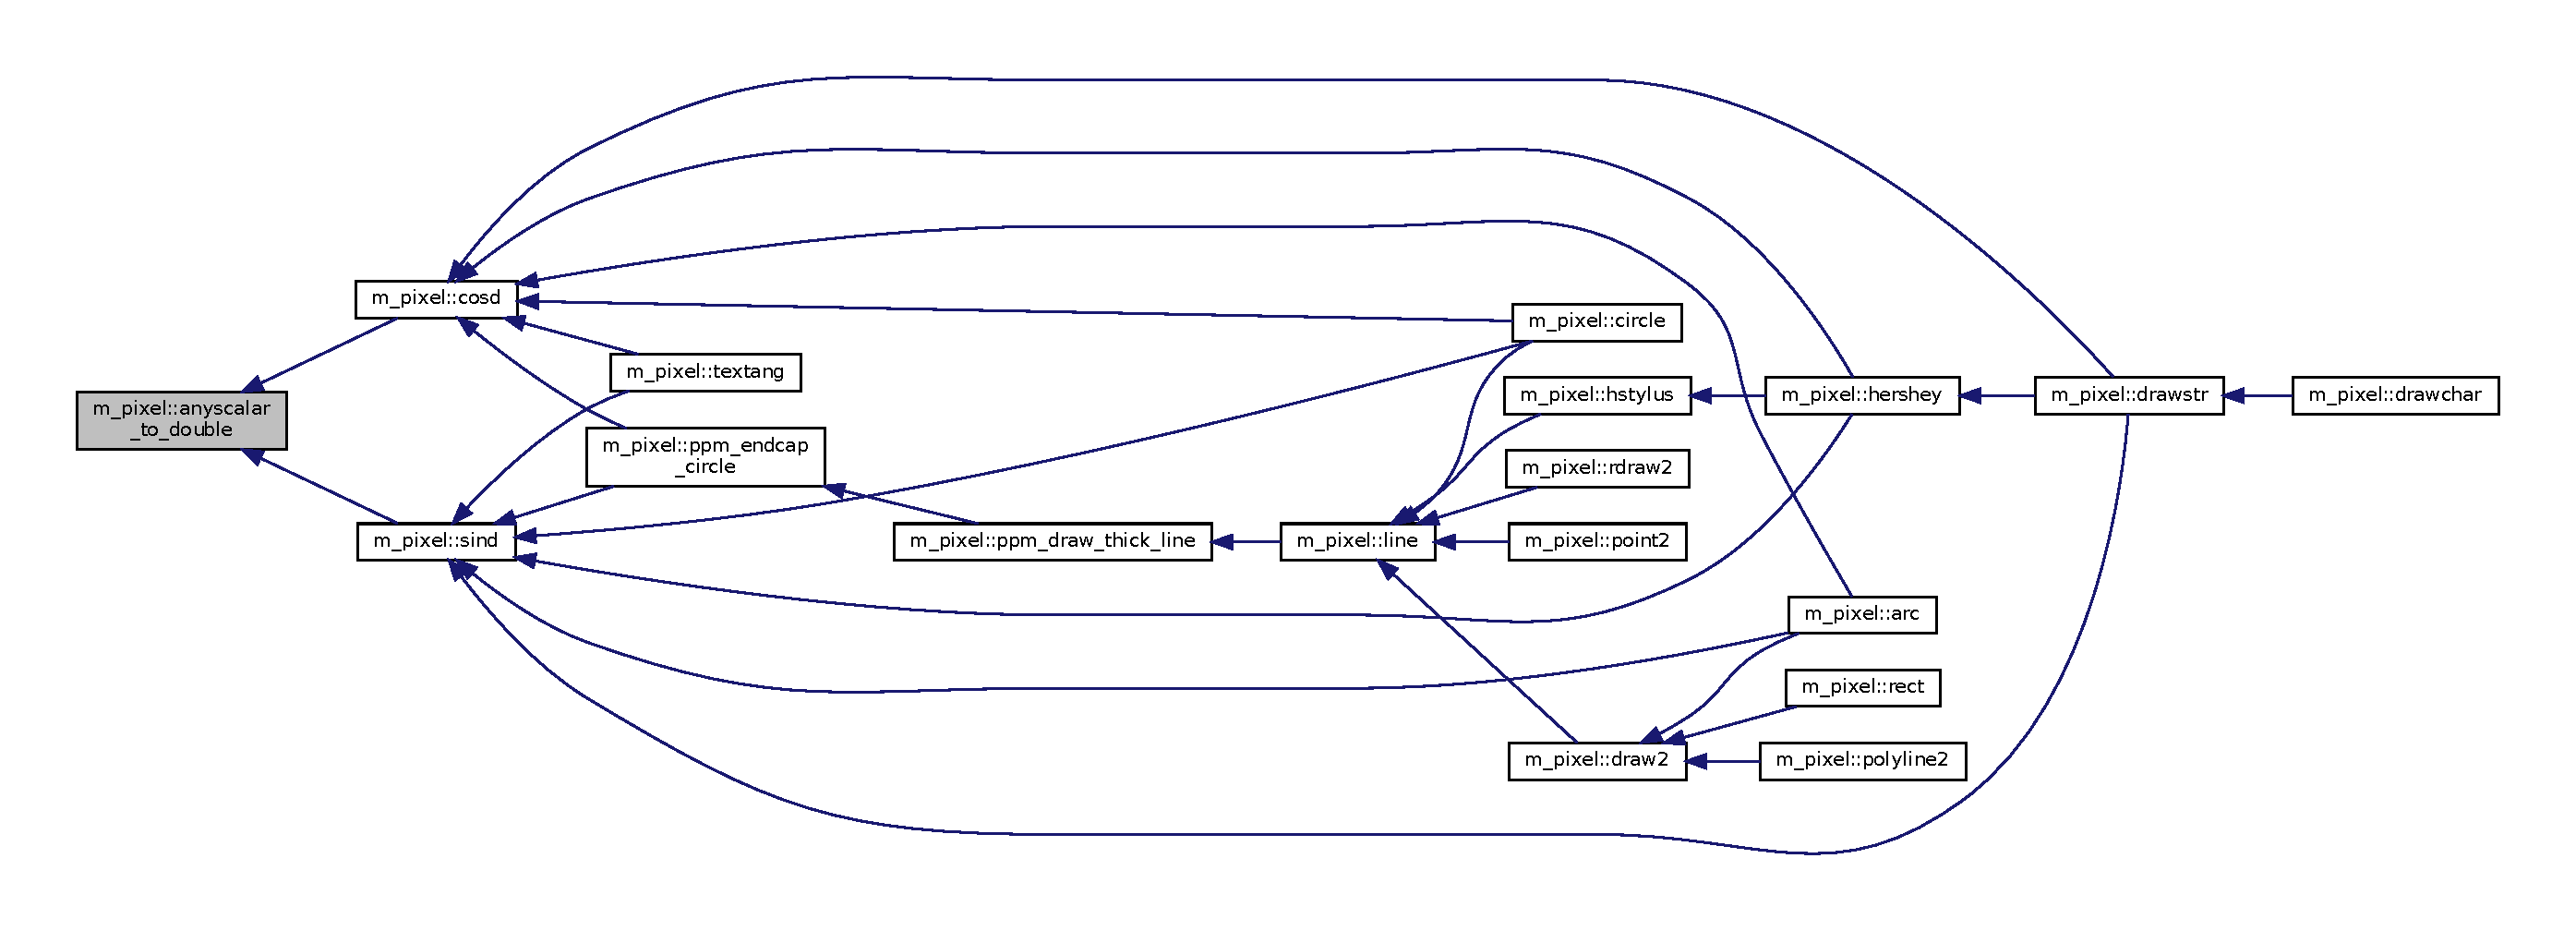
\includegraphics[width=350pt]{namespacem__pixel_a18d90bca3489d1280c4326e51b5cb7b3_icgraph}
\end{center}
\end{figure}
\mbox{\Hypertarget{namespacem__pixel_a79feab3c00d124d3f3396ad87ed4940e}\label{namespacem__pixel_a79feab3c00d124d3f3396ad87ed4940e}} 
\index{m\+\_\+pixel@{m\+\_\+pixel}!anyscalar\+\_\+to\+\_\+real@{anyscalar\+\_\+to\+\_\+real}}
\index{anyscalar\+\_\+to\+\_\+real@{anyscalar\+\_\+to\+\_\+real}!m\+\_\+pixel@{m\+\_\+pixel}}
\subsubsection{\texorpdfstring{anyscalar\+\_\+to\+\_\+real()}{anyscalar\_to\_real()}}
{\footnotesize\ttfamily pure elemental real function m\+\_\+pixel\+::anyscalar\+\_\+to\+\_\+real (\begin{DoxyParamCaption}\item[{class($\ast$), intent(in)}]{valuein }\end{DoxyParamCaption})\hspace{0.3cm}{\ttfamily [private]}}

Here is the caller graph for this function\+:
\nopagebreak
\begin{figure}[H]
\begin{center}
\leavevmode
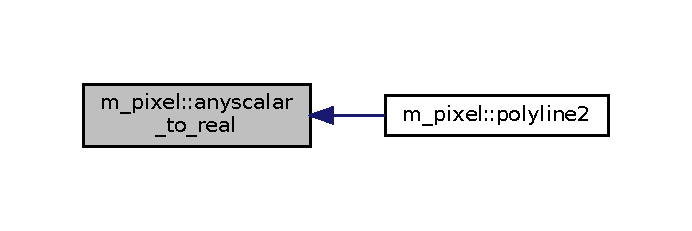
\includegraphics[width=332pt]{namespacem__pixel_a79feab3c00d124d3f3396ad87ed4940e_icgraph}
\end{center}
\end{figure}
\mbox{\Hypertarget{namespacem__pixel_ab881b9c2adff081a086cd83a1f1341fb}\label{namespacem__pixel_ab881b9c2adff081a086cd83a1f1341fb}} 
\index{m\+\_\+pixel@{m\+\_\+pixel}!arc@{arc}}
\index{arc@{arc}!m\+\_\+pixel@{m\+\_\+pixel}}
\subsubsection{\texorpdfstring{arc()}{arc()}}
{\footnotesize\ttfamily subroutine, public m\+\_\+pixel\+::arc (\begin{DoxyParamCaption}\item[{real, intent(in)}]{x,  }\item[{real, intent(in)}]{y,  }\item[{real, intent(in)}]{radius,  }\item[{real, intent(in)}]{startang,  }\item[{real, intent(in)}]{endang }\end{DoxyParamCaption})}



References cosd(), draw2(), move2(), p\+\_\+nsegs, and sind().

Here is the call graph for this function\+:
\nopagebreak
\begin{figure}[H]
\begin{center}
\leavevmode
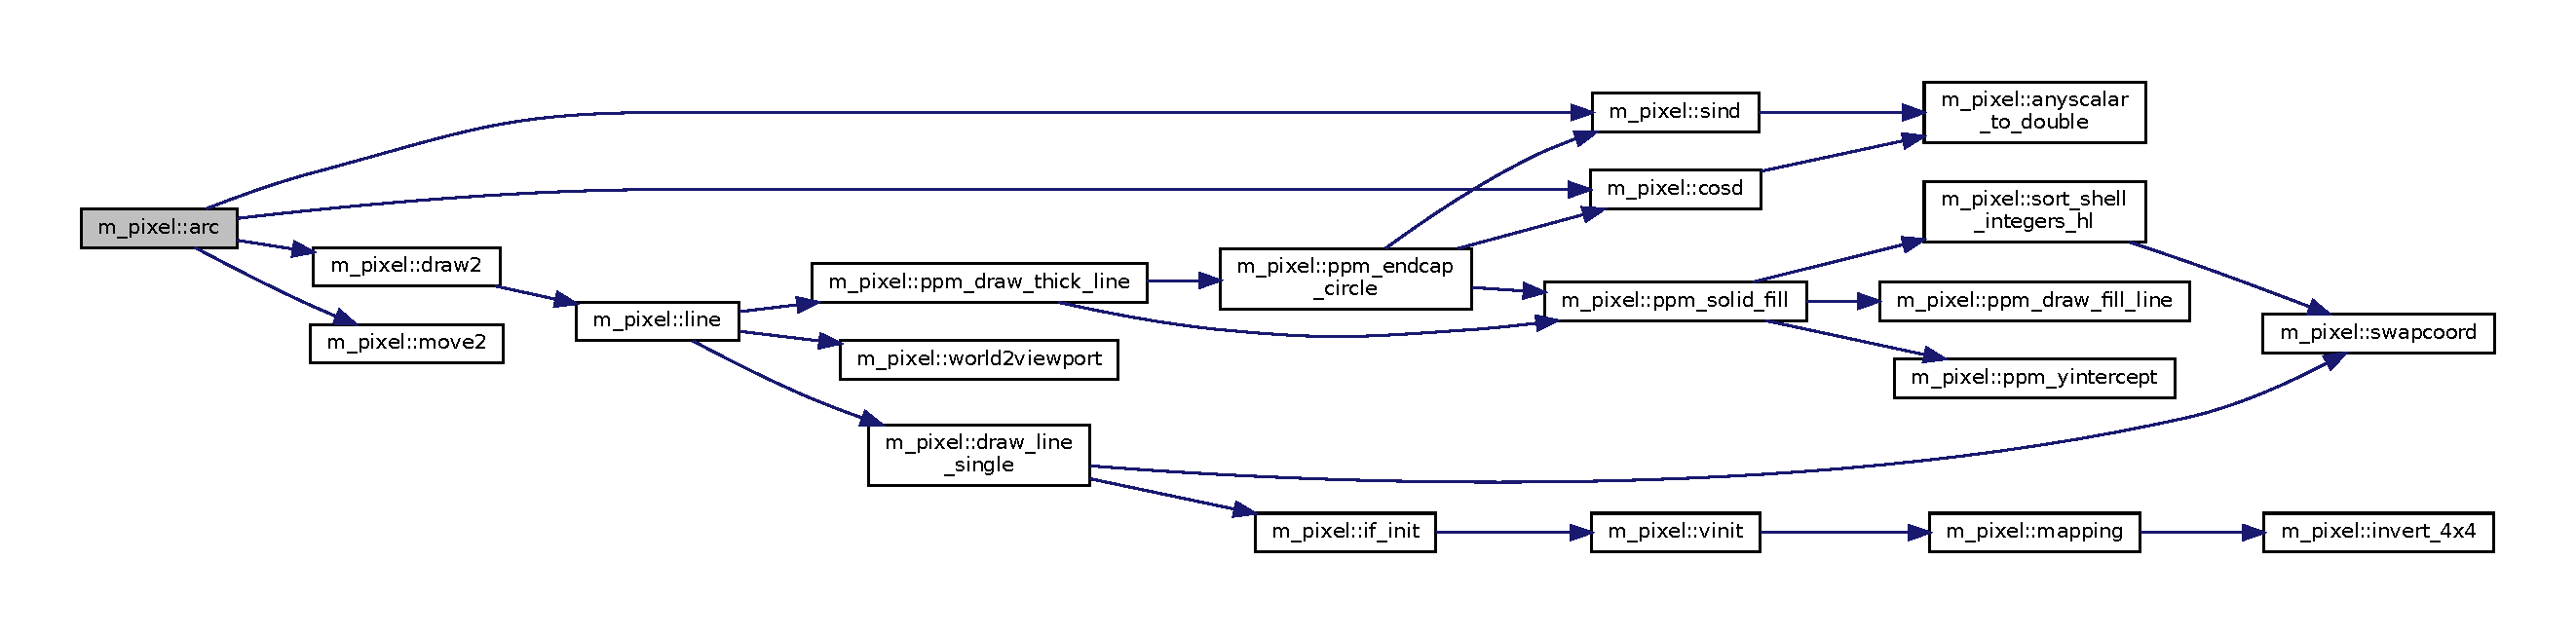
\includegraphics[width=350pt]{namespacem__pixel_ab881b9c2adff081a086cd83a1f1341fb_cgraph}
\end{center}
\end{figure}
\mbox{\Hypertarget{namespacem__pixel_a9ddc8e8604bbc3181c728f08a6b87904}\label{namespacem__pixel_a9ddc8e8604bbc3181c728f08a6b87904}} 
\index{m\+\_\+pixel@{m\+\_\+pixel}!centertext@{centertext}}
\index{centertext@{centertext}!m\+\_\+pixel@{m\+\_\+pixel}}
\subsubsection{\texorpdfstring{centertext()}{centertext()}}
{\footnotesize\ttfamily subroutine, public m\+\_\+pixel\+::centertext (\begin{DoxyParamCaption}\item[{logical, intent(in)}]{onoff }\end{DoxyParamCaption})}



References p\+\_\+x\+\_\+centertext, and p\+\_\+y\+\_\+centertext.

\mbox{\Hypertarget{namespacem__pixel_ab25c6cce708ff91a79bbabb23d591a8b}\label{namespacem__pixel_ab25c6cce708ff91a79bbabb23d591a8b}} 
\index{m\+\_\+pixel@{m\+\_\+pixel}!chrcod@{chrcod}}
\index{chrcod@{chrcod}!m\+\_\+pixel@{m\+\_\+pixel}}
\subsubsection{\texorpdfstring{chrcod()}{chrcod()}}
{\footnotesize\ttfamily subroutine m\+\_\+pixel\+::chrcod (\begin{DoxyParamCaption}\item[{character(len=$\ast$), intent(in)}]{text,  }\item[{integer, intent(in)}]{ntext }\end{DoxyParamCaption})\hspace{0.3cm}{\ttfamily [private]}}



References j, p\+\_\+ichr, p\+\_\+ioff, and p\+\_\+nchr.

Here is the caller graph for this function\+:
\nopagebreak
\begin{figure}[H]
\begin{center}
\leavevmode
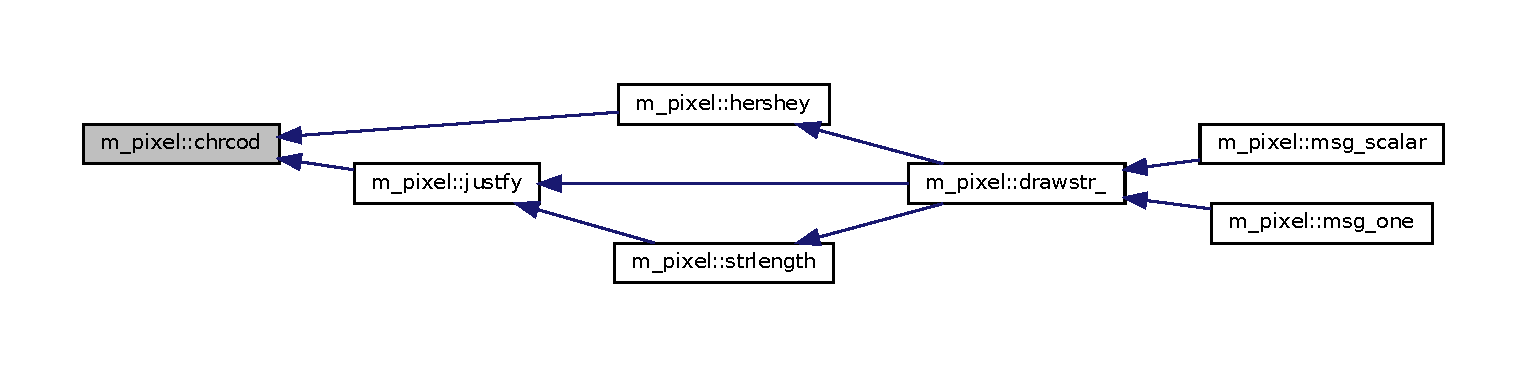
\includegraphics[width=350pt]{namespacem__pixel_ab25c6cce708ff91a79bbabb23d591a8b_icgraph}
\end{center}
\end{figure}
\mbox{\Hypertarget{namespacem__pixel_ab3b12cc498ed490014aa5fcc0bb278d2}\label{namespacem__pixel_ab3b12cc498ed490014aa5fcc0bb278d2}} 
\index{m\+\_\+pixel@{m\+\_\+pixel}!circle@{circle}}
\index{circle@{circle}!m\+\_\+pixel@{m\+\_\+pixel}}
\subsubsection{\texorpdfstring{circle()}{circle()}}
{\footnotesize\ttfamily subroutine, public m\+\_\+pixel\+::circle (\begin{DoxyParamCaption}\item[{real, intent(in)}]{x,  }\item[{real, intent(in)}]{y,  }\item[{real, intent(in)}]{radius }\end{DoxyParamCaption})}



References cosd(), line(), p\+\_\+nsegs, and sind().

Here is the call graph for this function\+:
\nopagebreak
\begin{figure}[H]
\begin{center}
\leavevmode
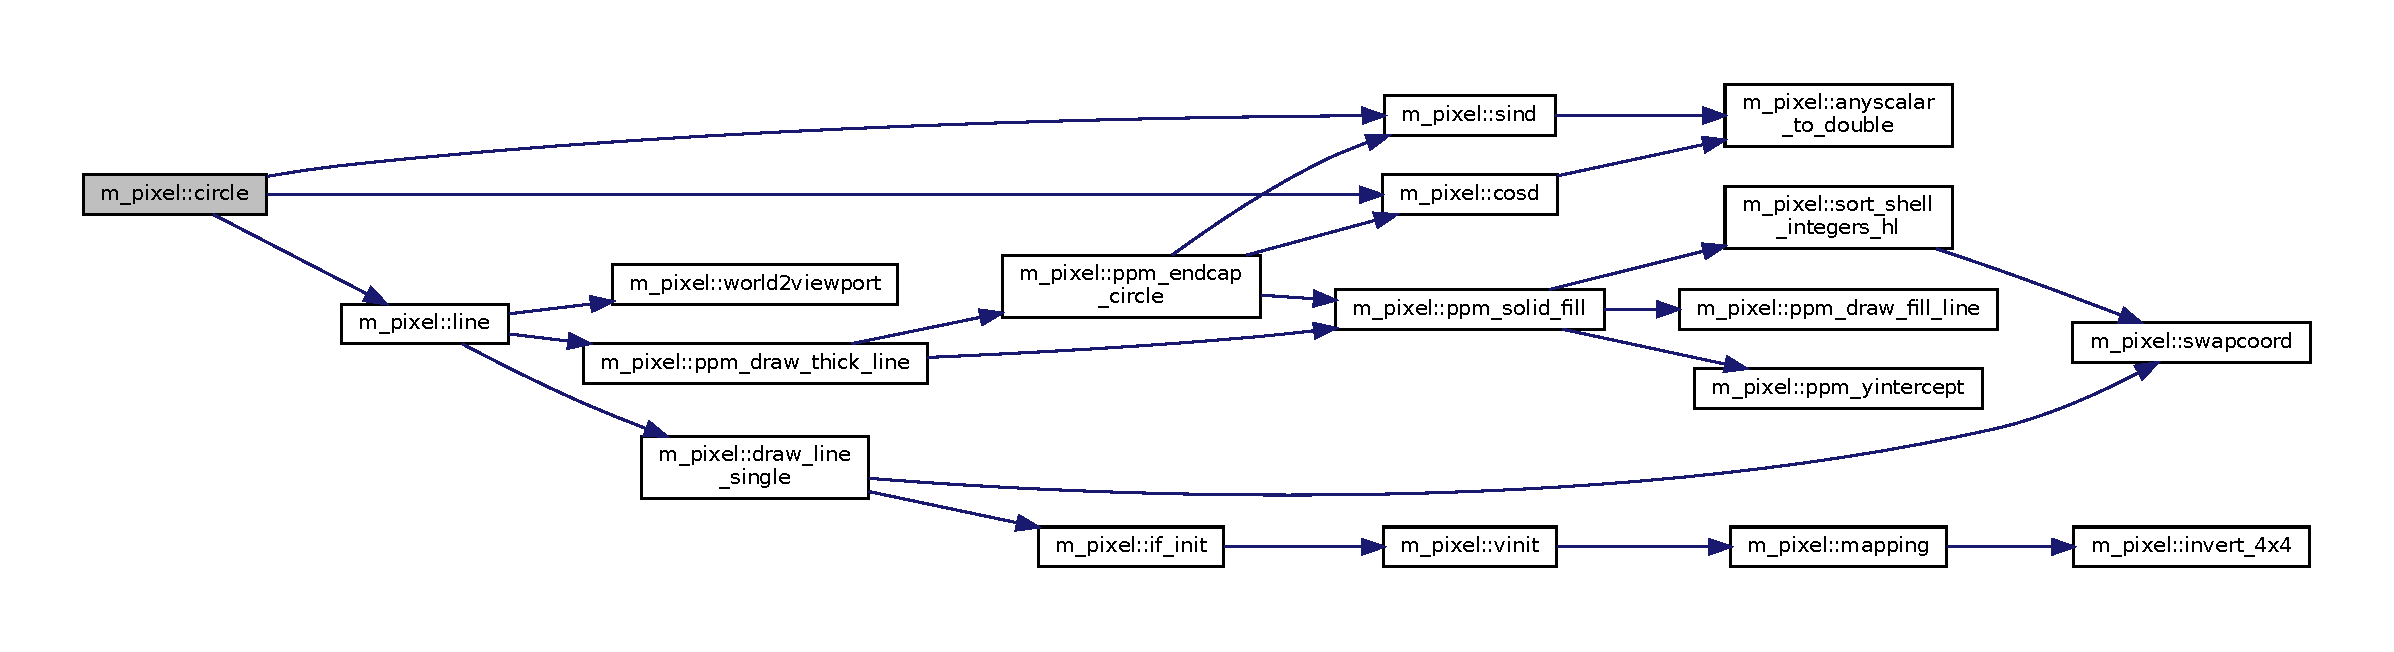
\includegraphics[width=350pt]{namespacem__pixel_ab3b12cc498ed490014aa5fcc0bb278d2_cgraph}
\end{center}
\end{figure}
\mbox{\Hypertarget{namespacem__pixel_a68ca1be8f7a92ece6efce8d69987af9c}\label{namespacem__pixel_a68ca1be8f7a92ece6efce8d69987af9c}} 
\index{m\+\_\+pixel@{m\+\_\+pixel}!circleprecision@{circleprecision}}
\index{circleprecision@{circleprecision}!m\+\_\+pixel@{m\+\_\+pixel}}
\subsubsection{\texorpdfstring{circleprecision()}{circleprecision()}}
{\footnotesize\ttfamily subroutine, public m\+\_\+pixel\+::circleprecision (\begin{DoxyParamCaption}\item[{integer, intent(in)}]{nsegs }\end{DoxyParamCaption})}



References p\+\_\+nsegs.

\mbox{\Hypertarget{namespacem__pixel_af3b81a21a0b2f6b5eddd09c031bd6173}\label{namespacem__pixel_af3b81a21a0b2f6b5eddd09c031bd6173}} 
\index{m\+\_\+pixel@{m\+\_\+pixel}!clear@{clear}}
\index{clear@{clear}!m\+\_\+pixel@{m\+\_\+pixel}}
\subsubsection{\texorpdfstring{clear()}{clear()}}
{\footnotesize\ttfamily subroutine, public m\+\_\+pixel\+::clear (\begin{DoxyParamCaption}\item[{integer, intent(in), optional}]{indx }\end{DoxyParamCaption})}



References if\+\_\+init(), p\+\_\+color\+\_\+index, and p\+\_\+pixel.

Here is the call graph for this function\+:
\nopagebreak
\begin{figure}[H]
\begin{center}
\leavevmode
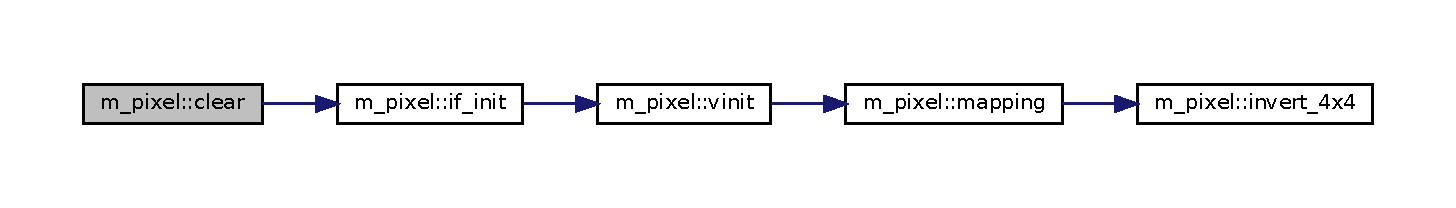
\includegraphics[width=350pt]{namespacem__pixel_af3b81a21a0b2f6b5eddd09c031bd6173_cgraph}
\end{center}
\end{figure}
Here is the caller graph for this function\+:
\nopagebreak
\begin{figure}[H]
\begin{center}
\leavevmode
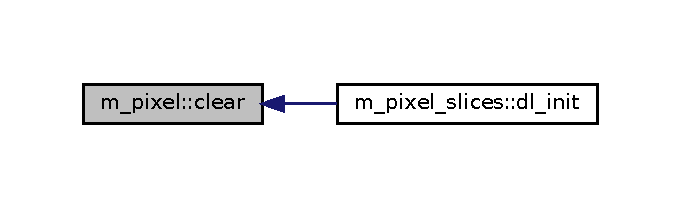
\includegraphics[width=327pt]{namespacem__pixel_af3b81a21a0b2f6b5eddd09c031bd6173_icgraph}
\end{center}
\end{figure}
\mbox{\Hypertarget{namespacem__pixel_ab3dc83b63d2ab1bf3f63932abca4245d}\label{namespacem__pixel_ab3dc83b63d2ab1bf3f63932abca4245d}} 
\index{m\+\_\+pixel@{m\+\_\+pixel}!closepoly@{closepoly}}
\index{closepoly@{closepoly}!m\+\_\+pixel@{m\+\_\+pixel}}
\subsubsection{\texorpdfstring{closepoly()}{closepoly()}}
{\footnotesize\ttfamily subroutine, public m\+\_\+pixel\+::closepoly (\begin{DoxyParamCaption}{ }\end{DoxyParamCaption})}



References p\+\_\+inpolygon, p\+\_\+polypoints, p\+\_\+polyvertex, and poly2().

Here is the call graph for this function\+:
\nopagebreak
\begin{figure}[H]
\begin{center}
\leavevmode
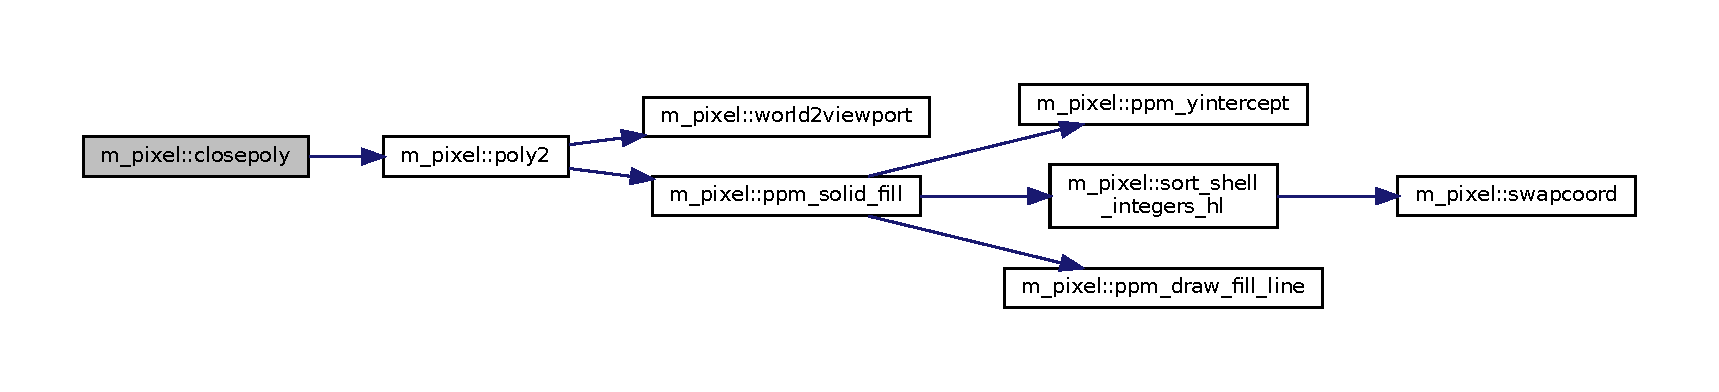
\includegraphics[width=350pt]{namespacem__pixel_ab3dc83b63d2ab1bf3f63932abca4245d_cgraph}
\end{center}
\end{figure}
\mbox{\Hypertarget{namespacem__pixel_a8555eecec7e18106e8167e137cfe8424}\label{namespacem__pixel_a8555eecec7e18106e8167e137cfe8424}} 
\index{m\+\_\+pixel@{m\+\_\+pixel}!closest\+\_\+color\+\_\+name@{closest\+\_\+color\+\_\+name}}
\index{closest\+\_\+color\+\_\+name@{closest\+\_\+color\+\_\+name}!m\+\_\+pixel@{m\+\_\+pixel}}
\subsubsection{\texorpdfstring{closest\+\_\+color\+\_\+name()}{closest\_color\_name()}}
{\footnotesize\ttfamily subroutine, public m\+\_\+pixel\+::closest\+\_\+color\+\_\+name (\begin{DoxyParamCaption}\item[{real, intent(in)}]{r,  }\item[{real, intent(in)}]{g,  }\item[{real, intent(in)}]{b,  }\item[{character(len=$\ast$), intent(out)}]{closestname }\end{DoxyParamCaption})}



References color\+\_\+name2rgb(), and i2s().

Here is the call graph for this function\+:
\nopagebreak
\begin{figure}[H]
\begin{center}
\leavevmode
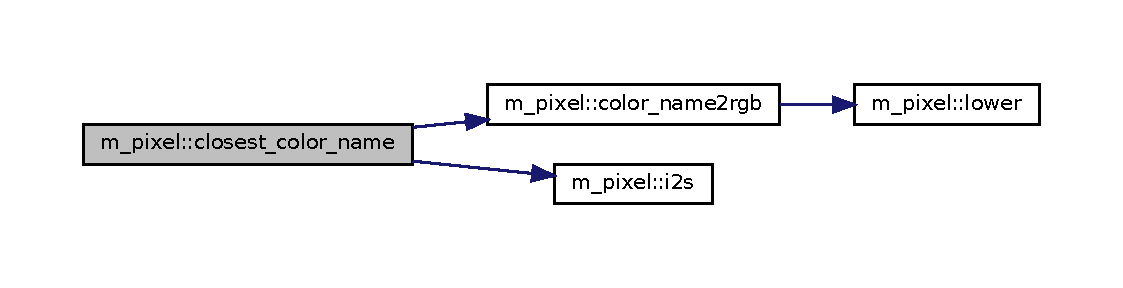
\includegraphics[width=350pt]{namespacem__pixel_a8555eecec7e18106e8167e137cfe8424_cgraph}
\end{center}
\end{figure}
\mbox{\Hypertarget{namespacem__pixel_a98c49513d301803bb2c5cd28b8ccdba3}\label{namespacem__pixel_a98c49513d301803bb2c5cd28b8ccdba3}} 
\index{m\+\_\+pixel@{m\+\_\+pixel}!cmyrgb@{cmyrgb}}
\index{cmyrgb@{cmyrgb}!m\+\_\+pixel@{m\+\_\+pixel}}
\subsubsection{\texorpdfstring{cmyrgb()}{cmyrgb()}}
{\footnotesize\ttfamily subroutine, private m\+\_\+pixel\+::cmyrgb (\begin{DoxyParamCaption}\item[{real, intent(in)}]{c,  }\item[{real, intent(in)}]{m,  }\item[{real, intent(in)}]{y,  }\item[{real, intent(out)}]{r,  }\item[{real, intent(out)}]{g,  }\item[{real, intent(out)}]{b,  }\item[{integer}]{status }\end{DoxyParamCaption})\hspace{0.3cm}{\ttfamily [private]}}

Here is the caller graph for this function\+:
\nopagebreak
\begin{figure}[H]
\begin{center}
\leavevmode
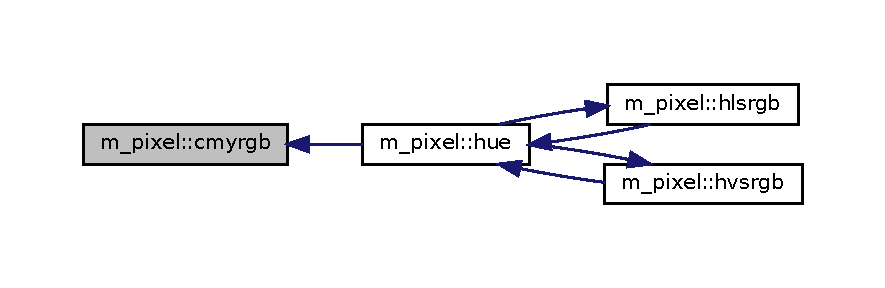
\includegraphics[width=350pt]{namespacem__pixel_a98c49513d301803bb2c5cd28b8ccdba3_icgraph}
\end{center}
\end{figure}
\mbox{\Hypertarget{namespacem__pixel_a334bde41bc7b2db19b950b1271ba7463}\label{namespacem__pixel_a334bde41bc7b2db19b950b1271ba7463}} 
\index{m\+\_\+pixel@{m\+\_\+pixel}!color@{color}}
\index{color@{color}!m\+\_\+pixel@{m\+\_\+pixel}}
\subsubsection{\texorpdfstring{color()}{color()}}
{\footnotesize\ttfamily subroutine, public m\+\_\+pixel\+::color (\begin{DoxyParamCaption}\item[{integer, intent(in)}]{icolor }\end{DoxyParamCaption})}



References p\+\_\+color\+\_\+index.

Here is the caller graph for this function\+:
\nopagebreak
\begin{figure}[H]
\begin{center}
\leavevmode
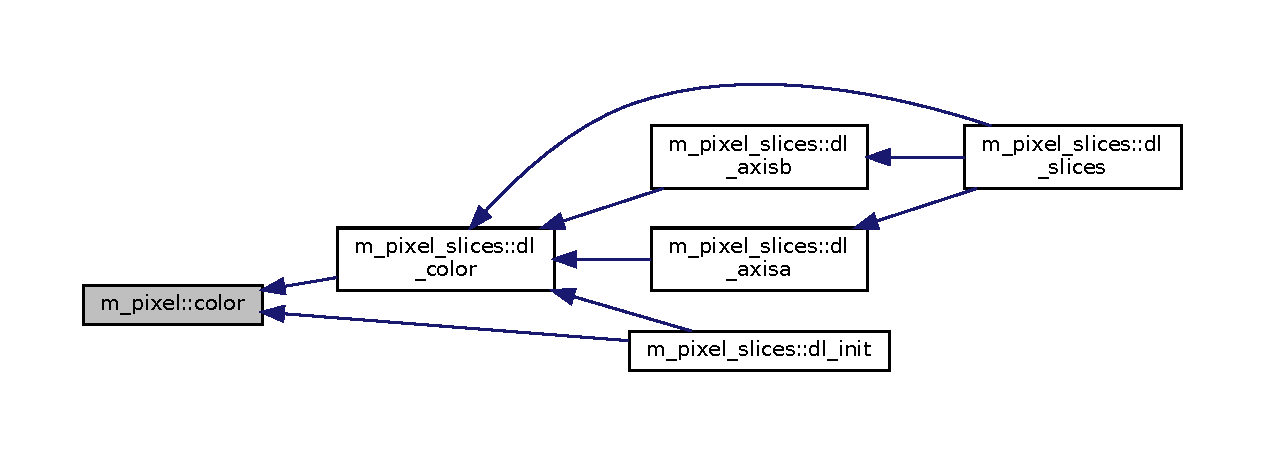
\includegraphics[width=350pt]{namespacem__pixel_a334bde41bc7b2db19b950b1271ba7463_icgraph}
\end{center}
\end{figure}
\mbox{\Hypertarget{namespacem__pixel_aee26ac45961d4093d2e472fcb6e1887d}\label{namespacem__pixel_aee26ac45961d4093d2e472fcb6e1887d}} 
\index{m\+\_\+pixel@{m\+\_\+pixel}!color\+\_\+name2rgb@{color\+\_\+name2rgb}}
\index{color\+\_\+name2rgb@{color\+\_\+name2rgb}!m\+\_\+pixel@{m\+\_\+pixel}}
\subsubsection{\texorpdfstring{color\+\_\+name2rgb()}{color\_name2rgb()}}
{\footnotesize\ttfamily subroutine, public m\+\_\+pixel\+::color\+\_\+name2rgb (\begin{DoxyParamCaption}\item[{character(len=$\ast$), intent(in)}]{name,  }\item[{real, intent(out)}]{r,  }\item[{real, intent(out)}]{g,  }\item[{real, intent(out)}]{b,  }\item[{character(len=$\ast$), intent(out), optional}]{echoname }\end{DoxyParamCaption})}



References lower().

Here is the call graph for this function\+:
\nopagebreak
\begin{figure}[H]
\begin{center}
\leavevmode
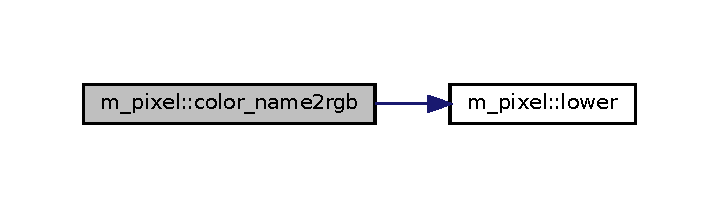
\includegraphics[width=345pt]{namespacem__pixel_aee26ac45961d4093d2e472fcb6e1887d_cgraph}
\end{center}
\end{figure}
Here is the caller graph for this function\+:
\nopagebreak
\begin{figure}[H]
\begin{center}
\leavevmode
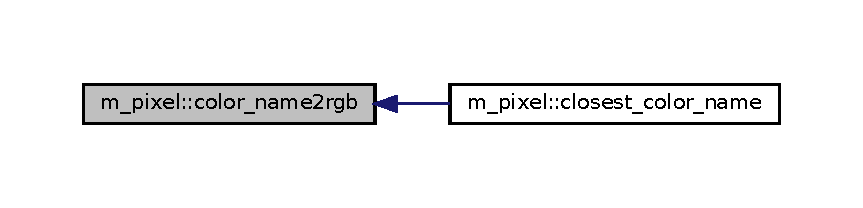
\includegraphics[width=350pt]{namespacem__pixel_aee26ac45961d4093d2e472fcb6e1887d_icgraph}
\end{center}
\end{figure}
\mbox{\Hypertarget{namespacem__pixel_a312c40bfbd03b2bbe6f85bc5efca6ce3}\label{namespacem__pixel_a312c40bfbd03b2bbe6f85bc5efca6ce3}} 
\index{m\+\_\+pixel@{m\+\_\+pixel}!cosd@{cosd}}
\index{cosd@{cosd}!m\+\_\+pixel@{m\+\_\+pixel}}
\subsubsection{\texorpdfstring{cosd()}{cosd()}}
{\footnotesize\ttfamily elemental real function, public m\+\_\+pixel\+::cosd (\begin{DoxyParamCaption}\item[{class($\ast$), intent(in)}]{angle\+\_\+in\+\_\+degrees }\end{DoxyParamCaption})}



References anyscalar\+\_\+to\+\_\+double(), and degrees\+\_\+to\+\_\+radians.

Here is the call graph for this function\+:
\nopagebreak
\begin{figure}[H]
\begin{center}
\leavevmode
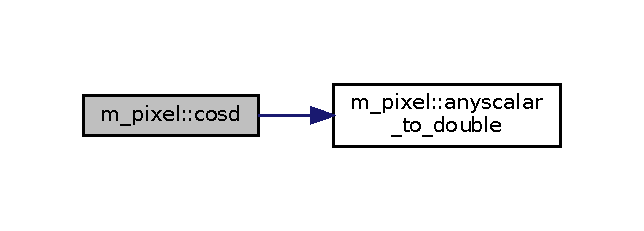
\includegraphics[width=309pt]{namespacem__pixel_a312c40bfbd03b2bbe6f85bc5efca6ce3_cgraph}
\end{center}
\end{figure}
Here is the caller graph for this function\+:
\nopagebreak
\begin{figure}[H]
\begin{center}
\leavevmode
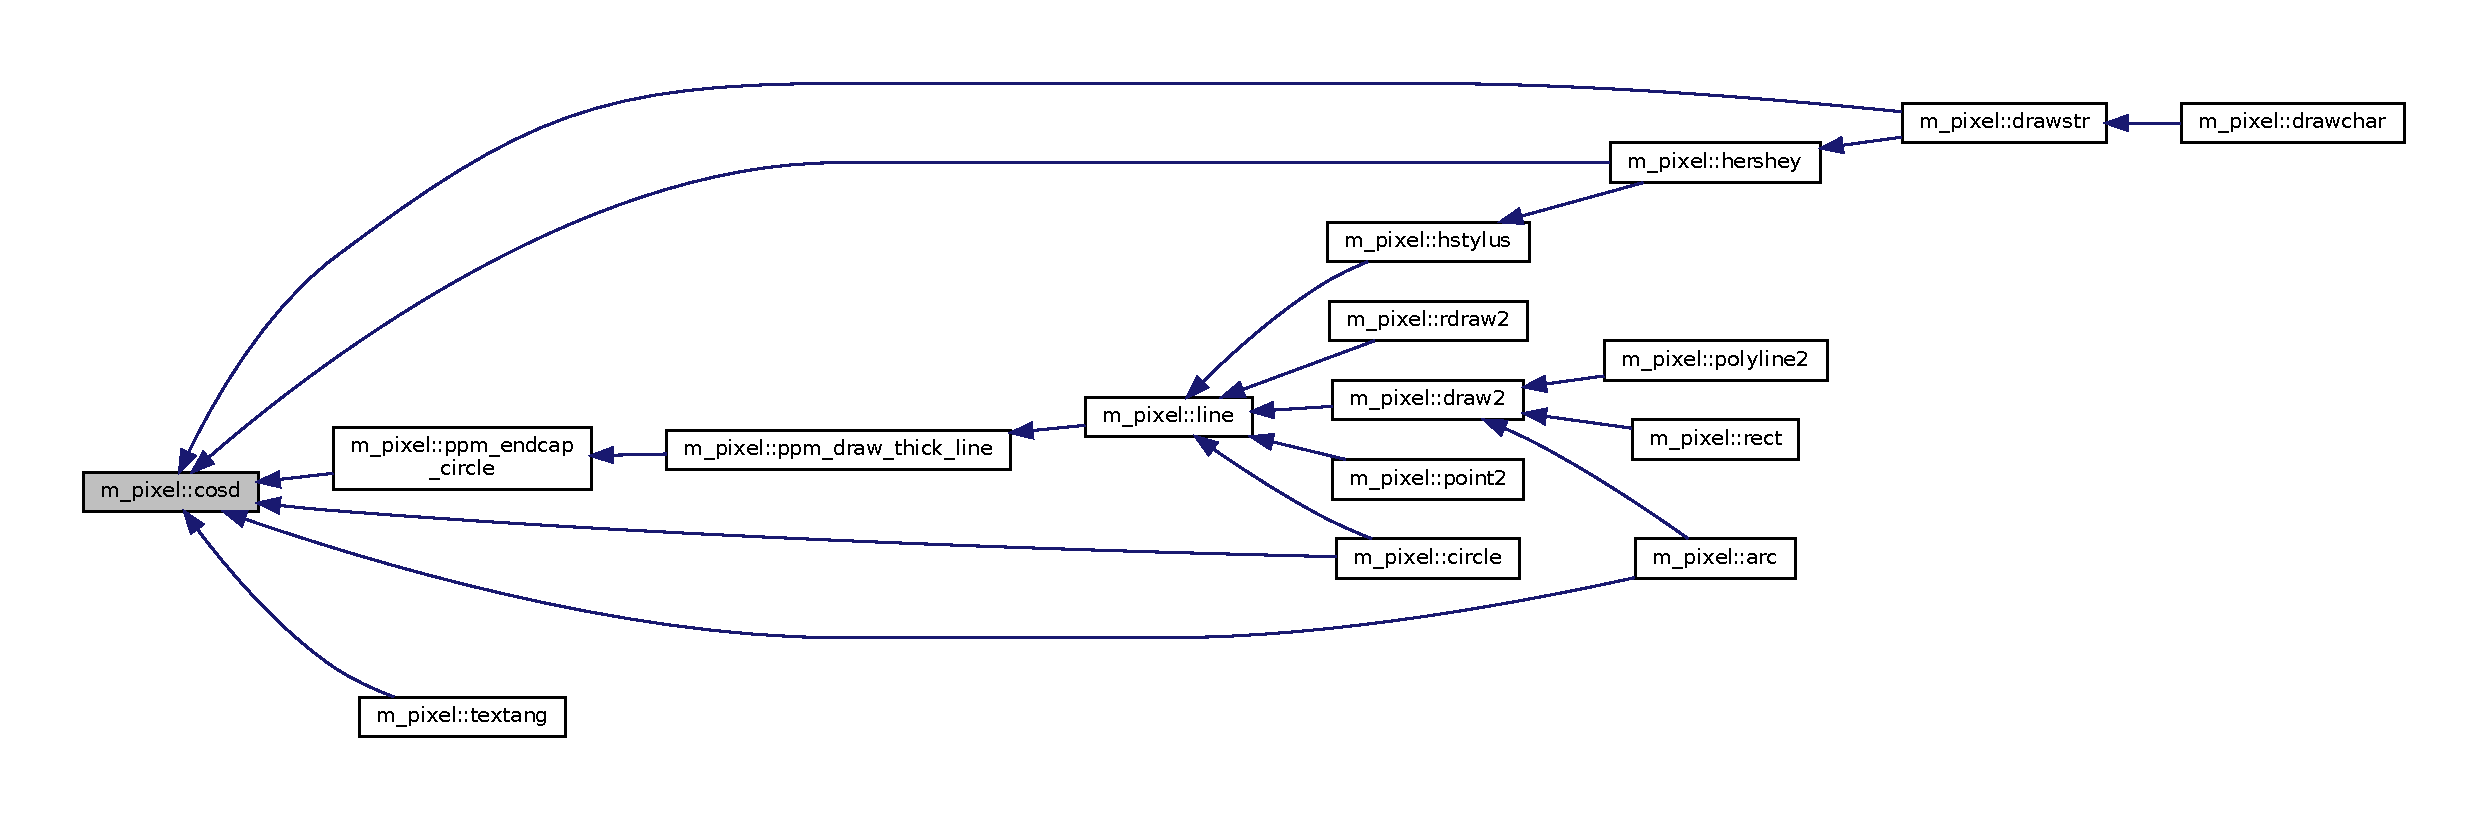
\includegraphics[width=350pt]{namespacem__pixel_a312c40bfbd03b2bbe6f85bc5efca6ce3_icgraph}
\end{center}
\end{figure}
\mbox{\Hypertarget{namespacem__pixel_a2ea42e55432274dec04fdc822e484cdb}\label{namespacem__pixel_a2ea42e55432274dec04fdc822e484cdb}} 
\index{m\+\_\+pixel@{m\+\_\+pixel}!d2r\+\_\+d@{d2r\+\_\+d}}
\index{d2r\+\_\+d@{d2r\+\_\+d}!m\+\_\+pixel@{m\+\_\+pixel}}
\subsubsection{\texorpdfstring{d2r\+\_\+d()}{d2r\_d()}}
{\footnotesize\ttfamily elemental doubleprecision function m\+\_\+pixel\+::d2r\+\_\+d (\begin{DoxyParamCaption}\item[{doubleprecision, intent(in)}]{degrees }\end{DoxyParamCaption})\hspace{0.3cm}{\ttfamily [private]}}

\mbox{\Hypertarget{namespacem__pixel_a0ac7088105ca5334d0ca3f1e4ea16d65}\label{namespacem__pixel_a0ac7088105ca5334d0ca3f1e4ea16d65}} 
\index{m\+\_\+pixel@{m\+\_\+pixel}!d2r\+\_\+i@{d2r\+\_\+i}}
\index{d2r\+\_\+i@{d2r\+\_\+i}!m\+\_\+pixel@{m\+\_\+pixel}}
\subsubsection{\texorpdfstring{d2r\+\_\+i()}{d2r\_i()}}
{\footnotesize\ttfamily elemental doubleprecision function m\+\_\+pixel\+::d2r\+\_\+i (\begin{DoxyParamCaption}\item[{integer, intent(in)}]{idegrees }\end{DoxyParamCaption})\hspace{0.3cm}{\ttfamily [private]}}

\mbox{\Hypertarget{namespacem__pixel_af1963e62c5cc06bfb042831d1c869dc1}\label{namespacem__pixel_af1963e62c5cc06bfb042831d1c869dc1}} 
\index{m\+\_\+pixel@{m\+\_\+pixel}!d2r\+\_\+r@{d2r\+\_\+r}}
\index{d2r\+\_\+r@{d2r\+\_\+r}!m\+\_\+pixel@{m\+\_\+pixel}}
\subsubsection{\texorpdfstring{d2r\+\_\+r()}{d2r\_r()}}
{\footnotesize\ttfamily elemental real function m\+\_\+pixel\+::d2r\+\_\+r (\begin{DoxyParamCaption}\item[{real, intent(in)}]{degrees }\end{DoxyParamCaption})\hspace{0.3cm}{\ttfamily [private]}}

\mbox{\Hypertarget{namespacem__pixel_a12012e819bb14b27d2b49732aa2e4e55}\label{namespacem__pixel_a12012e819bb14b27d2b49732aa2e4e55}} 
\index{m\+\_\+pixel@{m\+\_\+pixel}!draw2@{draw2}}
\index{draw2@{draw2}!m\+\_\+pixel@{m\+\_\+pixel}}
\subsubsection{\texorpdfstring{draw2()}{draw2()}}
{\footnotesize\ttfamily subroutine, public m\+\_\+pixel\+::draw2 (\begin{DoxyParamCaption}\item[{real, intent(in)}]{x,  }\item[{real, intent(in)}]{y }\end{DoxyParamCaption})}



References line(), p\+\_\+x, and p\+\_\+y.

Here is the call graph for this function\+:
\nopagebreak
\begin{figure}[H]
\begin{center}
\leavevmode
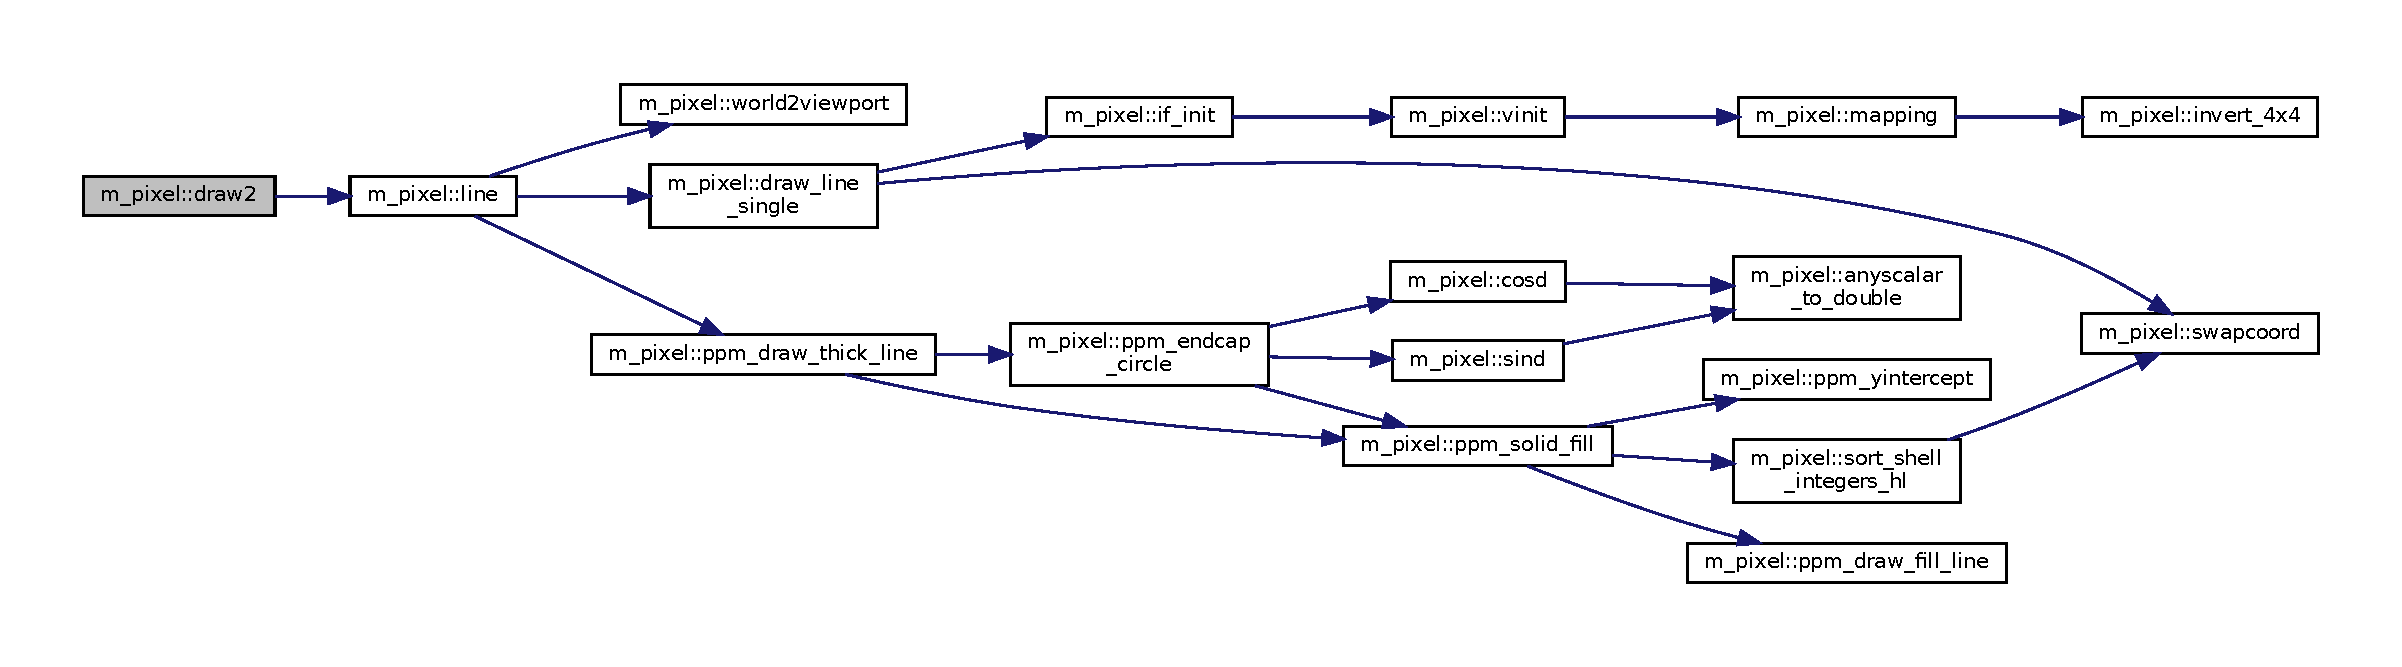
\includegraphics[width=350pt]{namespacem__pixel_a12012e819bb14b27d2b49732aa2e4e55_cgraph}
\end{center}
\end{figure}
Here is the caller graph for this function\+:
\nopagebreak
\begin{figure}[H]
\begin{center}
\leavevmode
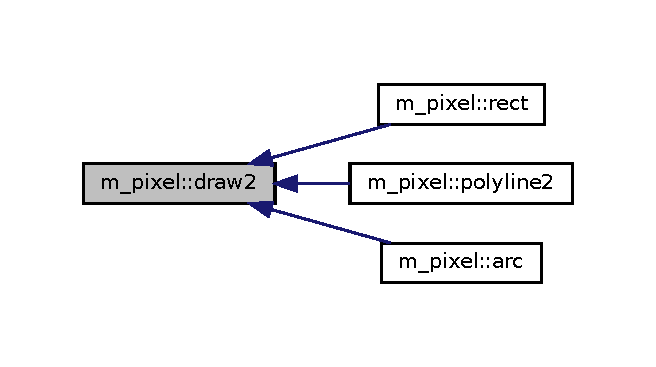
\includegraphics[width=350pt]{namespacem__pixel_a12012e819bb14b27d2b49732aa2e4e55_icgraph}
\end{center}
\end{figure}
\mbox{\Hypertarget{namespacem__pixel_a42791c7e58158616dae7c36ec5806717}\label{namespacem__pixel_a42791c7e58158616dae7c36ec5806717}} 
\index{m\+\_\+pixel@{m\+\_\+pixel}!draw\+\_\+line\+\_\+single@{draw\+\_\+line\+\_\+single}}
\index{draw\+\_\+line\+\_\+single@{draw\+\_\+line\+\_\+single}!m\+\_\+pixel@{m\+\_\+pixel}}
\subsubsection{\texorpdfstring{draw\+\_\+line\+\_\+single()}{draw\_line\_single()}}
{\footnotesize\ttfamily subroutine m\+\_\+pixel\+::draw\+\_\+line\+\_\+single (\begin{DoxyParamCaption}\item[{integer, intent(in)}]{x1,  }\item[{integer, intent(in)}]{y1,  }\item[{integer, intent(in)}]{x2,  }\item[{integer, intent(in)}]{y2 }\end{DoxyParamCaption})\hspace{0.3cm}{\ttfamily [private]}}



References if\+\_\+init(), p\+\_\+color\+\_\+index, p\+\_\+debug, p\+\_\+pixel, and swapcoord().

Here is the call graph for this function\+:
\nopagebreak
\begin{figure}[H]
\begin{center}
\leavevmode
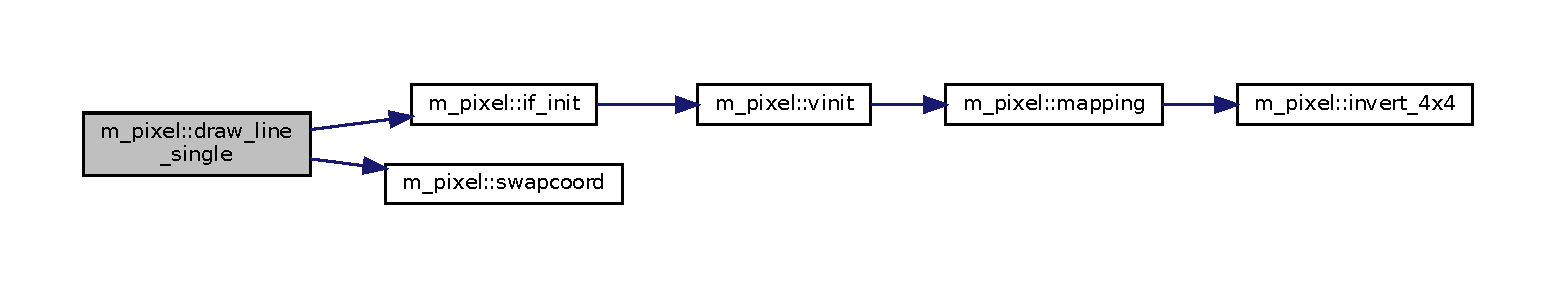
\includegraphics[width=350pt]{namespacem__pixel_a42791c7e58158616dae7c36ec5806717_cgraph}
\end{center}
\end{figure}
Here is the caller graph for this function\+:
\nopagebreak
\begin{figure}[H]
\begin{center}
\leavevmode
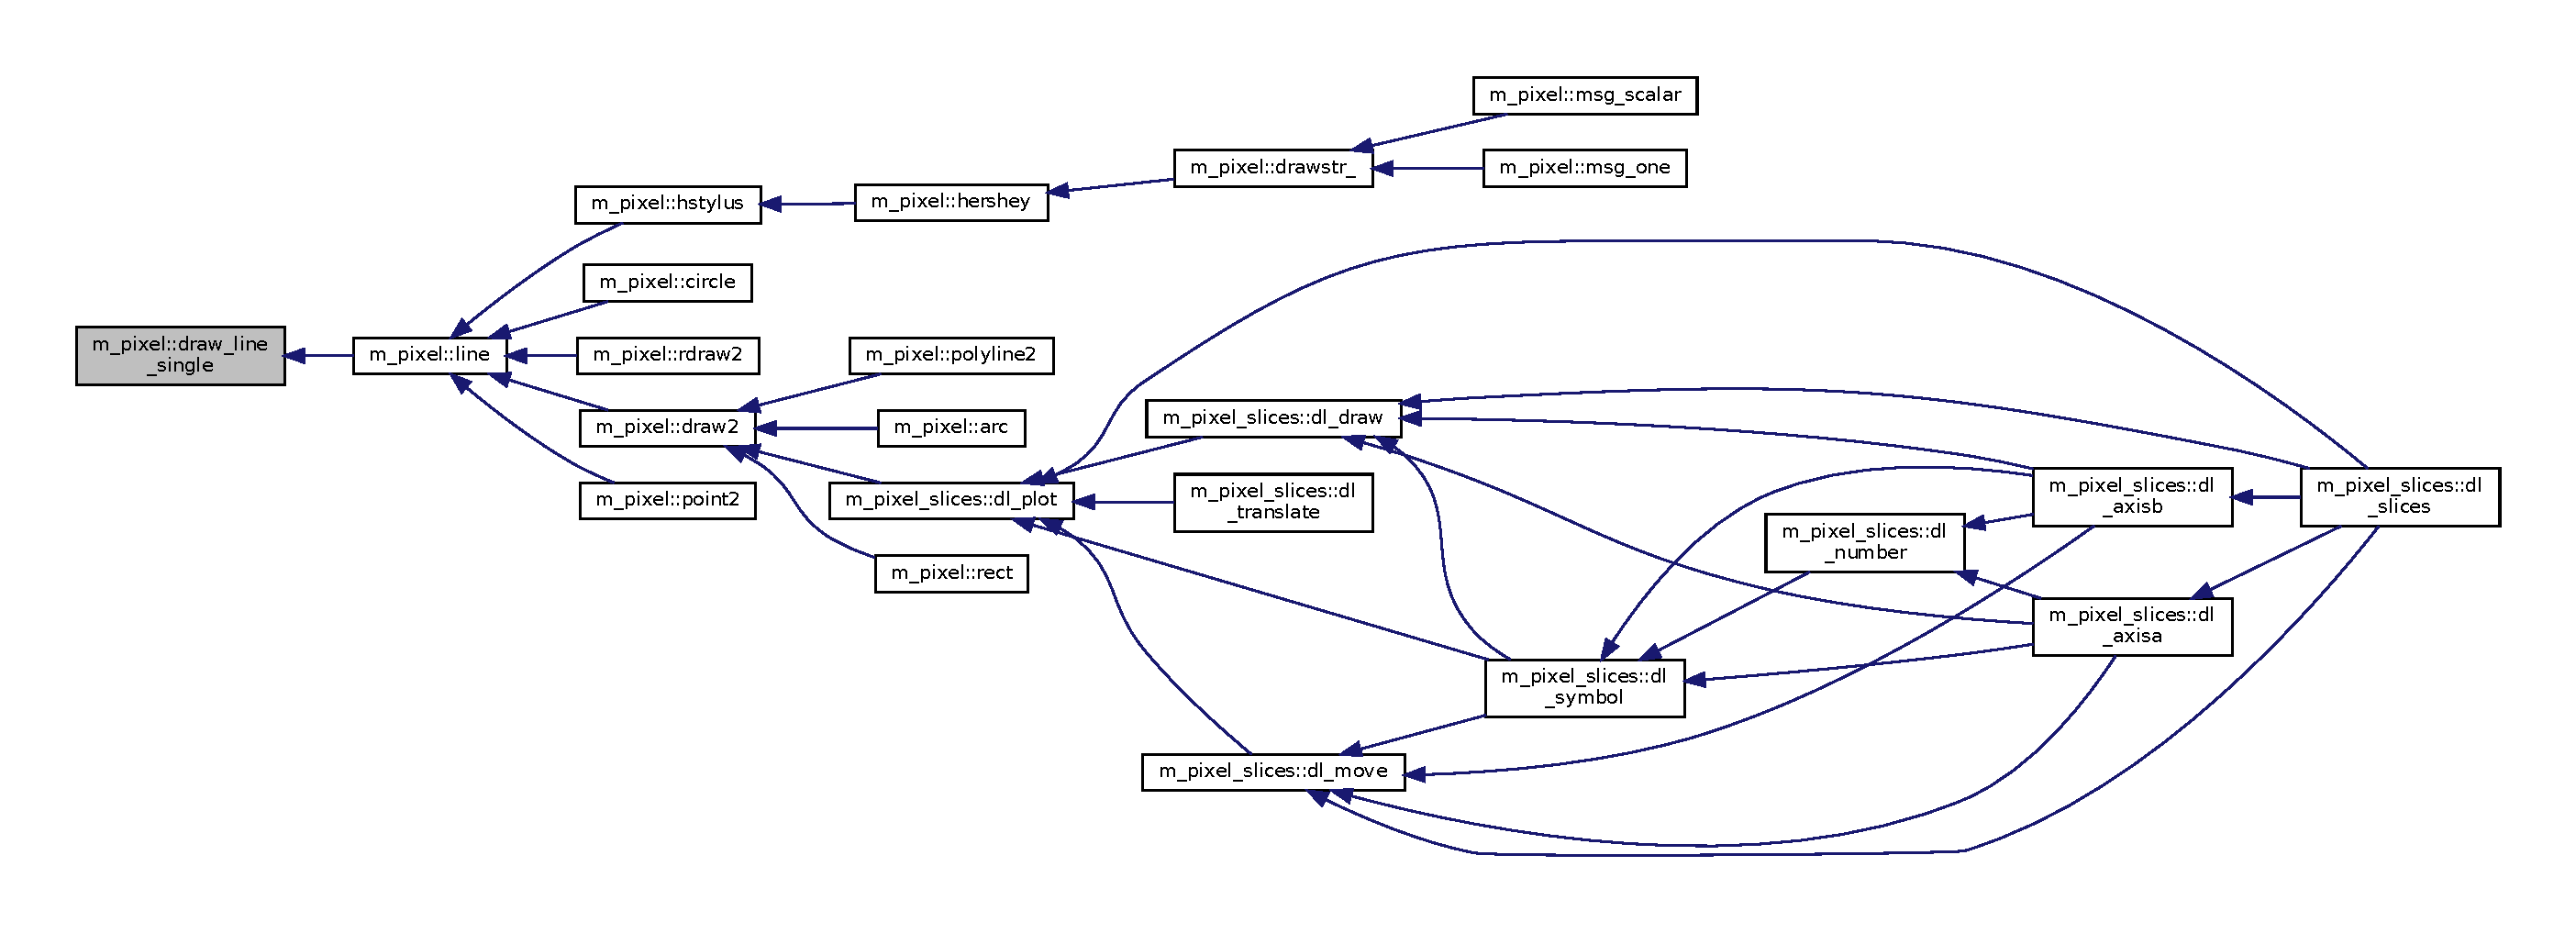
\includegraphics[width=350pt]{namespacem__pixel_a42791c7e58158616dae7c36ec5806717_icgraph}
\end{center}
\end{figure}
\mbox{\Hypertarget{namespacem__pixel_a58406ffd6c2a9fdf2ea7772198b54255}\label{namespacem__pixel_a58406ffd6c2a9fdf2ea7772198b54255}} 
\index{m\+\_\+pixel@{m\+\_\+pixel}!drawchar@{drawchar}}
\index{drawchar@{drawchar}!m\+\_\+pixel@{m\+\_\+pixel}}
\subsubsection{\texorpdfstring{drawchar()}{drawchar()}}
{\footnotesize\ttfamily subroutine, public m\+\_\+pixel\+::drawchar (\begin{DoxyParamCaption}\item[{character(len=1), intent(in)}]{ch }\end{DoxyParamCaption})}

\mbox{\Hypertarget{namespacem__pixel_a3f8850328e359af5802954b2f70652f5}\label{namespacem__pixel_a3f8850328e359af5802954b2f70652f5}} 
\index{m\+\_\+pixel@{m\+\_\+pixel}!drawstr\+\_\+@{drawstr\+\_\+}}
\index{drawstr\+\_\+@{drawstr\+\_\+}!m\+\_\+pixel@{m\+\_\+pixel}}
\subsubsection{\texorpdfstring{drawstr\+\_\+()}{drawstr\_()}}
{\footnotesize\ttfamily subroutine m\+\_\+pixel\+::drawstr\+\_\+ (\begin{DoxyParamCaption}\item[{character(len=$\ast$), intent(in)}]{string }\end{DoxyParamCaption})\hspace{0.3cm}{\ttfamily [private]}}



References cosd(), hershey(), justfy(), move2(), p\+\_\+text\+\_\+angle, p\+\_\+text\+\_\+cosine, p\+\_\+text\+\_\+height, p\+\_\+text\+\_\+sine, p\+\_\+x, p\+\_\+x\+\_\+centertext, p\+\_\+y, p\+\_\+y\+\_\+centertext, sind(), and strlength().

Here is the call graph for this function\+:
\nopagebreak
\begin{figure}[H]
\begin{center}
\leavevmode
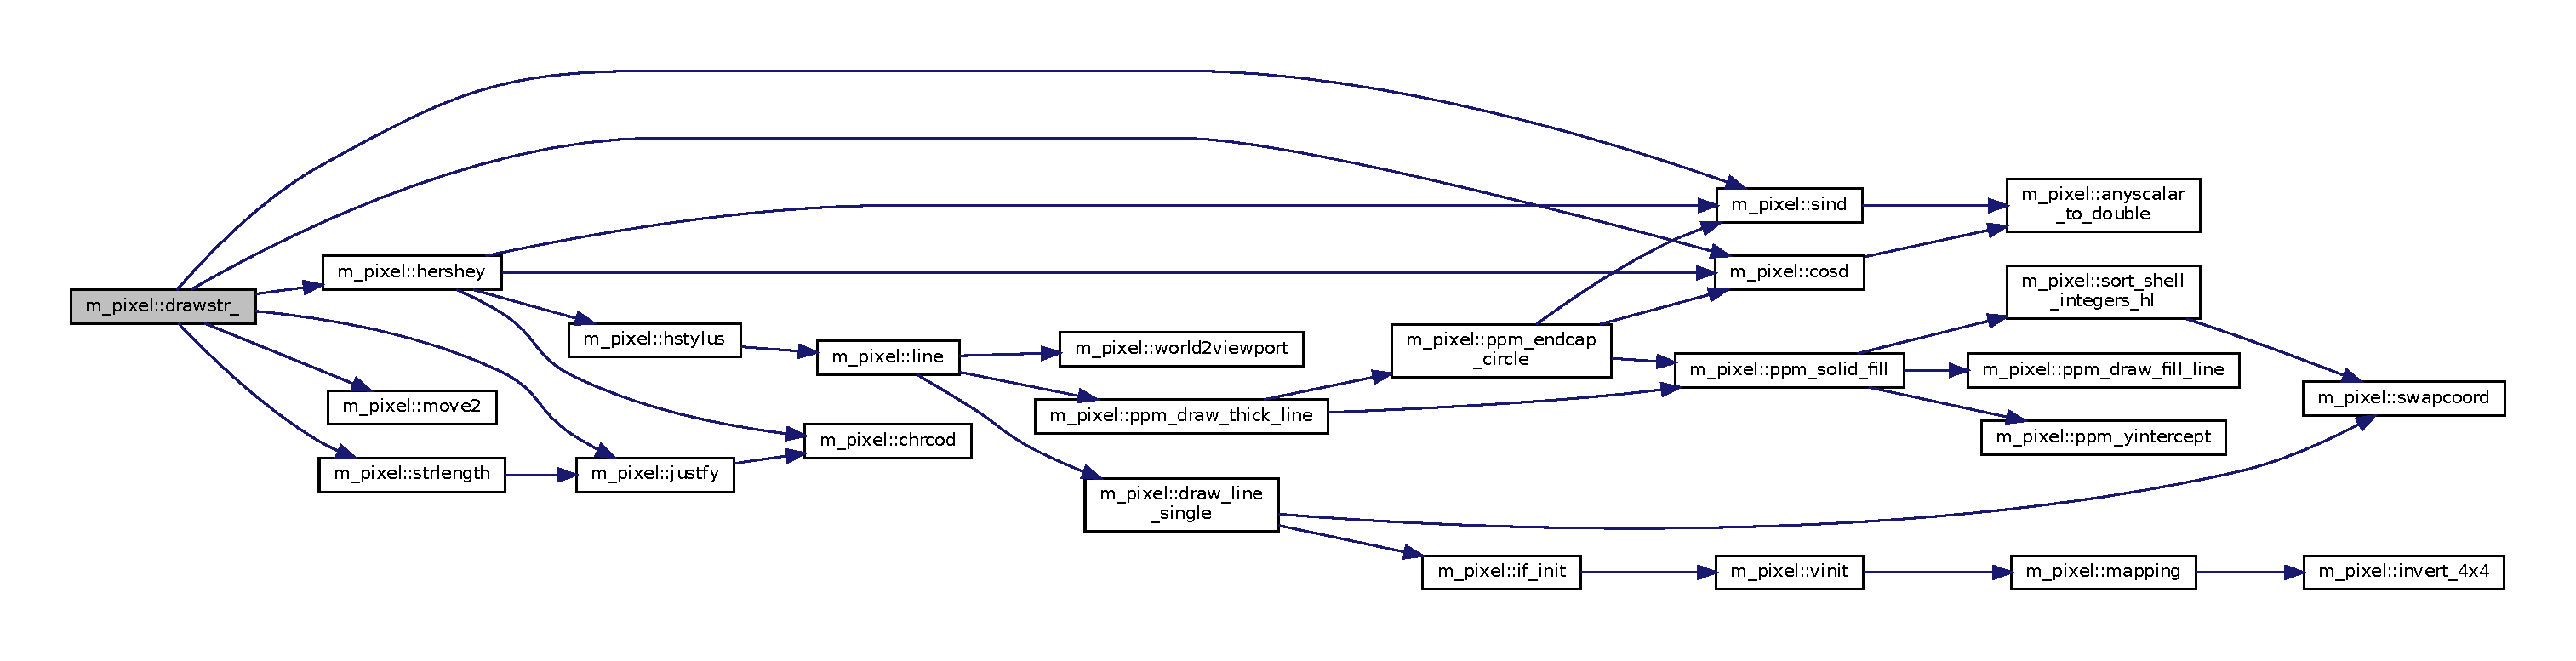
\includegraphics[width=350pt]{namespacem__pixel_a3f8850328e359af5802954b2f70652f5_cgraph}
\end{center}
\end{figure}
Here is the caller graph for this function\+:
\nopagebreak
\begin{figure}[H]
\begin{center}
\leavevmode
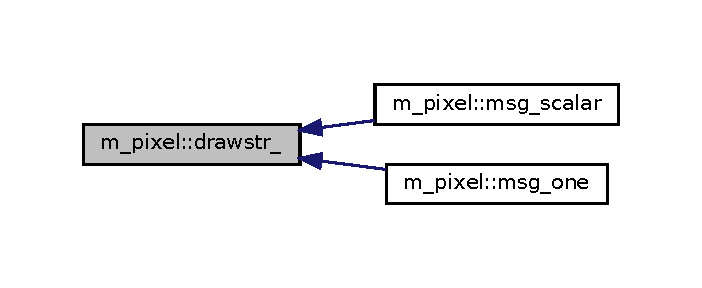
\includegraphics[width=337pt]{namespacem__pixel_a3f8850328e359af5802954b2f70652f5_icgraph}
\end{center}
\end{figure}
\mbox{\Hypertarget{namespacem__pixel_a566adb827a3a26ba42d4e86e4c6e12af}\label{namespacem__pixel_a566adb827a3a26ba42d4e86e4c6e12af}} 
\index{m\+\_\+pixel@{m\+\_\+pixel}!font@{font}}
\index{font@{font}!m\+\_\+pixel@{m\+\_\+pixel}}
\subsubsection{\texorpdfstring{font()}{font()}}
{\footnotesize\ttfamily subroutine, public m\+\_\+pixel\+::font (\begin{DoxyParamCaption}\item[{character(len=$\ast$), intent(in)}]{fontname }\end{DoxyParamCaption})}



References p\+\_\+font.

\mbox{\Hypertarget{namespacem__pixel_acacbc4462423b9aa0f591cbe7aba4ec6}\label{namespacem__pixel_acacbc4462423b9aa0f591cbe7aba4ec6}} 
\index{m\+\_\+pixel@{m\+\_\+pixel}!getdisplaysize@{getdisplaysize}}
\index{getdisplaysize@{getdisplaysize}!m\+\_\+pixel@{m\+\_\+pixel}}
\subsubsection{\texorpdfstring{getdisplaysize()}{getdisplaysize()}}
{\footnotesize\ttfamily subroutine, public m\+\_\+pixel\+::getdisplaysize (\begin{DoxyParamCaption}\item[{real, intent(out)}]{w,  }\item[{real, intent(out)}]{h }\end{DoxyParamCaption})}



References p\+\_\+viewport\+\_\+height, and p\+\_\+viewport\+\_\+width.

Here is the caller graph for this function\+:
\nopagebreak
\begin{figure}[H]
\begin{center}
\leavevmode
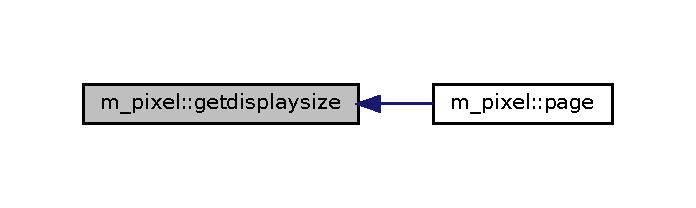
\includegraphics[width=350pt]{namespacem__pixel_acacbc4462423b9aa0f591cbe7aba4ec6_icgraph}
\end{center}
\end{figure}
\mbox{\Hypertarget{namespacem__pixel_a626d769d3dae0c292e3ef1617ad43efb}\label{namespacem__pixel_a626d769d3dae0c292e3ef1617ad43efb}} 
\index{m\+\_\+pixel@{m\+\_\+pixel}!getgp2@{getgp2}}
\index{getgp2@{getgp2}!m\+\_\+pixel@{m\+\_\+pixel}}
\subsubsection{\texorpdfstring{getgp2()}{getgp2()}}
{\footnotesize\ttfamily subroutine, public m\+\_\+pixel\+::getgp2 (\begin{DoxyParamCaption}\item[{real, intent(out)}]{x,  }\item[{real, intent(out)}]{y }\end{DoxyParamCaption})}



References p\+\_\+x, and p\+\_\+y.

\mbox{\Hypertarget{namespacem__pixel_a9f382cf8d3b69e11d1fdd2f2a4f59dea}\label{namespacem__pixel_a9f382cf8d3b69e11d1fdd2f2a4f59dea}} 
\index{m\+\_\+pixel@{m\+\_\+pixel}!getviewport@{getviewport}}
\index{getviewport@{getviewport}!m\+\_\+pixel@{m\+\_\+pixel}}
\subsubsection{\texorpdfstring{getviewport()}{getviewport()}}
{\footnotesize\ttfamily subroutine, public m\+\_\+pixel\+::getviewport (\begin{DoxyParamCaption}\item[{real, intent(out)}]{left,  }\item[{real, intent(out)}]{right,  }\item[{real, intent(out)}]{bottom,  }\item[{real, intent(out)}]{top }\end{DoxyParamCaption})}



References p\+\_\+viewport\+\_\+bottom, p\+\_\+viewport\+\_\+left, p\+\_\+viewport\+\_\+right, and p\+\_\+viewport\+\_\+top.

\mbox{\Hypertarget{namespacem__pixel_a80dc3cb149287470a9837de8dd3f05bc}\label{namespacem__pixel_a80dc3cb149287470a9837de8dd3f05bc}} 
\index{m\+\_\+pixel@{m\+\_\+pixel}!hershey@{hershey}}
\index{hershey@{hershey}!m\+\_\+pixel@{m\+\_\+pixel}}
\subsubsection{\texorpdfstring{hershey()}{hershey()}}
{\footnotesize\ttfamily subroutine, public m\+\_\+pixel\+::hershey (\begin{DoxyParamCaption}\item[{real, intent(in)}]{x,  }\item[{real, intent(in)}]{y,  }\item[{real, intent(in)}]{height,  }\item[{character(len=$\ast$), intent(in)}]{itext,  }\item[{real, intent(in)}]{theta,  }\item[{integer, intent(in)}]{ntext }\end{DoxyParamCaption})}



References chrcod(), cosd(), hstylus(), isstar, istart, p\+\_\+ichr, p\+\_\+ioff, p\+\_\+just1, p\+\_\+just2, p\+\_\+nchr, sind(), ssymbc, symbcd, and width.

Here is the call graph for this function\+:
\nopagebreak
\begin{figure}[H]
\begin{center}
\leavevmode
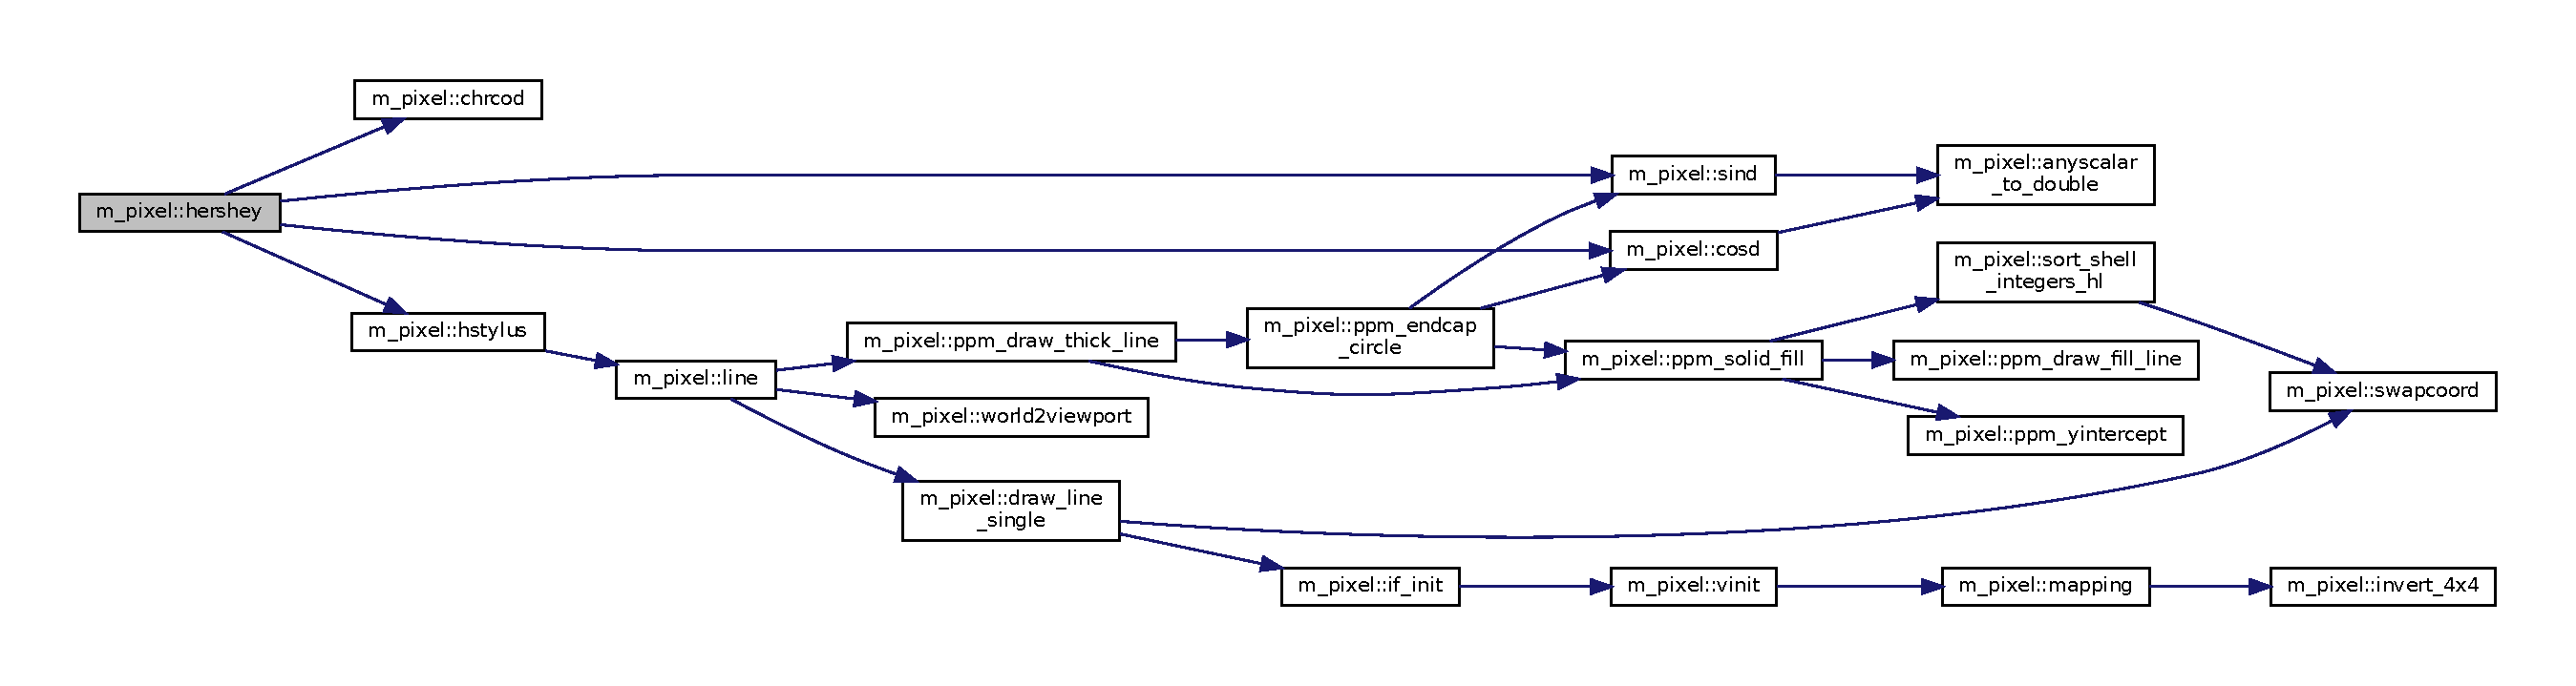
\includegraphics[width=350pt]{namespacem__pixel_a80dc3cb149287470a9837de8dd3f05bc_cgraph}
\end{center}
\end{figure}
Here is the caller graph for this function\+:
\nopagebreak
\begin{figure}[H]
\begin{center}
\leavevmode
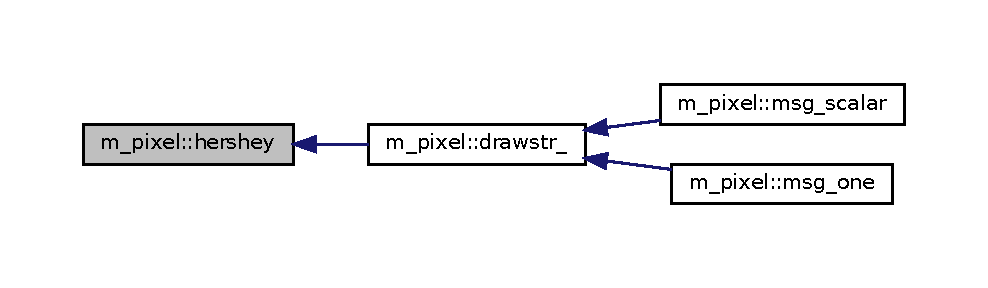
\includegraphics[width=350pt]{namespacem__pixel_a80dc3cb149287470a9837de8dd3f05bc_icgraph}
\end{center}
\end{figure}
\mbox{\Hypertarget{namespacem__pixel_a854b4980c2694d7c33b2830a225eeca0}\label{namespacem__pixel_a854b4980c2694d7c33b2830a225eeca0}} 
\index{m\+\_\+pixel@{m\+\_\+pixel}!hlsrgb@{hlsrgb}}
\index{hlsrgb@{hlsrgb}!m\+\_\+pixel@{m\+\_\+pixel}}
\subsubsection{\texorpdfstring{hlsrgb()}{hlsrgb()}}
{\footnotesize\ttfamily subroutine, private m\+\_\+pixel\+::hlsrgb (\begin{DoxyParamCaption}\item[{real, intent(in)}]{H,  }\item[{real, intent(in)}]{L,  }\item[{real, intent(in)}]{S,  }\item[{real, intent(out)}]{R,  }\item[{real, intent(out)}]{G,  }\item[{real, intent(out)}]{B,  }\item[{integer}]{status }\end{DoxyParamCaption})\hspace{0.3cm}{\ttfamily [private]}}



References hue(), and rgbval().

Here is the call graph for this function\+:
\nopagebreak
\begin{figure}[H]
\begin{center}
\leavevmode
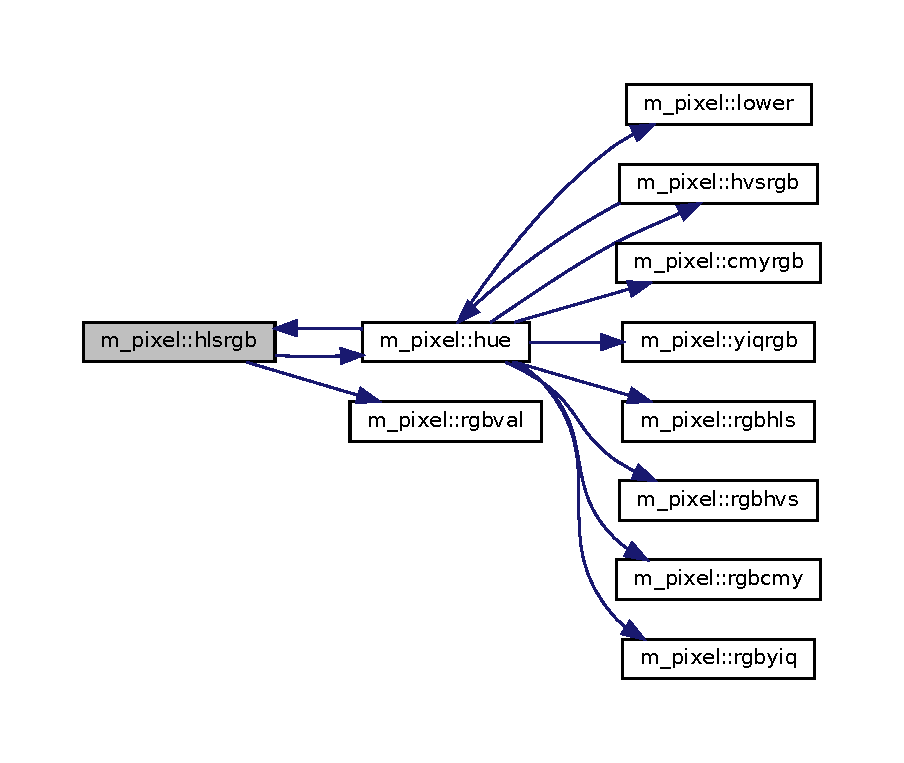
\includegraphics[width=350pt]{namespacem__pixel_a854b4980c2694d7c33b2830a225eeca0_cgraph}
\end{center}
\end{figure}
Here is the caller graph for this function\+:
\nopagebreak
\begin{figure}[H]
\begin{center}
\leavevmode
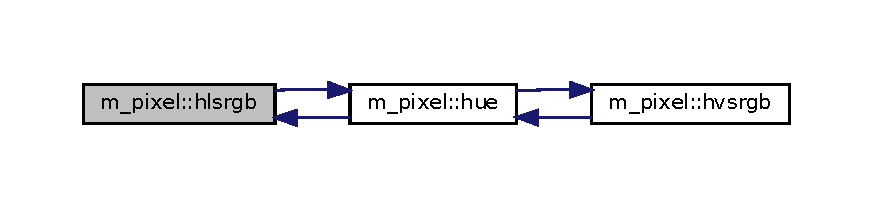
\includegraphics[width=350pt]{namespacem__pixel_a854b4980c2694d7c33b2830a225eeca0_icgraph}
\end{center}
\end{figure}
\mbox{\Hypertarget{namespacem__pixel_a15c5daa9ab477991c2c6e17741cf40eb}\label{namespacem__pixel_a15c5daa9ab477991c2c6e17741cf40eb}} 
\index{m\+\_\+pixel@{m\+\_\+pixel}!hstylus@{hstylus}}
\index{hstylus@{hstylus}!m\+\_\+pixel@{m\+\_\+pixel}}
\subsubsection{\texorpdfstring{hstylus()}{hstylus()}}
{\footnotesize\ttfamily subroutine m\+\_\+pixel\+::hstylus (\begin{DoxyParamCaption}\item[{real, intent(in)}]{xi,  }\item[{real, intent(in)}]{yi,  }\item[{integer, intent(in)}]{ipen }\end{DoxyParamCaption})\hspace{0.3cm}{\ttfamily [private]}}



References line(), p\+\_\+x, and p\+\_\+y.

Here is the call graph for this function\+:
\nopagebreak
\begin{figure}[H]
\begin{center}
\leavevmode
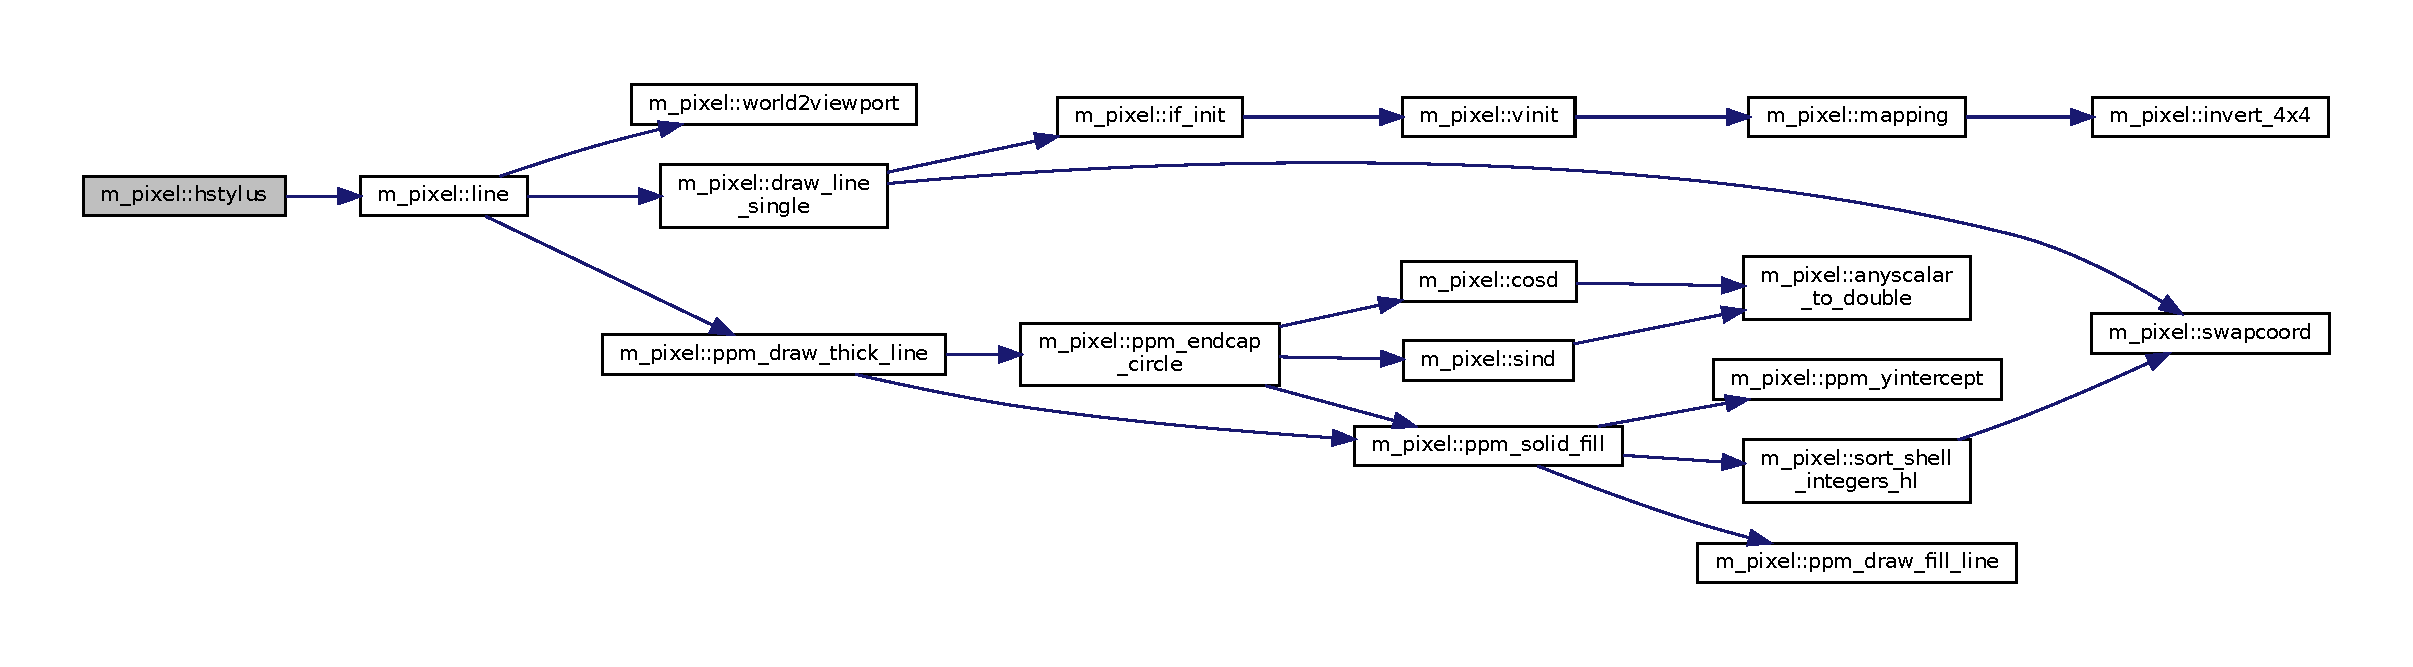
\includegraphics[width=350pt]{namespacem__pixel_a15c5daa9ab477991c2c6e17741cf40eb_cgraph}
\end{center}
\end{figure}
Here is the caller graph for this function\+:
\nopagebreak
\begin{figure}[H]
\begin{center}
\leavevmode
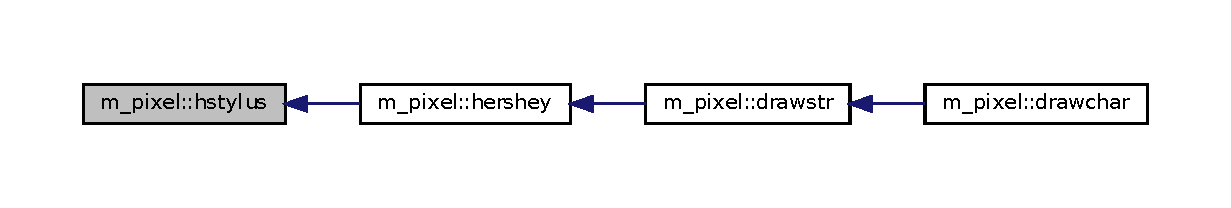
\includegraphics[width=350pt]{namespacem__pixel_a15c5daa9ab477991c2c6e17741cf40eb_icgraph}
\end{center}
\end{figure}
\mbox{\Hypertarget{namespacem__pixel_aa76d2ac385f3ad0bc2b555cc14b7d53f}\label{namespacem__pixel_aa76d2ac385f3ad0bc2b555cc14b7d53f}} 
\index{m\+\_\+pixel@{m\+\_\+pixel}!hue@{hue}}
\index{hue@{hue}!m\+\_\+pixel@{m\+\_\+pixel}}
\subsubsection{\texorpdfstring{hue()}{hue()}}
{\footnotesize\ttfamily subroutine, public m\+\_\+pixel\+::hue (\begin{DoxyParamCaption}\item[{character(len=$\ast$), intent(in)}]{modei,  }\item[{real, intent(in)}]{clr1i,  }\item[{real, intent(in)}]{clr2i,  }\item[{real, intent(in)}]{clr3i,  }\item[{character(len=$\ast$), intent(in)}]{modeo,  }\item[{real, intent(out)}]{clr1o,  }\item[{real, intent(out)}]{clr2o,  }\item[{real, intent(out)}]{clr3o,  }\item[{integer, intent(out)}]{status }\end{DoxyParamCaption})}



References cmyrgb(), hlsrgb(), hvsrgb(), lower(), rgbcmy(), rgbhls(), rgbhvs(), rgbyiq(), and yiqrgb().

Here is the call graph for this function\+:
\nopagebreak
\begin{figure}[H]
\begin{center}
\leavevmode
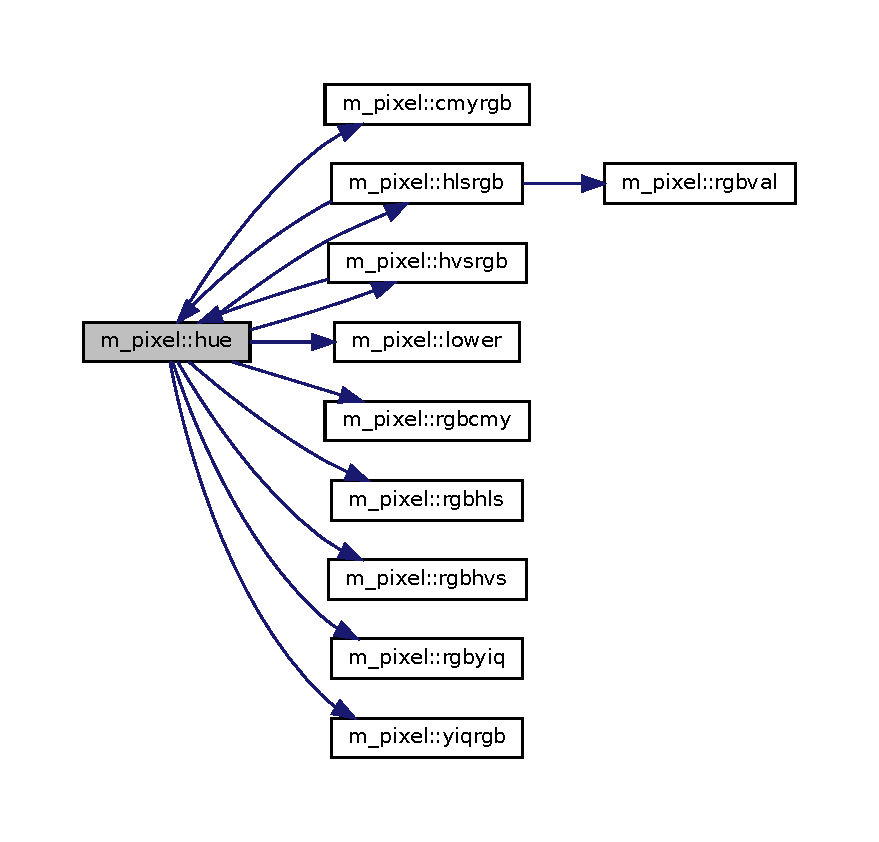
\includegraphics[width=350pt]{namespacem__pixel_aa76d2ac385f3ad0bc2b555cc14b7d53f_cgraph}
\end{center}
\end{figure}
Here is the caller graph for this function\+:
\nopagebreak
\begin{figure}[H]
\begin{center}
\leavevmode
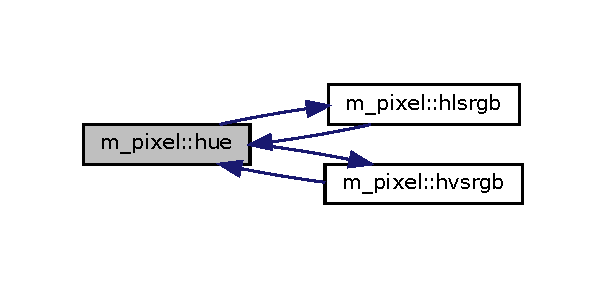
\includegraphics[width=291pt]{namespacem__pixel_aa76d2ac385f3ad0bc2b555cc14b7d53f_icgraph}
\end{center}
\end{figure}
\mbox{\Hypertarget{namespacem__pixel_a6eda5641d5c42b51d9488bd7ea743744}\label{namespacem__pixel_a6eda5641d5c42b51d9488bd7ea743744}} 
\index{m\+\_\+pixel@{m\+\_\+pixel}!hvsrgb@{hvsrgb}}
\index{hvsrgb@{hvsrgb}!m\+\_\+pixel@{m\+\_\+pixel}}
\subsubsection{\texorpdfstring{hvsrgb()}{hvsrgb()}}
{\footnotesize\ttfamily subroutine, private m\+\_\+pixel\+::hvsrgb (\begin{DoxyParamCaption}\item[{real, intent(in)}]{h,  }\item[{real, intent(in)}]{v,  }\item[{real, intent(in)}]{s,  }\item[{real, intent(out)}]{r,  }\item[{real, intent(out)}]{g,  }\item[{real, intent(out)}]{b,  }\item[{integer}]{status }\end{DoxyParamCaption})\hspace{0.3cm}{\ttfamily [private]}}



References hue().

Here is the call graph for this function\+:
\nopagebreak
\begin{figure}[H]
\begin{center}
\leavevmode
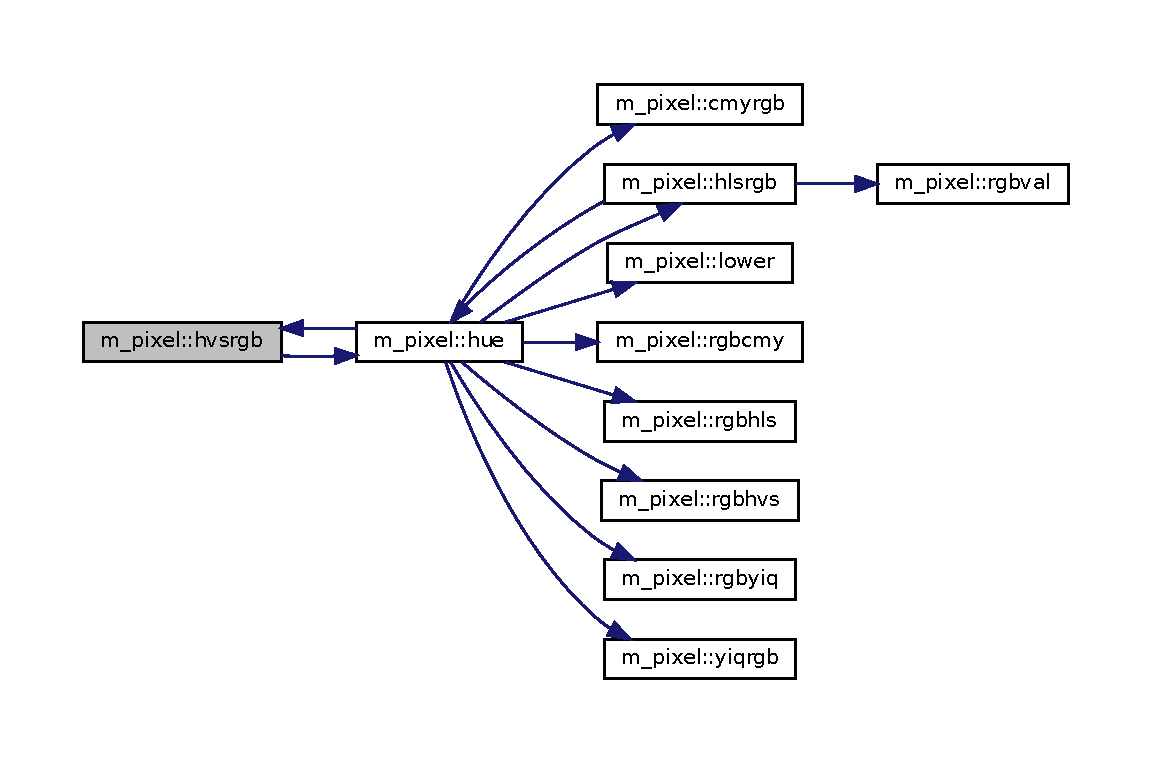
\includegraphics[width=350pt]{namespacem__pixel_a6eda5641d5c42b51d9488bd7ea743744_cgraph}
\end{center}
\end{figure}
Here is the caller graph for this function\+:
\nopagebreak
\begin{figure}[H]
\begin{center}
\leavevmode
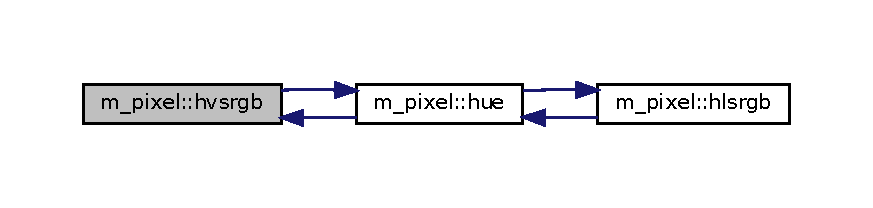
\includegraphics[width=350pt]{namespacem__pixel_a6eda5641d5c42b51d9488bd7ea743744_icgraph}
\end{center}
\end{figure}
\mbox{\Hypertarget{namespacem__pixel_a4d23e0d3f4de5b3652a4eb5a61d7dc8d}\label{namespacem__pixel_a4d23e0d3f4de5b3652a4eb5a61d7dc8d}} 
\index{m\+\_\+pixel@{m\+\_\+pixel}!i2s@{i2s}}
\index{i2s@{i2s}!m\+\_\+pixel@{m\+\_\+pixel}}
\subsubsection{\texorpdfstring{i2s()}{i2s()}}
{\footnotesize\ttfamily character(len=\+:) function, allocatable, public m\+\_\+pixel\+::i2s (\begin{DoxyParamCaption}\item[{integer, intent(in)}]{ivalue }\end{DoxyParamCaption})}

Here is the caller graph for this function\+:
\nopagebreak
\begin{figure}[H]
\begin{center}
\leavevmode
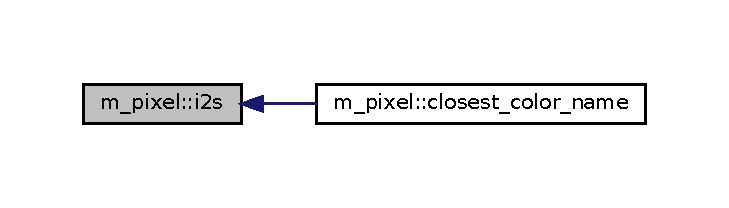
\includegraphics[width=350pt]{namespacem__pixel_a4d23e0d3f4de5b3652a4eb5a61d7dc8d_icgraph}
\end{center}
\end{figure}
\mbox{\Hypertarget{namespacem__pixel_a6c23c2779e54da4ac7505cfb816cc2b1}\label{namespacem__pixel_a6c23c2779e54da4ac7505cfb816cc2b1}} 
\index{m\+\_\+pixel@{m\+\_\+pixel}!if\+\_\+init@{if\+\_\+init}}
\index{if\+\_\+init@{if\+\_\+init}!m\+\_\+pixel@{m\+\_\+pixel}}
\subsubsection{\texorpdfstring{if\+\_\+init()}{if\_init()}}
{\footnotesize\ttfamily subroutine m\+\_\+pixel\+::if\+\_\+init (\begin{DoxyParamCaption}{ }\end{DoxyParamCaption})\hspace{0.3cm}{\ttfamily [private]}}



References p\+\_\+vinit\+\_\+called, and vinit().

Here is the call graph for this function\+:
\nopagebreak
\begin{figure}[H]
\begin{center}
\leavevmode
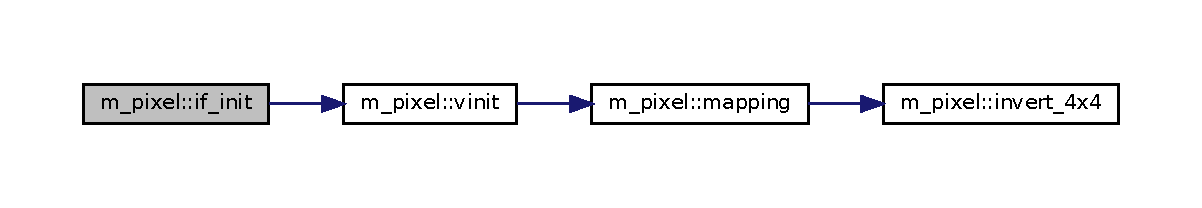
\includegraphics[width=350pt]{namespacem__pixel_a6c23c2779e54da4ac7505cfb816cc2b1_cgraph}
\end{center}
\end{figure}
Here is the caller graph for this function\+:
\nopagebreak
\begin{figure}[H]
\begin{center}
\leavevmode
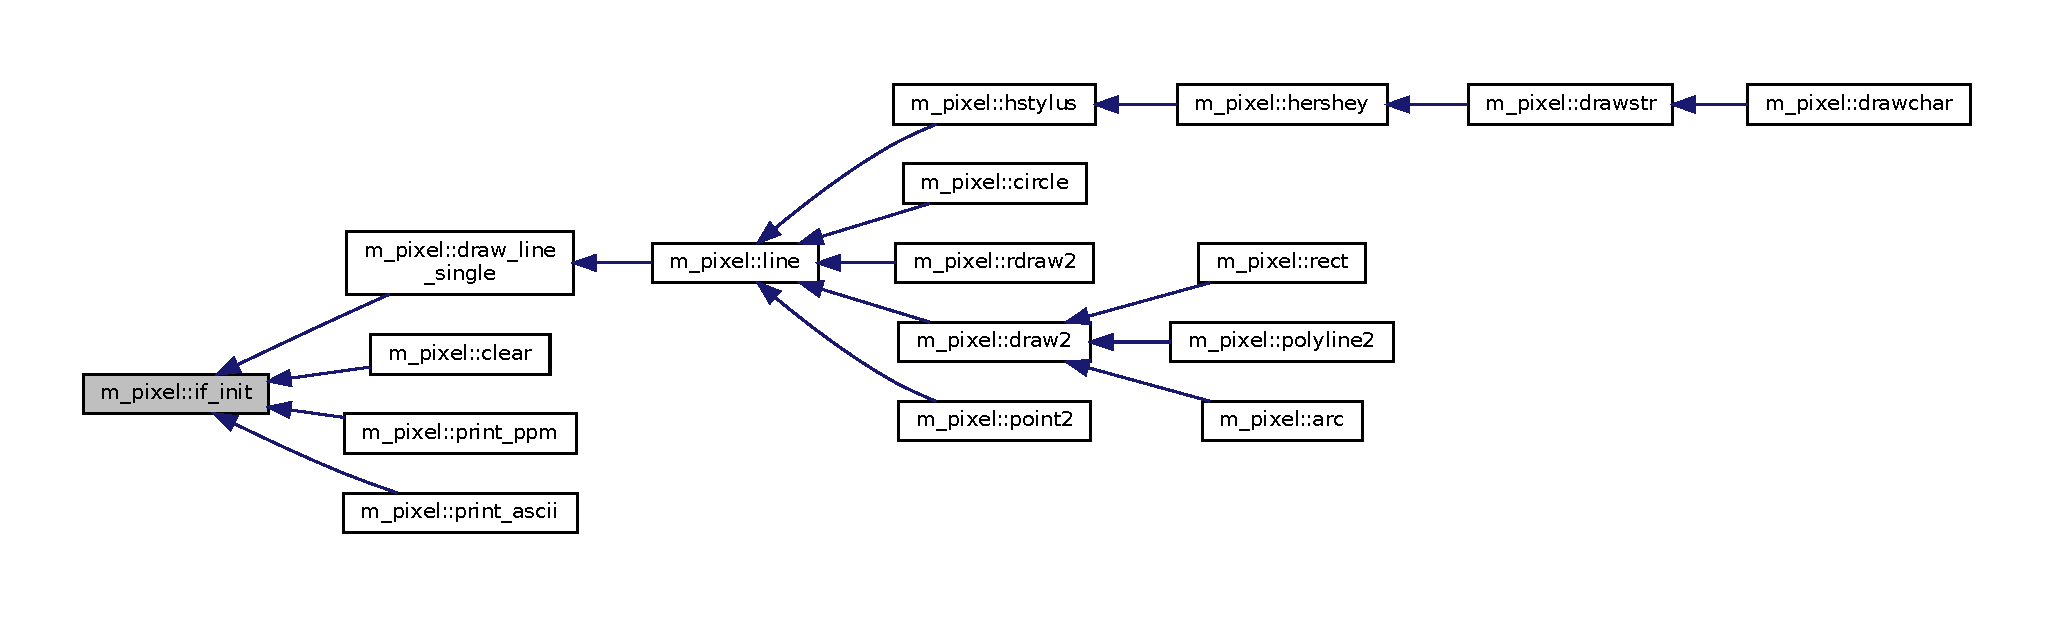
\includegraphics[width=350pt]{namespacem__pixel_a6c23c2779e54da4ac7505cfb816cc2b1_icgraph}
\end{center}
\end{figure}
\mbox{\Hypertarget{namespacem__pixel_a630b892544962a88d91b1ab983dc5649}\label{namespacem__pixel_a630b892544962a88d91b1ab983dc5649}} 
\index{m\+\_\+pixel@{m\+\_\+pixel}!invert\+\_\+4x4@{invert\+\_\+4x4}}
\index{invert\+\_\+4x4@{invert\+\_\+4x4}!m\+\_\+pixel@{m\+\_\+pixel}}
\subsubsection{\texorpdfstring{invert\+\_\+4x4()}{invert\_4x4()}}
{\footnotesize\ttfamily pure real(kind=wp) function, dimension(4,4) m\+\_\+pixel\+::invert\+\_\+4x4 (\begin{DoxyParamCaption}\item[{real(kind=wp), dimension(4,4), intent(in)}]{A }\end{DoxyParamCaption})\hspace{0.3cm}{\ttfamily [private]}}

Here is the caller graph for this function\+:
\nopagebreak
\begin{figure}[H]
\begin{center}
\leavevmode
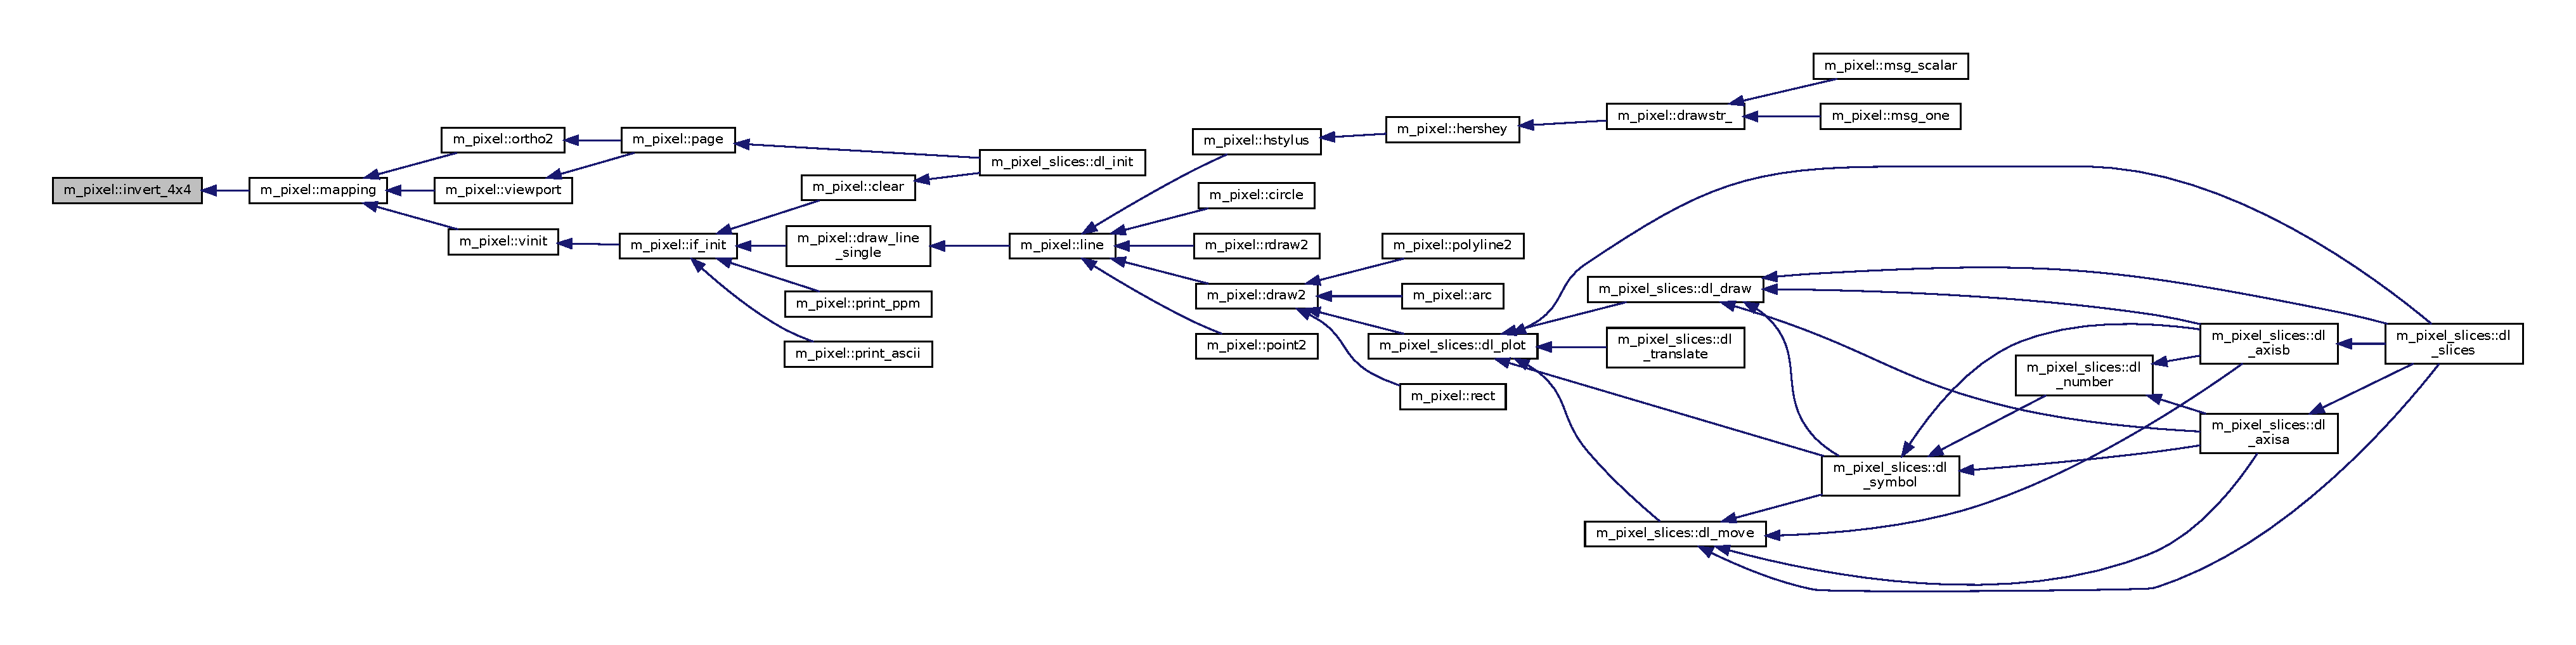
\includegraphics[width=350pt]{namespacem__pixel_a630b892544962a88d91b1ab983dc5649_icgraph}
\end{center}
\end{figure}
\mbox{\Hypertarget{namespacem__pixel_ac39c9efa849915aff58657e2df03fe3c}\label{namespacem__pixel_ac39c9efa849915aff58657e2df03fe3c}} 
\index{m\+\_\+pixel@{m\+\_\+pixel}!journal@{journal}}
\index{journal@{journal}!m\+\_\+pixel@{m\+\_\+pixel}}
\subsubsection{\texorpdfstring{journal()}{journal()}}
{\footnotesize\ttfamily subroutine m\+\_\+pixel\+::journal (\begin{DoxyParamCaption}\item[{character(len=$\ast$), intent(in)}]{string }\end{DoxyParamCaption})\hspace{0.3cm}{\ttfamily [private]}}

Here is the caller graph for this function\+:
\nopagebreak
\begin{figure}[H]
\begin{center}
\leavevmode
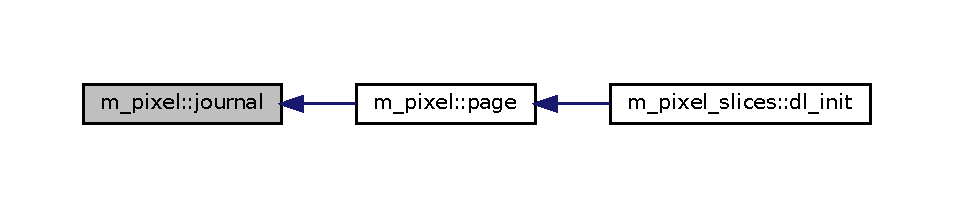
\includegraphics[width=350pt]{namespacem__pixel_ac39c9efa849915aff58657e2df03fe3c_icgraph}
\end{center}
\end{figure}
\mbox{\Hypertarget{namespacem__pixel_a7b08886c913b47694edeb60fa747afc4}\label{namespacem__pixel_a7b08886c913b47694edeb60fa747afc4}} 
\index{m\+\_\+pixel@{m\+\_\+pixel}!justfy@{justfy}}
\index{justfy@{justfy}!m\+\_\+pixel@{m\+\_\+pixel}}
\subsubsection{\texorpdfstring{justfy()}{justfy()}}
{\footnotesize\ttfamily subroutine, public m\+\_\+pixel\+::justfy (\begin{DoxyParamCaption}\item[{real, dimension(4), intent(out)}]{s,  }\item[{real, intent(in)}]{height,  }\item[{character(len=$\ast$), intent(in)}]{text,  }\item[{integer, intent(in)}]{ntext }\end{DoxyParamCaption})}



References chrcod(), p\+\_\+ichr, p\+\_\+just2, p\+\_\+nchr, and width.

Here is the call graph for this function\+:
\nopagebreak
\begin{figure}[H]
\begin{center}
\leavevmode
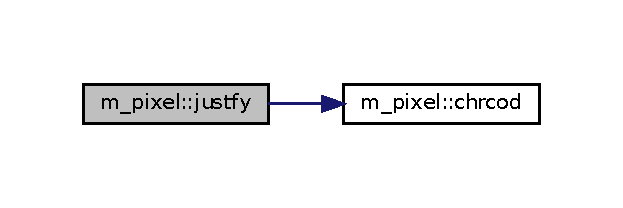
\includegraphics[width=299pt]{namespacem__pixel_a7b08886c913b47694edeb60fa747afc4_cgraph}
\end{center}
\end{figure}
Here is the caller graph for this function\+:
\nopagebreak
\begin{figure}[H]
\begin{center}
\leavevmode
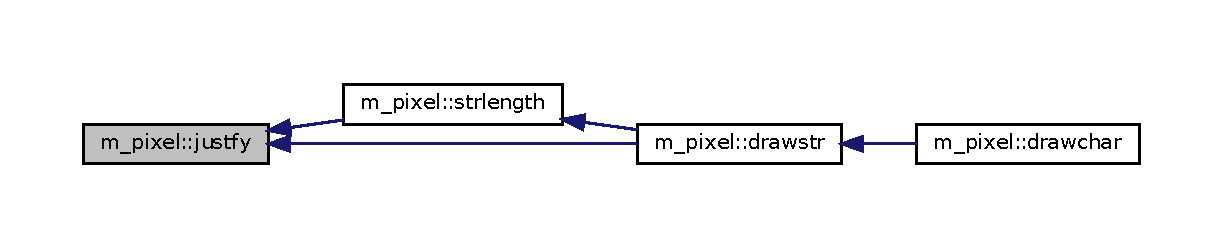
\includegraphics[width=350pt]{namespacem__pixel_a7b08886c913b47694edeb60fa747afc4_icgraph}
\end{center}
\end{figure}
\mbox{\Hypertarget{namespacem__pixel_a491951b89e60d0d40d67f22d987da894}\label{namespacem__pixel_a491951b89e60d0d40d67f22d987da894}} 
\index{m\+\_\+pixel@{m\+\_\+pixel}!line@{line}}
\index{line@{line}!m\+\_\+pixel@{m\+\_\+pixel}}
\subsubsection{\texorpdfstring{line()}{line()}}
{\footnotesize\ttfamily subroutine, public m\+\_\+pixel\+::line (\begin{DoxyParamCaption}\item[{real, intent(in)}]{x1,  }\item[{real, intent(in)}]{y1,  }\item[{real, intent(in)}]{x2,  }\item[{real, intent(in)}]{y2 }\end{DoxyParamCaption})}



References draw\+\_\+line\+\_\+single(), p\+\_\+debug, p\+\_\+inpolygon, p\+\_\+maxverts, p\+\_\+polypoints, p\+\_\+polyvertex, p\+\_\+width, p\+\_\+x, p\+\_\+y, ppm\+\_\+draw\+\_\+thick\+\_\+line(), and world2viewport().

Here is the call graph for this function\+:
\nopagebreak
\begin{figure}[H]
\begin{center}
\leavevmode
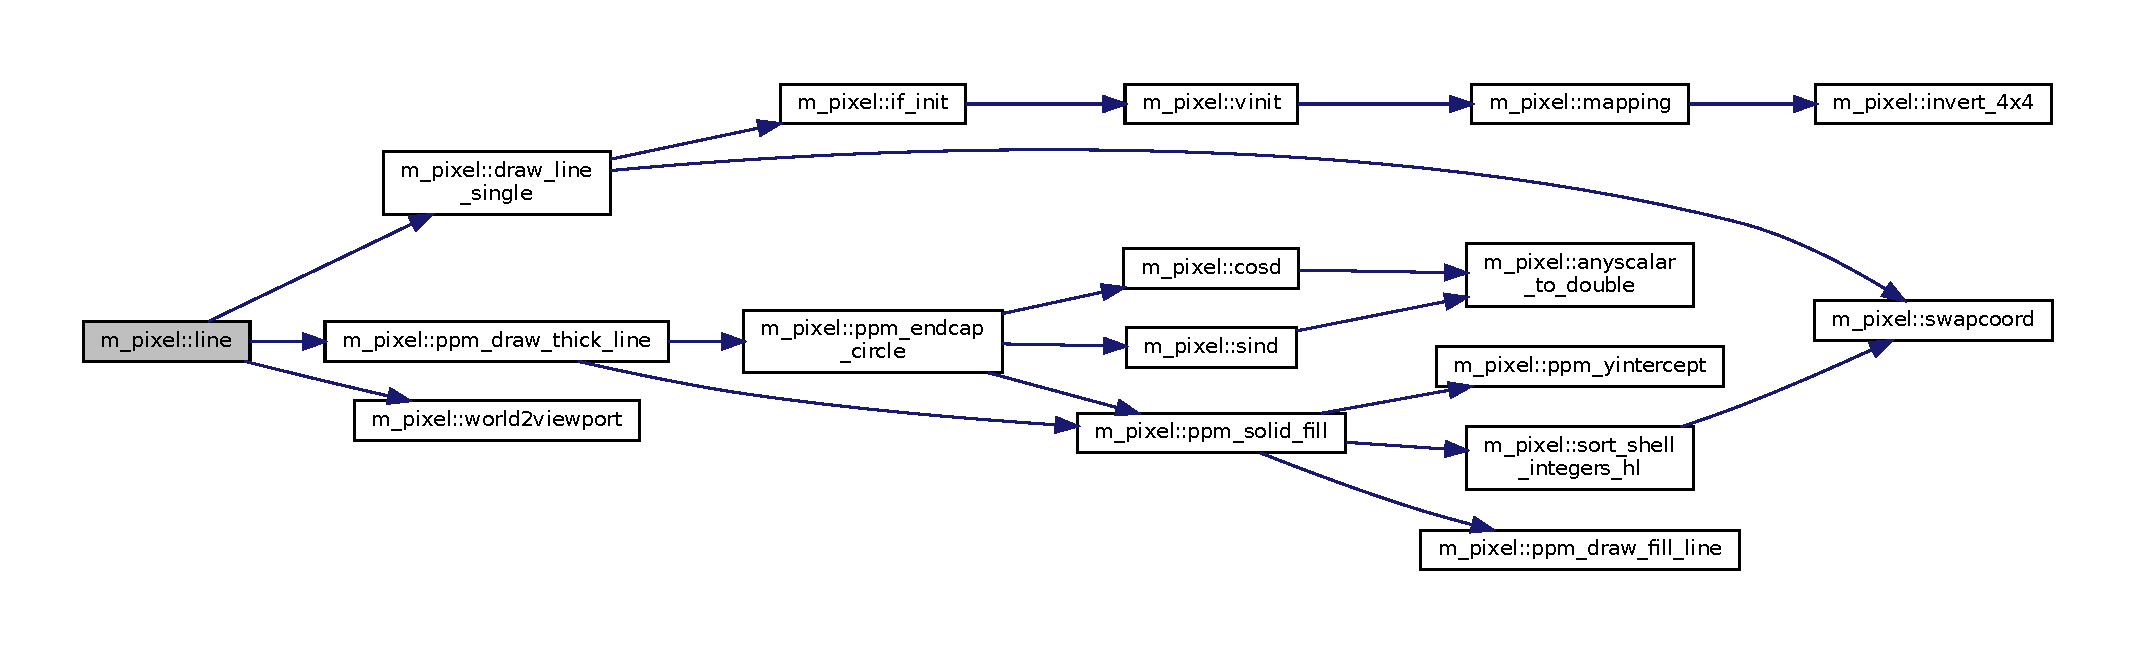
\includegraphics[width=350pt]{namespacem__pixel_a491951b89e60d0d40d67f22d987da894_cgraph}
\end{center}
\end{figure}
Here is the caller graph for this function\+:
\nopagebreak
\begin{figure}[H]
\begin{center}
\leavevmode
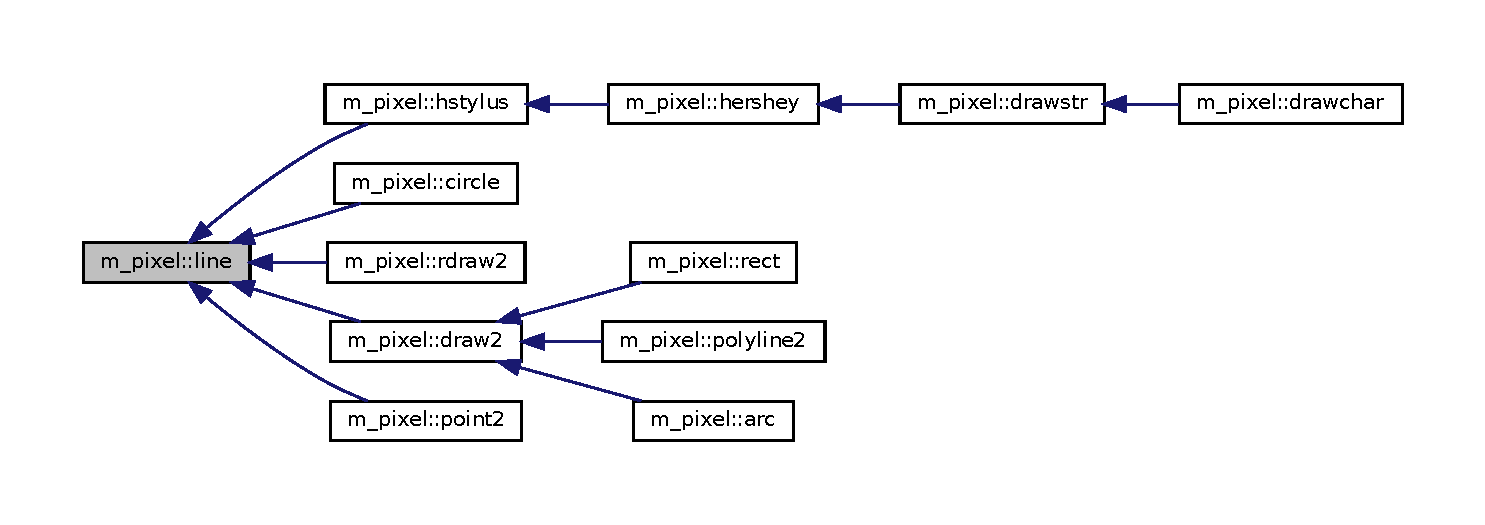
\includegraphics[width=350pt]{namespacem__pixel_a491951b89e60d0d40d67f22d987da894_icgraph}
\end{center}
\end{figure}
\mbox{\Hypertarget{namespacem__pixel_a16379e283aaa99e2e0ba1eb26e93452d}\label{namespacem__pixel_a16379e283aaa99e2e0ba1eb26e93452d}} 
\index{m\+\_\+pixel@{m\+\_\+pixel}!linewidth@{linewidth}}
\index{linewidth@{linewidth}!m\+\_\+pixel@{m\+\_\+pixel}}
\subsubsection{\texorpdfstring{linewidth()}{linewidth()}}
{\footnotesize\ttfamily subroutine, public m\+\_\+pixel\+::linewidth (\begin{DoxyParamCaption}\item[{integer, intent(in)}]{iwidth }\end{DoxyParamCaption})}



References p\+\_\+viewport\+\_\+width, and p\+\_\+width.

Here is the caller graph for this function\+:
\nopagebreak
\begin{figure}[H]
\begin{center}
\leavevmode
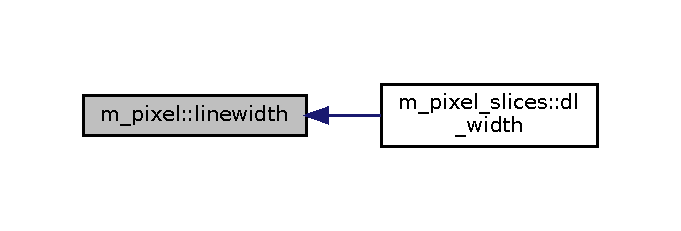
\includegraphics[width=327pt]{namespacem__pixel_a16379e283aaa99e2e0ba1eb26e93452d_icgraph}
\end{center}
\end{figure}
\mbox{\Hypertarget{namespacem__pixel_a7b4934756a8325a19fee6653c4cbf6af}\label{namespacem__pixel_a7b4934756a8325a19fee6653c4cbf6af}} 
\index{m\+\_\+pixel@{m\+\_\+pixel}!lower@{lower}}
\index{lower@{lower}!m\+\_\+pixel@{m\+\_\+pixel}}
\subsubsection{\texorpdfstring{lower()}{lower()}}
{\footnotesize\ttfamily elemental pure character(len(str)) function, public m\+\_\+pixel\+::lower (\begin{DoxyParamCaption}\item[{character($\ast$), intent(in)}]{str }\end{DoxyParamCaption})}

Here is the caller graph for this function\+:
\nopagebreak
\begin{figure}[H]
\begin{center}
\leavevmode
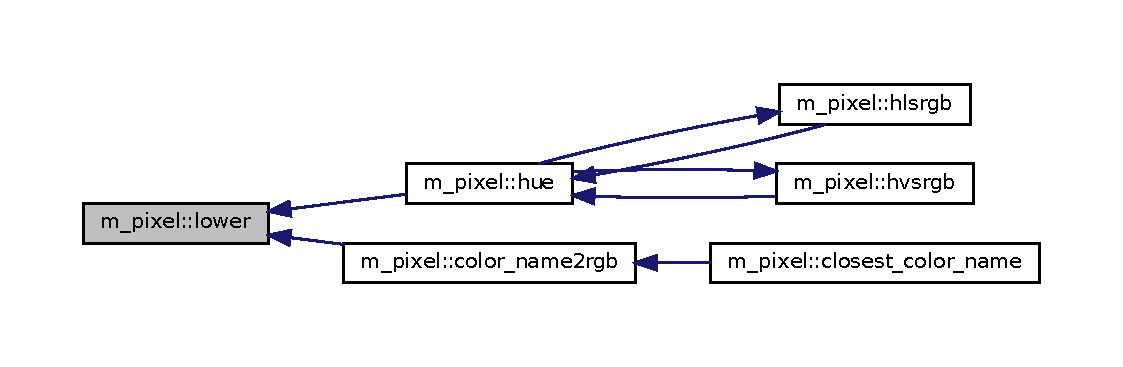
\includegraphics[width=350pt]{namespacem__pixel_a7b4934756a8325a19fee6653c4cbf6af_icgraph}
\end{center}
\end{figure}
\mbox{\Hypertarget{namespacem__pixel_ab7128437f95b40004bf73fc6e3f597f8}\label{namespacem__pixel_ab7128437f95b40004bf73fc6e3f597f8}} 
\index{m\+\_\+pixel@{m\+\_\+pixel}!makepoly@{makepoly}}
\index{makepoly@{makepoly}!m\+\_\+pixel@{m\+\_\+pixel}}
\subsubsection{\texorpdfstring{makepoly()}{makepoly()}}
{\footnotesize\ttfamily subroutine, public m\+\_\+pixel\+::makepoly (\begin{DoxyParamCaption}{ }\end{DoxyParamCaption})}



References p\+\_\+inpolygon, and p\+\_\+polyvertex.

\mbox{\Hypertarget{namespacem__pixel_a3422f51171f30979868a8075690da9f5}\label{namespacem__pixel_a3422f51171f30979868a8075690da9f5}} 
\index{m\+\_\+pixel@{m\+\_\+pixel}!mapcolor@{mapcolor}}
\index{mapcolor@{mapcolor}!m\+\_\+pixel@{m\+\_\+pixel}}
\subsubsection{\texorpdfstring{mapcolor()}{mapcolor()}}
{\footnotesize\ttfamily subroutine, public m\+\_\+pixel\+::mapcolor (\begin{DoxyParamCaption}\item[{integer, intent(in)}]{indx,  }\item[{integer, intent(in)}]{red,  }\item[{integer, intent(in)}]{green,  }\item[{integer, intent(in)}]{blue }\end{DoxyParamCaption})}



References p\+\_\+colormap.

\mbox{\Hypertarget{namespacem__pixel_a84c841de62fc0addddeff305c4ede9d4}\label{namespacem__pixel_a84c841de62fc0addddeff305c4ede9d4}} 
\index{m\+\_\+pixel@{m\+\_\+pixel}!mapping@{mapping}}
\index{mapping@{mapping}!m\+\_\+pixel@{m\+\_\+pixel}}
\subsubsection{\texorpdfstring{mapping()}{mapping()}}
{\footnotesize\ttfamily subroutine m\+\_\+pixel\+::mapping (\begin{DoxyParamCaption}{ }\end{DoxyParamCaption})\hspace{0.3cm}{\ttfamily [private]}}



References invert\+\_\+4x4(), p\+\_\+a, p\+\_\+b, p\+\_\+c, p\+\_\+d, p\+\_\+viewport\+\_\+bottom, p\+\_\+viewport\+\_\+left, p\+\_\+viewport\+\_\+right, p\+\_\+viewport\+\_\+top, p\+\_\+window\+\_\+bottom, p\+\_\+window\+\_\+left, p\+\_\+window\+\_\+right, and p\+\_\+window\+\_\+top.

Here is the call graph for this function\+:
\nopagebreak
\begin{figure}[H]
\begin{center}
\leavevmode
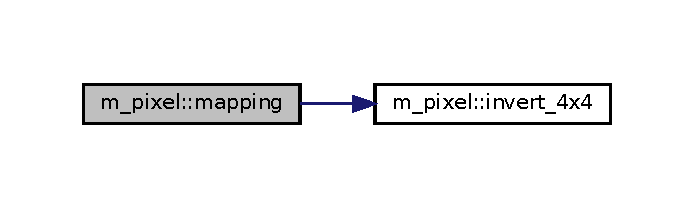
\includegraphics[width=333pt]{namespacem__pixel_a84c841de62fc0addddeff305c4ede9d4_cgraph}
\end{center}
\end{figure}
Here is the caller graph for this function\+:
\nopagebreak
\begin{figure}[H]
\begin{center}
\leavevmode
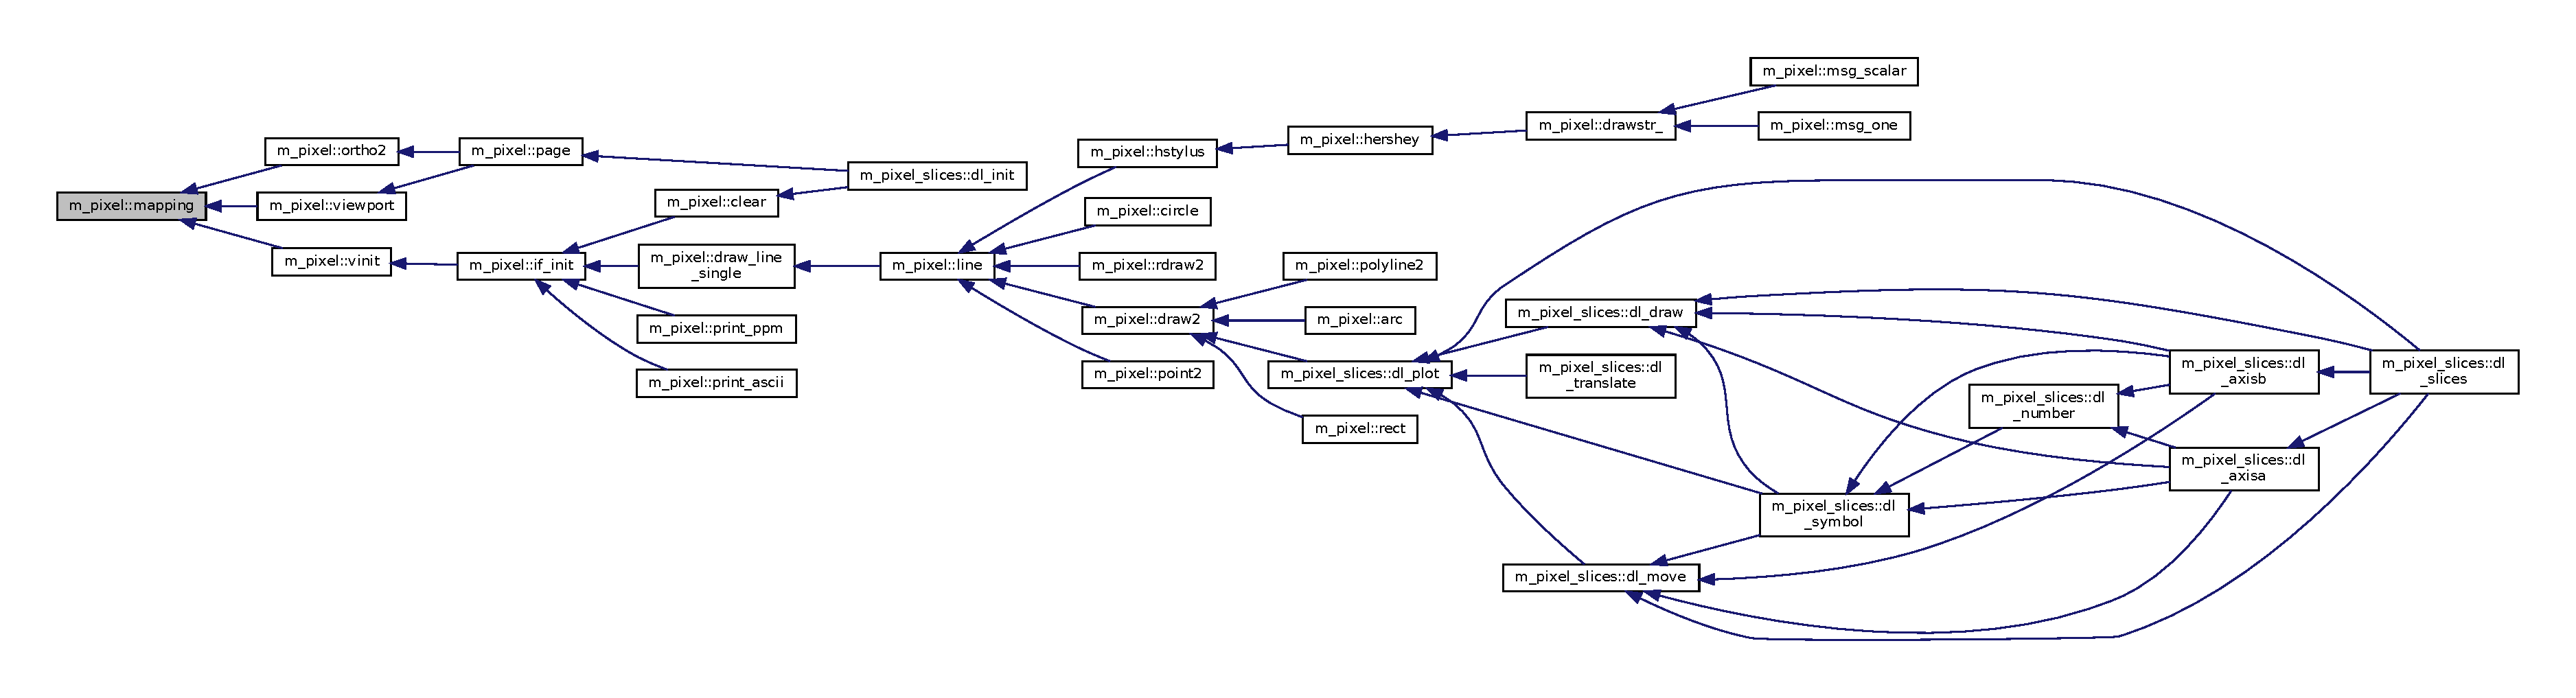
\includegraphics[width=350pt]{namespacem__pixel_a84c841de62fc0addddeff305c4ede9d4_icgraph}
\end{center}
\end{figure}
\mbox{\Hypertarget{namespacem__pixel_ab5d4dc474ff84dc0f3f35f4a395979e0}\label{namespacem__pixel_ab5d4dc474ff84dc0f3f35f4a395979e0}} 
\index{m\+\_\+pixel@{m\+\_\+pixel}!move2@{move2}}
\index{move2@{move2}!m\+\_\+pixel@{m\+\_\+pixel}}
\subsubsection{\texorpdfstring{move2()}{move2()}}
{\footnotesize\ttfamily subroutine, public m\+\_\+pixel\+::move2 (\begin{DoxyParamCaption}\item[{real, intent(in)}]{x,  }\item[{real, intent(in)}]{y }\end{DoxyParamCaption})}



References p\+\_\+x, and p\+\_\+y.

Here is the caller graph for this function\+:
\nopagebreak
\begin{figure}[H]
\begin{center}
\leavevmode
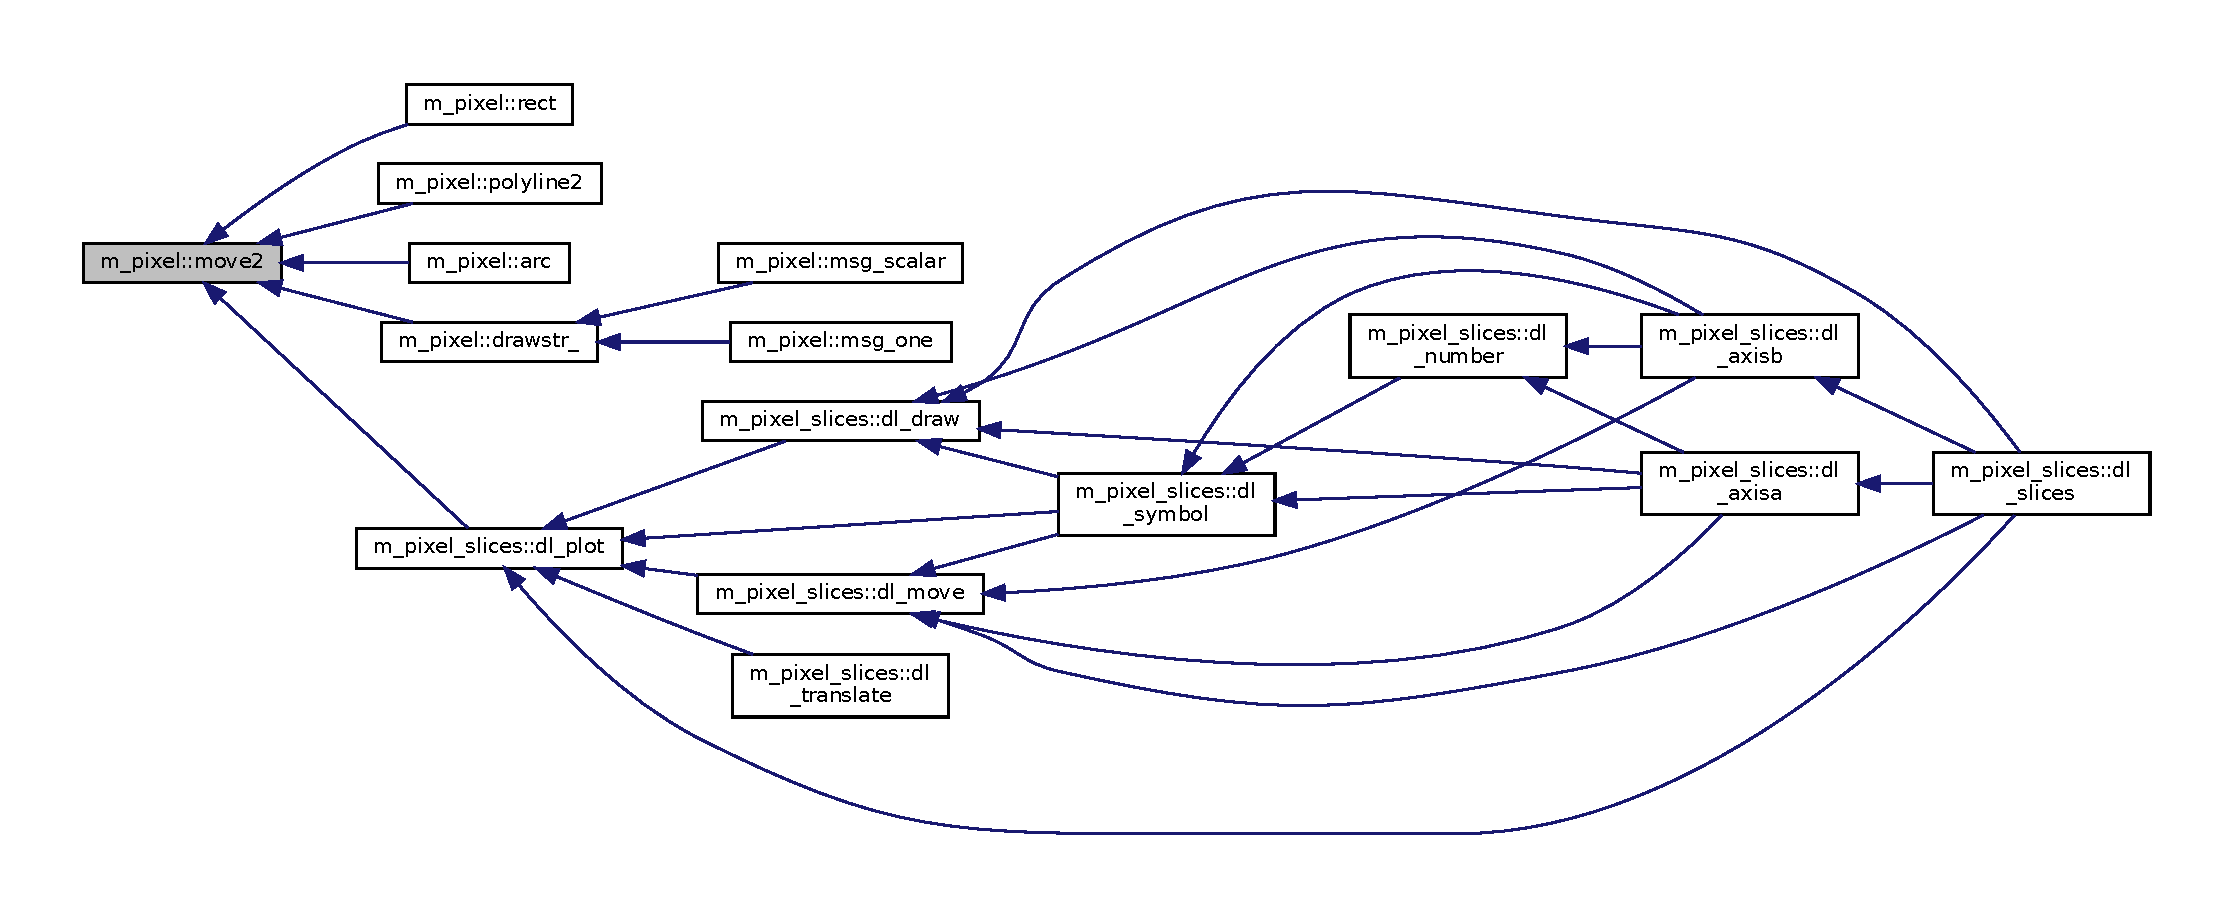
\includegraphics[width=350pt]{namespacem__pixel_ab5d4dc474ff84dc0f3f35f4a395979e0_icgraph}
\end{center}
\end{figure}
\mbox{\Hypertarget{namespacem__pixel_a8c097c521deafffc765bd3f35eca423c}\label{namespacem__pixel_a8c097c521deafffc765bd3f35eca423c}} 
\index{m\+\_\+pixel@{m\+\_\+pixel}!msg\+\_\+one@{msg\+\_\+one}}
\index{msg\+\_\+one@{msg\+\_\+one}!m\+\_\+pixel@{m\+\_\+pixel}}
\subsubsection{\texorpdfstring{msg\+\_\+one()}{msg\_one()}}
{\footnotesize\ttfamily subroutine m\+\_\+pixel\+::msg\+\_\+one (\begin{DoxyParamCaption}\item[{class($\ast$), dimension(\+:), intent(in)}]{generic0,  }\item[{class($\ast$), dimension(\+:), intent(in), optional}]{generic1,  }\item[{class($\ast$), dimension(\+:), intent(in), optional}]{generic2,  }\item[{class($\ast$), dimension(\+:), intent(in), optional}]{generic3,  }\item[{class($\ast$), dimension(\+:), intent(in), optional}]{generic4,  }\item[{class($\ast$), dimension(\+:), intent(in), optional}]{generic5,  }\item[{class($\ast$), dimension(\+:), intent(in), optional}]{generic6,  }\item[{class($\ast$), dimension(\+:), intent(in), optional}]{generic7,  }\item[{class($\ast$), dimension(\+:), intent(in), optional}]{generic8,  }\item[{class($\ast$), dimension(\+:), intent(in), optional}]{generic9,  }\item[{logical, intent(in), optional}]{nospace }\end{DoxyParamCaption})\hspace{0.3cm}{\ttfamily [private]}}



References drawstr\+\_\+(), and print\+\_\+generic().

Here is the call graph for this function\+:
\nopagebreak
\begin{figure}[H]
\begin{center}
\leavevmode
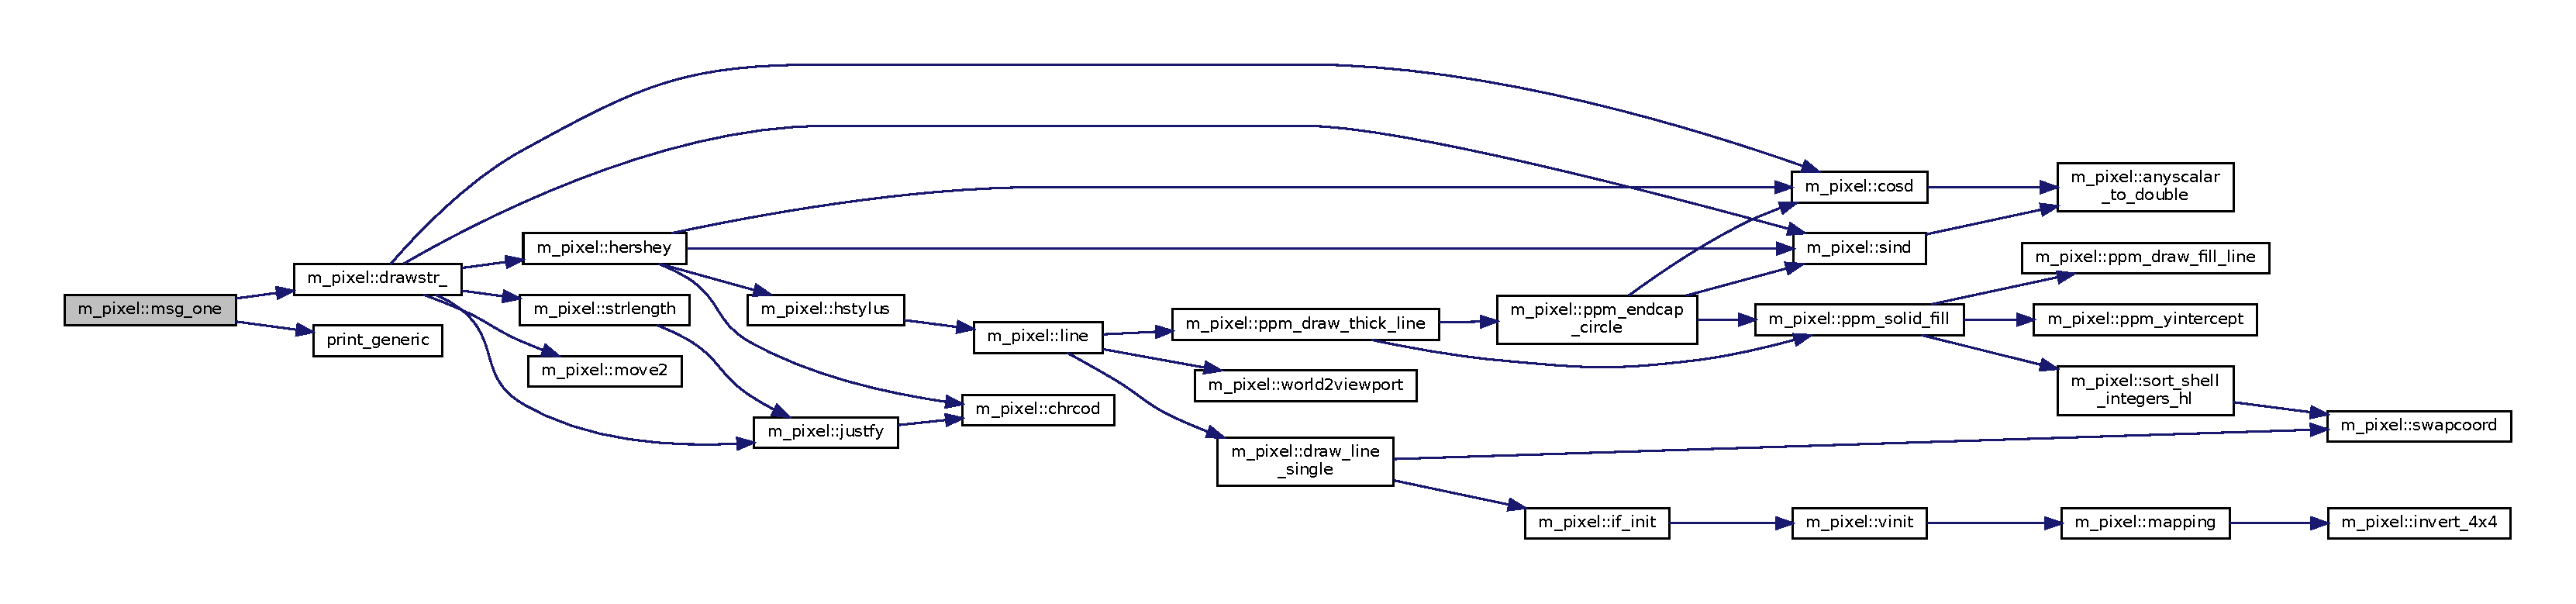
\includegraphics[width=350pt]{namespacem__pixel_a8c097c521deafffc765bd3f35eca423c_cgraph}
\end{center}
\end{figure}
\mbox{\Hypertarget{namespacem__pixel_af907f9c8cb0421cf9c5e6356e355382e}\label{namespacem__pixel_af907f9c8cb0421cf9c5e6356e355382e}} 
\index{m\+\_\+pixel@{m\+\_\+pixel}!msg\+\_\+scalar@{msg\+\_\+scalar}}
\index{msg\+\_\+scalar@{msg\+\_\+scalar}!m\+\_\+pixel@{m\+\_\+pixel}}
\subsubsection{\texorpdfstring{msg\+\_\+scalar()}{msg\_scalar()}}
{\footnotesize\ttfamily subroutine m\+\_\+pixel\+::msg\+\_\+scalar (\begin{DoxyParamCaption}\item[{class($\ast$), intent(in), optional}]{generic0,  }\item[{class($\ast$), intent(in), optional}]{generic1,  }\item[{class($\ast$), intent(in), optional}]{generic2,  }\item[{class($\ast$), intent(in), optional}]{generic3,  }\item[{class($\ast$), intent(in), optional}]{generic4,  }\item[{class($\ast$), intent(in), optional}]{generic5,  }\item[{class($\ast$), intent(in), optional}]{generic6,  }\item[{class($\ast$), intent(in), optional}]{generic7,  }\item[{class($\ast$), intent(in), optional}]{generic8,  }\item[{class($\ast$), intent(in), optional}]{generic9,  }\item[{class($\ast$), intent(in), optional}]{generica,  }\item[{class($\ast$), intent(in), optional}]{genericb,  }\item[{class($\ast$), intent(in), optional}]{genericc,  }\item[{class($\ast$), intent(in), optional}]{genericd,  }\item[{class($\ast$), intent(in), optional}]{generice,  }\item[{class($\ast$), intent(in), optional}]{genericf,  }\item[{class($\ast$), intent(in), optional}]{genericg,  }\item[{class($\ast$), intent(in), optional}]{generich,  }\item[{class($\ast$), intent(in), optional}]{generici,  }\item[{class($\ast$), intent(in), optional}]{genericj,  }\item[{logical, intent(in), optional}]{nospace }\end{DoxyParamCaption})\hspace{0.3cm}{\ttfamily [private]}}



\subsubsection*{N\+A\+ME}

drawstr(3f) -\/ \mbox{[}M\+\_\+msg\mbox{]} converts any standard scalar type to a string and prints it (L\+I\+C\+E\+N\+SE\+:PD) 

\subsubsection*{S\+Y\+N\+O\+P\+S\+IS}

\begin{DoxyVerb}subroutine drawstr(g0,g1,g2,g3,g4,g5,g6,g7,g8,g9,ga,gb,gc,gd,ge,gf,gg,gh,gi,gj,nospace)

 class(*),intent(in),optional  :: g0,g1,g2,g3,g4,g5,g6,g7,g8,g9
 class(*),intent(in),optional  :: ga,gb,gc,gd,ge,gf,gg,gh,gi,gj
 logical,intent(in),optional   :: nospace
\end{DoxyVerb}


\subsubsection*{D\+E\+S\+C\+R\+I\+P\+T\+I\+ON}

drawstr(3f) builds a space-\/separated string from up to twenty scalar values.

\subsubsection*{O\+P\+T\+I\+O\+NS}

g\mbox{[}0-\/9a-\/j\mbox{]} optional value to print the value of after the message. May be of type I\+N\+T\+E\+G\+ER, L\+O\+G\+I\+C\+AL, R\+E\+AL, D\+O\+U\+B\+L\+E\+P\+R\+E\+C\+I\+S\+I\+ON, C\+O\+M\+P\+L\+EX, or C\+H\+A\+R\+A\+C\+T\+ER.

Optionally, all the generic values can be single-\/dimensioned arrays. Currently, mixing scalar arguments and array arguments is not supported.

nospace if nospace=.true., then no spaces are added between values

\subsubsection*{E\+X\+A\+M\+P\+L\+ES}

Sample program\+:

program demo\+\_\+msg use M\+\_\+pixel, only \+: str implicit none character(len=\+:),allocatable \+:\+: pr character(len=\+:),allocatable \+:\+: frmt integer \+:\+: biggest

pr=str(\textquotesingle{}H\+U\+G\+E(3f) integers\textquotesingle{},huge(0),\textquotesingle{}and real\textquotesingle{},huge(0.\+0),\textquotesingle{}and double\textquotesingle{},huge(0.\+0d0)) write($\ast$,\textquotesingle{}(a)\textquotesingle{})pr pr=str(\textquotesingle{}real \+:\textquotesingle{},huge(0.\+0),0.\+0,12345.\+6789,tiny(0.\+0) ) write($\ast$,\textquotesingle{}(a)\textquotesingle{})pr pr=str(\textquotesingle{}doubleprecision \+:\textquotesingle{},huge(0.\+0d0),0.\+0d0,12345.\+6789d0,tiny(0.\+0d0) ) write($\ast$,\textquotesingle{}(a)\textquotesingle{})pr pr=str(\textquotesingle{}complex \+:\textquotesingle{},cmplx(huge(0.\+0),tiny(0.\+0)) ) write($\ast$,\textquotesingle{}(a)\textquotesingle{})pr

! create a format on the fly biggest=huge(0) frmt=str(\textquotesingle{}($\ast$(i\textquotesingle{},int(log10(real(biggest))),\textquotesingle{}\+:,1x))\textquotesingle{},nospace=.true.) write($\ast$,$\ast$)\textquotesingle{}format=\textquotesingle{},frmt

! although it will often work, using str(3f) in an I/O statement is not recommended ! because if an error occurs str(3f) will try to write while part of an I/O statement ! which not all compilers can handle and is currently non-\/standard write($\ast$,$\ast$)str(\textquotesingle{}program will now stop\textquotesingle{})

end program demo\+\_\+msg

Output

H\+U\+G\+E(3f) integers 2147483647 and real 3.\+40282347E+38 and double 1.\+7976931348623157E+308 real \+: 3.\+40282347E+38 0.\+00000000 12345.\+6787 1.\+17549435E-\/38 doubleprecision \+: 1.\+7976931348623157E+308 0.\+0000000000000000 12345.\+678900000001 2.\+2250738585072014E-\/308 complex \+: (3.\+40282347E+38,1.\+17549435E-\/38) format=($\ast$(i9\+:,1x)) program will now stop

\subsubsection*{A\+U\+T\+H\+OR}

John S. Urban

\subsubsection*{L\+I\+C\+E\+N\+SE}

Public Domain 

References drawstr\+\_\+(), and print\+\_\+generic().

Here is the call graph for this function\+:
\nopagebreak
\begin{figure}[H]
\begin{center}
\leavevmode
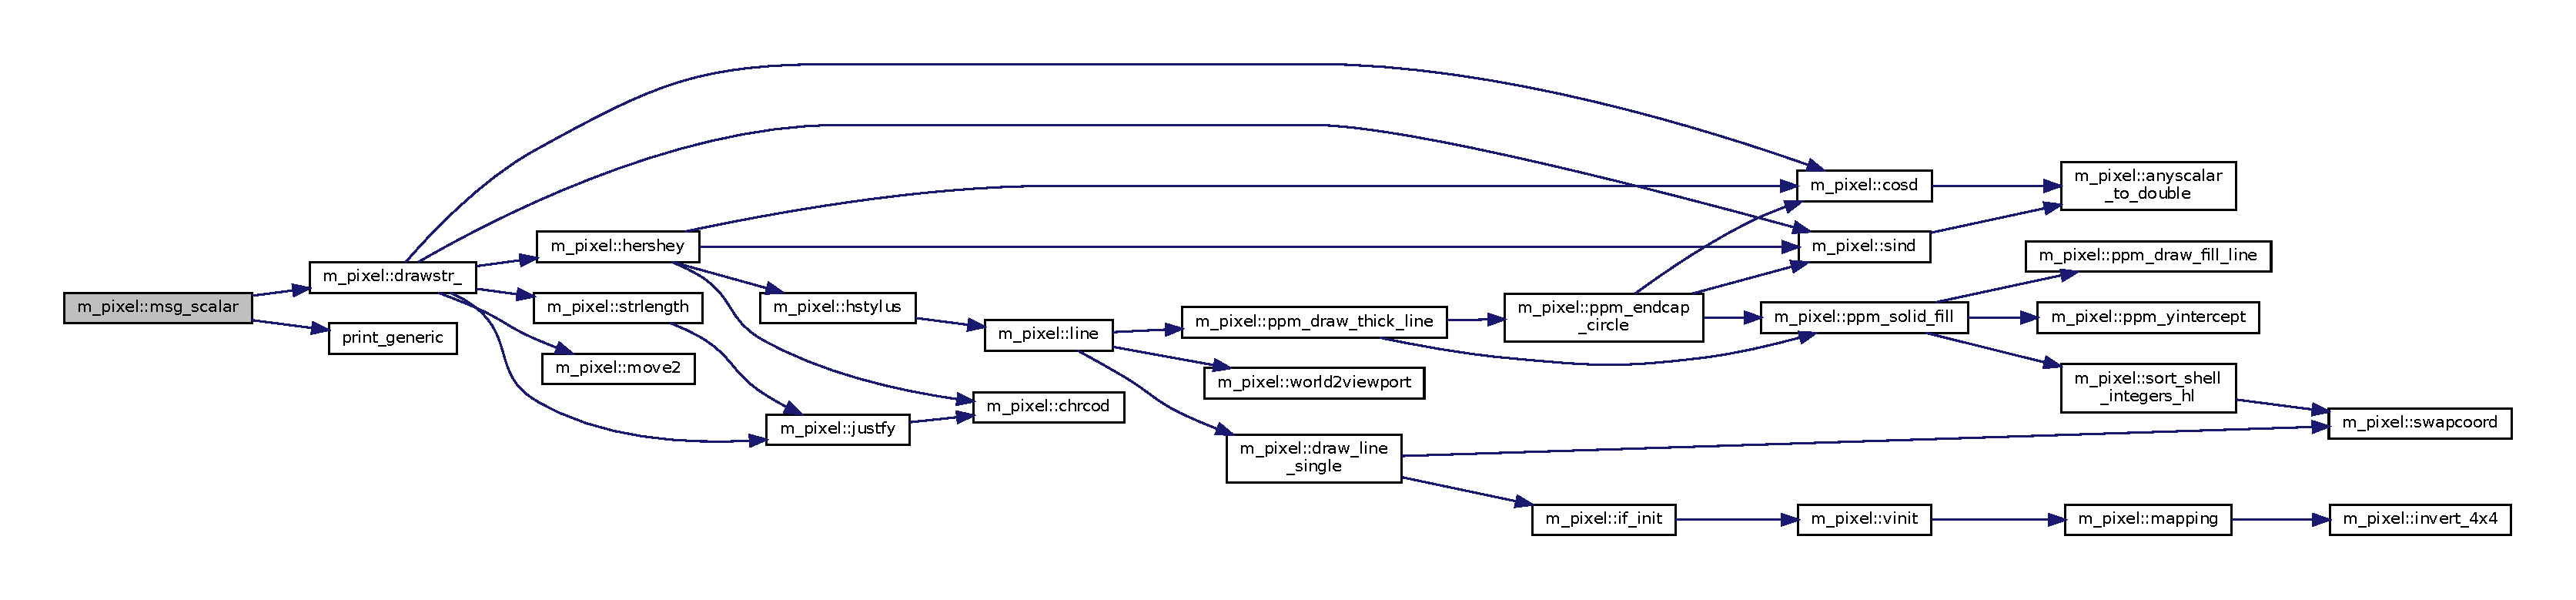
\includegraphics[width=350pt]{namespacem__pixel_af907f9c8cb0421cf9c5e6356e355382e_cgraph}
\end{center}
\end{figure}
\mbox{\Hypertarget{namespacem__pixel_a80dece6adac704024a5a76efee697770}\label{namespacem__pixel_a80dece6adac704024a5a76efee697770}} 
\index{m\+\_\+pixel@{m\+\_\+pixel}!ortho2@{ortho2}}
\index{ortho2@{ortho2}!m\+\_\+pixel@{m\+\_\+pixel}}
\subsubsection{\texorpdfstring{ortho2()}{ortho2()}}
{\footnotesize\ttfamily subroutine, public m\+\_\+pixel\+::ortho2 (\begin{DoxyParamCaption}\item[{real, intent(in)}]{left,  }\item[{real, intent(in)}]{right,  }\item[{real, intent(in)}]{bottom,  }\item[{real, intent(in)}]{top }\end{DoxyParamCaption})}



References mapping(), p\+\_\+window\+\_\+bottom, p\+\_\+window\+\_\+left, p\+\_\+window\+\_\+right, and p\+\_\+window\+\_\+top.

Here is the call graph for this function\+:
\nopagebreak
\begin{figure}[H]
\begin{center}
\leavevmode
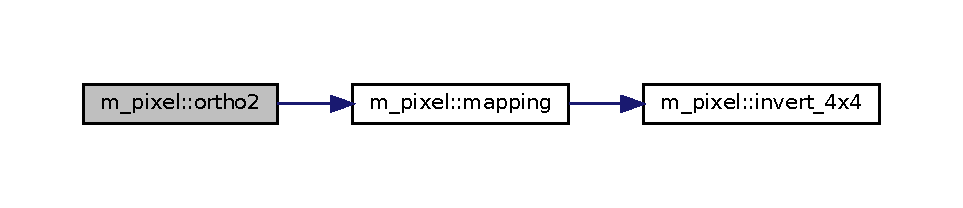
\includegraphics[width=350pt]{namespacem__pixel_a80dece6adac704024a5a76efee697770_cgraph}
\end{center}
\end{figure}
Here is the caller graph for this function\+:
\nopagebreak
\begin{figure}[H]
\begin{center}
\leavevmode
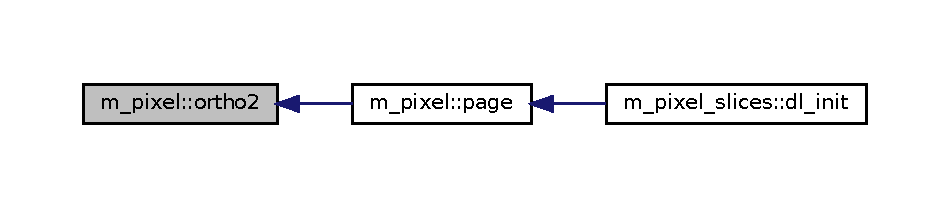
\includegraphics[width=350pt]{namespacem__pixel_a80dece6adac704024a5a76efee697770_icgraph}
\end{center}
\end{figure}
\mbox{\Hypertarget{namespacem__pixel_a6733a8657ca9f51b2648690dbae258c9}\label{namespacem__pixel_a6733a8657ca9f51b2648690dbae258c9}} 
\index{m\+\_\+pixel@{m\+\_\+pixel}!page@{page}}
\index{page@{page}!m\+\_\+pixel@{m\+\_\+pixel}}
\subsubsection{\texorpdfstring{page()}{page()}}
{\footnotesize\ttfamily subroutine, public m\+\_\+pixel\+::page (\begin{DoxyParamCaption}\item[{real, intent(in)}]{xsmall,  }\item[{real, intent(in)}]{xlarge,  }\item[{real, intent(in)}]{ysmall,  }\item[{real, intent(in)}]{ylarge }\end{DoxyParamCaption})}



References getdisplaysize(), journal(), ortho2(), p\+\_\+debug, and viewport().

Here is the call graph for this function\+:
\nopagebreak
\begin{figure}[H]
\begin{center}
\leavevmode
\includegraphics[width=350pt]{namespacem__pixel_a6733a8657ca9f51b2648690dbae258c9_cgraph}
\end{center}
\end{figure}
Here is the caller graph for this function\+:
\nopagebreak
\begin{figure}[H]
\begin{center}
\leavevmode
\includegraphics[width=327pt]{namespacem__pixel_a6733a8657ca9f51b2648690dbae258c9_icgraph}
\end{center}
\end{figure}
\mbox{\Hypertarget{namespacem__pixel_a11234e0b33104eb0afb24f928b072053}\label{namespacem__pixel_a11234e0b33104eb0afb24f928b072053}} 
\index{m\+\_\+pixel@{m\+\_\+pixel}!point2@{point2}}
\index{point2@{point2}!m\+\_\+pixel@{m\+\_\+pixel}}
\subsubsection{\texorpdfstring{point2()}{point2()}}
{\footnotesize\ttfamily subroutine, public m\+\_\+pixel\+::point2 (\begin{DoxyParamCaption}\item[{real, intent(in)}]{x,  }\item[{real, intent(in)}]{y }\end{DoxyParamCaption})}



References line().

Here is the call graph for this function\+:
\nopagebreak
\begin{figure}[H]
\begin{center}
\leavevmode
\includegraphics[width=350pt]{namespacem__pixel_a11234e0b33104eb0afb24f928b072053_cgraph}
\end{center}
\end{figure}
\mbox{\Hypertarget{namespacem__pixel_a5ee5c618d117b150b661e15517a3d408}\label{namespacem__pixel_a5ee5c618d117b150b661e15517a3d408}} 
\index{m\+\_\+pixel@{m\+\_\+pixel}!polar\+\_\+to\+\_\+cartesian@{polar\+\_\+to\+\_\+cartesian}}
\index{polar\+\_\+to\+\_\+cartesian@{polar\+\_\+to\+\_\+cartesian}!m\+\_\+pixel@{m\+\_\+pixel}}
\subsubsection{\texorpdfstring{polar\+\_\+to\+\_\+cartesian()}{polar\_to\_cartesian()}}
{\footnotesize\ttfamily subroutine, public m\+\_\+pixel\+::polar\+\_\+to\+\_\+cartesian (\begin{DoxyParamCaption}\item[{real, intent(in)}]{radius,  }\item[{real, intent(in)}]{inclination,  }\item[{real, intent(out)}]{x,  }\item[{real, intent(out)}]{y }\end{DoxyParamCaption})}

\mbox{\Hypertarget{namespacem__pixel_a996117d631dce0e92056a0c486be5109}\label{namespacem__pixel_a996117d631dce0e92056a0c486be5109}} 
\index{m\+\_\+pixel@{m\+\_\+pixel}!poly2@{poly2}}
\index{poly2@{poly2}!m\+\_\+pixel@{m\+\_\+pixel}}
\subsubsection{\texorpdfstring{poly2()}{poly2()}}
{\footnotesize\ttfamily subroutine, public m\+\_\+pixel\+::poly2 (\begin{DoxyParamCaption}\item[{integer, intent(in)}]{n,  }\item[{real, dimension(2, n), intent(in)}]{points }\end{DoxyParamCaption})}



References ppm\+\_\+solid\+\_\+fill(), and world2viewport().

Here is the call graph for this function\+:
\nopagebreak
\begin{figure}[H]
\begin{center}
\leavevmode
\includegraphics[width=350pt]{namespacem__pixel_a996117d631dce0e92056a0c486be5109_cgraph}
\end{center}
\end{figure}
Here is the caller graph for this function\+:
\nopagebreak
\begin{figure}[H]
\begin{center}
\leavevmode
\includegraphics[width=313pt]{namespacem__pixel_a996117d631dce0e92056a0c486be5109_icgraph}
\end{center}
\end{figure}
\mbox{\Hypertarget{namespacem__pixel_a0678be124889fb633475a6724ddb6640}\label{namespacem__pixel_a0678be124889fb633475a6724ddb6640}} 
\index{m\+\_\+pixel@{m\+\_\+pixel}!polyline2@{polyline2}}
\index{polyline2@{polyline2}!m\+\_\+pixel@{m\+\_\+pixel}}
\subsubsection{\texorpdfstring{polyline2()}{polyline2()}}
{\footnotesize\ttfamily subroutine, public m\+\_\+pixel\+::polyline2 (\begin{DoxyParamCaption}\item[{class($\ast$), dimension(\+:), intent(in)}]{x,  }\item[{class($\ast$), dimension(\+:), intent(in), optional}]{y }\end{DoxyParamCaption})}



References anyscalar\+\_\+to\+\_\+real(), draw2(), and move2().

Here is the call graph for this function\+:
\nopagebreak
\begin{figure}[H]
\begin{center}
\leavevmode
\includegraphics[width=350pt]{namespacem__pixel_a0678be124889fb633475a6724ddb6640_cgraph}
\end{center}
\end{figure}
\mbox{\Hypertarget{namespacem__pixel_a6f75bc951acd07267e0841ca5985d8b7}\label{namespacem__pixel_a6f75bc951acd07267e0841ca5985d8b7}} 
\index{m\+\_\+pixel@{m\+\_\+pixel}!ppm\+\_\+draw\+\_\+fill\+\_\+line@{ppm\+\_\+draw\+\_\+fill\+\_\+line}}
\index{ppm\+\_\+draw\+\_\+fill\+\_\+line@{ppm\+\_\+draw\+\_\+fill\+\_\+line}!m\+\_\+pixel@{m\+\_\+pixel}}
\subsubsection{\texorpdfstring{ppm\+\_\+draw\+\_\+fill\+\_\+line()}{ppm\_draw\_fill\_line()}}
{\footnotesize\ttfamily subroutine m\+\_\+pixel\+::ppm\+\_\+draw\+\_\+fill\+\_\+line (\begin{DoxyParamCaption}\item[{integer, intent(in)}]{xstart,  }\item[{integer, intent(in)}]{ystart,  }\item[{integer, intent(in)}]{x,  }\item[{integer, intent(in)}]{y }\end{DoxyParamCaption})\hspace{0.3cm}{\ttfamily [private]}}



References p\+\_\+color\+\_\+index, and p\+\_\+pixel.

Here is the caller graph for this function\+:
\nopagebreak
\begin{figure}[H]
\begin{center}
\leavevmode
\includegraphics[width=350pt]{namespacem__pixel_a6f75bc951acd07267e0841ca5985d8b7_icgraph}
\end{center}
\end{figure}
\mbox{\Hypertarget{namespacem__pixel_a1629b7134d0ea4b0f301ca23df764b8e}\label{namespacem__pixel_a1629b7134d0ea4b0f301ca23df764b8e}} 
\index{m\+\_\+pixel@{m\+\_\+pixel}!ppm\+\_\+draw\+\_\+thick\+\_\+line@{ppm\+\_\+draw\+\_\+thick\+\_\+line}}
\index{ppm\+\_\+draw\+\_\+thick\+\_\+line@{ppm\+\_\+draw\+\_\+thick\+\_\+line}!m\+\_\+pixel@{m\+\_\+pixel}}
\subsubsection{\texorpdfstring{ppm\+\_\+draw\+\_\+thick\+\_\+line()}{ppm\_draw\_thick\_line()}}
{\footnotesize\ttfamily subroutine m\+\_\+pixel\+::ppm\+\_\+draw\+\_\+thick\+\_\+line (\begin{DoxyParamCaption}\item[{integer, intent(in)}]{inx1,  }\item[{integer, intent(in)}]{iny1,  }\item[{integer, intent(in)}]{inx2,  }\item[{integer, intent(in)}]{iny2 }\end{DoxyParamCaption})\hspace{0.3cm}{\ttfamily [private]}}



References p\+\_\+width, ppm\+\_\+endcap\+\_\+circle(), and ppm\+\_\+solid\+\_\+fill().

Here is the call graph for this function\+:
\nopagebreak
\begin{figure}[H]
\begin{center}
\leavevmode
\includegraphics[width=350pt]{namespacem__pixel_a1629b7134d0ea4b0f301ca23df764b8e_cgraph}
\end{center}
\end{figure}
Here is the caller graph for this function\+:
\nopagebreak
\begin{figure}[H]
\begin{center}
\leavevmode
\includegraphics[width=350pt]{namespacem__pixel_a1629b7134d0ea4b0f301ca23df764b8e_icgraph}
\end{center}
\end{figure}
\mbox{\Hypertarget{namespacem__pixel_aede24c612504a3e416840e6242c2d8fb}\label{namespacem__pixel_aede24c612504a3e416840e6242c2d8fb}} 
\index{m\+\_\+pixel@{m\+\_\+pixel}!ppm\+\_\+endcap\+\_\+circle@{ppm\+\_\+endcap\+\_\+circle}}
\index{ppm\+\_\+endcap\+\_\+circle@{ppm\+\_\+endcap\+\_\+circle}!m\+\_\+pixel@{m\+\_\+pixel}}
\subsubsection{\texorpdfstring{ppm\+\_\+endcap\+\_\+circle()}{ppm\_endcap\_circle()}}
{\footnotesize\ttfamily subroutine m\+\_\+pixel\+::ppm\+\_\+endcap\+\_\+circle (\begin{DoxyParamCaption}\item[{integer, intent(in)}]{x,  }\item[{integer, intent(in)}]{y }\end{DoxyParamCaption})\hspace{0.3cm}{\ttfamily [private]}}



References cosd(), p\+\_\+width, ppm\+\_\+solid\+\_\+fill(), and sind().

Here is the call graph for this function\+:
\nopagebreak
\begin{figure}[H]
\begin{center}
\leavevmode
\includegraphics[width=350pt]{namespacem__pixel_aede24c612504a3e416840e6242c2d8fb_cgraph}
\end{center}
\end{figure}
Here is the caller graph for this function\+:
\nopagebreak
\begin{figure}[H]
\begin{center}
\leavevmode
\includegraphics[width=350pt]{namespacem__pixel_aede24c612504a3e416840e6242c2d8fb_icgraph}
\end{center}
\end{figure}
\mbox{\Hypertarget{namespacem__pixel_aedaf33a27e9899da22c2497aff2af903}\label{namespacem__pixel_aedaf33a27e9899da22c2497aff2af903}} 
\index{m\+\_\+pixel@{m\+\_\+pixel}!ppm\+\_\+solid\+\_\+fill@{ppm\+\_\+solid\+\_\+fill}}
\index{ppm\+\_\+solid\+\_\+fill@{ppm\+\_\+solid\+\_\+fill}!m\+\_\+pixel@{m\+\_\+pixel}}
\subsubsection{\texorpdfstring{ppm\+\_\+solid\+\_\+fill()}{ppm\_solid\_fill()}}
{\footnotesize\ttfamily subroutine m\+\_\+pixel\+::ppm\+\_\+solid\+\_\+fill (\begin{DoxyParamCaption}\item[{integer, dimension(0\+:n-\/1), intent(in)}]{x,  }\item[{integer, dimension(0\+:n-\/1), intent(in)}]{y,  }\item[{integer, intent(in)}]{n }\end{DoxyParamCaption})\hspace{0.3cm}{\ttfamily [private]}}



References p\+\_\+debug, p\+\_\+viewport\+\_\+height, p\+\_\+viewport\+\_\+width, ppm\+\_\+draw\+\_\+fill\+\_\+line(), ppm\+\_\+yintercept(), and sort\+\_\+shell\+\_\+integers\+\_\+hl().

Here is the call graph for this function\+:
\nopagebreak
\begin{figure}[H]
\begin{center}
\leavevmode
\includegraphics[width=350pt]{namespacem__pixel_aedaf33a27e9899da22c2497aff2af903_cgraph}
\end{center}
\end{figure}
Here is the caller graph for this function\+:
\nopagebreak
\begin{figure}[H]
\begin{center}
\leavevmode
\includegraphics[width=350pt]{namespacem__pixel_aedaf33a27e9899da22c2497aff2af903_icgraph}
\end{center}
\end{figure}
\mbox{\Hypertarget{namespacem__pixel_a4924b3a5033acb74a4f4df60a4ba21eb}\label{namespacem__pixel_a4924b3a5033acb74a4f4df60a4ba21eb}} 
\index{m\+\_\+pixel@{m\+\_\+pixel}!ppm\+\_\+yintercept@{ppm\+\_\+yintercept}}
\index{ppm\+\_\+yintercept@{ppm\+\_\+yintercept}!m\+\_\+pixel@{m\+\_\+pixel}}
\subsubsection{\texorpdfstring{ppm\+\_\+yintercept()}{ppm\_yintercept()}}
{\footnotesize\ttfamily logical function m\+\_\+pixel\+::ppm\+\_\+yintercept (\begin{DoxyParamCaption}\item[{integer}]{yscan,  }\item[{integer}]{x1,  }\item[{integer}]{y1,  }\item[{integer}]{x2,  }\item[{integer}]{y2,  }\item[{integer}]{xintercept,  }\item[{integer}]{yprev }\end{DoxyParamCaption})\hspace{0.3cm}{\ttfamily [private]}}

Here is the caller graph for this function\+:
\nopagebreak
\begin{figure}[H]
\begin{center}
\leavevmode
\includegraphics[width=350pt]{namespacem__pixel_a4924b3a5033acb74a4f4df60a4ba21eb_icgraph}
\end{center}
\end{figure}
\mbox{\Hypertarget{namespacem__pixel_acc868686f05b7e0b3cd33bf9d1c6bb98}\label{namespacem__pixel_acc868686f05b7e0b3cd33bf9d1c6bb98}} 
\index{m\+\_\+pixel@{m\+\_\+pixel}!prefsize@{prefsize}}
\index{prefsize@{prefsize}!m\+\_\+pixel@{m\+\_\+pixel}}
\subsubsection{\texorpdfstring{prefsize()}{prefsize()}}
{\footnotesize\ttfamily subroutine, public m\+\_\+pixel\+::prefsize (\begin{DoxyParamCaption}\item[{integer, intent(in)}]{x,  }\item[{integer, intent(in)}]{y }\end{DoxyParamCaption})}



References p\+\_\+viewport\+\_\+height, and p\+\_\+viewport\+\_\+width.

\mbox{\Hypertarget{namespacem__pixel_ab2bb47aea567667b1b92c8265bcb36fb}\label{namespacem__pixel_ab2bb47aea567667b1b92c8265bcb36fb}} 
\index{m\+\_\+pixel@{m\+\_\+pixel}!print\+\_\+ascii@{print\+\_\+ascii}}
\index{print\+\_\+ascii@{print\+\_\+ascii}!m\+\_\+pixel@{m\+\_\+pixel}}
\subsubsection{\texorpdfstring{print\+\_\+ascii()}{print\_ascii()}}
{\footnotesize\ttfamily subroutine, public m\+\_\+pixel\+::print\+\_\+ascii (\begin{DoxyParamCaption}\item[{character(len=$\ast$), intent(in), optional}]{filename }\end{DoxyParamCaption})}



References if\+\_\+init(), and p\+\_\+pixel.

Here is the call graph for this function\+:
\nopagebreak
\begin{figure}[H]
\begin{center}
\leavevmode
\includegraphics[width=350pt]{namespacem__pixel_ab2bb47aea567667b1b92c8265bcb36fb_cgraph}
\end{center}
\end{figure}
\mbox{\Hypertarget{namespacem__pixel_a01797b04ce7c693c3fd6a841e8d1de48}\label{namespacem__pixel_a01797b04ce7c693c3fd6a841e8d1de48}} 
\index{m\+\_\+pixel@{m\+\_\+pixel}!print\+\_\+ppm@{print\+\_\+ppm}}
\index{print\+\_\+ppm@{print\+\_\+ppm}!m\+\_\+pixel@{m\+\_\+pixel}}
\subsubsection{\texorpdfstring{print\+\_\+ppm()}{print\_ppm()}}
{\footnotesize\ttfamily subroutine, public m\+\_\+pixel\+::print\+\_\+ppm (\begin{DoxyParamCaption}\item[{character(len=$\ast$), intent(in)}]{filename }\end{DoxyParamCaption})}



References if\+\_\+init(), j, p\+\_\+colormap, and p\+\_\+pixel.

Here is the call graph for this function\+:
\nopagebreak
\begin{figure}[H]
\begin{center}
\leavevmode
\includegraphics[width=350pt]{namespacem__pixel_a01797b04ce7c693c3fd6a841e8d1de48_cgraph}
\end{center}
\end{figure}
\mbox{\Hypertarget{namespacem__pixel_a664375b036092dbebe1bccdc67254e1d}\label{namespacem__pixel_a664375b036092dbebe1bccdc67254e1d}} 
\index{m\+\_\+pixel@{m\+\_\+pixel}!rdraw2@{rdraw2}}
\index{rdraw2@{rdraw2}!m\+\_\+pixel@{m\+\_\+pixel}}
\subsubsection{\texorpdfstring{rdraw2()}{rdraw2()}}
{\footnotesize\ttfamily subroutine, public m\+\_\+pixel\+::rdraw2 (\begin{DoxyParamCaption}\item[{real, intent(in)}]{xdelta,  }\item[{real, intent(in)}]{ydelta }\end{DoxyParamCaption})}



References line(), p\+\_\+x, and p\+\_\+y.

Here is the call graph for this function\+:
\nopagebreak
\begin{figure}[H]
\begin{center}
\leavevmode
\includegraphics[width=350pt]{namespacem__pixel_a664375b036092dbebe1bccdc67254e1d_cgraph}
\end{center}
\end{figure}
\mbox{\Hypertarget{namespacem__pixel_a5435aa0d9d6048a62c09d7d90665b958}\label{namespacem__pixel_a5435aa0d9d6048a62c09d7d90665b958}} 
\index{m\+\_\+pixel@{m\+\_\+pixel}!rect@{rect}}
\index{rect@{rect}!m\+\_\+pixel@{m\+\_\+pixel}}
\subsubsection{\texorpdfstring{rect()}{rect()}}
{\footnotesize\ttfamily subroutine, public m\+\_\+pixel\+::rect (\begin{DoxyParamCaption}\item[{real, intent(in)}]{x1,  }\item[{real, intent(in)}]{y1,  }\item[{real, intent(in)}]{x2,  }\item[{real, intent(in)}]{y2 }\end{DoxyParamCaption})}



References draw2(), and move2().

Here is the call graph for this function\+:
\nopagebreak
\begin{figure}[H]
\begin{center}
\leavevmode
\includegraphics[width=350pt]{namespacem__pixel_a5435aa0d9d6048a62c09d7d90665b958_cgraph}
\end{center}
\end{figure}
\mbox{\Hypertarget{namespacem__pixel_a4dd5383ae0616511d16c996903a971dc}\label{namespacem__pixel_a4dd5383ae0616511d16c996903a971dc}} 
\index{m\+\_\+pixel@{m\+\_\+pixel}!rgbcmy@{rgbcmy}}
\index{rgbcmy@{rgbcmy}!m\+\_\+pixel@{m\+\_\+pixel}}
\subsubsection{\texorpdfstring{rgbcmy()}{rgbcmy()}}
{\footnotesize\ttfamily subroutine, private m\+\_\+pixel\+::rgbcmy (\begin{DoxyParamCaption}\item[{real, intent(in)}]{r,  }\item[{real, intent(in)}]{g,  }\item[{real, intent(in)}]{b,  }\item[{real, intent(out)}]{c,  }\item[{real, intent(out)}]{m,  }\item[{real, intent(out)}]{y,  }\item[{integer}]{status }\end{DoxyParamCaption})\hspace{0.3cm}{\ttfamily [private]}}

Here is the caller graph for this function\+:
\nopagebreak
\begin{figure}[H]
\begin{center}
\leavevmode
\includegraphics[width=350pt]{namespacem__pixel_a4dd5383ae0616511d16c996903a971dc_icgraph}
\end{center}
\end{figure}
\mbox{\Hypertarget{namespacem__pixel_a02bb73b68aeae5056ccf76868146b1b4}\label{namespacem__pixel_a02bb73b68aeae5056ccf76868146b1b4}} 
\index{m\+\_\+pixel@{m\+\_\+pixel}!rgbhls@{rgbhls}}
\index{rgbhls@{rgbhls}!m\+\_\+pixel@{m\+\_\+pixel}}
\subsubsection{\texorpdfstring{rgbhls()}{rgbhls()}}
{\footnotesize\ttfamily subroutine, private m\+\_\+pixel\+::rgbhls (\begin{DoxyParamCaption}\item[{real}]{r0,  }\item[{real}]{g0,  }\item[{real}]{b0,  }\item[{real}]{h,  }\item[{real}]{l,  }\item[{real}]{s,  }\item[{integer}]{status }\end{DoxyParamCaption})\hspace{0.3cm}{\ttfamily [private]}}

Here is the caller graph for this function\+:
\nopagebreak
\begin{figure}[H]
\begin{center}
\leavevmode
\includegraphics[width=350pt]{namespacem__pixel_a02bb73b68aeae5056ccf76868146b1b4_icgraph}
\end{center}
\end{figure}
\mbox{\Hypertarget{namespacem__pixel_a07ffb197bdcd075f5375e95b43c18915}\label{namespacem__pixel_a07ffb197bdcd075f5375e95b43c18915}} 
\index{m\+\_\+pixel@{m\+\_\+pixel}!rgbhvs@{rgbhvs}}
\index{rgbhvs@{rgbhvs}!m\+\_\+pixel@{m\+\_\+pixel}}
\subsubsection{\texorpdfstring{rgbhvs()}{rgbhvs()}}
{\footnotesize\ttfamily subroutine, private m\+\_\+pixel\+::rgbhvs (\begin{DoxyParamCaption}\item[{real, intent(in)}]{r0,  }\item[{real, intent(in)}]{g0,  }\item[{real, intent(in)}]{b0,  }\item[{real, intent(out)}]{h,  }\item[{real, intent(out)}]{v,  }\item[{real, intent(out)}]{s,  }\item[{integer}]{status }\end{DoxyParamCaption})\hspace{0.3cm}{\ttfamily [private]}}

Here is the caller graph for this function\+:
\nopagebreak
\begin{figure}[H]
\begin{center}
\leavevmode
\includegraphics[width=350pt]{namespacem__pixel_a07ffb197bdcd075f5375e95b43c18915_icgraph}
\end{center}
\end{figure}
\mbox{\Hypertarget{namespacem__pixel_a63a581cda811571c9ded805516f9d709}\label{namespacem__pixel_a63a581cda811571c9ded805516f9d709}} 
\index{m\+\_\+pixel@{m\+\_\+pixel}!rgbmono@{rgbmono}}
\index{rgbmono@{rgbmono}!m\+\_\+pixel@{m\+\_\+pixel}}
\subsubsection{\texorpdfstring{rgbmono()}{rgbmono()}}
{\footnotesize\ttfamily subroutine, public m\+\_\+pixel\+::rgbmono (\begin{DoxyParamCaption}\item[{real, intent(in)}]{rr,  }\item[{real, intent(in)}]{rg,  }\item[{real, intent(in)}]{rb,  }\item[{real, intent(out)}]{ri,  }\item[{integer, intent(out)}]{status }\end{DoxyParamCaption})}

\mbox{\Hypertarget{namespacem__pixel_a9f8175d7b5b349cd5c30a99100eef5c5}\label{namespacem__pixel_a9f8175d7b5b349cd5c30a99100eef5c5}} 
\index{m\+\_\+pixel@{m\+\_\+pixel}!rgbval@{rgbval}}
\index{rgbval@{rgbval}!m\+\_\+pixel@{m\+\_\+pixel}}
\subsubsection{\texorpdfstring{rgbval()}{rgbval()}}
{\footnotesize\ttfamily real function, private m\+\_\+pixel\+::rgbval (\begin{DoxyParamCaption}\item[{real}]{clr1,  }\item[{real}]{clr2,  }\item[{real}]{h }\end{DoxyParamCaption})\hspace{0.3cm}{\ttfamily [private]}}

Here is the caller graph for this function\+:
\nopagebreak
\begin{figure}[H]
\begin{center}
\leavevmode
\includegraphics[width=350pt]{namespacem__pixel_a9f8175d7b5b349cd5c30a99100eef5c5_icgraph}
\end{center}
\end{figure}
\mbox{\Hypertarget{namespacem__pixel_a0c025b24458dba5fb448f62cb10c7088}\label{namespacem__pixel_a0c025b24458dba5fb448f62cb10c7088}} 
\index{m\+\_\+pixel@{m\+\_\+pixel}!rgbyiq@{rgbyiq}}
\index{rgbyiq@{rgbyiq}!m\+\_\+pixel@{m\+\_\+pixel}}
\subsubsection{\texorpdfstring{rgbyiq()}{rgbyiq()}}
{\footnotesize\ttfamily subroutine, private m\+\_\+pixel\+::rgbyiq (\begin{DoxyParamCaption}\item[{real, intent(in)}]{r,  }\item[{real, intent(in)}]{g,  }\item[{real, intent(in)}]{b,  }\item[{real, intent(out)}]{y,  }\item[{real, intent(out)}]{i,  }\item[{real, intent(out)}]{q,  }\item[{integer}]{status }\end{DoxyParamCaption})\hspace{0.3cm}{\ttfamily [private]}}

Here is the caller graph for this function\+:
\nopagebreak
\begin{figure}[H]
\begin{center}
\leavevmode
\includegraphics[width=350pt]{namespacem__pixel_a0c025b24458dba5fb448f62cb10c7088_icgraph}
\end{center}
\end{figure}
\mbox{\Hypertarget{namespacem__pixel_a9b0fb9ccafe605fd6daf50c74347ed3a}\label{namespacem__pixel_a9b0fb9ccafe605fd6daf50c74347ed3a}} 
\index{m\+\_\+pixel@{m\+\_\+pixel}!rmove2@{rmove2}}
\index{rmove2@{rmove2}!m\+\_\+pixel@{m\+\_\+pixel}}
\subsubsection{\texorpdfstring{rmove2()}{rmove2()}}
{\footnotesize\ttfamily subroutine, public m\+\_\+pixel\+::rmove2 (\begin{DoxyParamCaption}\item[{real, intent(in)}]{Xdelta,  }\item[{real, intent(in)}]{Ydelta }\end{DoxyParamCaption})}



References p\+\_\+x, and p\+\_\+y.

\mbox{\Hypertarget{namespacem__pixel_a3ef23ce0230c47b30cb627ebd439daae}\label{namespacem__pixel_a3ef23ce0230c47b30cb627ebd439daae}} 
\index{m\+\_\+pixel@{m\+\_\+pixel}!sind@{sind}}
\index{sind@{sind}!m\+\_\+pixel@{m\+\_\+pixel}}
\subsubsection{\texorpdfstring{sind()}{sind()}}
{\footnotesize\ttfamily elemental real function, public m\+\_\+pixel\+::sind (\begin{DoxyParamCaption}\item[{class($\ast$), intent(in)}]{angle\+\_\+in\+\_\+degrees }\end{DoxyParamCaption})}



References anyscalar\+\_\+to\+\_\+double(), and degrees\+\_\+to\+\_\+radians.

Here is the call graph for this function\+:
\nopagebreak
\begin{figure}[H]
\begin{center}
\leavevmode
\includegraphics[width=307pt]{namespacem__pixel_a3ef23ce0230c47b30cb627ebd439daae_cgraph}
\end{center}
\end{figure}
Here is the caller graph for this function\+:
\nopagebreak
\begin{figure}[H]
\begin{center}
\leavevmode
\includegraphics[width=350pt]{namespacem__pixel_a3ef23ce0230c47b30cb627ebd439daae_icgraph}
\end{center}
\end{figure}
\mbox{\Hypertarget{namespacem__pixel_a4396c3ff36a080fbbfa859348203d0c7}\label{namespacem__pixel_a4396c3ff36a080fbbfa859348203d0c7}} 
\index{m\+\_\+pixel@{m\+\_\+pixel}!sort\+\_\+shell\+\_\+integers\+\_\+hl@{sort\+\_\+shell\+\_\+integers\+\_\+hl}}
\index{sort\+\_\+shell\+\_\+integers\+\_\+hl@{sort\+\_\+shell\+\_\+integers\+\_\+hl}!m\+\_\+pixel@{m\+\_\+pixel}}
\subsubsection{\texorpdfstring{sort\+\_\+shell\+\_\+integers\+\_\+hl()}{sort\_shell\_integers\_hl()}}
{\footnotesize\ttfamily subroutine m\+\_\+pixel\+::sort\+\_\+shell\+\_\+integers\+\_\+hl (\begin{DoxyParamCaption}\item[{integer, dimension(\+:), intent(inout)}]{iarray }\end{DoxyParamCaption})\hspace{0.3cm}{\ttfamily [private]}}



References swapcoord().

Here is the call graph for this function\+:
\nopagebreak
\begin{figure}[H]
\begin{center}
\leavevmode
\includegraphics[width=339pt]{namespacem__pixel_a4396c3ff36a080fbbfa859348203d0c7_cgraph}
\end{center}
\end{figure}
Here is the caller graph for this function\+:
\nopagebreak
\begin{figure}[H]
\begin{center}
\leavevmode
\includegraphics[width=350pt]{namespacem__pixel_a4396c3ff36a080fbbfa859348203d0c7_icgraph}
\end{center}
\end{figure}
\mbox{\Hypertarget{namespacem__pixel_aa24c465b23b0ddda341e97bc206fe249}\label{namespacem__pixel_aa24c465b23b0ddda341e97bc206fe249}} 
\index{m\+\_\+pixel@{m\+\_\+pixel}!state@{state}}
\index{state@{state}!m\+\_\+pixel@{m\+\_\+pixel}}
\subsubsection{\texorpdfstring{state()}{state()}}
{\footnotesize\ttfamily recursive subroutine, public m\+\_\+pixel\+::state (\begin{DoxyParamCaption}\item[{character(len=$\ast$), intent(in), optional}]{string }\end{DoxyParamCaption})}



References p\+\_\+color\+\_\+index, p\+\_\+colormap, p\+\_\+font, p\+\_\+nsegs, p\+\_\+text\+\_\+angle, p\+\_\+text\+\_\+height, p\+\_\+text\+\_\+width, p\+\_\+viewport\+\_\+bottom, p\+\_\+viewport\+\_\+height, p\+\_\+viewport\+\_\+left, p\+\_\+viewport\+\_\+right, p\+\_\+viewport\+\_\+top, p\+\_\+viewport\+\_\+width, p\+\_\+vinit\+\_\+called, p\+\_\+width, p\+\_\+window\+\_\+bottom, p\+\_\+window\+\_\+left, p\+\_\+window\+\_\+right, p\+\_\+window\+\_\+top, p\+\_\+x, p\+\_\+x\+\_\+centertext, p\+\_\+y, and p\+\_\+y\+\_\+centertext.

\mbox{\Hypertarget{namespacem__pixel_a0468f8d9308bade7f8f2a68a133271d2}\label{namespacem__pixel_a0468f8d9308bade7f8f2a68a133271d2}} 
\index{m\+\_\+pixel@{m\+\_\+pixel}!strlength@{strlength}}
\index{strlength@{strlength}!m\+\_\+pixel@{m\+\_\+pixel}}
\subsubsection{\texorpdfstring{strlength()}{strlength()}}
{\footnotesize\ttfamily real function, public m\+\_\+pixel\+::strlength (\begin{DoxyParamCaption}\item[{character(len=$\ast$), intent(in)}]{string }\end{DoxyParamCaption})}



References justfy(), and p\+\_\+text\+\_\+height.

Here is the call graph for this function\+:
\nopagebreak
\begin{figure}[H]
\begin{center}
\leavevmode
\includegraphics[width=350pt]{namespacem__pixel_a0468f8d9308bade7f8f2a68a133271d2_cgraph}
\end{center}
\end{figure}
Here is the caller graph for this function\+:
\nopagebreak
\begin{figure}[H]
\begin{center}
\leavevmode
\includegraphics[width=350pt]{namespacem__pixel_a0468f8d9308bade7f8f2a68a133271d2_icgraph}
\end{center}
\end{figure}
\mbox{\Hypertarget{namespacem__pixel_a063f74c3dd2f7f086dc47ec68abc22c9}\label{namespacem__pixel_a063f74c3dd2f7f086dc47ec68abc22c9}} 
\index{m\+\_\+pixel@{m\+\_\+pixel}!swapcoord@{swapcoord}}
\index{swapcoord@{swapcoord}!m\+\_\+pixel@{m\+\_\+pixel}}
\subsubsection{\texorpdfstring{swapcoord()}{swapcoord()}}
{\footnotesize\ttfamily subroutine m\+\_\+pixel\+::swapcoord (\begin{DoxyParamCaption}\item[{integer, intent(inout)}]{p1,  }\item[{integer, intent(inout)}]{p2 }\end{DoxyParamCaption})\hspace{0.3cm}{\ttfamily [private]}}

Here is the caller graph for this function\+:
\nopagebreak
\begin{figure}[H]
\begin{center}
\leavevmode
\includegraphics[width=350pt]{namespacem__pixel_a063f74c3dd2f7f086dc47ec68abc22c9_icgraph}
\end{center}
\end{figure}
\mbox{\Hypertarget{namespacem__pixel_a5e213461e9894b99c9e8f278d5c4a858}\label{namespacem__pixel_a5e213461e9894b99c9e8f278d5c4a858}} 
\index{m\+\_\+pixel@{m\+\_\+pixel}!textang@{textang}}
\index{textang@{textang}!m\+\_\+pixel@{m\+\_\+pixel}}
\subsubsection{\texorpdfstring{textang()}{textang()}}
{\footnotesize\ttfamily subroutine, public m\+\_\+pixel\+::textang (\begin{DoxyParamCaption}\item[{real, intent(in)}]{ang }\end{DoxyParamCaption})}



References cosd(), p\+\_\+text\+\_\+angle, p\+\_\+text\+\_\+cosine, p\+\_\+text\+\_\+sine, and sind().

Here is the call graph for this function\+:
\nopagebreak
\begin{figure}[H]
\begin{center}
\leavevmode
\includegraphics[width=350pt]{namespacem__pixel_a5e213461e9894b99c9e8f278d5c4a858_cgraph}
\end{center}
\end{figure}
\mbox{\Hypertarget{namespacem__pixel_a070e9fff1f2cd0c89d40c5d3c72b7f2c}\label{namespacem__pixel_a070e9fff1f2cd0c89d40c5d3c72b7f2c}} 
\index{m\+\_\+pixel@{m\+\_\+pixel}!textsize@{textsize}}
\index{textsize@{textsize}!m\+\_\+pixel@{m\+\_\+pixel}}
\subsubsection{\texorpdfstring{textsize()}{textsize()}}
{\footnotesize\ttfamily subroutine, public m\+\_\+pixel\+::textsize (\begin{DoxyParamCaption}\item[{real, intent(in)}]{width,  }\item[{real, intent(in)}]{height }\end{DoxyParamCaption})}



References p\+\_\+text\+\_\+height, p\+\_\+text\+\_\+width, and width.

\mbox{\Hypertarget{namespacem__pixel_a19ad6b65752322b0029a62cc0ebec3e8}\label{namespacem__pixel_a19ad6b65752322b0029a62cc0ebec3e8}} 
\index{m\+\_\+pixel@{m\+\_\+pixel}!vexit@{vexit}}
\index{vexit@{vexit}!m\+\_\+pixel@{m\+\_\+pixel}}
\subsubsection{\texorpdfstring{vexit()}{vexit()}}
{\footnotesize\ttfamily subroutine, public m\+\_\+pixel\+::vexit (\begin{DoxyParamCaption}{ }\end{DoxyParamCaption})}



References p\+\_\+pixel, and p\+\_\+vinit\+\_\+called.

\mbox{\Hypertarget{namespacem__pixel_ae74cf11194379dbf13069a61b06589a2}\label{namespacem__pixel_ae74cf11194379dbf13069a61b06589a2}} 
\index{m\+\_\+pixel@{m\+\_\+pixel}!vflush@{vflush}}
\index{vflush@{vflush}!m\+\_\+pixel@{m\+\_\+pixel}}
\subsubsection{\texorpdfstring{vflush()}{vflush()}}
{\footnotesize\ttfamily subroutine, public m\+\_\+pixel\+::vflush (\begin{DoxyParamCaption}{ }\end{DoxyParamCaption})}

\mbox{\Hypertarget{namespacem__pixel_a43247343cd316e3aa075b44b5166e2e9}\label{namespacem__pixel_a43247343cd316e3aa075b44b5166e2e9}} 
\index{m\+\_\+pixel@{m\+\_\+pixel}!viewport@{viewport}}
\index{viewport@{viewport}!m\+\_\+pixel@{m\+\_\+pixel}}
\subsubsection{\texorpdfstring{viewport()}{viewport()}}
{\footnotesize\ttfamily subroutine, public m\+\_\+pixel\+::viewport (\begin{DoxyParamCaption}\item[{real, intent(in)}]{left,  }\item[{real, intent(in)}]{right,  }\item[{real, intent(in)}]{bottom,  }\item[{real, intent(in)}]{top }\end{DoxyParamCaption})}



References mapping(), p\+\_\+viewport\+\_\+bottom, p\+\_\+viewport\+\_\+left, p\+\_\+viewport\+\_\+right, and p\+\_\+viewport\+\_\+top.

Here is the call graph for this function\+:
\nopagebreak
\begin{figure}[H]
\begin{center}
\leavevmode
\includegraphics[width=350pt]{namespacem__pixel_a43247343cd316e3aa075b44b5166e2e9_cgraph}
\end{center}
\end{figure}
Here is the caller graph for this function\+:
\nopagebreak
\begin{figure}[H]
\begin{center}
\leavevmode
\includegraphics[width=350pt]{namespacem__pixel_a43247343cd316e3aa075b44b5166e2e9_icgraph}
\end{center}
\end{figure}
\mbox{\Hypertarget{namespacem__pixel_a9e23c9a3a5f3b1482986f067fbf8487f}\label{namespacem__pixel_a9e23c9a3a5f3b1482986f067fbf8487f}} 
\index{m\+\_\+pixel@{m\+\_\+pixel}!viewport2world@{viewport2world}}
\index{viewport2world@{viewport2world}!m\+\_\+pixel@{m\+\_\+pixel}}
\subsubsection{\texorpdfstring{viewport2world()}{viewport2world()}}
{\footnotesize\ttfamily subroutine m\+\_\+pixel\+::viewport2world (\begin{DoxyParamCaption}\item[{real, intent(in)}]{xv,  }\item[{real, intent(in)}]{yv,  }\item[{real, intent(out)}]{xw,  }\item[{real, intent(out)}]{yw }\end{DoxyParamCaption})\hspace{0.3cm}{\ttfamily [private]}}



References p\+\_\+a, p\+\_\+b, p\+\_\+c, and p\+\_\+d.

\mbox{\Hypertarget{namespacem__pixel_ac03ca8f23fdadb60599b6ea4dc87a6d9}\label{namespacem__pixel_ac03ca8f23fdadb60599b6ea4dc87a6d9}} 
\index{m\+\_\+pixel@{m\+\_\+pixel}!vinit@{vinit}}
\index{vinit@{vinit}!m\+\_\+pixel@{m\+\_\+pixel}}
\subsubsection{\texorpdfstring{vinit()}{vinit()}}
{\footnotesize\ttfamily subroutine, public m\+\_\+pixel\+::vinit (\begin{DoxyParamCaption}\item[{character(len=$\ast$), optional}]{string }\end{DoxyParamCaption})}



References mapping(), p\+\_\+color\+\_\+index, p\+\_\+font, p\+\_\+inpolygon, p\+\_\+nsegs, p\+\_\+pixel, p\+\_\+polyvertex, p\+\_\+text\+\_\+angle, p\+\_\+text\+\_\+cosine, p\+\_\+text\+\_\+height, p\+\_\+text\+\_\+sine, p\+\_\+text\+\_\+width, p\+\_\+viewport\+\_\+bottom, p\+\_\+viewport\+\_\+height, p\+\_\+viewport\+\_\+left, p\+\_\+viewport\+\_\+right, p\+\_\+viewport\+\_\+top, p\+\_\+viewport\+\_\+width, p\+\_\+vinit\+\_\+called, p\+\_\+width, p\+\_\+window\+\_\+bottom, p\+\_\+window\+\_\+left, p\+\_\+window\+\_\+right, p\+\_\+window\+\_\+top, p\+\_\+x, p\+\_\+x\+\_\+centertext, p\+\_\+y, and p\+\_\+y\+\_\+centertext.

Here is the call graph for this function\+:
\nopagebreak
\begin{figure}[H]
\begin{center}
\leavevmode
\includegraphics[width=350pt]{namespacem__pixel_ac03ca8f23fdadb60599b6ea4dc87a6d9_cgraph}
\end{center}
\end{figure}
Here is the caller graph for this function\+:
\nopagebreak
\begin{figure}[H]
\begin{center}
\leavevmode
\includegraphics[width=350pt]{namespacem__pixel_ac03ca8f23fdadb60599b6ea4dc87a6d9_icgraph}
\end{center}
\end{figure}
\mbox{\Hypertarget{namespacem__pixel_a9d4aea8ae2eb15317b83fa03a11371b2}\label{namespacem__pixel_a9d4aea8ae2eb15317b83fa03a11371b2}} 
\index{m\+\_\+pixel@{m\+\_\+pixel}!world2viewport@{world2viewport}}
\index{world2viewport@{world2viewport}!m\+\_\+pixel@{m\+\_\+pixel}}
\subsubsection{\texorpdfstring{world2viewport()}{world2viewport()}}
{\footnotesize\ttfamily subroutine m\+\_\+pixel\+::world2viewport (\begin{DoxyParamCaption}\item[{real, intent(in)}]{xw,  }\item[{real, intent(in)}]{yw,  }\item[{real, intent(out)}]{xv,  }\item[{real, intent(out)}]{yv }\end{DoxyParamCaption})\hspace{0.3cm}{\ttfamily [private]}}



References p\+\_\+a, p\+\_\+b, p\+\_\+c, and p\+\_\+d.

Here is the caller graph for this function\+:
\nopagebreak
\begin{figure}[H]
\begin{center}
\leavevmode
\includegraphics[width=350pt]{namespacem__pixel_a9d4aea8ae2eb15317b83fa03a11371b2_icgraph}
\end{center}
\end{figure}
\mbox{\Hypertarget{namespacem__pixel_a1e0c43d36b35eafea921f91c31d8a478}\label{namespacem__pixel_a1e0c43d36b35eafea921f91c31d8a478}} 
\index{m\+\_\+pixel@{m\+\_\+pixel}!xcentertext@{xcentertext}}
\index{xcentertext@{xcentertext}!m\+\_\+pixel@{m\+\_\+pixel}}
\subsubsection{\texorpdfstring{xcentertext()}{xcentertext()}}
{\footnotesize\ttfamily subroutine, public m\+\_\+pixel\+::xcentertext (\begin{DoxyParamCaption}{ }\end{DoxyParamCaption})}



References p\+\_\+x\+\_\+centertext, and p\+\_\+y\+\_\+centertext.

\mbox{\Hypertarget{namespacem__pixel_a2e32105b5e77abf38768fec6b11376a3}\label{namespacem__pixel_a2e32105b5e77abf38768fec6b11376a3}} 
\index{m\+\_\+pixel@{m\+\_\+pixel}!ycentertext@{ycentertext}}
\index{ycentertext@{ycentertext}!m\+\_\+pixel@{m\+\_\+pixel}}
\subsubsection{\texorpdfstring{ycentertext()}{ycentertext()}}
{\footnotesize\ttfamily subroutine, public m\+\_\+pixel\+::ycentertext (\begin{DoxyParamCaption}{ }\end{DoxyParamCaption})}



References p\+\_\+x\+\_\+centertext, and p\+\_\+y\+\_\+centertext.

\mbox{\Hypertarget{namespacem__pixel_a0f4f12a4a769b8827a79b44f333eca28}\label{namespacem__pixel_a0f4f12a4a769b8827a79b44f333eca28}} 
\index{m\+\_\+pixel@{m\+\_\+pixel}!yiqrgb@{yiqrgb}}
\index{yiqrgb@{yiqrgb}!m\+\_\+pixel@{m\+\_\+pixel}}
\subsubsection{\texorpdfstring{yiqrgb()}{yiqrgb()}}
{\footnotesize\ttfamily subroutine m\+\_\+pixel\+::yiqrgb (\begin{DoxyParamCaption}\item[{real, intent(in)}]{y,  }\item[{real, intent(in)}]{i,  }\item[{real, intent(in)}]{q,  }\item[{real, intent(out)}]{r,  }\item[{real, intent(out)}]{g,  }\item[{real, intent(out)}]{b,  }\item[{integer}]{status }\end{DoxyParamCaption})\hspace{0.3cm}{\ttfamily [private]}}

Here is the caller graph for this function\+:
\nopagebreak
\begin{figure}[H]
\begin{center}
\leavevmode
\includegraphics[width=350pt]{namespacem__pixel_a0f4f12a4a769b8827a79b44f333eca28_icgraph}
\end{center}
\end{figure}


\subsection{Variable Documentation}
\mbox{\Hypertarget{namespacem__pixel_a6f1238ade91dacb2d8c24ac393f2f8f4}\label{namespacem__pixel_a6f1238ade91dacb2d8c24ac393f2f8f4}} 
\index{m\+\_\+pixel@{m\+\_\+pixel}!d\+\_\+black@{d\+\_\+black}}
\index{d\+\_\+black@{d\+\_\+black}!m\+\_\+pixel@{m\+\_\+pixel}}
\subsubsection{\texorpdfstring{d\+\_\+black}{d\_black}}
{\footnotesize\ttfamily integer(kind=c\+\_\+int), parameter, public m\+\_\+pixel\+::d\+\_\+black = 0\+\_\+\+C\+\_\+\+I\+NT}

\mbox{\Hypertarget{namespacem__pixel_af2a1f35244e511380fe83cc31ceb31a8}\label{namespacem__pixel_af2a1f35244e511380fe83cc31ceb31a8}} 
\index{m\+\_\+pixel@{m\+\_\+pixel}!d\+\_\+blue@{d\+\_\+blue}}
\index{d\+\_\+blue@{d\+\_\+blue}!m\+\_\+pixel@{m\+\_\+pixel}}
\subsubsection{\texorpdfstring{d\+\_\+blue}{d\_blue}}
{\footnotesize\ttfamily integer(kind=c\+\_\+int), parameter, public m\+\_\+pixel\+::d\+\_\+blue = 4\+\_\+\+C\+\_\+\+I\+NT}

\mbox{\Hypertarget{namespacem__pixel_a19f01bd571c0cf1d8a1cbb3f7d43bfae}\label{namespacem__pixel_a19f01bd571c0cf1d8a1cbb3f7d43bfae}} 
\index{m\+\_\+pixel@{m\+\_\+pixel}!d\+\_\+bold@{d\+\_\+bold}}
\index{d\+\_\+bold@{d\+\_\+bold}!m\+\_\+pixel@{m\+\_\+pixel}}
\subsubsection{\texorpdfstring{d\+\_\+bold}{d\_bold}}
{\footnotesize\ttfamily integer(kind=c\+\_\+short), parameter, public m\+\_\+pixel\+::d\+\_\+bold = 1\+\_\+\+C\+\_\+\+S\+H\+O\+RT}

\mbox{\Hypertarget{namespacem__pixel_ae996d01c0e74fed7a7dc923f2fce3f0a}\label{namespacem__pixel_ae996d01c0e74fed7a7dc923f2fce3f0a}} 
\index{m\+\_\+pixel@{m\+\_\+pixel}!d\+\_\+bottom@{d\+\_\+bottom}}
\index{d\+\_\+bottom@{d\+\_\+bottom}!m\+\_\+pixel@{m\+\_\+pixel}}
\subsubsection{\texorpdfstring{d\+\_\+bottom}{d\_bottom}}
{\footnotesize\ttfamily integer(kind=c\+\_\+short), parameter, public m\+\_\+pixel\+::d\+\_\+bottom = 32\+\_\+\+C\+\_\+\+S\+H\+O\+RT}

\mbox{\Hypertarget{namespacem__pixel_ae515f0991ef77d85371b85c6fdb2a67f}\label{namespacem__pixel_ae515f0991ef77d85371b85c6fdb2a67f}} 
\index{m\+\_\+pixel@{m\+\_\+pixel}!d\+\_\+cyan@{d\+\_\+cyan}}
\index{d\+\_\+cyan@{d\+\_\+cyan}!m\+\_\+pixel@{m\+\_\+pixel}}
\subsubsection{\texorpdfstring{d\+\_\+cyan}{d\_cyan}}
{\footnotesize\ttfamily integer(kind=c\+\_\+int), parameter, public m\+\_\+pixel\+::d\+\_\+cyan = 6\+\_\+\+C\+\_\+\+I\+NT}

\mbox{\Hypertarget{namespacem__pixel_a7826b243f01d8a4b6a8376a71ff0aab0}\label{namespacem__pixel_a7826b243f01d8a4b6a8376a71ff0aab0}} 
\index{m\+\_\+pixel@{m\+\_\+pixel}!d\+\_\+green@{d\+\_\+green}}
\index{d\+\_\+green@{d\+\_\+green}!m\+\_\+pixel@{m\+\_\+pixel}}
\subsubsection{\texorpdfstring{d\+\_\+green}{d\_green}}
{\footnotesize\ttfamily integer(kind=c\+\_\+int), parameter, public m\+\_\+pixel\+::d\+\_\+green = 2\+\_\+\+C\+\_\+\+I\+NT}

\mbox{\Hypertarget{namespacem__pixel_a5d72b48383d8405bcc75147cf6a8999c}\label{namespacem__pixel_a5d72b48383d8405bcc75147cf6a8999c}} 
\index{m\+\_\+pixel@{m\+\_\+pixel}!d\+\_\+left@{d\+\_\+left}}
\index{d\+\_\+left@{d\+\_\+left}!m\+\_\+pixel@{m\+\_\+pixel}}
\subsubsection{\texorpdfstring{d\+\_\+left}{d\_left}}
{\footnotesize\ttfamily integer(kind=c\+\_\+short), parameter, public m\+\_\+pixel\+::d\+\_\+left = 4\+\_\+\+C\+\_\+\+S\+H\+O\+RT}

\mbox{\Hypertarget{namespacem__pixel_a499c4e58df4136e662c8e15de6ba0b3b}\label{namespacem__pixel_a499c4e58df4136e662c8e15de6ba0b3b}} 
\index{m\+\_\+pixel@{m\+\_\+pixel}!d\+\_\+magenta@{d\+\_\+magenta}}
\index{d\+\_\+magenta@{d\+\_\+magenta}!m\+\_\+pixel@{m\+\_\+pixel}}
\subsubsection{\texorpdfstring{d\+\_\+magenta}{d\_magenta}}
{\footnotesize\ttfamily integer(kind=c\+\_\+int), parameter, public m\+\_\+pixel\+::d\+\_\+magenta = 5\+\_\+\+C\+\_\+\+I\+NT}

\mbox{\Hypertarget{namespacem__pixel_a9a55ef644fd7b8d4c11edddecadd5cd9}\label{namespacem__pixel_a9a55ef644fd7b8d4c11edddecadd5cd9}} 
\index{m\+\_\+pixel@{m\+\_\+pixel}!d\+\_\+normal@{d\+\_\+normal}}
\index{d\+\_\+normal@{d\+\_\+normal}!m\+\_\+pixel@{m\+\_\+pixel}}
\subsubsection{\texorpdfstring{d\+\_\+normal}{d\_normal}}
{\footnotesize\ttfamily integer(kind=c\+\_\+short), parameter, public m\+\_\+pixel\+::d\+\_\+normal = 0\+\_\+\+C\+\_\+\+S\+H\+O\+RT}

\mbox{\Hypertarget{namespacem__pixel_a79a9da737aa4362052e625bf692e4426}\label{namespacem__pixel_a79a9da737aa4362052e625bf692e4426}} 
\index{m\+\_\+pixel@{m\+\_\+pixel}!d\+\_\+red@{d\+\_\+red}}
\index{d\+\_\+red@{d\+\_\+red}!m\+\_\+pixel@{m\+\_\+pixel}}
\subsubsection{\texorpdfstring{d\+\_\+red}{d\_red}}
{\footnotesize\ttfamily integer(kind=c\+\_\+int), parameter, public m\+\_\+pixel\+::d\+\_\+red = 1\+\_\+\+C\+\_\+\+I\+NT}

\mbox{\Hypertarget{namespacem__pixel_abdd69f206e03c992f74bc38fdbdc5341}\label{namespacem__pixel_abdd69f206e03c992f74bc38fdbdc5341}} 
\index{m\+\_\+pixel@{m\+\_\+pixel}!d\+\_\+right@{d\+\_\+right}}
\index{d\+\_\+right@{d\+\_\+right}!m\+\_\+pixel@{m\+\_\+pixel}}
\subsubsection{\texorpdfstring{d\+\_\+right}{d\_right}}
{\footnotesize\ttfamily integer(kind=c\+\_\+short), parameter, public m\+\_\+pixel\+::d\+\_\+right = 8\+\_\+\+C\+\_\+\+S\+H\+O\+RT}

\mbox{\Hypertarget{namespacem__pixel_a095fd528e2868919dfc3711aa1fea54d}\label{namespacem__pixel_a095fd528e2868919dfc3711aa1fea54d}} 
\index{m\+\_\+pixel@{m\+\_\+pixel}!d\+\_\+thick@{d\+\_\+thick}}
\index{d\+\_\+thick@{d\+\_\+thick}!m\+\_\+pixel@{m\+\_\+pixel}}
\subsubsection{\texorpdfstring{d\+\_\+thick}{d\_thick}}
{\footnotesize\ttfamily integer(kind=c\+\_\+short), parameter, public m\+\_\+pixel\+::d\+\_\+thick = 1\+\_\+\+C\+\_\+\+S\+H\+O\+RT}

\mbox{\Hypertarget{namespacem__pixel_acc98e97d1c60df778c0d4035653d24c8}\label{namespacem__pixel_acc98e97d1c60df778c0d4035653d24c8}} 
\index{m\+\_\+pixel@{m\+\_\+pixel}!d\+\_\+thin@{d\+\_\+thin}}
\index{d\+\_\+thin@{d\+\_\+thin}!m\+\_\+pixel@{m\+\_\+pixel}}
\subsubsection{\texorpdfstring{d\+\_\+thin}{d\_thin}}
{\footnotesize\ttfamily integer(kind=c\+\_\+short), parameter, public m\+\_\+pixel\+::d\+\_\+thin = 0\+\_\+\+C\+\_\+\+S\+H\+O\+RT}

\mbox{\Hypertarget{namespacem__pixel_adddde832c6f969c69644b065fd80b9c5}\label{namespacem__pixel_adddde832c6f969c69644b065fd80b9c5}} 
\index{m\+\_\+pixel@{m\+\_\+pixel}!d\+\_\+top@{d\+\_\+top}}
\index{d\+\_\+top@{d\+\_\+top}!m\+\_\+pixel@{m\+\_\+pixel}}
\subsubsection{\texorpdfstring{d\+\_\+top}{d\_top}}
{\footnotesize\ttfamily integer(kind=c\+\_\+short), parameter, public m\+\_\+pixel\+::d\+\_\+top = 16\+\_\+\+C\+\_\+\+S\+H\+O\+RT}

\mbox{\Hypertarget{namespacem__pixel_accffd1d4aa8ce679a6049855ea7ab29c}\label{namespacem__pixel_accffd1d4aa8ce679a6049855ea7ab29c}} 
\index{m\+\_\+pixel@{m\+\_\+pixel}!d\+\_\+white@{d\+\_\+white}}
\index{d\+\_\+white@{d\+\_\+white}!m\+\_\+pixel@{m\+\_\+pixel}}
\subsubsection{\texorpdfstring{d\+\_\+white}{d\_white}}
{\footnotesize\ttfamily integer(kind=c\+\_\+int), parameter, public m\+\_\+pixel\+::d\+\_\+white = 7\+\_\+\+C\+\_\+\+I\+NT}

\mbox{\Hypertarget{namespacem__pixel_a17836179f5929a8ec95a2a08da282895}\label{namespacem__pixel_a17836179f5929a8ec95a2a08da282895}} 
\index{m\+\_\+pixel@{m\+\_\+pixel}!d\+\_\+xcentered@{d\+\_\+xcentered}}
\index{d\+\_\+xcentered@{d\+\_\+xcentered}!m\+\_\+pixel@{m\+\_\+pixel}}
\subsubsection{\texorpdfstring{d\+\_\+xcentered}{d\_xcentered}}
{\footnotesize\ttfamily integer(kind=c\+\_\+short), parameter, public m\+\_\+pixel\+::d\+\_\+xcentered = 1\+\_\+\+C\+\_\+\+S\+H\+O\+RT}

\mbox{\Hypertarget{namespacem__pixel_ad6fa62e363bd143fa3e276622d899cf2}\label{namespacem__pixel_ad6fa62e363bd143fa3e276622d899cf2}} 
\index{m\+\_\+pixel@{m\+\_\+pixel}!d\+\_\+ycentered@{d\+\_\+ycentered}}
\index{d\+\_\+ycentered@{d\+\_\+ycentered}!m\+\_\+pixel@{m\+\_\+pixel}}
\subsubsection{\texorpdfstring{d\+\_\+ycentered}{d\_ycentered}}
{\footnotesize\ttfamily integer(kind=c\+\_\+short), parameter, public m\+\_\+pixel\+::d\+\_\+ycentered = 2\+\_\+\+C\+\_\+\+S\+H\+O\+RT}

\mbox{\Hypertarget{namespacem__pixel_ac67e6b5e1f5dfb58a70f4f63fd92a5b7}\label{namespacem__pixel_ac67e6b5e1f5dfb58a70f4f63fd92a5b7}} 
\index{m\+\_\+pixel@{m\+\_\+pixel}!d\+\_\+yellow@{d\+\_\+yellow}}
\index{d\+\_\+yellow@{d\+\_\+yellow}!m\+\_\+pixel@{m\+\_\+pixel}}
\subsubsection{\texorpdfstring{d\+\_\+yellow}{d\_yellow}}
{\footnotesize\ttfamily integer(kind=c\+\_\+int), parameter, public m\+\_\+pixel\+::d\+\_\+yellow = 3\+\_\+\+C\+\_\+\+I\+NT}

\mbox{\Hypertarget{namespacem__pixel_ae2cb6913bb1501cb9872cb874a6c283e}\label{namespacem__pixel_ae2cb6913bb1501cb9872cb874a6c283e}} 
\index{m\+\_\+pixel@{m\+\_\+pixel}!degrees\+\_\+to\+\_\+radians@{degrees\+\_\+to\+\_\+radians}}
\index{degrees\+\_\+to\+\_\+radians@{degrees\+\_\+to\+\_\+radians}!m\+\_\+pixel@{m\+\_\+pixel}}
\subsubsection{\texorpdfstring{degrees\+\_\+to\+\_\+radians}{degrees\_to\_radians}}
{\footnotesize\ttfamily real, parameter m\+\_\+pixel\+::degrees\+\_\+to\+\_\+radians = P\+I\+\_\+D / 180.\+0\+D+00\hspace{0.3cm}{\ttfamily [private]}}

\mbox{\Hypertarget{namespacem__pixel_a6f8d92e6b4c33e62399d3286448b76fa}\label{namespacem__pixel_a6f8d92e6b4c33e62399d3286448b76fa}} 
\index{m\+\_\+pixel@{m\+\_\+pixel}!isstar@{isstar}}
\index{isstar@{isstar}!m\+\_\+pixel@{m\+\_\+pixel}}
\subsubsection{\texorpdfstring{isstar}{isstar}}
{\footnotesize\ttfamily integer, dimension(22), save m\+\_\+pixel\+::isstar\hspace{0.3cm}{\ttfamily [private]}}

\mbox{\Hypertarget{namespacem__pixel_af41ef8a6b53ec63db42172fab83ecbfa}\label{namespacem__pixel_af41ef8a6b53ec63db42172fab83ecbfa}} 
\index{m\+\_\+pixel@{m\+\_\+pixel}!istart@{istart}}
\index{istart@{istart}!m\+\_\+pixel@{m\+\_\+pixel}}
\subsubsection{\texorpdfstring{istart}{istart}}
{\footnotesize\ttfamily integer, dimension(432), save m\+\_\+pixel\+::istart\hspace{0.3cm}{\ttfamily [private]}}

\mbox{\Hypertarget{namespacem__pixel_a1faa00d5ad36016f8c9f4522a2391209}\label{namespacem__pixel_a1faa00d5ad36016f8c9f4522a2391209}} 
\index{m\+\_\+pixel@{m\+\_\+pixel}!j@{j}}
\index{j@{j}!m\+\_\+pixel@{m\+\_\+pixel}}
\subsubsection{\texorpdfstring{j}{j}}
{\footnotesize\ttfamily integer m\+\_\+pixel\+::j\hspace{0.3cm}{\ttfamily [private]}}

\mbox{\Hypertarget{namespacem__pixel_a67dc9122cf985392ef839d0e01bdd175}\label{namespacem__pixel_a67dc9122cf985392ef839d0e01bdd175}} 
\index{m\+\_\+pixel@{m\+\_\+pixel}!p\+\_\+a@{p\+\_\+a}}
\index{p\+\_\+a@{p\+\_\+a}!m\+\_\+pixel@{m\+\_\+pixel}}
\subsubsection{\texorpdfstring{p\+\_\+a}{p\_a}}
{\footnotesize\ttfamily real, save m\+\_\+pixel\+::p\+\_\+a\hspace{0.3cm}{\ttfamily [private]}}

\mbox{\Hypertarget{namespacem__pixel_a54a88e65093f2eebae449b44eb9188ed}\label{namespacem__pixel_a54a88e65093f2eebae449b44eb9188ed}} 
\index{m\+\_\+pixel@{m\+\_\+pixel}!p\+\_\+b@{p\+\_\+b}}
\index{p\+\_\+b@{p\+\_\+b}!m\+\_\+pixel@{m\+\_\+pixel}}
\subsubsection{\texorpdfstring{p\+\_\+b}{p\_b}}
{\footnotesize\ttfamily real, save m\+\_\+pixel\+::p\+\_\+b\hspace{0.3cm}{\ttfamily [private]}}

\mbox{\Hypertarget{namespacem__pixel_a4f7e47e7c8108aea8b5e41bc4cde3cf4}\label{namespacem__pixel_a4f7e47e7c8108aea8b5e41bc4cde3cf4}} 
\index{m\+\_\+pixel@{m\+\_\+pixel}!p\+\_\+c@{p\+\_\+c}}
\index{p\+\_\+c@{p\+\_\+c}!m\+\_\+pixel@{m\+\_\+pixel}}
\subsubsection{\texorpdfstring{p\+\_\+c}{p\_c}}
{\footnotesize\ttfamily real, save m\+\_\+pixel\+::p\+\_\+c\hspace{0.3cm}{\ttfamily [private]}}

\mbox{\Hypertarget{namespacem__pixel_af37b7b3481f3876270e99200e2554b9f}\label{namespacem__pixel_af37b7b3481f3876270e99200e2554b9f}} 
\index{m\+\_\+pixel@{m\+\_\+pixel}!p\+\_\+color\+\_\+index@{p\+\_\+color\+\_\+index}}
\index{p\+\_\+color\+\_\+index@{p\+\_\+color\+\_\+index}!m\+\_\+pixel@{m\+\_\+pixel}}
\subsubsection{\texorpdfstring{p\+\_\+color\+\_\+index}{p\_color\_index}}
{\footnotesize\ttfamily integer, save m\+\_\+pixel\+::p\+\_\+color\+\_\+index =1\hspace{0.3cm}{\ttfamily [private]}}

\mbox{\Hypertarget{namespacem__pixel_aa6b9c445365db696d6a7a9a794ceba43}\label{namespacem__pixel_aa6b9c445365db696d6a7a9a794ceba43}} 
\index{m\+\_\+pixel@{m\+\_\+pixel}!p\+\_\+colormap@{p\+\_\+colormap}}
\index{p\+\_\+colormap@{p\+\_\+colormap}!m\+\_\+pixel@{m\+\_\+pixel}}
\subsubsection{\texorpdfstring{p\+\_\+colormap}{p\_colormap}}
{\footnotesize\ttfamily integer, dimension(3,0\+:255), save, public m\+\_\+pixel\+::p\+\_\+colormap}

\mbox{\Hypertarget{namespacem__pixel_aedcfb264a04a70d3dba9dc7c347bdf37}\label{namespacem__pixel_aedcfb264a04a70d3dba9dc7c347bdf37}} 
\index{m\+\_\+pixel@{m\+\_\+pixel}!p\+\_\+d@{p\+\_\+d}}
\index{p\+\_\+d@{p\+\_\+d}!m\+\_\+pixel@{m\+\_\+pixel}}
\subsubsection{\texorpdfstring{p\+\_\+d}{p\_d}}
{\footnotesize\ttfamily real, save m\+\_\+pixel\+::p\+\_\+d\hspace{0.3cm}{\ttfamily [private]}}

\mbox{\Hypertarget{namespacem__pixel_aa98d89b6e06aa65bb897ee27901ab8ce}\label{namespacem__pixel_aa98d89b6e06aa65bb897ee27901ab8ce}} 
\index{m\+\_\+pixel@{m\+\_\+pixel}!p\+\_\+debug@{p\+\_\+debug}}
\index{p\+\_\+debug@{p\+\_\+debug}!m\+\_\+pixel@{m\+\_\+pixel}}
\subsubsection{\texorpdfstring{p\+\_\+debug}{p\_debug}}
{\footnotesize\ttfamily logical, save, public m\+\_\+pixel\+::p\+\_\+debug =.false.}

\mbox{\Hypertarget{namespacem__pixel_a06bbf83bc5125cad5aba0af267af0e18}\label{namespacem__pixel_a06bbf83bc5125cad5aba0af267af0e18}} 
\index{m\+\_\+pixel@{m\+\_\+pixel}!p\+\_\+font@{p\+\_\+font}}
\index{p\+\_\+font@{p\+\_\+font}!m\+\_\+pixel@{m\+\_\+pixel}}
\subsubsection{\texorpdfstring{p\+\_\+font}{p\_font}}
{\footnotesize\ttfamily character(len=20) m\+\_\+pixel\+::p\+\_\+font =\textquotesingle{}S\+I\+M\+P\+L\+EX\textquotesingle{}\hspace{0.3cm}{\ttfamily [private]}}

\mbox{\Hypertarget{namespacem__pixel_a34ef1aad7a3aa45df090b226788a2d2c}\label{namespacem__pixel_a34ef1aad7a3aa45df090b226788a2d2c}} 
\index{m\+\_\+pixel@{m\+\_\+pixel}!p\+\_\+ichr@{p\+\_\+ichr}}
\index{p\+\_\+ichr@{p\+\_\+ichr}!m\+\_\+pixel@{m\+\_\+pixel}}
\subsubsection{\texorpdfstring{p\+\_\+ichr}{p\_ichr}}
{\footnotesize\ttfamily integer, dimension(350) m\+\_\+pixel\+::p\+\_\+ichr\hspace{0.3cm}{\ttfamily [private]}}

\mbox{\Hypertarget{namespacem__pixel_a1911f94cdfa5a7c08ff32a696d2ea51e}\label{namespacem__pixel_a1911f94cdfa5a7c08ff32a696d2ea51e}} 
\index{m\+\_\+pixel@{m\+\_\+pixel}!p\+\_\+inpolygon@{p\+\_\+inpolygon}}
\index{p\+\_\+inpolygon@{p\+\_\+inpolygon}!m\+\_\+pixel@{m\+\_\+pixel}}
\subsubsection{\texorpdfstring{p\+\_\+inpolygon}{p\_inpolygon}}
{\footnotesize\ttfamily logical, save m\+\_\+pixel\+::p\+\_\+inpolygon =.false.\hspace{0.3cm}{\ttfamily [private]}}

\mbox{\Hypertarget{namespacem__pixel_a7dfccfa543f53e4f6bd06a28f963ee69}\label{namespacem__pixel_a7dfccfa543f53e4f6bd06a28f963ee69}} 
\index{m\+\_\+pixel@{m\+\_\+pixel}!p\+\_\+ioff@{p\+\_\+ioff}}
\index{p\+\_\+ioff@{p\+\_\+ioff}!m\+\_\+pixel@{m\+\_\+pixel}}
\subsubsection{\texorpdfstring{p\+\_\+ioff}{p\_ioff}}
{\footnotesize\ttfamily integer m\+\_\+pixel\+::p\+\_\+ioff =0\hspace{0.3cm}{\ttfamily [private]}}

\mbox{\Hypertarget{namespacem__pixel_aea6d1d5a4f88e0b07db43e92463bb065}\label{namespacem__pixel_aea6d1d5a4f88e0b07db43e92463bb065}} 
\index{m\+\_\+pixel@{m\+\_\+pixel}!p\+\_\+just1@{p\+\_\+just1}}
\index{p\+\_\+just1@{p\+\_\+just1}!m\+\_\+pixel@{m\+\_\+pixel}}
\subsubsection{\texorpdfstring{p\+\_\+just1}{p\_just1}}
{\footnotesize\ttfamily integer m\+\_\+pixel\+::p\+\_\+just1\hspace{0.3cm}{\ttfamily [private]}}

\mbox{\Hypertarget{namespacem__pixel_a9d00991f1ff7ed891170100d8e9d64f0}\label{namespacem__pixel_a9d00991f1ff7ed891170100d8e9d64f0}} 
\index{m\+\_\+pixel@{m\+\_\+pixel}!p\+\_\+just2@{p\+\_\+just2}}
\index{p\+\_\+just2@{p\+\_\+just2}!m\+\_\+pixel@{m\+\_\+pixel}}
\subsubsection{\texorpdfstring{p\+\_\+just2}{p\_just2}}
{\footnotesize\ttfamily integer m\+\_\+pixel\+::p\+\_\+just2\hspace{0.3cm}{\ttfamily [private]}}

\mbox{\Hypertarget{namespacem__pixel_ac1b53fdfda87eb9ede10e72973344e25}\label{namespacem__pixel_ac1b53fdfda87eb9ede10e72973344e25}} 
\index{m\+\_\+pixel@{m\+\_\+pixel}!p\+\_\+maxverts@{p\+\_\+maxverts}}
\index{p\+\_\+maxverts@{p\+\_\+maxverts}!m\+\_\+pixel@{m\+\_\+pixel}}
\subsubsection{\texorpdfstring{p\+\_\+maxverts}{p\_maxverts}}
{\footnotesize\ttfamily integer, parameter m\+\_\+pixel\+::p\+\_\+maxverts =9999\hspace{0.3cm}{\ttfamily [private]}}

\mbox{\Hypertarget{namespacem__pixel_a70edd7b43b9667a9d304b3028f113cc8}\label{namespacem__pixel_a70edd7b43b9667a9d304b3028f113cc8}} 
\index{m\+\_\+pixel@{m\+\_\+pixel}!p\+\_\+nchr@{p\+\_\+nchr}}
\index{p\+\_\+nchr@{p\+\_\+nchr}!m\+\_\+pixel@{m\+\_\+pixel}}
\subsubsection{\texorpdfstring{p\+\_\+nchr}{p\_nchr}}
{\footnotesize\ttfamily integer m\+\_\+pixel\+::p\+\_\+nchr\hspace{0.3cm}{\ttfamily [private]}}

\mbox{\Hypertarget{namespacem__pixel_ace7c28c9ae8a890cac3c7fc2d3c2e824}\label{namespacem__pixel_ace7c28c9ae8a890cac3c7fc2d3c2e824}} 
\index{m\+\_\+pixel@{m\+\_\+pixel}!p\+\_\+nsegs@{p\+\_\+nsegs}}
\index{p\+\_\+nsegs@{p\+\_\+nsegs}!m\+\_\+pixel@{m\+\_\+pixel}}
\subsubsection{\texorpdfstring{p\+\_\+nsegs}{p\_nsegs}}
{\footnotesize\ttfamily integer, save m\+\_\+pixel\+::p\+\_\+nsegs =60\hspace{0.3cm}{\ttfamily [private]}}

\mbox{\Hypertarget{namespacem__pixel_abdde5773f7569de72bb28d6818a44914}\label{namespacem__pixel_abdde5773f7569de72bb28d6818a44914}} 
\index{m\+\_\+pixel@{m\+\_\+pixel}!p\+\_\+pixel@{p\+\_\+pixel}}
\index{p\+\_\+pixel@{p\+\_\+pixel}!m\+\_\+pixel@{m\+\_\+pixel}}
\subsubsection{\texorpdfstring{p\+\_\+pixel}{p\_pixel}}
{\footnotesize\ttfamily integer, dimension(\+:,\+:), allocatable, save, public m\+\_\+pixel\+::p\+\_\+pixel}

\mbox{\Hypertarget{namespacem__pixel_ab5c7f104a86e11630f363a26a1cb7067}\label{namespacem__pixel_ab5c7f104a86e11630f363a26a1cb7067}} 
\index{m\+\_\+pixel@{m\+\_\+pixel}!p\+\_\+polypoints@{p\+\_\+polypoints}}
\index{p\+\_\+polypoints@{p\+\_\+polypoints}!m\+\_\+pixel@{m\+\_\+pixel}}
\subsubsection{\texorpdfstring{p\+\_\+polypoints}{p\_polypoints}}
{\footnotesize\ttfamily real, dimension(2,\mbox{\hyperlink{namespacem__pixel_ac1b53fdfda87eb9ede10e72973344e25}{p\+\_\+maxverts}}), save m\+\_\+pixel\+::p\+\_\+polypoints\hspace{0.3cm}{\ttfamily [private]}}

\mbox{\Hypertarget{namespacem__pixel_ac0759567a2205be55bc4c9b8b7b6d5d5}\label{namespacem__pixel_ac0759567a2205be55bc4c9b8b7b6d5d5}} 
\index{m\+\_\+pixel@{m\+\_\+pixel}!p\+\_\+polyvertex@{p\+\_\+polyvertex}}
\index{p\+\_\+polyvertex@{p\+\_\+polyvertex}!m\+\_\+pixel@{m\+\_\+pixel}}
\subsubsection{\texorpdfstring{p\+\_\+polyvertex}{p\_polyvertex}}
{\footnotesize\ttfamily integer, save m\+\_\+pixel\+::p\+\_\+polyvertex =1\hspace{0.3cm}{\ttfamily [private]}}

\mbox{\Hypertarget{namespacem__pixel_a3b1c231e0814986c5d095cbd4297c816}\label{namespacem__pixel_a3b1c231e0814986c5d095cbd4297c816}} 
\index{m\+\_\+pixel@{m\+\_\+pixel}!p\+\_\+text\+\_\+angle@{p\+\_\+text\+\_\+angle}}
\index{p\+\_\+text\+\_\+angle@{p\+\_\+text\+\_\+angle}!m\+\_\+pixel@{m\+\_\+pixel}}
\subsubsection{\texorpdfstring{p\+\_\+text\+\_\+angle}{p\_text\_angle}}
{\footnotesize\ttfamily real, save m\+\_\+pixel\+::p\+\_\+text\+\_\+angle =0.\+0\hspace{0.3cm}{\ttfamily [private]}}

\mbox{\Hypertarget{namespacem__pixel_a85337ee8045620104d3dc7c63cc0cbdb}\label{namespacem__pixel_a85337ee8045620104d3dc7c63cc0cbdb}} 
\index{m\+\_\+pixel@{m\+\_\+pixel}!p\+\_\+text\+\_\+cosine@{p\+\_\+text\+\_\+cosine}}
\index{p\+\_\+text\+\_\+cosine@{p\+\_\+text\+\_\+cosine}!m\+\_\+pixel@{m\+\_\+pixel}}
\subsubsection{\texorpdfstring{p\+\_\+text\+\_\+cosine}{p\_text\_cosine}}
{\footnotesize\ttfamily real, save m\+\_\+pixel\+::p\+\_\+text\+\_\+cosine =1.\+0\hspace{0.3cm}{\ttfamily [private]}}

\mbox{\Hypertarget{namespacem__pixel_a537c6094f5f61e3244c7e380824f303e}\label{namespacem__pixel_a537c6094f5f61e3244c7e380824f303e}} 
\index{m\+\_\+pixel@{m\+\_\+pixel}!p\+\_\+text\+\_\+height@{p\+\_\+text\+\_\+height}}
\index{p\+\_\+text\+\_\+height@{p\+\_\+text\+\_\+height}!m\+\_\+pixel@{m\+\_\+pixel}}
\subsubsection{\texorpdfstring{p\+\_\+text\+\_\+height}{p\_text\_height}}
{\footnotesize\ttfamily real, save m\+\_\+pixel\+::p\+\_\+text\+\_\+height =10.\+0\hspace{0.3cm}{\ttfamily [private]}}

\mbox{\Hypertarget{namespacem__pixel_afa488842d93c6af90f0acc87f36c8a84}\label{namespacem__pixel_afa488842d93c6af90f0acc87f36c8a84}} 
\index{m\+\_\+pixel@{m\+\_\+pixel}!p\+\_\+text\+\_\+sine@{p\+\_\+text\+\_\+sine}}
\index{p\+\_\+text\+\_\+sine@{p\+\_\+text\+\_\+sine}!m\+\_\+pixel@{m\+\_\+pixel}}
\subsubsection{\texorpdfstring{p\+\_\+text\+\_\+sine}{p\_text\_sine}}
{\footnotesize\ttfamily real, save m\+\_\+pixel\+::p\+\_\+text\+\_\+sine =0.\+0\hspace{0.3cm}{\ttfamily [private]}}

\mbox{\Hypertarget{namespacem__pixel_adc146e2cd2855f33422e2c11ca1ba7ce}\label{namespacem__pixel_adc146e2cd2855f33422e2c11ca1ba7ce}} 
\index{m\+\_\+pixel@{m\+\_\+pixel}!p\+\_\+text\+\_\+width@{p\+\_\+text\+\_\+width}}
\index{p\+\_\+text\+\_\+width@{p\+\_\+text\+\_\+width}!m\+\_\+pixel@{m\+\_\+pixel}}
\subsubsection{\texorpdfstring{p\+\_\+text\+\_\+width}{p\_text\_width}}
{\footnotesize\ttfamily real, save m\+\_\+pixel\+::p\+\_\+text\+\_\+width =7.\+0\hspace{0.3cm}{\ttfamily [private]}}

\mbox{\Hypertarget{namespacem__pixel_a1bcd9c34bcf4869912b4267964b5e92d}\label{namespacem__pixel_a1bcd9c34bcf4869912b4267964b5e92d}} 
\index{m\+\_\+pixel@{m\+\_\+pixel}!p\+\_\+viewport\+\_\+bottom@{p\+\_\+viewport\+\_\+bottom}}
\index{p\+\_\+viewport\+\_\+bottom@{p\+\_\+viewport\+\_\+bottom}!m\+\_\+pixel@{m\+\_\+pixel}}
\subsubsection{\texorpdfstring{p\+\_\+viewport\+\_\+bottom}{p\_viewport\_bottom}}
{\footnotesize\ttfamily real, save m\+\_\+pixel\+::p\+\_\+viewport\+\_\+bottom =0.\+0\hspace{0.3cm}{\ttfamily [private]}}

\mbox{\Hypertarget{namespacem__pixel_acf14b658781bda49f8d06960898145e1}\label{namespacem__pixel_acf14b658781bda49f8d06960898145e1}} 
\index{m\+\_\+pixel@{m\+\_\+pixel}!p\+\_\+viewport\+\_\+height@{p\+\_\+viewport\+\_\+height}}
\index{p\+\_\+viewport\+\_\+height@{p\+\_\+viewport\+\_\+height}!m\+\_\+pixel@{m\+\_\+pixel}}
\subsubsection{\texorpdfstring{p\+\_\+viewport\+\_\+height}{p\_viewport\_height}}
{\footnotesize\ttfamily integer, save m\+\_\+pixel\+::p\+\_\+viewport\+\_\+height =400\hspace{0.3cm}{\ttfamily [private]}}

\mbox{\Hypertarget{namespacem__pixel_aa5806ca65801efd8c0e6753be81847d6}\label{namespacem__pixel_aa5806ca65801efd8c0e6753be81847d6}} 
\index{m\+\_\+pixel@{m\+\_\+pixel}!p\+\_\+viewport\+\_\+left@{p\+\_\+viewport\+\_\+left}}
\index{p\+\_\+viewport\+\_\+left@{p\+\_\+viewport\+\_\+left}!m\+\_\+pixel@{m\+\_\+pixel}}
\subsubsection{\texorpdfstring{p\+\_\+viewport\+\_\+left}{p\_viewport\_left}}
{\footnotesize\ttfamily real, save m\+\_\+pixel\+::p\+\_\+viewport\+\_\+left =0.\+0\hspace{0.3cm}{\ttfamily [private]}}

\mbox{\Hypertarget{namespacem__pixel_a85587aae427d1f08e1f835dc6756b121}\label{namespacem__pixel_a85587aae427d1f08e1f835dc6756b121}} 
\index{m\+\_\+pixel@{m\+\_\+pixel}!p\+\_\+viewport\+\_\+right@{p\+\_\+viewport\+\_\+right}}
\index{p\+\_\+viewport\+\_\+right@{p\+\_\+viewport\+\_\+right}!m\+\_\+pixel@{m\+\_\+pixel}}
\subsubsection{\texorpdfstring{p\+\_\+viewport\+\_\+right}{p\_viewport\_right}}
{\footnotesize\ttfamily real, save m\+\_\+pixel\+::p\+\_\+viewport\+\_\+right =0.\+0\hspace{0.3cm}{\ttfamily [private]}}

\mbox{\Hypertarget{namespacem__pixel_a127bd1570b649951e9f064c65e71945c}\label{namespacem__pixel_a127bd1570b649951e9f064c65e71945c}} 
\index{m\+\_\+pixel@{m\+\_\+pixel}!p\+\_\+viewport\+\_\+top@{p\+\_\+viewport\+\_\+top}}
\index{p\+\_\+viewport\+\_\+top@{p\+\_\+viewport\+\_\+top}!m\+\_\+pixel@{m\+\_\+pixel}}
\subsubsection{\texorpdfstring{p\+\_\+viewport\+\_\+top}{p\_viewport\_top}}
{\footnotesize\ttfamily real, save m\+\_\+pixel\+::p\+\_\+viewport\+\_\+top =0.\+0\hspace{0.3cm}{\ttfamily [private]}}

\mbox{\Hypertarget{namespacem__pixel_adaf071a7cca5f7d4404d59c17739fcf3}\label{namespacem__pixel_adaf071a7cca5f7d4404d59c17739fcf3}} 
\index{m\+\_\+pixel@{m\+\_\+pixel}!p\+\_\+viewport\+\_\+width@{p\+\_\+viewport\+\_\+width}}
\index{p\+\_\+viewport\+\_\+width@{p\+\_\+viewport\+\_\+width}!m\+\_\+pixel@{m\+\_\+pixel}}
\subsubsection{\texorpdfstring{p\+\_\+viewport\+\_\+width}{p\_viewport\_width}}
{\footnotesize\ttfamily integer, save m\+\_\+pixel\+::p\+\_\+viewport\+\_\+width =400\hspace{0.3cm}{\ttfamily [private]}}

\mbox{\Hypertarget{namespacem__pixel_a5205a23825feacbc005215adc889a710}\label{namespacem__pixel_a5205a23825feacbc005215adc889a710}} 
\index{m\+\_\+pixel@{m\+\_\+pixel}!p\+\_\+vinit\+\_\+called@{p\+\_\+vinit\+\_\+called}}
\index{p\+\_\+vinit\+\_\+called@{p\+\_\+vinit\+\_\+called}!m\+\_\+pixel@{m\+\_\+pixel}}
\subsubsection{\texorpdfstring{p\+\_\+vinit\+\_\+called}{p\_vinit\_called}}
{\footnotesize\ttfamily logical, save m\+\_\+pixel\+::p\+\_\+vinit\+\_\+called =.false.\hspace{0.3cm}{\ttfamily [private]}}

\mbox{\Hypertarget{namespacem__pixel_a0ccc9f9102afdf3b469b3d2cab22aec9}\label{namespacem__pixel_a0ccc9f9102afdf3b469b3d2cab22aec9}} 
\index{m\+\_\+pixel@{m\+\_\+pixel}!p\+\_\+width@{p\+\_\+width}}
\index{p\+\_\+width@{p\+\_\+width}!m\+\_\+pixel@{m\+\_\+pixel}}
\subsubsection{\texorpdfstring{p\+\_\+width}{p\_width}}
{\footnotesize\ttfamily integer, save m\+\_\+pixel\+::p\+\_\+width =1\hspace{0.3cm}{\ttfamily [private]}}

\mbox{\Hypertarget{namespacem__pixel_a5956f9820f460143df9022d9eb7f833d}\label{namespacem__pixel_a5956f9820f460143df9022d9eb7f833d}} 
\index{m\+\_\+pixel@{m\+\_\+pixel}!p\+\_\+window\+\_\+bottom@{p\+\_\+window\+\_\+bottom}}
\index{p\+\_\+window\+\_\+bottom@{p\+\_\+window\+\_\+bottom}!m\+\_\+pixel@{m\+\_\+pixel}}
\subsubsection{\texorpdfstring{p\+\_\+window\+\_\+bottom}{p\_window\_bottom}}
{\footnotesize\ttfamily real, save m\+\_\+pixel\+::p\+\_\+window\+\_\+bottom =0.\+0\hspace{0.3cm}{\ttfamily [private]}}

\mbox{\Hypertarget{namespacem__pixel_a03d347205feb2f06305a014717de8b26}\label{namespacem__pixel_a03d347205feb2f06305a014717de8b26}} 
\index{m\+\_\+pixel@{m\+\_\+pixel}!p\+\_\+window\+\_\+left@{p\+\_\+window\+\_\+left}}
\index{p\+\_\+window\+\_\+left@{p\+\_\+window\+\_\+left}!m\+\_\+pixel@{m\+\_\+pixel}}
\subsubsection{\texorpdfstring{p\+\_\+window\+\_\+left}{p\_window\_left}}
{\footnotesize\ttfamily real, save m\+\_\+pixel\+::p\+\_\+window\+\_\+left =0.\+0\hspace{0.3cm}{\ttfamily [private]}}

\mbox{\Hypertarget{namespacem__pixel_a213461921eae5a7ec6d2eb399cf849da}\label{namespacem__pixel_a213461921eae5a7ec6d2eb399cf849da}} 
\index{m\+\_\+pixel@{m\+\_\+pixel}!p\+\_\+window\+\_\+right@{p\+\_\+window\+\_\+right}}
\index{p\+\_\+window\+\_\+right@{p\+\_\+window\+\_\+right}!m\+\_\+pixel@{m\+\_\+pixel}}
\subsubsection{\texorpdfstring{p\+\_\+window\+\_\+right}{p\_window\_right}}
{\footnotesize\ttfamily real, save m\+\_\+pixel\+::p\+\_\+window\+\_\+right =0.\+0\hspace{0.3cm}{\ttfamily [private]}}

\mbox{\Hypertarget{namespacem__pixel_ab8c6c7f81ee857e70e77b08de015d416}\label{namespacem__pixel_ab8c6c7f81ee857e70e77b08de015d416}} 
\index{m\+\_\+pixel@{m\+\_\+pixel}!p\+\_\+window\+\_\+top@{p\+\_\+window\+\_\+top}}
\index{p\+\_\+window\+\_\+top@{p\+\_\+window\+\_\+top}!m\+\_\+pixel@{m\+\_\+pixel}}
\subsubsection{\texorpdfstring{p\+\_\+window\+\_\+top}{p\_window\_top}}
{\footnotesize\ttfamily real, save m\+\_\+pixel\+::p\+\_\+window\+\_\+top =0.\+0\hspace{0.3cm}{\ttfamily [private]}}

\mbox{\Hypertarget{namespacem__pixel_a983dc4bc4ea45266ee8b5100367bedee}\label{namespacem__pixel_a983dc4bc4ea45266ee8b5100367bedee}} 
\index{m\+\_\+pixel@{m\+\_\+pixel}!p\+\_\+x@{p\+\_\+x}}
\index{p\+\_\+x@{p\+\_\+x}!m\+\_\+pixel@{m\+\_\+pixel}}
\subsubsection{\texorpdfstring{p\+\_\+x}{p\_x}}
{\footnotesize\ttfamily real, save m\+\_\+pixel\+::p\+\_\+x =0.\+0\hspace{0.3cm}{\ttfamily [private]}}

\mbox{\Hypertarget{namespacem__pixel_afbac34f0dc57e0da0666b52c238ea37c}\label{namespacem__pixel_afbac34f0dc57e0da0666b52c238ea37c}} 
\index{m\+\_\+pixel@{m\+\_\+pixel}!p\+\_\+x\+\_\+centertext@{p\+\_\+x\+\_\+centertext}}
\index{p\+\_\+x\+\_\+centertext@{p\+\_\+x\+\_\+centertext}!m\+\_\+pixel@{m\+\_\+pixel}}
\subsubsection{\texorpdfstring{p\+\_\+x\+\_\+centertext}{p\_x\_centertext}}
{\footnotesize\ttfamily logical, save m\+\_\+pixel\+::p\+\_\+x\+\_\+centertext =.false.\hspace{0.3cm}{\ttfamily [private]}}

\mbox{\Hypertarget{namespacem__pixel_a8bda60db9b6c7c2402e1e12a44bc36aa}\label{namespacem__pixel_a8bda60db9b6c7c2402e1e12a44bc36aa}} 
\index{m\+\_\+pixel@{m\+\_\+pixel}!p\+\_\+y@{p\+\_\+y}}
\index{p\+\_\+y@{p\+\_\+y}!m\+\_\+pixel@{m\+\_\+pixel}}
\subsubsection{\texorpdfstring{p\+\_\+y}{p\_y}}
{\footnotesize\ttfamily real, save m\+\_\+pixel\+::p\+\_\+y =0.\+0\hspace{0.3cm}{\ttfamily [private]}}

\mbox{\Hypertarget{namespacem__pixel_a7f2859a8ac00324dff9d055b83bd17d2}\label{namespacem__pixel_a7f2859a8ac00324dff9d055b83bd17d2}} 
\index{m\+\_\+pixel@{m\+\_\+pixel}!p\+\_\+y\+\_\+centertext@{p\+\_\+y\+\_\+centertext}}
\index{p\+\_\+y\+\_\+centertext@{p\+\_\+y\+\_\+centertext}!m\+\_\+pixel@{m\+\_\+pixel}}
\subsubsection{\texorpdfstring{p\+\_\+y\+\_\+centertext}{p\_y\_centertext}}
{\footnotesize\ttfamily logical, save m\+\_\+pixel\+::p\+\_\+y\+\_\+centertext =.false.\hspace{0.3cm}{\ttfamily [private]}}

\mbox{\Hypertarget{namespacem__pixel_a2ff737e84d07f927bac2deb1801428a2}\label{namespacem__pixel_a2ff737e84d07f927bac2deb1801428a2}} 
\index{m\+\_\+pixel@{m\+\_\+pixel}!pi@{pi}}
\index{pi@{pi}!m\+\_\+pixel@{m\+\_\+pixel}}
\subsubsection{\texorpdfstring{pi}{pi}}
{\footnotesize\ttfamily real, parameter m\+\_\+pixel\+::pi =3.\+14159265358979323844\hspace{0.3cm}{\ttfamily [private]}}

\mbox{\Hypertarget{namespacem__pixel_a51ed97a239a2e633db7f4a5cf7e61006}\label{namespacem__pixel_a51ed97a239a2e633db7f4a5cf7e61006}} 
\index{m\+\_\+pixel@{m\+\_\+pixel}!pi\+\_\+d@{pi\+\_\+d}}
\index{pi\+\_\+d@{pi\+\_\+d}!m\+\_\+pixel@{m\+\_\+pixel}}
\subsubsection{\texorpdfstring{pi\+\_\+d}{pi\_d}}
{\footnotesize\ttfamily real, parameter m\+\_\+pixel\+::pi\+\_\+d = 3.\+14159265358979323846264338327950288419716939937510d0\hspace{0.3cm}{\ttfamily [private]}}

\mbox{\Hypertarget{namespacem__pixel_a2b75d036a498ac0c68380803a0f1d538}\label{namespacem__pixel_a2b75d036a498ac0c68380803a0f1d538}} 
\index{m\+\_\+pixel@{m\+\_\+pixel}!ssymbc@{ssymbc}}
\index{ssymbc@{ssymbc}!m\+\_\+pixel@{m\+\_\+pixel}}
\subsubsection{\texorpdfstring{ssymbc}{ssymbc}}
{\footnotesize\ttfamily integer, dimension(128), save m\+\_\+pixel\+::ssymbc\hspace{0.3cm}{\ttfamily [private]}}

\mbox{\Hypertarget{namespacem__pixel_a3da3613bd8dfa6a15b7d0aa3db1f9eb5}\label{namespacem__pixel_a3da3613bd8dfa6a15b7d0aa3db1f9eb5}} 
\index{m\+\_\+pixel@{m\+\_\+pixel}!symbcd@{symbcd}}
\index{symbcd@{symbcd}!m\+\_\+pixel@{m\+\_\+pixel}}
\subsubsection{\texorpdfstring{symbcd}{symbcd}}
{\footnotesize\ttfamily integer, dimension(4711), save m\+\_\+pixel\+::symbcd\hspace{0.3cm}{\ttfamily [private]}}

\mbox{\Hypertarget{namespacem__pixel_abf266872f93a04af39d2903fb20d2a0d}\label{namespacem__pixel_abf266872f93a04af39d2903fb20d2a0d}} 
\index{m\+\_\+pixel@{m\+\_\+pixel}!width@{width}}
\index{width@{width}!m\+\_\+pixel@{m\+\_\+pixel}}
\subsubsection{\texorpdfstring{width}{width}}
{\footnotesize\ttfamily real, dimension(432), save m\+\_\+pixel\+::width\hspace{0.3cm}{\ttfamily [private]}}


\hypertarget{namespacem__pixel__slices}{}\section{m\+\_\+pixel\+\_\+slices Module Reference}
\label{namespacem__pixel__slices}\index{m\+\_\+pixel\+\_\+slices@{m\+\_\+pixel\+\_\+slices}}
\subsection*{Functions/\+Subroutines}
\begin{DoxyCompactItemize}
\item 
subroutine, public \mbox{\hyperlink{namespacem__pixel__slices_af2848516f6507a3d0bcca92ff07ef40f}{dl\+\_\+slices}} (A, I\+NX, I\+NZ, NX, NZ, A\+L\+P\+HA, B\+E\+TA, XH, YH, ZH, I\+F\+L\+AG, I\+A\+X\+IS, XT, N\+XT, X\+A\+S\+T\+A\+RT, X\+A\+E\+ND, N\+MX, N\+NX, M\+LX, T\+SX, N\+DX, S\+MX, YT, N\+YT, N\+MY, N\+NY, M\+LY, T\+SY, N\+DY, S\+MY, ZT, N\+ZT, Z\+A\+S\+T\+A\+RT, Z\+A\+E\+ND, N\+MZ, N\+NZ, M\+LZ, T\+SZ, N\+DZ, S\+MZ, A\+M\+I\+N\+IN, A\+M\+A\+X\+IN, I\+C\+OL, maxsize)
\item 
subroutine, private \mbox{\hyperlink{namespacem__pixel__slices_a61f419d67b700758eceed72e406a37f0}{dl\+\_\+vxpt3d}} (X, Y, A\+V\+AL, IX, IZ, NX)
\item 
subroutine, private \mbox{\hyperlink{namespacem__pixel__slices_a1508683ec3b2444091bb34d40b5d8b93}{dl\+\_\+intersect}} (F\+L\+AG, X, Y, A\+X1, A\+Y1, A\+X2, A\+Y2, B\+X1, B\+Y1, B\+X2, B\+Y2, A)
\item 
subroutine, private \mbox{\hyperlink{namespacem__pixel__slices_ab70907b4409a4346c450488b5bcb34a8}{dl\+\_\+axisb}} (X0, Y0, A0, N0, S0, T0, C0, D0, NM, NN, ML, TS, ND, SM, I\+C\+OL)
\item 
subroutine, private \mbox{\hyperlink{namespacem__pixel__slices_afcc122fe448b5f806c0a372a203cd9ea}{dl\+\_\+axisa}} (X0, Y0, A0, N0, S0, T0, C0, D0, NM, ML, I\+C\+OL)
\item 
subroutine, private \mbox{\hyperlink{namespacem__pixel__slices_a7d9372496e88c384aea5ad1b26750d1b}{dl\+\_\+number}} (X, Y, H\+G\+HT, Z, T, F0, I\+PF)
\item 
subroutine, private \mbox{\hyperlink{namespacem__pixel__slices_a47408b6c6411a3c3cb3419b319e57978}{dl\+\_\+range}} (X, S, N, K, IX, X\+M\+IN, DX)
\item 
subroutine, private \mbox{\hyperlink{namespacem__pixel__slices_a8e362bf8eea80faddc97f7d137c95f9c}{dl\+\_\+color}} (ic)
\item 
subroutine, private \mbox{\hyperlink{namespacem__pixel__slices_acafdf0174290a0e231ca120f6305b5d0}{dl\+\_\+draw}} (xa, ya)
\item 
subroutine, private \mbox{\hyperlink{namespacem__pixel__slices_ab9e9530d7fb4fbea1bc5d52744498731}{dl\+\_\+move}} (xa, ya)
\item 
subroutine, private \mbox{\hyperlink{namespacem__pixel__slices_ad35fa14bd29e8e895f22de6500b6b5ff}{dl\+\_\+translate}} (xa, ya)
\item 
subroutine, private \mbox{\hyperlink{namespacem__pixel__slices_a87a664883c6c5e0e2812df4d1ea29515}{dl\+\_\+viewport}} (xmin, xmax, ymin, ymax)
\item 
subroutine, private \mbox{\hyperlink{namespacem__pixel__slices_a2a4bb6da0ae36c65fdf05996e3ae5487}{dl\+\_\+width}} (ic)
\item 
subroutine, private \mbox{\hyperlink{namespacem__pixel__slices_a141b4da9ce5a0d633cc488f656c0320d}{dl\+\_\+trs}} (X\+IN, Y\+IN, X\+C\+ON, Y\+C\+ON)
\item 
subroutine, private \mbox{\hyperlink{namespacem__pixel__slices_aa70737b5f5945b2f513163ee5c40942d}{dl\+\_\+plot}} (X\+P\+L\+O\+T0, Y\+P\+L\+O\+T0, I\+S\+E\+L\+E\+C\+T0)
\item 
subroutine, public \mbox{\hyperlink{namespacem__pixel__slices_a4ac8bc6e1f869e60a675611420fee0f7}{dl\+\_\+init}} (xmax0, ymax0, V\+PX, V\+PY, Z\+OM)
\item 
subroutine, private \mbox{\hyperlink{namespacem__pixel__slices_af0a3aeaa17e192568cb6a69a3b3eeab6}{dl\+\_\+clipit}} (I\+V\+TB, X\+V2, Y\+V2, A\+V1, A\+V2, XM, YM, XX, YX)
\item 
subroutine, public \mbox{\hyperlink{namespacem__pixel__slices_a2a40fc08575b18772b520c7b5b81a91e}{dl\+\_\+symbol}} (X, Y, S, T, A, NN, IS)
\item 
integer function, private \mbox{\hyperlink{namespacem__pixel__slices_aa0de53a25754eab8fff1732aa2f93eba}{dl\+\_\+inbox}} (X, Y, X\+\_\+\+B\+O\+T\+T\+O\+M\+\_\+\+L\+E\+FT, Y\+\_\+\+B\+O\+T\+T\+O\+M\+\_\+\+L\+E\+FT, X\+\_\+top\+\_\+right, Y\+\_\+top\+\_\+right)
\end{DoxyCompactItemize}
\subsection*{Variables}
\begin{DoxyCompactItemize}
\item 
real, save \mbox{\hyperlink{namespacem__pixel__slices_a984b384660455b08f81e6ba889c4f181}{translatexq}}
\item 
real, save \mbox{\hyperlink{namespacem__pixel__slices_ac0ed11bf15d4d4bf8a97194d64035b02}{translateyq}}
\item 
real, save \mbox{\hyperlink{namespacem__pixel__slices_a982eea046c0a07e9767fac51b96e9c5b}{xminq}}
\item 
real, save \mbox{\hyperlink{namespacem__pixel__slices_afc89e60a080837a7d23abc70409bcde7}{yminq}}
\item 
real, save \mbox{\hyperlink{namespacem__pixel__slices_a72480fe0bf407c578fb6c6c01b929447}{xmaxq}}
\item 
real, save \mbox{\hyperlink{namespacem__pixel__slices_a9f789eabf3f49da6fdd6c713642836c5}{ymaxq}}
\item 
real, save \mbox{\hyperlink{namespacem__pixel__slices_a560f9a31fb656d89f985a6bb0c00d815}{scaleq}}
\item 
real, save \mbox{\hyperlink{namespacem__pixel__slices_ae99e40f4f0b19ff8415ac84db8532f0d}{xlastscaleq}}
\item 
real, save \mbox{\hyperlink{namespacem__pixel__slices_a15c58d927d442047ca7d648b32b0971a}{ylastscaleq}}
\item 
real, save \mbox{\hyperlink{namespacem__pixel__slices_ad82933d6a03faeb06a790664ed1e4cb7}{angleq}}
\item 
real, dimension(4), save \mbox{\hyperlink{namespacem__pixel__slices_a46f6b80eeb99ecff5fd18e41d1b17f0a}{viewportq}}
\item 
real, save \mbox{\hyperlink{namespacem__pixel__slices_aea975665739d351db83cfcc41e1914db}{xscaleq}}
\item 
real, save \mbox{\hyperlink{namespacem__pixel__slices_aff993c23736cb8fc57b8b3ebe5021ba5}{yscaleq}}
\item 
real, save \mbox{\hyperlink{namespacem__pixel__slices_af1ea5e682e81c2984c650485935a93e8}{zscaleq}}
\item 
real, save \mbox{\hyperlink{namespacem__pixel__slices_ae256fff4bec0279eb4e2439eb3973a1f}{aminq}}
\item 
real, save \mbox{\hyperlink{namespacem__pixel__slices_a72bdfc50e6b4b5a8b123083e4e529e9c}{alphq}}
\item 
real, save \mbox{\hyperlink{namespacem__pixel__slices_ab90a7c0b6645a0405a9c5e9feff7b153}{betq}}
\end{DoxyCompactItemize}


\subsection{Function/\+Subroutine Documentation}
\mbox{\Hypertarget{namespacem__pixel__slices_afcc122fe448b5f806c0a372a203cd9ea}\label{namespacem__pixel__slices_afcc122fe448b5f806c0a372a203cd9ea}} 
\index{m\+\_\+pixel\+\_\+slices@{m\+\_\+pixel\+\_\+slices}!dl\+\_\+axisa@{dl\+\_\+axisa}}
\index{dl\+\_\+axisa@{dl\+\_\+axisa}!m\+\_\+pixel\+\_\+slices@{m\+\_\+pixel\+\_\+slices}}
\subsubsection{\texorpdfstring{dl\+\_\+axisa()}{dl\_axisa()}}
{\footnotesize\ttfamily subroutine, private m\+\_\+pixel\+\_\+slices\+::dl\+\_\+axisa (\begin{DoxyParamCaption}\item[{real}]{X0,  }\item[{real}]{Y0,  }\item[{character, dimension($\ast$)}]{A0,  }\item[{integer}]{N0,  }\item[{real}]{S0,  }\item[{real}]{T0,  }\item[{real}]{C0,  }\item[{real}]{D0,  }\item[{integer}]{NM,  }\item[{integer}]{ML,  }\item[{integer, dimension(4)}]{I\+C\+OL }\end{DoxyParamCaption})\hspace{0.3cm}{\ttfamily [private]}}



References dl\+\_\+color(), dl\+\_\+draw(), dl\+\_\+move(), dl\+\_\+number(), and dl\+\_\+symbol().

Here is the call graph for this function\+:\nopagebreak
\begin{figure}[H]
\begin{center}
\leavevmode
\includegraphics[width=350pt]{namespacem__pixel__slices_afcc122fe448b5f806c0a372a203cd9ea_cgraph}
\end{center}
\end{figure}
Here is the caller graph for this function\+:\nopagebreak
\begin{figure}[H]
\begin{center}
\leavevmode
\includegraphics[width=324pt]{namespacem__pixel__slices_afcc122fe448b5f806c0a372a203cd9ea_icgraph}
\end{center}
\end{figure}
\mbox{\Hypertarget{namespacem__pixel__slices_ab70907b4409a4346c450488b5bcb34a8}\label{namespacem__pixel__slices_ab70907b4409a4346c450488b5bcb34a8}} 
\index{m\+\_\+pixel\+\_\+slices@{m\+\_\+pixel\+\_\+slices}!dl\+\_\+axisb@{dl\+\_\+axisb}}
\index{dl\+\_\+axisb@{dl\+\_\+axisb}!m\+\_\+pixel\+\_\+slices@{m\+\_\+pixel\+\_\+slices}}
\subsubsection{\texorpdfstring{dl\+\_\+axisb()}{dl\_axisb()}}
{\footnotesize\ttfamily subroutine, private m\+\_\+pixel\+\_\+slices\+::dl\+\_\+axisb (\begin{DoxyParamCaption}\item[{real}]{X0,  }\item[{real}]{Y0,  }\item[{character$\ast$($\ast$)}]{A0,  }\item[{integer}]{N0,  }\item[{real}]{S0,  }\item[{real}]{T0,  }\item[{real}]{C0,  }\item[{real}]{D0,  }\item[{integer}]{NM,  }\item[{integer}]{NN,  }\item[{integer}]{ML,  }\item[{real}]{TS,  }\item[{integer}]{ND,  }\item[{real}]{SM,  }\item[{integer, dimension(4)}]{I\+C\+OL }\end{DoxyParamCaption})\hspace{0.3cm}{\ttfamily [private]}}



References dl\+\_\+color(), dl\+\_\+draw(), dl\+\_\+move(), dl\+\_\+number(), and dl\+\_\+symbol().

Here is the call graph for this function\+:\nopagebreak
\begin{figure}[H]
\begin{center}
\leavevmode
\includegraphics[width=350pt]{namespacem__pixel__slices_ab70907b4409a4346c450488b5bcb34a8_cgraph}
\end{center}
\end{figure}
Here is the caller graph for this function\+:\nopagebreak
\begin{figure}[H]
\begin{center}
\leavevmode
\includegraphics[width=324pt]{namespacem__pixel__slices_ab70907b4409a4346c450488b5bcb34a8_icgraph}
\end{center}
\end{figure}
\mbox{\Hypertarget{namespacem__pixel__slices_af0a3aeaa17e192568cb6a69a3b3eeab6}\label{namespacem__pixel__slices_af0a3aeaa17e192568cb6a69a3b3eeab6}} 
\index{m\+\_\+pixel\+\_\+slices@{m\+\_\+pixel\+\_\+slices}!dl\+\_\+clipit@{dl\+\_\+clipit}}
\index{dl\+\_\+clipit@{dl\+\_\+clipit}!m\+\_\+pixel\+\_\+slices@{m\+\_\+pixel\+\_\+slices}}
\subsubsection{\texorpdfstring{dl\+\_\+clipit()}{dl\_clipit()}}
{\footnotesize\ttfamily subroutine, private m\+\_\+pixel\+\_\+slices\+::dl\+\_\+clipit (\begin{DoxyParamCaption}\item[{integer}]{I\+V\+TB,  }\item[{real}]{X\+V2,  }\item[{real}]{Y\+V2,  }\item[{real}]{A\+V1,  }\item[{real}]{A\+V2,  }\item[{real}]{XM,  }\item[{real}]{YM,  }\item[{real}]{XX,  }\item[{real}]{YX }\end{DoxyParamCaption})\hspace{0.3cm}{\ttfamily [private]}}



References dl\+\_\+inbox().

Here is the call graph for this function\+:\nopagebreak
\begin{figure}[H]
\begin{center}
\leavevmode
\includegraphics[width=324pt]{namespacem__pixel__slices_af0a3aeaa17e192568cb6a69a3b3eeab6_cgraph}
\end{center}
\end{figure}
Here is the caller graph for this function\+:\nopagebreak
\begin{figure}[H]
\begin{center}
\leavevmode
\includegraphics[width=350pt]{namespacem__pixel__slices_af0a3aeaa17e192568cb6a69a3b3eeab6_icgraph}
\end{center}
\end{figure}
\mbox{\Hypertarget{namespacem__pixel__slices_a8e362bf8eea80faddc97f7d137c95f9c}\label{namespacem__pixel__slices_a8e362bf8eea80faddc97f7d137c95f9c}} 
\index{m\+\_\+pixel\+\_\+slices@{m\+\_\+pixel\+\_\+slices}!dl\+\_\+color@{dl\+\_\+color}}
\index{dl\+\_\+color@{dl\+\_\+color}!m\+\_\+pixel\+\_\+slices@{m\+\_\+pixel\+\_\+slices}}
\subsubsection{\texorpdfstring{dl\+\_\+color()}{dl\_color()}}
{\footnotesize\ttfamily subroutine, private m\+\_\+pixel\+\_\+slices\+::dl\+\_\+color (\begin{DoxyParamCaption}\item[{integer}]{ic }\end{DoxyParamCaption})\hspace{0.3cm}{\ttfamily [private]}}



References m\+\_\+pixel\+::color().

Here is the call graph for this function\+:\nopagebreak
\begin{figure}[H]
\begin{center}
\leavevmode
\includegraphics[width=306pt]{namespacem__pixel__slices_a8e362bf8eea80faddc97f7d137c95f9c_cgraph}
\end{center}
\end{figure}
Here is the caller graph for this function\+:\nopagebreak
\begin{figure}[H]
\begin{center}
\leavevmode
\includegraphics[width=350pt]{namespacem__pixel__slices_a8e362bf8eea80faddc97f7d137c95f9c_icgraph}
\end{center}
\end{figure}
\mbox{\Hypertarget{namespacem__pixel__slices_acafdf0174290a0e231ca120f6305b5d0}\label{namespacem__pixel__slices_acafdf0174290a0e231ca120f6305b5d0}} 
\index{m\+\_\+pixel\+\_\+slices@{m\+\_\+pixel\+\_\+slices}!dl\+\_\+draw@{dl\+\_\+draw}}
\index{dl\+\_\+draw@{dl\+\_\+draw}!m\+\_\+pixel\+\_\+slices@{m\+\_\+pixel\+\_\+slices}}
\subsubsection{\texorpdfstring{dl\+\_\+draw()}{dl\_draw()}}
{\footnotesize\ttfamily subroutine, private m\+\_\+pixel\+\_\+slices\+::dl\+\_\+draw (\begin{DoxyParamCaption}\item[{real}]{xa,  }\item[{real}]{ya }\end{DoxyParamCaption})\hspace{0.3cm}{\ttfamily [private]}}



References dl\+\_\+plot().

Here is the call graph for this function\+:\nopagebreak
\begin{figure}[H]
\begin{center}
\leavevmode
\includegraphics[width=350pt]{namespacem__pixel__slices_acafdf0174290a0e231ca120f6305b5d0_cgraph}
\end{center}
\end{figure}
Here is the caller graph for this function\+:\nopagebreak
\begin{figure}[H]
\begin{center}
\leavevmode
\includegraphics[width=350pt]{namespacem__pixel__slices_acafdf0174290a0e231ca120f6305b5d0_icgraph}
\end{center}
\end{figure}
\mbox{\Hypertarget{namespacem__pixel__slices_aa0de53a25754eab8fff1732aa2f93eba}\label{namespacem__pixel__slices_aa0de53a25754eab8fff1732aa2f93eba}} 
\index{m\+\_\+pixel\+\_\+slices@{m\+\_\+pixel\+\_\+slices}!dl\+\_\+inbox@{dl\+\_\+inbox}}
\index{dl\+\_\+inbox@{dl\+\_\+inbox}!m\+\_\+pixel\+\_\+slices@{m\+\_\+pixel\+\_\+slices}}
\subsubsection{\texorpdfstring{dl\+\_\+inbox()}{dl\_inbox()}}
{\footnotesize\ttfamily integer function, private m\+\_\+pixel\+\_\+slices\+::dl\+\_\+inbox (\begin{DoxyParamCaption}\item[{real, intent(in)}]{X,  }\item[{real, intent(in)}]{Y,  }\item[{real, intent(in)}]{X\+\_\+\+B\+O\+T\+T\+O\+M\+\_\+\+L\+E\+FT,  }\item[{real, intent(in)}]{Y\+\_\+\+B\+O\+T\+T\+O\+M\+\_\+\+L\+E\+FT,  }\item[{real, intent(in)}]{X\+\_\+top\+\_\+right,  }\item[{real, intent(in)}]{Y\+\_\+top\+\_\+right }\end{DoxyParamCaption})\hspace{0.3cm}{\ttfamily [private]}}

Here is the caller graph for this function\+:\nopagebreak
\begin{figure}[H]
\begin{center}
\leavevmode
\includegraphics[width=350pt]{namespacem__pixel__slices_aa0de53a25754eab8fff1732aa2f93eba_icgraph}
\end{center}
\end{figure}
\mbox{\Hypertarget{namespacem__pixel__slices_a4ac8bc6e1f869e60a675611420fee0f7}\label{namespacem__pixel__slices_a4ac8bc6e1f869e60a675611420fee0f7}} 
\index{m\+\_\+pixel\+\_\+slices@{m\+\_\+pixel\+\_\+slices}!dl\+\_\+init@{dl\+\_\+init}}
\index{dl\+\_\+init@{dl\+\_\+init}!m\+\_\+pixel\+\_\+slices@{m\+\_\+pixel\+\_\+slices}}
\subsubsection{\texorpdfstring{dl\+\_\+init()}{dl\_init()}}
{\footnotesize\ttfamily subroutine, public m\+\_\+pixel\+\_\+slices\+::dl\+\_\+init (\begin{DoxyParamCaption}\item[{real}]{xmax0,  }\item[{real}]{ymax0,  }\item[{real}]{V\+PX,  }\item[{real}]{V\+PY,  }\item[{real}]{Z\+OM }\end{DoxyParamCaption})}



References angleq, m\+\_\+pixel\+::clear(), m\+\_\+pixel\+::color(), dl\+\_\+color(), dl\+\_\+viewport(), m\+\_\+pixel\+::page(), scaleq, translatexq, translateyq, xlastscaleq, xmaxq, xminq, ylastscaleq, ymaxq, and yminq.

Here is the call graph for this function\+:\nopagebreak
\begin{figure}[H]
\begin{center}
\leavevmode
\includegraphics[width=350pt]{namespacem__pixel__slices_a4ac8bc6e1f869e60a675611420fee0f7_cgraph}
\end{center}
\end{figure}
\mbox{\Hypertarget{namespacem__pixel__slices_a1508683ec3b2444091bb34d40b5d8b93}\label{namespacem__pixel__slices_a1508683ec3b2444091bb34d40b5d8b93}} 
\index{m\+\_\+pixel\+\_\+slices@{m\+\_\+pixel\+\_\+slices}!dl\+\_\+intersect@{dl\+\_\+intersect}}
\index{dl\+\_\+intersect@{dl\+\_\+intersect}!m\+\_\+pixel\+\_\+slices@{m\+\_\+pixel\+\_\+slices}}
\subsubsection{\texorpdfstring{dl\+\_\+intersect()}{dl\_intersect()}}
{\footnotesize\ttfamily subroutine, private m\+\_\+pixel\+\_\+slices\+::dl\+\_\+intersect (\begin{DoxyParamCaption}\item[{logical}]{F\+L\+AG,  }\item[{real}]{X,  }\item[{real}]{Y,  }\item[{real}]{A\+X1,  }\item[{real}]{A\+Y1,  }\item[{real}]{A\+X2,  }\item[{real}]{A\+Y2,  }\item[{real}]{B\+X1,  }\item[{real}]{B\+Y1,  }\item[{real}]{B\+X2,  }\item[{real}]{B\+Y2,  }\item[{logical}]{A }\end{DoxyParamCaption})\hspace{0.3cm}{\ttfamily [private]}}

Here is the caller graph for this function\+:\nopagebreak
\begin{figure}[H]
\begin{center}
\leavevmode
\includegraphics[width=324pt]{namespacem__pixel__slices_a1508683ec3b2444091bb34d40b5d8b93_icgraph}
\end{center}
\end{figure}
\mbox{\Hypertarget{namespacem__pixel__slices_ab9e9530d7fb4fbea1bc5d52744498731}\label{namespacem__pixel__slices_ab9e9530d7fb4fbea1bc5d52744498731}} 
\index{m\+\_\+pixel\+\_\+slices@{m\+\_\+pixel\+\_\+slices}!dl\+\_\+move@{dl\+\_\+move}}
\index{dl\+\_\+move@{dl\+\_\+move}!m\+\_\+pixel\+\_\+slices@{m\+\_\+pixel\+\_\+slices}}
\subsubsection{\texorpdfstring{dl\+\_\+move()}{dl\_move()}}
{\footnotesize\ttfamily subroutine, private m\+\_\+pixel\+\_\+slices\+::dl\+\_\+move (\begin{DoxyParamCaption}\item[{real}]{xa,  }\item[{real}]{ya }\end{DoxyParamCaption})\hspace{0.3cm}{\ttfamily [private]}}



References dl\+\_\+plot().

Here is the call graph for this function\+:\nopagebreak
\begin{figure}[H]
\begin{center}
\leavevmode
\includegraphics[width=350pt]{namespacem__pixel__slices_ab9e9530d7fb4fbea1bc5d52744498731_cgraph}
\end{center}
\end{figure}
Here is the caller graph for this function\+:\nopagebreak
\begin{figure}[H]
\begin{center}
\leavevmode
\includegraphics[width=350pt]{namespacem__pixel__slices_ab9e9530d7fb4fbea1bc5d52744498731_icgraph}
\end{center}
\end{figure}
\mbox{\Hypertarget{namespacem__pixel__slices_a7d9372496e88c384aea5ad1b26750d1b}\label{namespacem__pixel__slices_a7d9372496e88c384aea5ad1b26750d1b}} 
\index{m\+\_\+pixel\+\_\+slices@{m\+\_\+pixel\+\_\+slices}!dl\+\_\+number@{dl\+\_\+number}}
\index{dl\+\_\+number@{dl\+\_\+number}!m\+\_\+pixel\+\_\+slices@{m\+\_\+pixel\+\_\+slices}}
\subsubsection{\texorpdfstring{dl\+\_\+number()}{dl\_number()}}
{\footnotesize\ttfamily subroutine, private m\+\_\+pixel\+\_\+slices\+::dl\+\_\+number (\begin{DoxyParamCaption}\item[{real}]{X,  }\item[{real}]{Y,  }\item[{real}]{H\+G\+HT,  }\item[{real}]{Z,  }\item[{real}]{T,  }\item[{real}]{F0,  }\item[{integer}]{I\+PF }\end{DoxyParamCaption})\hspace{0.3cm}{\ttfamily [private]}}



References dl\+\_\+symbol().

Here is the call graph for this function\+:\nopagebreak
\begin{figure}[H]
\begin{center}
\leavevmode
\includegraphics[width=350pt]{namespacem__pixel__slices_a7d9372496e88c384aea5ad1b26750d1b_cgraph}
\end{center}
\end{figure}
Here is the caller graph for this function\+:\nopagebreak
\begin{figure}[H]
\begin{center}
\leavevmode
\includegraphics[width=350pt]{namespacem__pixel__slices_a7d9372496e88c384aea5ad1b26750d1b_icgraph}
\end{center}
\end{figure}
\mbox{\Hypertarget{namespacem__pixel__slices_aa70737b5f5945b2f513163ee5c40942d}\label{namespacem__pixel__slices_aa70737b5f5945b2f513163ee5c40942d}} 
\index{m\+\_\+pixel\+\_\+slices@{m\+\_\+pixel\+\_\+slices}!dl\+\_\+plot@{dl\+\_\+plot}}
\index{dl\+\_\+plot@{dl\+\_\+plot}!m\+\_\+pixel\+\_\+slices@{m\+\_\+pixel\+\_\+slices}}
\subsubsection{\texorpdfstring{dl\+\_\+plot()}{dl\_plot()}}
{\footnotesize\ttfamily subroutine, private m\+\_\+pixel\+\_\+slices\+::dl\+\_\+plot (\begin{DoxyParamCaption}\item[{real}]{X\+P\+L\+O\+T0,  }\item[{real}]{Y\+P\+L\+O\+T0,  }\item[{integer}]{I\+S\+E\+L\+E\+C\+T0 }\end{DoxyParamCaption})\hspace{0.3cm}{\ttfamily [private]}}



References dl\+\_\+clipit(), dl\+\_\+inbox(), dl\+\_\+trs(), m\+\_\+pixel\+::draw2(), m\+\_\+pixel\+::move2(), translatexq, translateyq, viewportq, xlastscaleq, and ylastscaleq.

Here is the call graph for this function\+:\nopagebreak
\begin{figure}[H]
\begin{center}
\leavevmode
\includegraphics[width=350pt]{namespacem__pixel__slices_aa70737b5f5945b2f513163ee5c40942d_cgraph}
\end{center}
\end{figure}
Here is the caller graph for this function\+:\nopagebreak
\begin{figure}[H]
\begin{center}
\leavevmode
\includegraphics[width=350pt]{namespacem__pixel__slices_aa70737b5f5945b2f513163ee5c40942d_icgraph}
\end{center}
\end{figure}
\mbox{\Hypertarget{namespacem__pixel__slices_a47408b6c6411a3c3cb3419b319e57978}\label{namespacem__pixel__slices_a47408b6c6411a3c3cb3419b319e57978}} 
\index{m\+\_\+pixel\+\_\+slices@{m\+\_\+pixel\+\_\+slices}!dl\+\_\+range@{dl\+\_\+range}}
\index{dl\+\_\+range@{dl\+\_\+range}!m\+\_\+pixel\+\_\+slices@{m\+\_\+pixel\+\_\+slices}}
\subsubsection{\texorpdfstring{dl\+\_\+range()}{dl\_range()}}
{\footnotesize\ttfamily subroutine, private m\+\_\+pixel\+\_\+slices\+::dl\+\_\+range (\begin{DoxyParamCaption}\item[{real, dimension($\ast$)}]{X,  }\item[{real}]{S,  }\item[{integer}]{N,  }\item[{integer}]{K,  }\item[{integer}]{IX,  }\item[{real}]{X\+M\+IN,  }\item[{real}]{DX }\end{DoxyParamCaption})\hspace{0.3cm}{\ttfamily [private]}}

Here is the caller graph for this function\+:\nopagebreak
\begin{figure}[H]
\begin{center}
\leavevmode
\includegraphics[width=324pt]{namespacem__pixel__slices_a47408b6c6411a3c3cb3419b319e57978_icgraph}
\end{center}
\end{figure}
\mbox{\Hypertarget{namespacem__pixel__slices_af2848516f6507a3d0bcca92ff07ef40f}\label{namespacem__pixel__slices_af2848516f6507a3d0bcca92ff07ef40f}} 
\index{m\+\_\+pixel\+\_\+slices@{m\+\_\+pixel\+\_\+slices}!dl\+\_\+slices@{dl\+\_\+slices}}
\index{dl\+\_\+slices@{dl\+\_\+slices}!m\+\_\+pixel\+\_\+slices@{m\+\_\+pixel\+\_\+slices}}
\subsubsection{\texorpdfstring{dl\+\_\+slices()}{dl\_slices()}}
{\footnotesize\ttfamily subroutine, public m\+\_\+pixel\+\_\+slices\+::dl\+\_\+slices (\begin{DoxyParamCaption}\item[{real, dimension(inx,inz)}]{A,  }\item[{integer}]{I\+NX,  }\item[{integer}]{I\+NZ,  }\item[{integer}]{NX,  }\item[{integer}]{NZ,  }\item[{real}]{A\+L\+P\+HA,  }\item[{real}]{B\+E\+TA,  }\item[{real}]{XH,  }\item[{real}]{YH,  }\item[{real}]{ZH,  }\item[{integer}]{I\+F\+L\+AG,  }\item[{integer}]{I\+A\+X\+IS,  }\item[{character$\ast$($\ast$)}]{XT,  }\item[{integer}]{N\+XT,  }\item[{real}]{X\+A\+S\+T\+A\+RT,  }\item[{real}]{X\+A\+E\+ND,  }\item[{integer}]{N\+MX,  }\item[{integer}]{N\+NX,  }\item[{integer}]{M\+LX,  }\item[{real}]{T\+SX,  }\item[{integer}]{N\+DX,  }\item[{real}]{S\+MX,  }\item[{character$\ast$($\ast$)}]{YT,  }\item[{integer}]{N\+YT,  }\item[{integer}]{N\+MY,  }\item[{integer}]{N\+NY,  }\item[{integer}]{M\+LY,  }\item[{real}]{T\+SY,  }\item[{integer}]{N\+DY,  }\item[{real}]{S\+MY,  }\item[{character$\ast$($\ast$)}]{ZT,  }\item[{integer}]{N\+ZT,  }\item[{real}]{Z\+A\+S\+T\+A\+RT,  }\item[{real}]{Z\+A\+E\+ND,  }\item[{integer}]{N\+MZ,  }\item[{integer}]{N\+NZ,  }\item[{integer}]{M\+LZ,  }\item[{real}]{T\+SZ,  }\item[{integer}]{N\+DZ,  }\item[{real}]{S\+MZ,  }\item[{real}]{A\+M\+I\+N\+IN,  }\item[{real}]{A\+M\+A\+X\+IN,  }\item[{integer, dimension($\ast$)}]{I\+C\+OL,  }\item[{integer, intent(in), optional}]{maxsize }\end{DoxyParamCaption})}



References alphq, aminq, betq, dl\+\_\+axisa(), dl\+\_\+axisb(), dl\+\_\+color(), dl\+\_\+draw(), dl\+\_\+intersect(), dl\+\_\+move(), dl\+\_\+plot(), dl\+\_\+range(), dl\+\_\+vxpt3d(), xscaleq, yscaleq, and zscaleq.

Here is the call graph for this function\+:\nopagebreak
\begin{figure}[H]
\begin{center}
\leavevmode
\includegraphics[width=350pt]{namespacem__pixel__slices_af2848516f6507a3d0bcca92ff07ef40f_cgraph}
\end{center}
\end{figure}
\mbox{\Hypertarget{namespacem__pixel__slices_a2a40fc08575b18772b520c7b5b81a91e}\label{namespacem__pixel__slices_a2a40fc08575b18772b520c7b5b81a91e}} 
\index{m\+\_\+pixel\+\_\+slices@{m\+\_\+pixel\+\_\+slices}!dl\+\_\+symbol@{dl\+\_\+symbol}}
\index{dl\+\_\+symbol@{dl\+\_\+symbol}!m\+\_\+pixel\+\_\+slices@{m\+\_\+pixel\+\_\+slices}}
\subsubsection{\texorpdfstring{dl\+\_\+symbol()}{dl\_symbol()}}
{\footnotesize\ttfamily subroutine, public m\+\_\+pixel\+\_\+slices\+::dl\+\_\+symbol (\begin{DoxyParamCaption}\item[{real}]{X,  }\item[{real}]{Y,  }\item[{real}]{S,  }\item[{character$\ast$($\ast$)}]{T,  }\item[{real}]{A,  }\item[{integer}]{NN,  }\item[{integer}]{IS }\end{DoxyParamCaption})}



References dl\+\_\+draw(), dl\+\_\+move(), and dl\+\_\+plot().

Here is the call graph for this function\+:\nopagebreak
\begin{figure}[H]
\begin{center}
\leavevmode
\includegraphics[width=350pt]{namespacem__pixel__slices_a2a40fc08575b18772b520c7b5b81a91e_cgraph}
\end{center}
\end{figure}
Here is the caller graph for this function\+:\nopagebreak
\begin{figure}[H]
\begin{center}
\leavevmode
\includegraphics[width=350pt]{namespacem__pixel__slices_a2a40fc08575b18772b520c7b5b81a91e_icgraph}
\end{center}
\end{figure}
\mbox{\Hypertarget{namespacem__pixel__slices_ad35fa14bd29e8e895f22de6500b6b5ff}\label{namespacem__pixel__slices_ad35fa14bd29e8e895f22de6500b6b5ff}} 
\index{m\+\_\+pixel\+\_\+slices@{m\+\_\+pixel\+\_\+slices}!dl\+\_\+translate@{dl\+\_\+translate}}
\index{dl\+\_\+translate@{dl\+\_\+translate}!m\+\_\+pixel\+\_\+slices@{m\+\_\+pixel\+\_\+slices}}
\subsubsection{\texorpdfstring{dl\+\_\+translate()}{dl\_translate()}}
{\footnotesize\ttfamily subroutine, private m\+\_\+pixel\+\_\+slices\+::dl\+\_\+translate (\begin{DoxyParamCaption}\item[{real}]{xa,  }\item[{real}]{ya }\end{DoxyParamCaption})\hspace{0.3cm}{\ttfamily [private]}}



References dl\+\_\+plot().

Here is the call graph for this function\+:\nopagebreak
\begin{figure}[H]
\begin{center}
\leavevmode
\includegraphics[width=350pt]{namespacem__pixel__slices_ad35fa14bd29e8e895f22de6500b6b5ff_cgraph}
\end{center}
\end{figure}
\mbox{\Hypertarget{namespacem__pixel__slices_a141b4da9ce5a0d633cc488f656c0320d}\label{namespacem__pixel__slices_a141b4da9ce5a0d633cc488f656c0320d}} 
\index{m\+\_\+pixel\+\_\+slices@{m\+\_\+pixel\+\_\+slices}!dl\+\_\+trs@{dl\+\_\+trs}}
\index{dl\+\_\+trs@{dl\+\_\+trs}!m\+\_\+pixel\+\_\+slices@{m\+\_\+pixel\+\_\+slices}}
\subsubsection{\texorpdfstring{dl\+\_\+trs()}{dl\_trs()}}
{\footnotesize\ttfamily subroutine, private m\+\_\+pixel\+\_\+slices\+::dl\+\_\+trs (\begin{DoxyParamCaption}\item[{real}]{X\+IN,  }\item[{real}]{Y\+IN,  }\item[{real}]{X\+C\+ON,  }\item[{real}]{Y\+C\+ON }\end{DoxyParamCaption})\hspace{0.3cm}{\ttfamily [private]}}



References angleq, scaleq, translatexq, and translateyq.

Here is the caller graph for this function\+:\nopagebreak
\begin{figure}[H]
\begin{center}
\leavevmode
\includegraphics[width=350pt]{namespacem__pixel__slices_a141b4da9ce5a0d633cc488f656c0320d_icgraph}
\end{center}
\end{figure}
\mbox{\Hypertarget{namespacem__pixel__slices_a87a664883c6c5e0e2812df4d1ea29515}\label{namespacem__pixel__slices_a87a664883c6c5e0e2812df4d1ea29515}} 
\index{m\+\_\+pixel\+\_\+slices@{m\+\_\+pixel\+\_\+slices}!dl\+\_\+viewport@{dl\+\_\+viewport}}
\index{dl\+\_\+viewport@{dl\+\_\+viewport}!m\+\_\+pixel\+\_\+slices@{m\+\_\+pixel\+\_\+slices}}
\subsubsection{\texorpdfstring{dl\+\_\+viewport()}{dl\_viewport()}}
{\footnotesize\ttfamily subroutine, private m\+\_\+pixel\+\_\+slices\+::dl\+\_\+viewport (\begin{DoxyParamCaption}\item[{real, intent(in)}]{xmin,  }\item[{real, intent(in)}]{xmax,  }\item[{real, intent(in)}]{ymin,  }\item[{real, intent(in)}]{ymax }\end{DoxyParamCaption})\hspace{0.3cm}{\ttfamily [private]}}



References dl\+\_\+trs(), and viewportq.

Here is the call graph for this function\+:\nopagebreak
\begin{figure}[H]
\begin{center}
\leavevmode
\includegraphics[width=342pt]{namespacem__pixel__slices_a87a664883c6c5e0e2812df4d1ea29515_cgraph}
\end{center}
\end{figure}
Here is the caller graph for this function\+:\nopagebreak
\begin{figure}[H]
\begin{center}
\leavevmode
\includegraphics[width=345pt]{namespacem__pixel__slices_a87a664883c6c5e0e2812df4d1ea29515_icgraph}
\end{center}
\end{figure}
\mbox{\Hypertarget{namespacem__pixel__slices_a61f419d67b700758eceed72e406a37f0}\label{namespacem__pixel__slices_a61f419d67b700758eceed72e406a37f0}} 
\index{m\+\_\+pixel\+\_\+slices@{m\+\_\+pixel\+\_\+slices}!dl\+\_\+vxpt3d@{dl\+\_\+vxpt3d}}
\index{dl\+\_\+vxpt3d@{dl\+\_\+vxpt3d}!m\+\_\+pixel\+\_\+slices@{m\+\_\+pixel\+\_\+slices}}
\subsubsection{\texorpdfstring{dl\+\_\+vxpt3d()}{dl\_vxpt3d()}}
{\footnotesize\ttfamily subroutine, private m\+\_\+pixel\+\_\+slices\+::dl\+\_\+vxpt3d (\begin{DoxyParamCaption}\item[{real}]{X,  }\item[{real}]{Y,  }\item[{real}]{A\+V\+AL,  }\item[{integer}]{IX,  }\item[{integer}]{IZ,  }\item[{integer}]{NX }\end{DoxyParamCaption})\hspace{0.3cm}{\ttfamily [private]}}



References alphq, aminq, betq, xscaleq, yscaleq, and zscaleq.

Here is the caller graph for this function\+:\nopagebreak
\begin{figure}[H]
\begin{center}
\leavevmode
\includegraphics[width=324pt]{namespacem__pixel__slices_a61f419d67b700758eceed72e406a37f0_icgraph}
\end{center}
\end{figure}
\mbox{\Hypertarget{namespacem__pixel__slices_a2a4bb6da0ae36c65fdf05996e3ae5487}\label{namespacem__pixel__slices_a2a4bb6da0ae36c65fdf05996e3ae5487}} 
\index{m\+\_\+pixel\+\_\+slices@{m\+\_\+pixel\+\_\+slices}!dl\+\_\+width@{dl\+\_\+width}}
\index{dl\+\_\+width@{dl\+\_\+width}!m\+\_\+pixel\+\_\+slices@{m\+\_\+pixel\+\_\+slices}}
\subsubsection{\texorpdfstring{dl\+\_\+width()}{dl\_width()}}
{\footnotesize\ttfamily subroutine, private m\+\_\+pixel\+\_\+slices\+::dl\+\_\+width (\begin{DoxyParamCaption}\item[{integer}]{ic }\end{DoxyParamCaption})\hspace{0.3cm}{\ttfamily [private]}}



References m\+\_\+pixel\+::linewidth().

Here is the call graph for this function\+:\nopagebreak
\begin{figure}[H]
\begin{center}
\leavevmode
\includegraphics[width=327pt]{namespacem__pixel__slices_a2a4bb6da0ae36c65fdf05996e3ae5487_cgraph}
\end{center}
\end{figure}


\subsection{Variable Documentation}
\mbox{\Hypertarget{namespacem__pixel__slices_a72bdfc50e6b4b5a8b123083e4e529e9c}\label{namespacem__pixel__slices_a72bdfc50e6b4b5a8b123083e4e529e9c}} 
\index{m\+\_\+pixel\+\_\+slices@{m\+\_\+pixel\+\_\+slices}!alphq@{alphq}}
\index{alphq@{alphq}!m\+\_\+pixel\+\_\+slices@{m\+\_\+pixel\+\_\+slices}}
\subsubsection{\texorpdfstring{alphq}{alphq}}
{\footnotesize\ttfamily real, save m\+\_\+pixel\+\_\+slices\+::alphq\hspace{0.3cm}{\ttfamily [private]}}

\mbox{\Hypertarget{namespacem__pixel__slices_ae256fff4bec0279eb4e2439eb3973a1f}\label{namespacem__pixel__slices_ae256fff4bec0279eb4e2439eb3973a1f}} 
\index{m\+\_\+pixel\+\_\+slices@{m\+\_\+pixel\+\_\+slices}!aminq@{aminq}}
\index{aminq@{aminq}!m\+\_\+pixel\+\_\+slices@{m\+\_\+pixel\+\_\+slices}}
\subsubsection{\texorpdfstring{aminq}{aminq}}
{\footnotesize\ttfamily real, save m\+\_\+pixel\+\_\+slices\+::aminq\hspace{0.3cm}{\ttfamily [private]}}

\mbox{\Hypertarget{namespacem__pixel__slices_ad82933d6a03faeb06a790664ed1e4cb7}\label{namespacem__pixel__slices_ad82933d6a03faeb06a790664ed1e4cb7}} 
\index{m\+\_\+pixel\+\_\+slices@{m\+\_\+pixel\+\_\+slices}!angleq@{angleq}}
\index{angleq@{angleq}!m\+\_\+pixel\+\_\+slices@{m\+\_\+pixel\+\_\+slices}}
\subsubsection{\texorpdfstring{angleq}{angleq}}
{\footnotesize\ttfamily real, save m\+\_\+pixel\+\_\+slices\+::angleq\hspace{0.3cm}{\ttfamily [private]}}

\mbox{\Hypertarget{namespacem__pixel__slices_ab90a7c0b6645a0405a9c5e9feff7b153}\label{namespacem__pixel__slices_ab90a7c0b6645a0405a9c5e9feff7b153}} 
\index{m\+\_\+pixel\+\_\+slices@{m\+\_\+pixel\+\_\+slices}!betq@{betq}}
\index{betq@{betq}!m\+\_\+pixel\+\_\+slices@{m\+\_\+pixel\+\_\+slices}}
\subsubsection{\texorpdfstring{betq}{betq}}
{\footnotesize\ttfamily real, save m\+\_\+pixel\+\_\+slices\+::betq\hspace{0.3cm}{\ttfamily [private]}}

\mbox{\Hypertarget{namespacem__pixel__slices_a560f9a31fb656d89f985a6bb0c00d815}\label{namespacem__pixel__slices_a560f9a31fb656d89f985a6bb0c00d815}} 
\index{m\+\_\+pixel\+\_\+slices@{m\+\_\+pixel\+\_\+slices}!scaleq@{scaleq}}
\index{scaleq@{scaleq}!m\+\_\+pixel\+\_\+slices@{m\+\_\+pixel\+\_\+slices}}
\subsubsection{\texorpdfstring{scaleq}{scaleq}}
{\footnotesize\ttfamily real, save m\+\_\+pixel\+\_\+slices\+::scaleq\hspace{0.3cm}{\ttfamily [private]}}

\mbox{\Hypertarget{namespacem__pixel__slices_a984b384660455b08f81e6ba889c4f181}\label{namespacem__pixel__slices_a984b384660455b08f81e6ba889c4f181}} 
\index{m\+\_\+pixel\+\_\+slices@{m\+\_\+pixel\+\_\+slices}!translatexq@{translatexq}}
\index{translatexq@{translatexq}!m\+\_\+pixel\+\_\+slices@{m\+\_\+pixel\+\_\+slices}}
\subsubsection{\texorpdfstring{translatexq}{translatexq}}
{\footnotesize\ttfamily real, save m\+\_\+pixel\+\_\+slices\+::translatexq\hspace{0.3cm}{\ttfamily [private]}}

\mbox{\Hypertarget{namespacem__pixel__slices_ac0ed11bf15d4d4bf8a97194d64035b02}\label{namespacem__pixel__slices_ac0ed11bf15d4d4bf8a97194d64035b02}} 
\index{m\+\_\+pixel\+\_\+slices@{m\+\_\+pixel\+\_\+slices}!translateyq@{translateyq}}
\index{translateyq@{translateyq}!m\+\_\+pixel\+\_\+slices@{m\+\_\+pixel\+\_\+slices}}
\subsubsection{\texorpdfstring{translateyq}{translateyq}}
{\footnotesize\ttfamily real, save m\+\_\+pixel\+\_\+slices\+::translateyq\hspace{0.3cm}{\ttfamily [private]}}

\mbox{\Hypertarget{namespacem__pixel__slices_a46f6b80eeb99ecff5fd18e41d1b17f0a}\label{namespacem__pixel__slices_a46f6b80eeb99ecff5fd18e41d1b17f0a}} 
\index{m\+\_\+pixel\+\_\+slices@{m\+\_\+pixel\+\_\+slices}!viewportq@{viewportq}}
\index{viewportq@{viewportq}!m\+\_\+pixel\+\_\+slices@{m\+\_\+pixel\+\_\+slices}}
\subsubsection{\texorpdfstring{viewportq}{viewportq}}
{\footnotesize\ttfamily real, dimension(4), save m\+\_\+pixel\+\_\+slices\+::viewportq\hspace{0.3cm}{\ttfamily [private]}}

\mbox{\Hypertarget{namespacem__pixel__slices_ae99e40f4f0b19ff8415ac84db8532f0d}\label{namespacem__pixel__slices_ae99e40f4f0b19ff8415ac84db8532f0d}} 
\index{m\+\_\+pixel\+\_\+slices@{m\+\_\+pixel\+\_\+slices}!xlastscaleq@{xlastscaleq}}
\index{xlastscaleq@{xlastscaleq}!m\+\_\+pixel\+\_\+slices@{m\+\_\+pixel\+\_\+slices}}
\subsubsection{\texorpdfstring{xlastscaleq}{xlastscaleq}}
{\footnotesize\ttfamily real, save m\+\_\+pixel\+\_\+slices\+::xlastscaleq\hspace{0.3cm}{\ttfamily [private]}}

\mbox{\Hypertarget{namespacem__pixel__slices_a72480fe0bf407c578fb6c6c01b929447}\label{namespacem__pixel__slices_a72480fe0bf407c578fb6c6c01b929447}} 
\index{m\+\_\+pixel\+\_\+slices@{m\+\_\+pixel\+\_\+slices}!xmaxq@{xmaxq}}
\index{xmaxq@{xmaxq}!m\+\_\+pixel\+\_\+slices@{m\+\_\+pixel\+\_\+slices}}
\subsubsection{\texorpdfstring{xmaxq}{xmaxq}}
{\footnotesize\ttfamily real, save m\+\_\+pixel\+\_\+slices\+::xmaxq\hspace{0.3cm}{\ttfamily [private]}}

\mbox{\Hypertarget{namespacem__pixel__slices_a982eea046c0a07e9767fac51b96e9c5b}\label{namespacem__pixel__slices_a982eea046c0a07e9767fac51b96e9c5b}} 
\index{m\+\_\+pixel\+\_\+slices@{m\+\_\+pixel\+\_\+slices}!xminq@{xminq}}
\index{xminq@{xminq}!m\+\_\+pixel\+\_\+slices@{m\+\_\+pixel\+\_\+slices}}
\subsubsection{\texorpdfstring{xminq}{xminq}}
{\footnotesize\ttfamily real, save m\+\_\+pixel\+\_\+slices\+::xminq\hspace{0.3cm}{\ttfamily [private]}}

\mbox{\Hypertarget{namespacem__pixel__slices_aea975665739d351db83cfcc41e1914db}\label{namespacem__pixel__slices_aea975665739d351db83cfcc41e1914db}} 
\index{m\+\_\+pixel\+\_\+slices@{m\+\_\+pixel\+\_\+slices}!xscaleq@{xscaleq}}
\index{xscaleq@{xscaleq}!m\+\_\+pixel\+\_\+slices@{m\+\_\+pixel\+\_\+slices}}
\subsubsection{\texorpdfstring{xscaleq}{xscaleq}}
{\footnotesize\ttfamily real, save m\+\_\+pixel\+\_\+slices\+::xscaleq\hspace{0.3cm}{\ttfamily [private]}}

\mbox{\Hypertarget{namespacem__pixel__slices_a15c58d927d442047ca7d648b32b0971a}\label{namespacem__pixel__slices_a15c58d927d442047ca7d648b32b0971a}} 
\index{m\+\_\+pixel\+\_\+slices@{m\+\_\+pixel\+\_\+slices}!ylastscaleq@{ylastscaleq}}
\index{ylastscaleq@{ylastscaleq}!m\+\_\+pixel\+\_\+slices@{m\+\_\+pixel\+\_\+slices}}
\subsubsection{\texorpdfstring{ylastscaleq}{ylastscaleq}}
{\footnotesize\ttfamily real, save m\+\_\+pixel\+\_\+slices\+::ylastscaleq\hspace{0.3cm}{\ttfamily [private]}}

\mbox{\Hypertarget{namespacem__pixel__slices_a9f789eabf3f49da6fdd6c713642836c5}\label{namespacem__pixel__slices_a9f789eabf3f49da6fdd6c713642836c5}} 
\index{m\+\_\+pixel\+\_\+slices@{m\+\_\+pixel\+\_\+slices}!ymaxq@{ymaxq}}
\index{ymaxq@{ymaxq}!m\+\_\+pixel\+\_\+slices@{m\+\_\+pixel\+\_\+slices}}
\subsubsection{\texorpdfstring{ymaxq}{ymaxq}}
{\footnotesize\ttfamily real, save m\+\_\+pixel\+\_\+slices\+::ymaxq\hspace{0.3cm}{\ttfamily [private]}}

\mbox{\Hypertarget{namespacem__pixel__slices_afc89e60a080837a7d23abc70409bcde7}\label{namespacem__pixel__slices_afc89e60a080837a7d23abc70409bcde7}} 
\index{m\+\_\+pixel\+\_\+slices@{m\+\_\+pixel\+\_\+slices}!yminq@{yminq}}
\index{yminq@{yminq}!m\+\_\+pixel\+\_\+slices@{m\+\_\+pixel\+\_\+slices}}
\subsubsection{\texorpdfstring{yminq}{yminq}}
{\footnotesize\ttfamily real, save m\+\_\+pixel\+\_\+slices\+::yminq\hspace{0.3cm}{\ttfamily [private]}}

\mbox{\Hypertarget{namespacem__pixel__slices_aff993c23736cb8fc57b8b3ebe5021ba5}\label{namespacem__pixel__slices_aff993c23736cb8fc57b8b3ebe5021ba5}} 
\index{m\+\_\+pixel\+\_\+slices@{m\+\_\+pixel\+\_\+slices}!yscaleq@{yscaleq}}
\index{yscaleq@{yscaleq}!m\+\_\+pixel\+\_\+slices@{m\+\_\+pixel\+\_\+slices}}
\subsubsection{\texorpdfstring{yscaleq}{yscaleq}}
{\footnotesize\ttfamily real, save m\+\_\+pixel\+\_\+slices\+::yscaleq\hspace{0.3cm}{\ttfamily [private]}}

\mbox{\Hypertarget{namespacem__pixel__slices_af1ea5e682e81c2984c650485935a93e8}\label{namespacem__pixel__slices_af1ea5e682e81c2984c650485935a93e8}} 
\index{m\+\_\+pixel\+\_\+slices@{m\+\_\+pixel\+\_\+slices}!zscaleq@{zscaleq}}
\index{zscaleq@{zscaleq}!m\+\_\+pixel\+\_\+slices@{m\+\_\+pixel\+\_\+slices}}
\subsubsection{\texorpdfstring{zscaleq}{zscaleq}}
{\footnotesize\ttfamily real, save m\+\_\+pixel\+\_\+slices\+::zscaleq\hspace{0.3cm}{\ttfamily [private]}}


\hypertarget{namespacem__readgif}{}\section{m\+\_\+readgif Module Reference}
\label{namespacem__readgif}\index{m\+\_\+readgif@{m\+\_\+readgif}}
\subsection*{Data Types}
\begin{DoxyCompactItemize}
\item 
type \mbox{\hyperlink{structm__readgif_1_1gif89__type}{gif89\+\_\+type}}
\item 
type \mbox{\hyperlink{structm__readgif_1_1gif__screen__type}{gif\+\_\+screen\+\_\+type}}
\end{DoxyCompactItemize}
\subsection*{Functions/\+Subroutines}
\begin{DoxyCompactItemize}
\item 
subroutine, public \mbox{\hyperlink{namespacem__readgif_a775e2da2a9f54ec308e87a339a393ed6}{readgif}} (filename, num\+\_\+image, image, iostat, color\+\_\+map, verbose)
\item 
integer function \mbox{\hyperlink{namespacem__readgif_a38594ce718f97f844771250edcd5e496}{bcint2b}} (buf)
\item 
subroutine \mbox{\hyperlink{namespacem__readgif_a93c5f69ee5054ba2c10ed17b8ab53f6b}{do\+\_\+extension}} (filename, iostat, verbose)
\item 
subroutine \mbox{\hyperlink{namespacem__readgif_a027fedbf7ba68763483988c1aa6d2cea}{get\+\_\+code}} (result, code\+\_\+size, flag, filename, iostat)
\item 
subroutine \mbox{\hyperlink{namespacem__readgif_ace6e51d0293107696bd1482348414a43}{get\+\_\+data\+\_\+block}} (buf, filename, countx, iostat)
\item 
subroutine \mbox{\hyperlink{namespacem__readgif_a7109d632cddcb8d66729d25bbed5c33c}{get\+\_\+lun}} (\mbox{\hyperlink{namespacem__readgif_ae5e05cba63ef3a16c27f9935d6c2a24d}{lun}})
\item 
subroutine \mbox{\hyperlink{namespacem__readgif_ae01d3edbe9e15bf4dd33070581e26fee}{io\+\_\+error}} (message, iostat, filename)
\item 
subroutine \mbox{\hyperlink{namespacem__readgif_a314e657d0662360266bac5702a657ef1}{lzw\+\_\+read\+\_\+byte}} (result, input\+\_\+code\+\_\+size, flag, filename, iostat)
\item 
subroutine \mbox{\hyperlink{namespacem__readgif_ae008e851af60f4d8fdeeb4fd96b8580d}{open\+\_\+gif}} (filename, iostat, verbose, color\+\_\+map)
\item 
subroutine \mbox{\hyperlink{namespacem__readgif_a272a4dbcc1419d3d103db4c50b757805}{read\+\_\+buf}} (buf, iostat)
\item 
subroutine \mbox{\hyperlink{namespacem__readgif_aabaf13dcb1e665b2524049e5661ca4b6}{read\+\_\+colormap}} (colormap, iostat)
\item 
subroutine \mbox{\hyperlink{namespacem__readgif_a4af978d944dbefb3ddeb81cd8c54d0f9}{read\+\_\+image}} (length, height, \mbox{\hyperlink{namespacem__readgif_af71b0131b0327843ab00d56288f1e4a3}{interlace}}, ignore, verbose, filename, iostat, image)
\end{DoxyCompactItemize}
\subsection*{Variables}
\begin{DoxyCompactItemize}
\item 
integer, parameter, private \mbox{\hyperlink{namespacem__readgif_af71b0131b0327843ab00d56288f1e4a3}{interlace}} = 6
\item 
integer, parameter, private \mbox{\hyperlink{namespacem__readgif_a42041a4cc2179d606ca9a1df44a797fe}{max\+\_\+lzw\+\_\+bits}} = 12
\item 
integer, parameter, private \mbox{\hyperlink{namespacem__readgif_abfef407c9bbae736ddf82dd2f5cc0dbc}{use\+\_\+local\+\_\+colormap}} = 7
\item 
integer, parameter, public \mbox{\hyperlink{namespacem__readgif_a6bce6231298ac3b8c0fe89169eacf790}{max\+\_\+colormap\+\_\+size}} = 256
\item 
integer, save, private \mbox{\hyperlink{namespacem__readgif_ae5e05cba63ef3a16c27f9935d6c2a24d}{lun}}
\item 
logical, private \mbox{\hyperlink{namespacem__readgif_a3d4f20ed4d02e7e260b5e0bcae642ddd}{zero\+\_\+data\+\_\+block}}
\item 
type(\mbox{\hyperlink{structm__readgif_1_1gif__screen__type}{gif\+\_\+screen\+\_\+type}}), public \mbox{\hyperlink{namespacem__readgif_a6253fc469a2750e1d59bc498bca3d6eb}{gif\+\_\+screen}}
\item 
type(\mbox{\hyperlink{structm__readgif_1_1gif89__type}{gif89\+\_\+type}}), public \mbox{\hyperlink{namespacem__readgif_a1d5a3f008ce6a2b13029a0977dba1aa1}{gif89}}
\end{DoxyCompactItemize}


\subsection{Function/\+Subroutine Documentation}
\mbox{\Hypertarget{namespacem__readgif_a38594ce718f97f844771250edcd5e496}\label{namespacem__readgif_a38594ce718f97f844771250edcd5e496}} 
\index{m\+\_\+readgif@{m\+\_\+readgif}!bcint2b@{bcint2b}}
\index{bcint2b@{bcint2b}!m\+\_\+readgif@{m\+\_\+readgif}}
\subsubsection{\texorpdfstring{bcint2b()}{bcint2b()}}
{\footnotesize\ttfamily integer function m\+\_\+readgif\+::bcint2b (\begin{DoxyParamCaption}\item[{character(len=$\ast$), intent(in)}]{buf }\end{DoxyParamCaption})\hspace{0.3cm}{\ttfamily [private]}}

Here is the caller graph for this function\+:\nopagebreak
\begin{figure}[H]
\begin{center}
\leavevmode
\includegraphics[width=350pt]{namespacem__readgif_a38594ce718f97f844771250edcd5e496_icgraph}
\end{center}
\end{figure}
\mbox{\Hypertarget{namespacem__readgif_a93c5f69ee5054ba2c10ed17b8ab53f6b}\label{namespacem__readgif_a93c5f69ee5054ba2c10ed17b8ab53f6b}} 
\index{m\+\_\+readgif@{m\+\_\+readgif}!do\+\_\+extension@{do\+\_\+extension}}
\index{do\+\_\+extension@{do\+\_\+extension}!m\+\_\+readgif@{m\+\_\+readgif}}
\subsubsection{\texorpdfstring{do\+\_\+extension()}{do\_extension()}}
{\footnotesize\ttfamily subroutine m\+\_\+readgif\+::do\+\_\+extension (\begin{DoxyParamCaption}\item[{character(len=$\ast$), intent(in)}]{filename,  }\item[{integer, intent(out)}]{iostat,  }\item[{logical, intent(in)}]{verbose }\end{DoxyParamCaption})\hspace{0.3cm}{\ttfamily [private]}}



References bcint2b(), get\+\_\+data\+\_\+block(), gif89, io\+\_\+error(), and read\+\_\+buf().

Here is the call graph for this function\+:\nopagebreak
\begin{figure}[H]
\begin{center}
\leavevmode
\includegraphics[width=350pt]{namespacem__readgif_a93c5f69ee5054ba2c10ed17b8ab53f6b_cgraph}
\end{center}
\end{figure}
Here is the caller graph for this function\+:\nopagebreak
\begin{figure}[H]
\begin{center}
\leavevmode
\includegraphics[width=350pt]{namespacem__readgif_a93c5f69ee5054ba2c10ed17b8ab53f6b_icgraph}
\end{center}
\end{figure}
\mbox{\Hypertarget{namespacem__readgif_a027fedbf7ba68763483988c1aa6d2cea}\label{namespacem__readgif_a027fedbf7ba68763483988c1aa6d2cea}} 
\index{m\+\_\+readgif@{m\+\_\+readgif}!get\+\_\+code@{get\+\_\+code}}
\index{get\+\_\+code@{get\+\_\+code}!m\+\_\+readgif@{m\+\_\+readgif}}
\subsubsection{\texorpdfstring{get\+\_\+code()}{get\_code()}}
{\footnotesize\ttfamily subroutine m\+\_\+readgif\+::get\+\_\+code (\begin{DoxyParamCaption}\item[{integer, intent(out)}]{result,  }\item[{integer, intent(in)}]{code\+\_\+size,  }\item[{logical, intent(in)}]{flag,  }\item[{character (len=$\ast$), intent(in)}]{filename,  }\item[{integer, intent(out)}]{iostat }\end{DoxyParamCaption})\hspace{0.3cm}{\ttfamily [private]}}



References get\+\_\+data\+\_\+block().

Here is the call graph for this function\+:\nopagebreak
\begin{figure}[H]
\begin{center}
\leavevmode
\includegraphics[width=350pt]{namespacem__readgif_a027fedbf7ba68763483988c1aa6d2cea_cgraph}
\end{center}
\end{figure}
Here is the caller graph for this function\+:\nopagebreak
\begin{figure}[H]
\begin{center}
\leavevmode
\includegraphics[width=350pt]{namespacem__readgif_a027fedbf7ba68763483988c1aa6d2cea_icgraph}
\end{center}
\end{figure}
\mbox{\Hypertarget{namespacem__readgif_ace6e51d0293107696bd1482348414a43}\label{namespacem__readgif_ace6e51d0293107696bd1482348414a43}} 
\index{m\+\_\+readgif@{m\+\_\+readgif}!get\+\_\+data\+\_\+block@{get\+\_\+data\+\_\+block}}
\index{get\+\_\+data\+\_\+block@{get\+\_\+data\+\_\+block}!m\+\_\+readgif@{m\+\_\+readgif}}
\subsubsection{\texorpdfstring{get\+\_\+data\+\_\+block()}{get\_data\_block()}}
{\footnotesize\ttfamily subroutine m\+\_\+readgif\+::get\+\_\+data\+\_\+block (\begin{DoxyParamCaption}\item[{character(len=$\ast$), intent(out)}]{buf,  }\item[{character(len=$\ast$), intent(in)}]{filename,  }\item[{integer, intent(out)}]{countx,  }\item[{integer, intent(out)}]{iostat }\end{DoxyParamCaption})\hspace{0.3cm}{\ttfamily [private]}}



References io\+\_\+error(), read\+\_\+buf(), and zero\+\_\+data\+\_\+block.

Here is the call graph for this function\+:\nopagebreak
\begin{figure}[H]
\begin{center}
\leavevmode
\includegraphics[width=346pt]{namespacem__readgif_ace6e51d0293107696bd1482348414a43_cgraph}
\end{center}
\end{figure}
Here is the caller graph for this function\+:\nopagebreak
\begin{figure}[H]
\begin{center}
\leavevmode
\includegraphics[width=350pt]{namespacem__readgif_ace6e51d0293107696bd1482348414a43_icgraph}
\end{center}
\end{figure}
\mbox{\Hypertarget{namespacem__readgif_a7109d632cddcb8d66729d25bbed5c33c}\label{namespacem__readgif_a7109d632cddcb8d66729d25bbed5c33c}} 
\index{m\+\_\+readgif@{m\+\_\+readgif}!get\+\_\+lun@{get\+\_\+lun}}
\index{get\+\_\+lun@{get\+\_\+lun}!m\+\_\+readgif@{m\+\_\+readgif}}
\subsubsection{\texorpdfstring{get\+\_\+lun()}{get\_lun()}}
{\footnotesize\ttfamily subroutine m\+\_\+readgif\+::get\+\_\+lun (\begin{DoxyParamCaption}\item[{integer, intent(out)}]{lun }\end{DoxyParamCaption})\hspace{0.3cm}{\ttfamily [private]}}

Here is the caller graph for this function\+:\nopagebreak
\begin{figure}[H]
\begin{center}
\leavevmode
\includegraphics[width=350pt]{namespacem__readgif_a7109d632cddcb8d66729d25bbed5c33c_icgraph}
\end{center}
\end{figure}
\mbox{\Hypertarget{namespacem__readgif_ae01d3edbe9e15bf4dd33070581e26fee}\label{namespacem__readgif_ae01d3edbe9e15bf4dd33070581e26fee}} 
\index{m\+\_\+readgif@{m\+\_\+readgif}!io\+\_\+error@{io\+\_\+error}}
\index{io\+\_\+error@{io\+\_\+error}!m\+\_\+readgif@{m\+\_\+readgif}}
\subsubsection{\texorpdfstring{io\+\_\+error()}{io\_error()}}
{\footnotesize\ttfamily subroutine m\+\_\+readgif\+::io\+\_\+error (\begin{DoxyParamCaption}\item[{character(len=$\ast$), intent(in)}]{message,  }\item[{integer, intent(in)}]{iostat,  }\item[{character(len=$\ast$), intent(in)}]{filename }\end{DoxyParamCaption})\hspace{0.3cm}{\ttfamily [private]}}

Here is the caller graph for this function\+:\nopagebreak
\begin{figure}[H]
\begin{center}
\leavevmode
\includegraphics[width=350pt]{namespacem__readgif_ae01d3edbe9e15bf4dd33070581e26fee_icgraph}
\end{center}
\end{figure}
\mbox{\Hypertarget{namespacem__readgif_a314e657d0662360266bac5702a657ef1}\label{namespacem__readgif_a314e657d0662360266bac5702a657ef1}} 
\index{m\+\_\+readgif@{m\+\_\+readgif}!lzw\+\_\+read\+\_\+byte@{lzw\+\_\+read\+\_\+byte}}
\index{lzw\+\_\+read\+\_\+byte@{lzw\+\_\+read\+\_\+byte}!m\+\_\+readgif@{m\+\_\+readgif}}
\subsubsection{\texorpdfstring{lzw\+\_\+read\+\_\+byte()}{lzw\_read\_byte()}}
{\footnotesize\ttfamily subroutine m\+\_\+readgif\+::lzw\+\_\+read\+\_\+byte (\begin{DoxyParamCaption}\item[{integer, intent(out)}]{result,  }\item[{integer, intent(in)}]{input\+\_\+code\+\_\+size,  }\item[{logical, intent(in)}]{flag,  }\item[{character(len=$\ast$), intent(in)}]{filename,  }\item[{integer, intent(out)}]{iostat }\end{DoxyParamCaption})\hspace{0.3cm}{\ttfamily [private]}}



References get\+\_\+code(), get\+\_\+data\+\_\+block(), max\+\_\+lzw\+\_\+bits, and zero\+\_\+data\+\_\+block.

Here is the call graph for this function\+:\nopagebreak
\begin{figure}[H]
\begin{center}
\leavevmode
\includegraphics[width=350pt]{namespacem__readgif_a314e657d0662360266bac5702a657ef1_cgraph}
\end{center}
\end{figure}
Here is the caller graph for this function\+:\nopagebreak
\begin{figure}[H]
\begin{center}
\leavevmode
\includegraphics[width=350pt]{namespacem__readgif_a314e657d0662360266bac5702a657ef1_icgraph}
\end{center}
\end{figure}
\mbox{\Hypertarget{namespacem__readgif_ae008e851af60f4d8fdeeb4fd96b8580d}\label{namespacem__readgif_ae008e851af60f4d8fdeeb4fd96b8580d}} 
\index{m\+\_\+readgif@{m\+\_\+readgif}!open\+\_\+gif@{open\+\_\+gif}}
\index{open\+\_\+gif@{open\+\_\+gif}!m\+\_\+readgif@{m\+\_\+readgif}}
\subsubsection{\texorpdfstring{open\+\_\+gif()}{open\_gif()}}
{\footnotesize\ttfamily subroutine m\+\_\+readgif\+::open\+\_\+gif (\begin{DoxyParamCaption}\item[{character(len=$\ast$), intent(in)}]{filename,  }\item[{integer, intent(out)}]{iostat,  }\item[{logical, intent(in)}]{verbose,  }\item[{real, dimension(\+:,\+:), intent(out), allocatable}]{color\+\_\+map }\end{DoxyParamCaption})\hspace{0.3cm}{\ttfamily [private]}}



References bcint2b(), get\+\_\+lun(), gif\+\_\+screen, io\+\_\+error(), lun, read\+\_\+buf(), read\+\_\+colormap(), and use\+\_\+local\+\_\+colormap.

Here is the call graph for this function\+:\nopagebreak
\begin{figure}[H]
\begin{center}
\leavevmode
\includegraphics[width=350pt]{namespacem__readgif_ae008e851af60f4d8fdeeb4fd96b8580d_cgraph}
\end{center}
\end{figure}
Here is the caller graph for this function\+:\nopagebreak
\begin{figure}[H]
\begin{center}
\leavevmode
\includegraphics[width=337pt]{namespacem__readgif_ae008e851af60f4d8fdeeb4fd96b8580d_icgraph}
\end{center}
\end{figure}
\mbox{\Hypertarget{namespacem__readgif_a272a4dbcc1419d3d103db4c50b757805}\label{namespacem__readgif_a272a4dbcc1419d3d103db4c50b757805}} 
\index{m\+\_\+readgif@{m\+\_\+readgif}!read\+\_\+buf@{read\+\_\+buf}}
\index{read\+\_\+buf@{read\+\_\+buf}!m\+\_\+readgif@{m\+\_\+readgif}}
\subsubsection{\texorpdfstring{read\+\_\+buf()}{read\_buf()}}
{\footnotesize\ttfamily subroutine m\+\_\+readgif\+::read\+\_\+buf (\begin{DoxyParamCaption}\item[{character(len=$\ast$), intent(out)}]{buf,  }\item[{integer, intent(out)}]{iostat }\end{DoxyParamCaption})\hspace{0.3cm}{\ttfamily [private]}}



References lun.

Here is the caller graph for this function\+:\nopagebreak
\begin{figure}[H]
\begin{center}
\leavevmode
\includegraphics[width=350pt]{namespacem__readgif_a272a4dbcc1419d3d103db4c50b757805_icgraph}
\end{center}
\end{figure}
\mbox{\Hypertarget{namespacem__readgif_aabaf13dcb1e665b2524049e5661ca4b6}\label{namespacem__readgif_aabaf13dcb1e665b2524049e5661ca4b6}} 
\index{m\+\_\+readgif@{m\+\_\+readgif}!read\+\_\+colormap@{read\+\_\+colormap}}
\index{read\+\_\+colormap@{read\+\_\+colormap}!m\+\_\+readgif@{m\+\_\+readgif}}
\subsubsection{\texorpdfstring{read\+\_\+colormap()}{read\_colormap()}}
{\footnotesize\ttfamily subroutine m\+\_\+readgif\+::read\+\_\+colormap (\begin{DoxyParamCaption}\item[{real, dimension(\+:,\+:), intent(out)}]{colormap,  }\item[{integer, intent(out)}]{iostat }\end{DoxyParamCaption})\hspace{0.3cm}{\ttfamily [private]}}



References read\+\_\+buf().

Here is the call graph for this function\+:\nopagebreak
\begin{figure}[H]
\begin{center}
\leavevmode
\includegraphics[width=350pt]{namespacem__readgif_aabaf13dcb1e665b2524049e5661ca4b6_cgraph}
\end{center}
\end{figure}
Here is the caller graph for this function\+:\nopagebreak
\begin{figure}[H]
\begin{center}
\leavevmode
\includegraphics[width=350pt]{namespacem__readgif_aabaf13dcb1e665b2524049e5661ca4b6_icgraph}
\end{center}
\end{figure}
\mbox{\Hypertarget{namespacem__readgif_a4af978d944dbefb3ddeb81cd8c54d0f9}\label{namespacem__readgif_a4af978d944dbefb3ddeb81cd8c54d0f9}} 
\index{m\+\_\+readgif@{m\+\_\+readgif}!read\+\_\+image@{read\+\_\+image}}
\index{read\+\_\+image@{read\+\_\+image}!m\+\_\+readgif@{m\+\_\+readgif}}
\subsubsection{\texorpdfstring{read\+\_\+image()}{read\_image()}}
{\footnotesize\ttfamily subroutine m\+\_\+readgif\+::read\+\_\+image (\begin{DoxyParamCaption}\item[{integer, intent(in)}]{length,  }\item[{integer, intent(in)}]{height,  }\item[{logical, intent(in)}]{interlace,  }\item[{logical, intent(in)}]{ignore,  }\item[{logical, intent(in)}]{verbose,  }\item[{character(len=$\ast$), intent(in)}]{filename,  }\item[{integer, intent(out)}]{iostat,  }\item[{integer, dimension(\+:,\+:), intent(out), allocatable}]{image }\end{DoxyParamCaption})\hspace{0.3cm}{\ttfamily [private]}}



References io\+\_\+error(), lzw\+\_\+read\+\_\+byte(), and read\+\_\+buf().

Here is the call graph for this function\+:\nopagebreak
\begin{figure}[H]
\begin{center}
\leavevmode
\includegraphics[width=350pt]{namespacem__readgif_a4af978d944dbefb3ddeb81cd8c54d0f9_cgraph}
\end{center}
\end{figure}
Here is the caller graph for this function\+:\nopagebreak
\begin{figure}[H]
\begin{center}
\leavevmode
\includegraphics[width=350pt]{namespacem__readgif_a4af978d944dbefb3ddeb81cd8c54d0f9_icgraph}
\end{center}
\end{figure}
\mbox{\Hypertarget{namespacem__readgif_a775e2da2a9f54ec308e87a339a393ed6}\label{namespacem__readgif_a775e2da2a9f54ec308e87a339a393ed6}} 
\index{m\+\_\+readgif@{m\+\_\+readgif}!readgif@{readgif}}
\index{readgif@{readgif}!m\+\_\+readgif@{m\+\_\+readgif}}
\subsubsection{\texorpdfstring{readgif()}{readgif()}}
{\footnotesize\ttfamily subroutine, public m\+\_\+readgif\+::readgif (\begin{DoxyParamCaption}\item[{character(len=$\ast$), intent(in)}]{filename,  }\item[{integer, intent(in)}]{num\+\_\+image,  }\item[{integer, dimension(\+:,\+:), intent(out), allocatable}]{image,  }\item[{integer, intent(out)}]{iostat,  }\item[{real, dimension(\+:,\+:), intent(out), allocatable}]{color\+\_\+map,  }\item[{logical, intent(in), optional}]{verbose }\end{DoxyParamCaption})}



References bcint2b(), do\+\_\+extension(), gif89, gif\+\_\+screen, interlace, io\+\_\+error(), lun, open\+\_\+gif(), read\+\_\+buf(), read\+\_\+colormap(), read\+\_\+image(), use\+\_\+local\+\_\+colormap, and zero\+\_\+data\+\_\+block.

Here is the call graph for this function\+:\nopagebreak
\begin{figure}[H]
\begin{center}
\leavevmode
\includegraphics[width=350pt]{namespacem__readgif_a775e2da2a9f54ec308e87a339a393ed6_cgraph}
\end{center}
\end{figure}


\subsection{Variable Documentation}
\mbox{\Hypertarget{namespacem__readgif_a1d5a3f008ce6a2b13029a0977dba1aa1}\label{namespacem__readgif_a1d5a3f008ce6a2b13029a0977dba1aa1}} 
\index{m\+\_\+readgif@{m\+\_\+readgif}!gif89@{gif89}}
\index{gif89@{gif89}!m\+\_\+readgif@{m\+\_\+readgif}}
\subsubsection{\texorpdfstring{gif89}{gif89}}
{\footnotesize\ttfamily type(\mbox{\hyperlink{structm__readgif_1_1gif89__type}{gif89\+\_\+type}}), public m\+\_\+readgif\+::gif89}

\mbox{\Hypertarget{namespacem__readgif_a6253fc469a2750e1d59bc498bca3d6eb}\label{namespacem__readgif_a6253fc469a2750e1d59bc498bca3d6eb}} 
\index{m\+\_\+readgif@{m\+\_\+readgif}!gif\+\_\+screen@{gif\+\_\+screen}}
\index{gif\+\_\+screen@{gif\+\_\+screen}!m\+\_\+readgif@{m\+\_\+readgif}}
\subsubsection{\texorpdfstring{gif\+\_\+screen}{gif\_screen}}
{\footnotesize\ttfamily type(\mbox{\hyperlink{structm__readgif_1_1gif__screen__type}{gif\+\_\+screen\+\_\+type}}), public m\+\_\+readgif\+::gif\+\_\+screen}

\mbox{\Hypertarget{namespacem__readgif_af71b0131b0327843ab00d56288f1e4a3}\label{namespacem__readgif_af71b0131b0327843ab00d56288f1e4a3}} 
\index{m\+\_\+readgif@{m\+\_\+readgif}!interlace@{interlace}}
\index{interlace@{interlace}!m\+\_\+readgif@{m\+\_\+readgif}}
\subsubsection{\texorpdfstring{interlace}{interlace}}
{\footnotesize\ttfamily integer, parameter, private m\+\_\+readgif\+::interlace = 6\hspace{0.3cm}{\ttfamily [private]}}

\mbox{\Hypertarget{namespacem__readgif_ae5e05cba63ef3a16c27f9935d6c2a24d}\label{namespacem__readgif_ae5e05cba63ef3a16c27f9935d6c2a24d}} 
\index{m\+\_\+readgif@{m\+\_\+readgif}!lun@{lun}}
\index{lun@{lun}!m\+\_\+readgif@{m\+\_\+readgif}}
\subsubsection{\texorpdfstring{lun}{lun}}
{\footnotesize\ttfamily integer, save, private m\+\_\+readgif\+::lun\hspace{0.3cm}{\ttfamily [private]}}

\mbox{\Hypertarget{namespacem__readgif_a6bce6231298ac3b8c0fe89169eacf790}\label{namespacem__readgif_a6bce6231298ac3b8c0fe89169eacf790}} 
\index{m\+\_\+readgif@{m\+\_\+readgif}!max\+\_\+colormap\+\_\+size@{max\+\_\+colormap\+\_\+size}}
\index{max\+\_\+colormap\+\_\+size@{max\+\_\+colormap\+\_\+size}!m\+\_\+readgif@{m\+\_\+readgif}}
\subsubsection{\texorpdfstring{max\+\_\+colormap\+\_\+size}{max\_colormap\_size}}
{\footnotesize\ttfamily integer, parameter, public m\+\_\+readgif\+::max\+\_\+colormap\+\_\+size = 256}

\mbox{\Hypertarget{namespacem__readgif_a42041a4cc2179d606ca9a1df44a797fe}\label{namespacem__readgif_a42041a4cc2179d606ca9a1df44a797fe}} 
\index{m\+\_\+readgif@{m\+\_\+readgif}!max\+\_\+lzw\+\_\+bits@{max\+\_\+lzw\+\_\+bits}}
\index{max\+\_\+lzw\+\_\+bits@{max\+\_\+lzw\+\_\+bits}!m\+\_\+readgif@{m\+\_\+readgif}}
\subsubsection{\texorpdfstring{max\+\_\+lzw\+\_\+bits}{max\_lzw\_bits}}
{\footnotesize\ttfamily integer, parameter, private m\+\_\+readgif\+::max\+\_\+lzw\+\_\+bits = 12\hspace{0.3cm}{\ttfamily [private]}}

\mbox{\Hypertarget{namespacem__readgif_abfef407c9bbae736ddf82dd2f5cc0dbc}\label{namespacem__readgif_abfef407c9bbae736ddf82dd2f5cc0dbc}} 
\index{m\+\_\+readgif@{m\+\_\+readgif}!use\+\_\+local\+\_\+colormap@{use\+\_\+local\+\_\+colormap}}
\index{use\+\_\+local\+\_\+colormap@{use\+\_\+local\+\_\+colormap}!m\+\_\+readgif@{m\+\_\+readgif}}
\subsubsection{\texorpdfstring{use\+\_\+local\+\_\+colormap}{use\_local\_colormap}}
{\footnotesize\ttfamily integer, parameter, private m\+\_\+readgif\+::use\+\_\+local\+\_\+colormap = 7\hspace{0.3cm}{\ttfamily [private]}}

\mbox{\Hypertarget{namespacem__readgif_a3d4f20ed4d02e7e260b5e0bcae642ddd}\label{namespacem__readgif_a3d4f20ed4d02e7e260b5e0bcae642ddd}} 
\index{m\+\_\+readgif@{m\+\_\+readgif}!zero\+\_\+data\+\_\+block@{zero\+\_\+data\+\_\+block}}
\index{zero\+\_\+data\+\_\+block@{zero\+\_\+data\+\_\+block}!m\+\_\+readgif@{m\+\_\+readgif}}
\subsubsection{\texorpdfstring{zero\+\_\+data\+\_\+block}{zero\_data\_block}}
{\footnotesize\ttfamily logical, private m\+\_\+readgif\+::zero\+\_\+data\+\_\+block\hspace{0.3cm}{\ttfamily [private]}}


\hypertarget{namespacem__writegif}{}\section{m\+\_\+writegif Module Reference}
\label{namespacem__writegif}\index{m\+\_\+writegif@{m\+\_\+writegif}}
\subsection*{Functions/\+Subroutines}
\begin{DoxyCompactItemize}
\item 
character(len=2) function \mbox{\hyperlink{namespacem__writegif_a79ebbfd4c7df8520a82c75c3a62f0c96}{char2}} (ival)
\item 
subroutine, private \mbox{\hyperlink{namespacem__writegif_a48c5ca5487be9dbe565c0d4f8aa02d0d}{flushbuffer}} (F\+\_\+unit)
\item 
subroutine, private \mbox{\hyperlink{namespacem__writegif_a13c09be69495f4ba21ecb7c134216a17}{giflzw}} (F\+\_\+unit, Pixel)
\item 
subroutine, private \mbox{\hyperlink{namespacem__writegif_aed61b15f90188ddf39b71aa0c73a82a8}{inittable}} ()
\item 
subroutine \mbox{\hyperlink{namespacem__writegif_adb045213dd61508ad7dc7e5640fde67d}{open\+\_\+for\+\_\+write}} (Fname, Funit)
\item 
subroutine, private \mbox{\hyperlink{namespacem__writegif_a27e0ec2c6e05428641179bf35762adb7}{slicewrite}} (F\+\_\+unit, code)
\item 
subroutine, public \mbox{\hyperlink{namespacem__writegif_a02be37849028b2f9484cff1b4285375d}{writegif}} (File\+Name, Pixel, Color\+Map, Transparent)
\end{DoxyCompactItemize}
\subsection*{Variables}
\begin{DoxyCompactItemize}
\item 
integer, parameter, private \mbox{\hyperlink{namespacem__writegif_accdaeeac4357a3dc3dead0ba36e7efd4}{bufend}} =260
\item 
character(len=\mbox{\hyperlink{namespacem__writegif_accdaeeac4357a3dc3dead0ba36e7efd4}{bufend}}), private \mbox{\hyperlink{namespacem__writegif_aa50fc715675e43931ce58f557bf8eb02}{buf}}
\item 
integer, private \mbox{\hyperlink{namespacem__writegif_a51ee343cdcbf2cd11f1b3740651077eb}{ibuf}}
\item 
integer, parameter, private \mbox{\hyperlink{namespacem__writegif_ac55f9abf33971ad396b2ae59b288b0bb}{maxcode}} = 4095
\item 
integer, parameter, private \mbox{\hyperlink{namespacem__writegif_a39141257b89b2cea89b4db4e0a372ffa}{nocode}} = \mbox{\hyperlink{namespacem__writegif_ac55f9abf33971ad396b2ae59b288b0bb}{maxcode}}+1
\item 
character(len=1), dimension(0\+:\mbox{\hyperlink{namespacem__writegif_ac55f9abf33971ad396b2ae59b288b0bb}{maxcode}}+1), private \mbox{\hyperlink{namespacem__writegif_a43cdcf79f632247eaebb73fc3a7ff25f}{endbyte}}
\item 
integer, dimension(0\+:\mbox{\hyperlink{namespacem__writegif_ac55f9abf33971ad396b2ae59b288b0bb}{maxcode}}), private \mbox{\hyperlink{namespacem__writegif_aea2ce887598c0e5d80adb90558230c32}{follow}}
\item 
integer, dimension(0\+:\mbox{\hyperlink{namespacem__writegif_ac55f9abf33971ad396b2ae59b288b0bb}{maxcode}}), private \mbox{\hyperlink{namespacem__writegif_a592346fdf478d7727c143cd25ece2a96}{next}}
\item 
integer, private \mbox{\hyperlink{namespacem__writegif_aac26e9673fe5e79908a6ff576a298986}{ncod}}
\item 
integer, private \mbox{\hyperlink{namespacem__writegif_a634657dd81148fd56f39232d7ceda8b5}{curmaxcode}}
\item 
integer, private \mbox{\hyperlink{namespacem__writegif_a4f0ce85ba2c32d98d9c88801be25cd1f}{eoi}}
\item 
integer, private \mbox{\hyperlink{namespacem__writegif_a4dc9a91a4e7fde14eff0bab58278e61b}{cc}}
\item 
integer, private \mbox{\hyperlink{namespacem__writegif_a34d3a64b1381a281909da380d922d770}{p}}
\item 
integer, private \mbox{\hyperlink{namespacem__writegif_a29211b5bf371e3be08c3047bc80d3e91}{k}}
\item 
integer, private \mbox{\hyperlink{namespacem__writegif_a5e1b83b3bc6e486c730832371c48f6e0}{child}}
\item 
integer, private \mbox{\hyperlink{namespacem__writegif_ae052e1663af721294a611d19b300a8ef}{maxbase}}
\item 
integer, private \mbox{\hyperlink{namespacem__writegif_aaf7927ca24ee3d409138c18d7d254433}{skip}}
\item 
integer, private \mbox{\hyperlink{namespacem__writegif_ad3e590b43489ea5d2c357953adaca817}{slen}}
\item 
integer, private \mbox{\hyperlink{namespacem__writegif_add860aadf7250b3b589b697cc90fcccf}{blen}}
\item 
integer, private \mbox{\hyperlink{namespacem__writegif_a2a80a14e30c6ed2b0003d46a93480531}{accum}}
\item 
integer, private \mbox{\hyperlink{namespacem__writegif_a91b7b1d0dd2ced615d855f3440716415}{nout}}
\end{DoxyCompactItemize}


\subsection{Function/\+Subroutine Documentation}
\mbox{\Hypertarget{namespacem__writegif_a79ebbfd4c7df8520a82c75c3a62f0c96}\label{namespacem__writegif_a79ebbfd4c7df8520a82c75c3a62f0c96}} 
\index{m\+\_\+writegif@{m\+\_\+writegif}!char2@{char2}}
\index{char2@{char2}!m\+\_\+writegif@{m\+\_\+writegif}}
\subsubsection{\texorpdfstring{char2()}{char2()}}
{\footnotesize\ttfamily character(len=2) function m\+\_\+writegif\+::char2 (\begin{DoxyParamCaption}\item[{integer, intent(in)}]{ival }\end{DoxyParamCaption})\hspace{0.3cm}{\ttfamily [private]}}

Here is the caller graph for this function\+:
\nopagebreak
\begin{figure}[H]
\begin{center}
\leavevmode
\includegraphics[width=331pt]{namespacem__writegif_a79ebbfd4c7df8520a82c75c3a62f0c96_icgraph}
\end{center}
\end{figure}
\mbox{\Hypertarget{namespacem__writegif_a48c5ca5487be9dbe565c0d4f8aa02d0d}\label{namespacem__writegif_a48c5ca5487be9dbe565c0d4f8aa02d0d}} 
\index{m\+\_\+writegif@{m\+\_\+writegif}!flushbuffer@{flushbuffer}}
\index{flushbuffer@{flushbuffer}!m\+\_\+writegif@{m\+\_\+writegif}}
\subsubsection{\texorpdfstring{flushbuffer()}{flushbuffer()}}
{\footnotesize\ttfamily subroutine, private m\+\_\+writegif\+::flushbuffer (\begin{DoxyParamCaption}\item[{integer, intent(in)}]{F\+\_\+unit }\end{DoxyParamCaption})\hspace{0.3cm}{\ttfamily [private]}}



References buf, ibuf, and skip.

Here is the caller graph for this function\+:
\nopagebreak
\begin{figure}[H]
\begin{center}
\leavevmode
\includegraphics[width=350pt]{namespacem__writegif_a48c5ca5487be9dbe565c0d4f8aa02d0d_icgraph}
\end{center}
\end{figure}
\mbox{\Hypertarget{namespacem__writegif_a13c09be69495f4ba21ecb7c134216a17}\label{namespacem__writegif_a13c09be69495f4ba21ecb7c134216a17}} 
\index{m\+\_\+writegif@{m\+\_\+writegif}!giflzw@{giflzw}}
\index{giflzw@{giflzw}!m\+\_\+writegif@{m\+\_\+writegif}}
\subsubsection{\texorpdfstring{giflzw()}{giflzw()}}
{\footnotesize\ttfamily subroutine, private m\+\_\+writegif\+::giflzw (\begin{DoxyParamCaption}\item[{integer, intent(in)}]{F\+\_\+unit,  }\item[{integer, dimension(\+:,\+:), intent(in)}]{Pixel }\end{DoxyParamCaption})\hspace{0.3cm}{\ttfamily [private]}}



References blen, cc, child, curmaxcode, endbyte, eoi, flushbuffer(), follow, inittable(), k, maxbase, maxcode, ncod, next, nocode, nout, p, slen, and slicewrite().

Here is the call graph for this function\+:
\nopagebreak
\begin{figure}[H]
\begin{center}
\leavevmode
\includegraphics[width=350pt]{namespacem__writegif_a13c09be69495f4ba21ecb7c134216a17_cgraph}
\end{center}
\end{figure}
Here is the caller graph for this function\+:
\nopagebreak
\begin{figure}[H]
\begin{center}
\leavevmode
\includegraphics[width=333pt]{namespacem__writegif_a13c09be69495f4ba21ecb7c134216a17_icgraph}
\end{center}
\end{figure}
\mbox{\Hypertarget{namespacem__writegif_aed61b15f90188ddf39b71aa0c73a82a8}\label{namespacem__writegif_aed61b15f90188ddf39b71aa0c73a82a8}} 
\index{m\+\_\+writegif@{m\+\_\+writegif}!inittable@{inittable}}
\index{inittable@{inittable}!m\+\_\+writegif@{m\+\_\+writegif}}
\subsubsection{\texorpdfstring{inittable()}{inittable()}}
{\footnotesize\ttfamily subroutine, private m\+\_\+writegif\+::inittable (\begin{DoxyParamCaption}{ }\end{DoxyParamCaption})\hspace{0.3cm}{\ttfamily [private]}}



References blen, cc, curmaxcode, eoi, follow, maxbase, ncod, next, nocode, and slen.

Here is the caller graph for this function\+:
\nopagebreak
\begin{figure}[H]
\begin{center}
\leavevmode
\includegraphics[width=350pt]{namespacem__writegif_aed61b15f90188ddf39b71aa0c73a82a8_icgraph}
\end{center}
\end{figure}
\mbox{\Hypertarget{namespacem__writegif_adb045213dd61508ad7dc7e5640fde67d}\label{namespacem__writegif_adb045213dd61508ad7dc7e5640fde67d}} 
\index{m\+\_\+writegif@{m\+\_\+writegif}!open\+\_\+for\+\_\+write@{open\+\_\+for\+\_\+write}}
\index{open\+\_\+for\+\_\+write@{open\+\_\+for\+\_\+write}!m\+\_\+writegif@{m\+\_\+writegif}}
\subsubsection{\texorpdfstring{open\+\_\+for\+\_\+write()}{open\_for\_write()}}
{\footnotesize\ttfamily subroutine m\+\_\+writegif\+::open\+\_\+for\+\_\+write (\begin{DoxyParamCaption}\item[{character(len=$\ast$), intent(in)}]{Fname,  }\item[{integer, intent(out)}]{Funit }\end{DoxyParamCaption})\hspace{0.3cm}{\ttfamily [private]}}

Here is the caller graph for this function\+:
\nopagebreak
\begin{figure}[H]
\begin{center}
\leavevmode
\includegraphics[width=347pt]{namespacem__writegif_adb045213dd61508ad7dc7e5640fde67d_icgraph}
\end{center}
\end{figure}
\mbox{\Hypertarget{namespacem__writegif_a27e0ec2c6e05428641179bf35762adb7}\label{namespacem__writegif_a27e0ec2c6e05428641179bf35762adb7}} 
\index{m\+\_\+writegif@{m\+\_\+writegif}!slicewrite@{slicewrite}}
\index{slicewrite@{slicewrite}!m\+\_\+writegif@{m\+\_\+writegif}}
\subsubsection{\texorpdfstring{slicewrite()}{slicewrite()}}
{\footnotesize\ttfamily subroutine, private m\+\_\+writegif\+::slicewrite (\begin{DoxyParamCaption}\item[{integer, intent(in)}]{F\+\_\+unit,  }\item[{integer, intent(in)}]{code }\end{DoxyParamCaption})\hspace{0.3cm}{\ttfamily [private]}}



References accum, buf, flushbuffer(), ibuf, nout, skip, and slen.

Here is the call graph for this function\+:
\nopagebreak
\begin{figure}[H]
\begin{center}
\leavevmode
\includegraphics[width=350pt]{namespacem__writegif_a27e0ec2c6e05428641179bf35762adb7_cgraph}
\end{center}
\end{figure}
Here is the caller graph for this function\+:
\nopagebreak
\begin{figure}[H]
\begin{center}
\leavevmode
\includegraphics[width=350pt]{namespacem__writegif_a27e0ec2c6e05428641179bf35762adb7_icgraph}
\end{center}
\end{figure}
\mbox{\Hypertarget{namespacem__writegif_a02be37849028b2f9484cff1b4285375d}\label{namespacem__writegif_a02be37849028b2f9484cff1b4285375d}} 
\index{m\+\_\+writegif@{m\+\_\+writegif}!writegif@{writegif}}
\index{writegif@{writegif}!m\+\_\+writegif@{m\+\_\+writegif}}
\subsubsection{\texorpdfstring{writegif()}{writegif()}}
{\footnotesize\ttfamily subroutine, public m\+\_\+writegif\+::writegif (\begin{DoxyParamCaption}\item[{character(len=$\ast$), intent(in)}]{File\+Name,  }\item[{integer, dimension(\+:,\+:), intent(in)}]{Pixel,  }\item[{integer, dimension(\+:,0\+:), intent(in)}]{Color\+Map,  }\item[{integer, intent(in), optional}]{Transparent }\end{DoxyParamCaption})}



References blen, char2(), giflzw(), and open\+\_\+for\+\_\+write().

Here is the call graph for this function\+:
\nopagebreak
\begin{figure}[H]
\begin{center}
\leavevmode
\includegraphics[width=350pt]{namespacem__writegif_a02be37849028b2f9484cff1b4285375d_cgraph}
\end{center}
\end{figure}


\subsection{Variable Documentation}
\mbox{\Hypertarget{namespacem__writegif_a2a80a14e30c6ed2b0003d46a93480531}\label{namespacem__writegif_a2a80a14e30c6ed2b0003d46a93480531}} 
\index{m\+\_\+writegif@{m\+\_\+writegif}!accum@{accum}}
\index{accum@{accum}!m\+\_\+writegif@{m\+\_\+writegif}}
\subsubsection{\texorpdfstring{accum}{accum}}
{\footnotesize\ttfamily integer, private m\+\_\+writegif\+::accum\hspace{0.3cm}{\ttfamily [private]}}

\mbox{\Hypertarget{namespacem__writegif_add860aadf7250b3b589b697cc90fcccf}\label{namespacem__writegif_add860aadf7250b3b589b697cc90fcccf}} 
\index{m\+\_\+writegif@{m\+\_\+writegif}!blen@{blen}}
\index{blen@{blen}!m\+\_\+writegif@{m\+\_\+writegif}}
\subsubsection{\texorpdfstring{blen}{blen}}
{\footnotesize\ttfamily integer, private m\+\_\+writegif\+::blen\hspace{0.3cm}{\ttfamily [private]}}

\mbox{\Hypertarget{namespacem__writegif_aa50fc715675e43931ce58f557bf8eb02}\label{namespacem__writegif_aa50fc715675e43931ce58f557bf8eb02}} 
\index{m\+\_\+writegif@{m\+\_\+writegif}!buf@{buf}}
\index{buf@{buf}!m\+\_\+writegif@{m\+\_\+writegif}}
\subsubsection{\texorpdfstring{buf}{buf}}
{\footnotesize\ttfamily character(len=\mbox{\hyperlink{namespacem__writegif_accdaeeac4357a3dc3dead0ba36e7efd4}{bufend}}), private m\+\_\+writegif\+::buf\hspace{0.3cm}{\ttfamily [private]}}

\mbox{\Hypertarget{namespacem__writegif_accdaeeac4357a3dc3dead0ba36e7efd4}\label{namespacem__writegif_accdaeeac4357a3dc3dead0ba36e7efd4}} 
\index{m\+\_\+writegif@{m\+\_\+writegif}!bufend@{bufend}}
\index{bufend@{bufend}!m\+\_\+writegif@{m\+\_\+writegif}}
\subsubsection{\texorpdfstring{bufend}{bufend}}
{\footnotesize\ttfamily integer, parameter, private m\+\_\+writegif\+::bufend =260\hspace{0.3cm}{\ttfamily [private]}}

\mbox{\Hypertarget{namespacem__writegif_a4dc9a91a4e7fde14eff0bab58278e61b}\label{namespacem__writegif_a4dc9a91a4e7fde14eff0bab58278e61b}} 
\index{m\+\_\+writegif@{m\+\_\+writegif}!cc@{cc}}
\index{cc@{cc}!m\+\_\+writegif@{m\+\_\+writegif}}
\subsubsection{\texorpdfstring{cc}{cc}}
{\footnotesize\ttfamily integer, private m\+\_\+writegif\+::cc\hspace{0.3cm}{\ttfamily [private]}}

\mbox{\Hypertarget{namespacem__writegif_a5e1b83b3bc6e486c730832371c48f6e0}\label{namespacem__writegif_a5e1b83b3bc6e486c730832371c48f6e0}} 
\index{m\+\_\+writegif@{m\+\_\+writegif}!child@{child}}
\index{child@{child}!m\+\_\+writegif@{m\+\_\+writegif}}
\subsubsection{\texorpdfstring{child}{child}}
{\footnotesize\ttfamily integer, private m\+\_\+writegif\+::child\hspace{0.3cm}{\ttfamily [private]}}

\mbox{\Hypertarget{namespacem__writegif_a634657dd81148fd56f39232d7ceda8b5}\label{namespacem__writegif_a634657dd81148fd56f39232d7ceda8b5}} 
\index{m\+\_\+writegif@{m\+\_\+writegif}!curmaxcode@{curmaxcode}}
\index{curmaxcode@{curmaxcode}!m\+\_\+writegif@{m\+\_\+writegif}}
\subsubsection{\texorpdfstring{curmaxcode}{curmaxcode}}
{\footnotesize\ttfamily integer, private m\+\_\+writegif\+::curmaxcode\hspace{0.3cm}{\ttfamily [private]}}

\mbox{\Hypertarget{namespacem__writegif_a43cdcf79f632247eaebb73fc3a7ff25f}\label{namespacem__writegif_a43cdcf79f632247eaebb73fc3a7ff25f}} 
\index{m\+\_\+writegif@{m\+\_\+writegif}!endbyte@{endbyte}}
\index{endbyte@{endbyte}!m\+\_\+writegif@{m\+\_\+writegif}}
\subsubsection{\texorpdfstring{endbyte}{endbyte}}
{\footnotesize\ttfamily character(len=1), dimension(0\+:\mbox{\hyperlink{namespacem__writegif_ac55f9abf33971ad396b2ae59b288b0bb}{maxcode}}+1), private m\+\_\+writegif\+::endbyte\hspace{0.3cm}{\ttfamily [private]}}

\mbox{\Hypertarget{namespacem__writegif_a4f0ce85ba2c32d98d9c88801be25cd1f}\label{namespacem__writegif_a4f0ce85ba2c32d98d9c88801be25cd1f}} 
\index{m\+\_\+writegif@{m\+\_\+writegif}!eoi@{eoi}}
\index{eoi@{eoi}!m\+\_\+writegif@{m\+\_\+writegif}}
\subsubsection{\texorpdfstring{eoi}{eoi}}
{\footnotesize\ttfamily integer, private m\+\_\+writegif\+::eoi\hspace{0.3cm}{\ttfamily [private]}}

\mbox{\Hypertarget{namespacem__writegif_aea2ce887598c0e5d80adb90558230c32}\label{namespacem__writegif_aea2ce887598c0e5d80adb90558230c32}} 
\index{m\+\_\+writegif@{m\+\_\+writegif}!follow@{follow}}
\index{follow@{follow}!m\+\_\+writegif@{m\+\_\+writegif}}
\subsubsection{\texorpdfstring{follow}{follow}}
{\footnotesize\ttfamily integer, dimension(0\+:\mbox{\hyperlink{namespacem__writegif_ac55f9abf33971ad396b2ae59b288b0bb}{maxcode}}), private m\+\_\+writegif\+::follow\hspace{0.3cm}{\ttfamily [private]}}

\mbox{\Hypertarget{namespacem__writegif_a51ee343cdcbf2cd11f1b3740651077eb}\label{namespacem__writegif_a51ee343cdcbf2cd11f1b3740651077eb}} 
\index{m\+\_\+writegif@{m\+\_\+writegif}!ibuf@{ibuf}}
\index{ibuf@{ibuf}!m\+\_\+writegif@{m\+\_\+writegif}}
\subsubsection{\texorpdfstring{ibuf}{ibuf}}
{\footnotesize\ttfamily integer, private m\+\_\+writegif\+::ibuf\hspace{0.3cm}{\ttfamily [private]}}

\mbox{\Hypertarget{namespacem__writegif_a29211b5bf371e3be08c3047bc80d3e91}\label{namespacem__writegif_a29211b5bf371e3be08c3047bc80d3e91}} 
\index{m\+\_\+writegif@{m\+\_\+writegif}!k@{k}}
\index{k@{k}!m\+\_\+writegif@{m\+\_\+writegif}}
\subsubsection{\texorpdfstring{k}{k}}
{\footnotesize\ttfamily integer, private m\+\_\+writegif\+::k\hspace{0.3cm}{\ttfamily [private]}}

\mbox{\Hypertarget{namespacem__writegif_ae052e1663af721294a611d19b300a8ef}\label{namespacem__writegif_ae052e1663af721294a611d19b300a8ef}} 
\index{m\+\_\+writegif@{m\+\_\+writegif}!maxbase@{maxbase}}
\index{maxbase@{maxbase}!m\+\_\+writegif@{m\+\_\+writegif}}
\subsubsection{\texorpdfstring{maxbase}{maxbase}}
{\footnotesize\ttfamily integer, private m\+\_\+writegif\+::maxbase\hspace{0.3cm}{\ttfamily [private]}}

\mbox{\Hypertarget{namespacem__writegif_ac55f9abf33971ad396b2ae59b288b0bb}\label{namespacem__writegif_ac55f9abf33971ad396b2ae59b288b0bb}} 
\index{m\+\_\+writegif@{m\+\_\+writegif}!maxcode@{maxcode}}
\index{maxcode@{maxcode}!m\+\_\+writegif@{m\+\_\+writegif}}
\subsubsection{\texorpdfstring{maxcode}{maxcode}}
{\footnotesize\ttfamily integer, parameter, private m\+\_\+writegif\+::maxcode = 4095\hspace{0.3cm}{\ttfamily [private]}}

\mbox{\Hypertarget{namespacem__writegif_aac26e9673fe5e79908a6ff576a298986}\label{namespacem__writegif_aac26e9673fe5e79908a6ff576a298986}} 
\index{m\+\_\+writegif@{m\+\_\+writegif}!ncod@{ncod}}
\index{ncod@{ncod}!m\+\_\+writegif@{m\+\_\+writegif}}
\subsubsection{\texorpdfstring{ncod}{ncod}}
{\footnotesize\ttfamily integer, private m\+\_\+writegif\+::ncod\hspace{0.3cm}{\ttfamily [private]}}

\mbox{\Hypertarget{namespacem__writegif_a592346fdf478d7727c143cd25ece2a96}\label{namespacem__writegif_a592346fdf478d7727c143cd25ece2a96}} 
\index{m\+\_\+writegif@{m\+\_\+writegif}!next@{next}}
\index{next@{next}!m\+\_\+writegif@{m\+\_\+writegif}}
\subsubsection{\texorpdfstring{next}{next}}
{\footnotesize\ttfamily integer, dimension(0\+:\mbox{\hyperlink{namespacem__writegif_ac55f9abf33971ad396b2ae59b288b0bb}{maxcode}}), private m\+\_\+writegif\+::next\hspace{0.3cm}{\ttfamily [private]}}

\mbox{\Hypertarget{namespacem__writegif_a39141257b89b2cea89b4db4e0a372ffa}\label{namespacem__writegif_a39141257b89b2cea89b4db4e0a372ffa}} 
\index{m\+\_\+writegif@{m\+\_\+writegif}!nocode@{nocode}}
\index{nocode@{nocode}!m\+\_\+writegif@{m\+\_\+writegif}}
\subsubsection{\texorpdfstring{nocode}{nocode}}
{\footnotesize\ttfamily integer, parameter, private m\+\_\+writegif\+::nocode = \mbox{\hyperlink{namespacem__writegif_ac55f9abf33971ad396b2ae59b288b0bb}{maxcode}}+1\hspace{0.3cm}{\ttfamily [private]}}

\mbox{\Hypertarget{namespacem__writegif_a91b7b1d0dd2ced615d855f3440716415}\label{namespacem__writegif_a91b7b1d0dd2ced615d855f3440716415}} 
\index{m\+\_\+writegif@{m\+\_\+writegif}!nout@{nout}}
\index{nout@{nout}!m\+\_\+writegif@{m\+\_\+writegif}}
\subsubsection{\texorpdfstring{nout}{nout}}
{\footnotesize\ttfamily integer, private m\+\_\+writegif\+::nout\hspace{0.3cm}{\ttfamily [private]}}

\mbox{\Hypertarget{namespacem__writegif_a34d3a64b1381a281909da380d922d770}\label{namespacem__writegif_a34d3a64b1381a281909da380d922d770}} 
\index{m\+\_\+writegif@{m\+\_\+writegif}!p@{p}}
\index{p@{p}!m\+\_\+writegif@{m\+\_\+writegif}}
\subsubsection{\texorpdfstring{p}{p}}
{\footnotesize\ttfamily integer, private m\+\_\+writegif\+::p\hspace{0.3cm}{\ttfamily [private]}}

\mbox{\Hypertarget{namespacem__writegif_aaf7927ca24ee3d409138c18d7d254433}\label{namespacem__writegif_aaf7927ca24ee3d409138c18d7d254433}} 
\index{m\+\_\+writegif@{m\+\_\+writegif}!skip@{skip}}
\index{skip@{skip}!m\+\_\+writegif@{m\+\_\+writegif}}
\subsubsection{\texorpdfstring{skip}{skip}}
{\footnotesize\ttfamily integer, private m\+\_\+writegif\+::skip\hspace{0.3cm}{\ttfamily [private]}}

\mbox{\Hypertarget{namespacem__writegif_ad3e590b43489ea5d2c357953adaca817}\label{namespacem__writegif_ad3e590b43489ea5d2c357953adaca817}} 
\index{m\+\_\+writegif@{m\+\_\+writegif}!slen@{slen}}
\index{slen@{slen}!m\+\_\+writegif@{m\+\_\+writegif}}
\subsubsection{\texorpdfstring{slen}{slen}}
{\footnotesize\ttfamily integer, private m\+\_\+writegif\+::slen\hspace{0.3cm}{\ttfamily [private]}}


\hypertarget{namespacem__writegif__animated}{}\section{m\+\_\+writegif\+\_\+animated Module Reference}
\label{namespacem__writegif__animated}\index{m\+\_\+writegif\+\_\+animated@{m\+\_\+writegif\+\_\+animated}}
\subsection*{Functions/\+Subroutines}
\begin{DoxyCompactItemize}
\item 
subroutine, public \mbox{\hyperlink{namespacem__writegif__animated_a3da6a5c71a9d9e1f49aa075adc6629bd}{write\+\_\+animated\+\_\+gif}} (filename, pixel, colormap, transparent, delay)
\begin{DoxyCompactList}\small\item\em author\+: Jacob Williams \end{DoxyCompactList}\end{DoxyCompactItemize}


\subsection{Function/\+Subroutine Documentation}
\mbox{\Hypertarget{namespacem__writegif__animated_a3da6a5c71a9d9e1f49aa075adc6629bd}\label{namespacem__writegif__animated_a3da6a5c71a9d9e1f49aa075adc6629bd}} 
\index{m\+\_\+writegif\+\_\+animated@{m\+\_\+writegif\+\_\+animated}!write\+\_\+animated\+\_\+gif@{write\+\_\+animated\+\_\+gif}}
\index{write\+\_\+animated\+\_\+gif@{write\+\_\+animated\+\_\+gif}!m\+\_\+writegif\+\_\+animated@{m\+\_\+writegif\+\_\+animated}}
\subsubsection{\texorpdfstring{write\+\_\+animated\+\_\+gif()}{write\_animated\_gif()}}
{\footnotesize\ttfamily subroutine, public m\+\_\+writegif\+\_\+animated\+::write\+\_\+animated\+\_\+gif (\begin{DoxyParamCaption}\item[{character(len=$\ast$), intent(in)}]{filename,  }\item[{integer, dimension(\+:,\+:,\+:), intent(in)}]{pixel,  }\item[{integer, dimension(\+:,0\+:), intent(in)}]{colormap,  }\item[{integer, intent(in), optional}]{transparent,  }\item[{integer, intent(in), optional}]{delay }\end{DoxyParamCaption})}



author\+: Jacob Williams 



References char2(), and giflzw().

Here is the call graph for this function\+:
\nopagebreak
\begin{figure}[H]
\begin{center}
\leavevmode
\includegraphics[width=350pt]{namespacem__writegif__animated_a3da6a5c71a9d9e1f49aa075adc6629bd_cgraph}
\end{center}
\end{figure}

\chapter{Data Type Documentation}
\hypertarget{interfacem__pixel_1_1d2r}{}\section{m\+\_\+pixel\+:\+:d2r Interface Reference}
\label{interfacem__pixel_1_1d2r}\index{m\+\_\+pixel\+::d2r@{m\+\_\+pixel\+::d2r}}
\subsection*{Private Member Functions}
\begin{DoxyCompactItemize}
\item 
elemental doubleprecision function \mbox{\hyperlink{interfacem__pixel_1_1d2r_af751aab2bc7a9dda2ef1d9d00bbec141}{d2r\+\_\+d}} (degrees)
\item 
elemental real function \mbox{\hyperlink{interfacem__pixel_1_1d2r_a24689b2e99235ea61bce52bb58e00d03}{d2r\+\_\+r}} (degrees)
\item 
elemental doubleprecision function \mbox{\hyperlink{interfacem__pixel_1_1d2r_a3de09014ead770851af96d9512620267}{d2r\+\_\+i}} (idegrees)
\end{DoxyCompactItemize}


\subsection{Member Function/\+Subroutine Documentation}
\mbox{\Hypertarget{interfacem__pixel_1_1d2r_af751aab2bc7a9dda2ef1d9d00bbec141}\label{interfacem__pixel_1_1d2r_af751aab2bc7a9dda2ef1d9d00bbec141}} 
\index{m\+\_\+pixel\+::d2r@{m\+\_\+pixel\+::d2r}!d2r\+\_\+d@{d2r\+\_\+d}}
\index{d2r\+\_\+d@{d2r\+\_\+d}!m\+\_\+pixel\+::d2r@{m\+\_\+pixel\+::d2r}}
\subsubsection{\texorpdfstring{d2r\+\_\+d()}{d2r\_d()}}
{\footnotesize\ttfamily elemental doubleprecision function m\+\_\+pixel\+::d2r\+::d2r\+\_\+d (\begin{DoxyParamCaption}\item[{doubleprecision, intent(in)}]{degrees }\end{DoxyParamCaption})\hspace{0.3cm}{\ttfamily [private]}}

\mbox{\Hypertarget{interfacem__pixel_1_1d2r_a3de09014ead770851af96d9512620267}\label{interfacem__pixel_1_1d2r_a3de09014ead770851af96d9512620267}} 
\index{m\+\_\+pixel\+::d2r@{m\+\_\+pixel\+::d2r}!d2r\+\_\+i@{d2r\+\_\+i}}
\index{d2r\+\_\+i@{d2r\+\_\+i}!m\+\_\+pixel\+::d2r@{m\+\_\+pixel\+::d2r}}
\subsubsection{\texorpdfstring{d2r\+\_\+i()}{d2r\_i()}}
{\footnotesize\ttfamily elemental doubleprecision function m\+\_\+pixel\+::d2r\+::d2r\+\_\+i (\begin{DoxyParamCaption}\item[{integer, intent(in)}]{idegrees }\end{DoxyParamCaption})\hspace{0.3cm}{\ttfamily [private]}}

\mbox{\Hypertarget{interfacem__pixel_1_1d2r_a24689b2e99235ea61bce52bb58e00d03}\label{interfacem__pixel_1_1d2r_a24689b2e99235ea61bce52bb58e00d03}} 
\index{m\+\_\+pixel\+::d2r@{m\+\_\+pixel\+::d2r}!d2r\+\_\+r@{d2r\+\_\+r}}
\index{d2r\+\_\+r@{d2r\+\_\+r}!m\+\_\+pixel\+::d2r@{m\+\_\+pixel\+::d2r}}
\subsubsection{\texorpdfstring{d2r\+\_\+r()}{d2r\_r()}}
{\footnotesize\ttfamily elemental real function m\+\_\+pixel\+::d2r\+::d2r\+\_\+r (\begin{DoxyParamCaption}\item[{real, intent(in)}]{degrees }\end{DoxyParamCaption})\hspace{0.3cm}{\ttfamily [private]}}



The documentation for this interface was generated from the following file\+:\begin{DoxyCompactItemize}
\item 
/home/urbanjs/venus/\+V600/github/\+M\+\_\+pixel/src/\mbox{\hyperlink{M__pixel_8f90}{M\+\_\+pixel.\+f90}}\end{DoxyCompactItemize}

\hypertarget{interfacem__pixel_1_1drawstr}{}\section{m\+\_\+pixel\+:\+:drawstr Interface Reference}
\label{interfacem__pixel_1_1drawstr}\index{m\+\_\+pixel\+::drawstr@{m\+\_\+pixel\+::drawstr}}
\subsection*{Private Member Functions}
\begin{DoxyCompactItemize}
\item 
subroutine \mbox{\hyperlink{interfacem__pixel_1_1drawstr_a09631abb575f4e9c56f28228f97cd896}{msg\+\_\+scalar}} (generic0, generic1, generic2, generic3, generic4, generic5, generic6, generic7, generic8, generic9, generica, genericb, genericc, genericd, generice, genericf, genericg, generich, generici, genericj, nospace)
\begin{DoxyCompactList}\small\item\em \subsubsection*{N\+A\+ME}

drawstr(3f) -\/ \mbox{[}M\+\_\+msg\mbox{]} converts any standard scalar type to a string and prints it (L\+I\+C\+E\+N\+SE\+:PD) \end{DoxyCompactList}\item 
subroutine \mbox{\hyperlink{interfacem__pixel_1_1drawstr_ae8691c6c203ee9b2f71a835830f2e194}{msg\+\_\+one}} (generic0, generic1, generic2, generic3, generic4, generic5, generic6, generic7, generic8, generic9, nospace)
\end{DoxyCompactItemize}


\subsection{Member Function/\+Subroutine Documentation}
\mbox{\Hypertarget{interfacem__pixel_1_1drawstr_ae8691c6c203ee9b2f71a835830f2e194}\label{interfacem__pixel_1_1drawstr_ae8691c6c203ee9b2f71a835830f2e194}} 
\index{m\+\_\+pixel\+::drawstr@{m\+\_\+pixel\+::drawstr}!msg\+\_\+one@{msg\+\_\+one}}
\index{msg\+\_\+one@{msg\+\_\+one}!m\+\_\+pixel\+::drawstr@{m\+\_\+pixel\+::drawstr}}
\subsubsection{\texorpdfstring{msg\+\_\+one()}{msg\_one()}}
{\footnotesize\ttfamily subroutine m\+\_\+pixel\+::drawstr\+::msg\+\_\+one (\begin{DoxyParamCaption}\item[{class($\ast$), dimension(\+:), intent(in)}]{generic0,  }\item[{class($\ast$), dimension(\+:), intent(in), optional}]{generic1,  }\item[{class($\ast$), dimension(\+:), intent(in), optional}]{generic2,  }\item[{class($\ast$), dimension(\+:), intent(in), optional}]{generic3,  }\item[{class($\ast$), dimension(\+:), intent(in), optional}]{generic4,  }\item[{class($\ast$), dimension(\+:), intent(in), optional}]{generic5,  }\item[{class($\ast$), dimension(\+:), intent(in), optional}]{generic6,  }\item[{class($\ast$), dimension(\+:), intent(in), optional}]{generic7,  }\item[{class($\ast$), dimension(\+:), intent(in), optional}]{generic8,  }\item[{class($\ast$), dimension(\+:), intent(in), optional}]{generic9,  }\item[{logical, intent(in), optional}]{nospace }\end{DoxyParamCaption})\hspace{0.3cm}{\ttfamily [private]}}

\mbox{\Hypertarget{interfacem__pixel_1_1drawstr_a09631abb575f4e9c56f28228f97cd896}\label{interfacem__pixel_1_1drawstr_a09631abb575f4e9c56f28228f97cd896}} 
\index{m\+\_\+pixel\+::drawstr@{m\+\_\+pixel\+::drawstr}!msg\+\_\+scalar@{msg\+\_\+scalar}}
\index{msg\+\_\+scalar@{msg\+\_\+scalar}!m\+\_\+pixel\+::drawstr@{m\+\_\+pixel\+::drawstr}}
\subsubsection{\texorpdfstring{msg\+\_\+scalar()}{msg\_scalar()}}
{\footnotesize\ttfamily subroutine m\+\_\+pixel\+::drawstr\+::msg\+\_\+scalar (\begin{DoxyParamCaption}\item[{class($\ast$), intent(in), optional}]{generic0,  }\item[{class($\ast$), intent(in), optional}]{generic1,  }\item[{class($\ast$), intent(in), optional}]{generic2,  }\item[{class($\ast$), intent(in), optional}]{generic3,  }\item[{class($\ast$), intent(in), optional}]{generic4,  }\item[{class($\ast$), intent(in), optional}]{generic5,  }\item[{class($\ast$), intent(in), optional}]{generic6,  }\item[{class($\ast$), intent(in), optional}]{generic7,  }\item[{class($\ast$), intent(in), optional}]{generic8,  }\item[{class($\ast$), intent(in), optional}]{generic9,  }\item[{class($\ast$), intent(in), optional}]{generica,  }\item[{class($\ast$), intent(in), optional}]{genericb,  }\item[{class($\ast$), intent(in), optional}]{genericc,  }\item[{class($\ast$), intent(in), optional}]{genericd,  }\item[{class($\ast$), intent(in), optional}]{generice,  }\item[{class($\ast$), intent(in), optional}]{genericf,  }\item[{class($\ast$), intent(in), optional}]{genericg,  }\item[{class($\ast$), intent(in), optional}]{generich,  }\item[{class($\ast$), intent(in), optional}]{generici,  }\item[{class($\ast$), intent(in), optional}]{genericj,  }\item[{logical, intent(in), optional}]{nospace }\end{DoxyParamCaption})\hspace{0.3cm}{\ttfamily [private]}}



\subsubsection*{N\+A\+ME}

drawstr(3f) -\/ \mbox{[}M\+\_\+msg\mbox{]} converts any standard scalar type to a string and prints it (L\+I\+C\+E\+N\+SE\+:PD) 

\subsubsection*{S\+Y\+N\+O\+P\+S\+IS}

\begin{DoxyVerb}subroutine drawstr(g0,g1,g2,g3,g4,g5,g6,g7,g8,g9,ga,gb,gc,gd,ge,gf,gg,gh,gi,gj,nospace)

 class(*),intent(in),optional  :: g0,g1,g2,g3,g4,g5,g6,g7,g8,g9
 class(*),intent(in),optional  :: ga,gb,gc,gd,ge,gf,gg,gh,gi,gj
 logical,intent(in),optional   :: nospace
\end{DoxyVerb}


\subsubsection*{D\+E\+S\+C\+R\+I\+P\+T\+I\+ON}

drawstr(3f) builds a space-\/separated string from up to twenty scalar values.

\subsubsection*{O\+P\+T\+I\+O\+NS}

g\mbox{[}0-\/9a-\/j\mbox{]} optional value to print the value of after the message. May be of type I\+N\+T\+E\+G\+ER, L\+O\+G\+I\+C\+AL, R\+E\+AL, D\+O\+U\+B\+L\+E\+P\+R\+E\+C\+I\+S\+I\+ON, C\+O\+M\+P\+L\+EX, or C\+H\+A\+R\+A\+C\+T\+ER.

Optionally, all the generic values can be single-\/dimensioned arrays. Currently, mixing scalar arguments and array arguments is not supported.

nospace if nospace=.true., then no spaces are added between values

\subsubsection*{E\+X\+A\+M\+P\+L\+ES}

Sample program\+:

program demo\+\_\+msg use M\+\_\+pixel, only \+: str implicit none character(len=\+:),allocatable \+:\+: pr character(len=\+:),allocatable \+:\+: frmt integer \+:\+: biggest

pr=str(\textquotesingle{}H\+U\+G\+E(3f) integers\textquotesingle{},huge(0),\textquotesingle{}and real\textquotesingle{},huge(0.\+0),\textquotesingle{}and double\textquotesingle{},huge(0.\+0d0)) write($\ast$,\textquotesingle{}(a)\textquotesingle{})pr pr=str(\textquotesingle{}real \+:\textquotesingle{},huge(0.\+0),0.\+0,12345.\+6789,tiny(0.\+0) ) write($\ast$,\textquotesingle{}(a)\textquotesingle{})pr pr=str(\textquotesingle{}doubleprecision \+:\textquotesingle{},huge(0.\+0d0),0.\+0d0,12345.\+6789d0,tiny(0.\+0d0) ) write($\ast$,\textquotesingle{}(a)\textquotesingle{})pr pr=str(\textquotesingle{}complex \+:\textquotesingle{},cmplx(huge(0.\+0),tiny(0.\+0)) ) write($\ast$,\textquotesingle{}(a)\textquotesingle{})pr

! create a format on the fly biggest=huge(0) frmt=str(\textquotesingle{}($\ast$(i\textquotesingle{},int(log10(real(biggest))),\textquotesingle{}\+:,1x))\textquotesingle{},nospace=.true.) write($\ast$,$\ast$)\textquotesingle{}format=\textquotesingle{},frmt

! although it will often work, using str(3f) in an I/O statement is not recommended ! because if an error occurs str(3f) will try to write while part of an I/O statement ! which not all compilers can handle and is currently non-\/standard write($\ast$,$\ast$)str(\textquotesingle{}program will now stop\textquotesingle{})

end program demo\+\_\+msg

Output

H\+U\+G\+E(3f) integers 2147483647 and real 3.\+40282347E+38 and double 1.\+7976931348623157E+308 real \+: 3.\+40282347E+38 0.\+00000000 12345.\+6787 1.\+17549435E-\/38 doubleprecision \+: 1.\+7976931348623157E+308 0.\+0000000000000000 12345.\+678900000001 2.\+2250738585072014E-\/308 complex \+: (3.\+40282347E+38,1.\+17549435E-\/38) format=($\ast$(i9\+:,1x)) program will now stop

\subsubsection*{A\+U\+T\+H\+OR}

John S. Urban

\subsubsection*{L\+I\+C\+E\+N\+SE}

Public Domain 

The documentation for this interface was generated from the following file\+:\begin{DoxyCompactItemize}
\item 
/home/urbanjs/venus/\+V600/github/\+M\+\_\+pixel/src/\mbox{\hyperlink{M__pixel_8f90}{M\+\_\+pixel.\+f90}}\end{DoxyCompactItemize}

\hypertarget{structm__readgif_1_1gif89__type}{}\section{m\+\_\+readgif\+:\+:gif89\+\_\+type Type Reference}
\label{structm__readgif_1_1gif89__type}\index{m\+\_\+readgif\+::gif89\+\_\+type@{m\+\_\+readgif\+::gif89\+\_\+type}}
\subsection*{Public Attributes}
\begin{DoxyCompactItemize}
\item 
integer \mbox{\hyperlink{structm__readgif_1_1gif89__type_aa7d3577606d5b12cdaf941f2f467e1b3}{transparent}}
\item 
integer \mbox{\hyperlink{structm__readgif_1_1gif89__type_a01ebd8a9aaec996586e0843459fe1ceb}{delaytime}}
\item 
integer \mbox{\hyperlink{structm__readgif_1_1gif89__type_aa2e42514cf1c8e2e8b11740ab3a72115}{inputflag}}
\item 
integer \mbox{\hyperlink{structm__readgif_1_1gif89__type_a7074fba305068168af3a7e6044d26133}{disposal}}
\end{DoxyCompactItemize}


\subsection{Member Data Documentation}
\mbox{\Hypertarget{structm__readgif_1_1gif89__type_a01ebd8a9aaec996586e0843459fe1ceb}\label{structm__readgif_1_1gif89__type_a01ebd8a9aaec996586e0843459fe1ceb}} 
\index{m\+\_\+readgif\+::gif89\+\_\+type@{m\+\_\+readgif\+::gif89\+\_\+type}!delaytime@{delaytime}}
\index{delaytime@{delaytime}!m\+\_\+readgif\+::gif89\+\_\+type@{m\+\_\+readgif\+::gif89\+\_\+type}}
\subsubsection{\texorpdfstring{delaytime}{delaytime}}
{\footnotesize\ttfamily integer m\+\_\+readgif\+::gif89\+\_\+type\+::delaytime}

\mbox{\Hypertarget{structm__readgif_1_1gif89__type_a7074fba305068168af3a7e6044d26133}\label{structm__readgif_1_1gif89__type_a7074fba305068168af3a7e6044d26133}} 
\index{m\+\_\+readgif\+::gif89\+\_\+type@{m\+\_\+readgif\+::gif89\+\_\+type}!disposal@{disposal}}
\index{disposal@{disposal}!m\+\_\+readgif\+::gif89\+\_\+type@{m\+\_\+readgif\+::gif89\+\_\+type}}
\subsubsection{\texorpdfstring{disposal}{disposal}}
{\footnotesize\ttfamily integer m\+\_\+readgif\+::gif89\+\_\+type\+::disposal}

\mbox{\Hypertarget{structm__readgif_1_1gif89__type_aa2e42514cf1c8e2e8b11740ab3a72115}\label{structm__readgif_1_1gif89__type_aa2e42514cf1c8e2e8b11740ab3a72115}} 
\index{m\+\_\+readgif\+::gif89\+\_\+type@{m\+\_\+readgif\+::gif89\+\_\+type}!inputflag@{inputflag}}
\index{inputflag@{inputflag}!m\+\_\+readgif\+::gif89\+\_\+type@{m\+\_\+readgif\+::gif89\+\_\+type}}
\subsubsection{\texorpdfstring{inputflag}{inputflag}}
{\footnotesize\ttfamily integer m\+\_\+readgif\+::gif89\+\_\+type\+::inputflag}

\mbox{\Hypertarget{structm__readgif_1_1gif89__type_aa7d3577606d5b12cdaf941f2f467e1b3}\label{structm__readgif_1_1gif89__type_aa7d3577606d5b12cdaf941f2f467e1b3}} 
\index{m\+\_\+readgif\+::gif89\+\_\+type@{m\+\_\+readgif\+::gif89\+\_\+type}!transparent@{transparent}}
\index{transparent@{transparent}!m\+\_\+readgif\+::gif89\+\_\+type@{m\+\_\+readgif\+::gif89\+\_\+type}}
\subsubsection{\texorpdfstring{transparent}{transparent}}
{\footnotesize\ttfamily integer m\+\_\+readgif\+::gif89\+\_\+type\+::transparent}



The documentation for this type was generated from the following file\+:\begin{DoxyCompactItemize}
\item 
/home/urbanjs/venus/\+V600/github/\+M\+\_\+pixel/src/\mbox{\hyperlink{M__readgif_8f90}{M\+\_\+readgif.\+f90}}\end{DoxyCompactItemize}

\hypertarget{structm__readgif_1_1gif__screen__type}{}\section{m\+\_\+readgif\+:\+:gif\+\_\+screen\+\_\+type Type Reference}
\label{structm__readgif_1_1gif__screen__type}\index{m\+\_\+readgif\+::gif\+\_\+screen\+\_\+type@{m\+\_\+readgif\+::gif\+\_\+screen\+\_\+type}}
\subsection*{Public Attributes}
\begin{DoxyCompactItemize}
\item 
integer \mbox{\hyperlink{structm__readgif_1_1gif__screen__type_ab6ae805198c2ec45439be3be1b6f1b98}{aspect\+\_\+ratio}}
\item 
integer \mbox{\hyperlink{structm__readgif_1_1gif__screen__type_a4a31d71ea239de86a385139081f941ba}{background}}
\item 
integer \mbox{\hyperlink{structm__readgif_1_1gif__screen__type_aabb35d3c3029216c0fc92275be788107}{bit\+\_\+pixel}}
\item 
integer \mbox{\hyperlink{structm__readgif_1_1gif__screen__type_ab658d452e13761e1df0ca41584b3473e}{color\+\_\+resolution}}
\item 
integer \mbox{\hyperlink{structm__readgif_1_1gif__screen__type_a98828d2f71961cdc398ec567846e9da4}{height}}
\item 
integer \mbox{\hyperlink{structm__readgif_1_1gif__screen__type_adea440e7648df26d475a1c1531108a29}{width}}
\item 
integer \mbox{\hyperlink{structm__readgif_1_1gif__screen__type_a42c5ab97168acf1f1b9fef9f86fc5393}{color\+\_\+map\+\_\+size}}
\item 
logical \mbox{\hyperlink{structm__readgif_1_1gif__screen__type_af6ecd153af2e29d040055fa6dd92c671}{use\+\_\+local\+\_\+colormap}}
\end{DoxyCompactItemize}


\subsection{Member Data Documentation}
\mbox{\Hypertarget{structm__readgif_1_1gif__screen__type_ab6ae805198c2ec45439be3be1b6f1b98}\label{structm__readgif_1_1gif__screen__type_ab6ae805198c2ec45439be3be1b6f1b98}} 
\index{m\+\_\+readgif\+::gif\+\_\+screen\+\_\+type@{m\+\_\+readgif\+::gif\+\_\+screen\+\_\+type}!aspect\+\_\+ratio@{aspect\+\_\+ratio}}
\index{aspect\+\_\+ratio@{aspect\+\_\+ratio}!m\+\_\+readgif\+::gif\+\_\+screen\+\_\+type@{m\+\_\+readgif\+::gif\+\_\+screen\+\_\+type}}
\subsubsection{\texorpdfstring{aspect\+\_\+ratio}{aspect\_ratio}}
{\footnotesize\ttfamily integer m\+\_\+readgif\+::gif\+\_\+screen\+\_\+type\+::aspect\+\_\+ratio}

\mbox{\Hypertarget{structm__readgif_1_1gif__screen__type_a4a31d71ea239de86a385139081f941ba}\label{structm__readgif_1_1gif__screen__type_a4a31d71ea239de86a385139081f941ba}} 
\index{m\+\_\+readgif\+::gif\+\_\+screen\+\_\+type@{m\+\_\+readgif\+::gif\+\_\+screen\+\_\+type}!background@{background}}
\index{background@{background}!m\+\_\+readgif\+::gif\+\_\+screen\+\_\+type@{m\+\_\+readgif\+::gif\+\_\+screen\+\_\+type}}
\subsubsection{\texorpdfstring{background}{background}}
{\footnotesize\ttfamily integer m\+\_\+readgif\+::gif\+\_\+screen\+\_\+type\+::background}

\mbox{\Hypertarget{structm__readgif_1_1gif__screen__type_aabb35d3c3029216c0fc92275be788107}\label{structm__readgif_1_1gif__screen__type_aabb35d3c3029216c0fc92275be788107}} 
\index{m\+\_\+readgif\+::gif\+\_\+screen\+\_\+type@{m\+\_\+readgif\+::gif\+\_\+screen\+\_\+type}!bit\+\_\+pixel@{bit\+\_\+pixel}}
\index{bit\+\_\+pixel@{bit\+\_\+pixel}!m\+\_\+readgif\+::gif\+\_\+screen\+\_\+type@{m\+\_\+readgif\+::gif\+\_\+screen\+\_\+type}}
\subsubsection{\texorpdfstring{bit\+\_\+pixel}{bit\_pixel}}
{\footnotesize\ttfamily integer m\+\_\+readgif\+::gif\+\_\+screen\+\_\+type\+::bit\+\_\+pixel}

\mbox{\Hypertarget{structm__readgif_1_1gif__screen__type_a42c5ab97168acf1f1b9fef9f86fc5393}\label{structm__readgif_1_1gif__screen__type_a42c5ab97168acf1f1b9fef9f86fc5393}} 
\index{m\+\_\+readgif\+::gif\+\_\+screen\+\_\+type@{m\+\_\+readgif\+::gif\+\_\+screen\+\_\+type}!color\+\_\+map\+\_\+size@{color\+\_\+map\+\_\+size}}
\index{color\+\_\+map\+\_\+size@{color\+\_\+map\+\_\+size}!m\+\_\+readgif\+::gif\+\_\+screen\+\_\+type@{m\+\_\+readgif\+::gif\+\_\+screen\+\_\+type}}
\subsubsection{\texorpdfstring{color\+\_\+map\+\_\+size}{color\_map\_size}}
{\footnotesize\ttfamily integer m\+\_\+readgif\+::gif\+\_\+screen\+\_\+type\+::color\+\_\+map\+\_\+size}

\mbox{\Hypertarget{structm__readgif_1_1gif__screen__type_ab658d452e13761e1df0ca41584b3473e}\label{structm__readgif_1_1gif__screen__type_ab658d452e13761e1df0ca41584b3473e}} 
\index{m\+\_\+readgif\+::gif\+\_\+screen\+\_\+type@{m\+\_\+readgif\+::gif\+\_\+screen\+\_\+type}!color\+\_\+resolution@{color\+\_\+resolution}}
\index{color\+\_\+resolution@{color\+\_\+resolution}!m\+\_\+readgif\+::gif\+\_\+screen\+\_\+type@{m\+\_\+readgif\+::gif\+\_\+screen\+\_\+type}}
\subsubsection{\texorpdfstring{color\+\_\+resolution}{color\_resolution}}
{\footnotesize\ttfamily integer m\+\_\+readgif\+::gif\+\_\+screen\+\_\+type\+::color\+\_\+resolution}

\mbox{\Hypertarget{structm__readgif_1_1gif__screen__type_a98828d2f71961cdc398ec567846e9da4}\label{structm__readgif_1_1gif__screen__type_a98828d2f71961cdc398ec567846e9da4}} 
\index{m\+\_\+readgif\+::gif\+\_\+screen\+\_\+type@{m\+\_\+readgif\+::gif\+\_\+screen\+\_\+type}!height@{height}}
\index{height@{height}!m\+\_\+readgif\+::gif\+\_\+screen\+\_\+type@{m\+\_\+readgif\+::gif\+\_\+screen\+\_\+type}}
\subsubsection{\texorpdfstring{height}{height}}
{\footnotesize\ttfamily integer m\+\_\+readgif\+::gif\+\_\+screen\+\_\+type\+::height}

\mbox{\Hypertarget{structm__readgif_1_1gif__screen__type_af6ecd153af2e29d040055fa6dd92c671}\label{structm__readgif_1_1gif__screen__type_af6ecd153af2e29d040055fa6dd92c671}} 
\index{m\+\_\+readgif\+::gif\+\_\+screen\+\_\+type@{m\+\_\+readgif\+::gif\+\_\+screen\+\_\+type}!use\+\_\+local\+\_\+colormap@{use\+\_\+local\+\_\+colormap}}
\index{use\+\_\+local\+\_\+colormap@{use\+\_\+local\+\_\+colormap}!m\+\_\+readgif\+::gif\+\_\+screen\+\_\+type@{m\+\_\+readgif\+::gif\+\_\+screen\+\_\+type}}
\subsubsection{\texorpdfstring{use\+\_\+local\+\_\+colormap}{use\_local\_colormap}}
{\footnotesize\ttfamily logical m\+\_\+readgif\+::gif\+\_\+screen\+\_\+type\+::use\+\_\+local\+\_\+colormap}

\mbox{\Hypertarget{structm__readgif_1_1gif__screen__type_adea440e7648df26d475a1c1531108a29}\label{structm__readgif_1_1gif__screen__type_adea440e7648df26d475a1c1531108a29}} 
\index{m\+\_\+readgif\+::gif\+\_\+screen\+\_\+type@{m\+\_\+readgif\+::gif\+\_\+screen\+\_\+type}!width@{width}}
\index{width@{width}!m\+\_\+readgif\+::gif\+\_\+screen\+\_\+type@{m\+\_\+readgif\+::gif\+\_\+screen\+\_\+type}}
\subsubsection{\texorpdfstring{width}{width}}
{\footnotesize\ttfamily integer m\+\_\+readgif\+::gif\+\_\+screen\+\_\+type\+::width}



The documentation for this type was generated from the following file\+:\begin{DoxyCompactItemize}
\item 
/home/urbanjs/venus/\+V600/github/\+M\+\_\+pixel/src/\mbox{\hyperlink{M__readgif_8f90}{M\+\_\+readgif.\+f90}}\end{DoxyCompactItemize}

\hypertarget{structm__pixel_1_1matrix}{}\section{m\+\_\+pixel\+:\+:matrix Type Reference}
\label{structm__pixel_1_1matrix}\index{m\+\_\+pixel\+::matrix@{m\+\_\+pixel\+::matrix}}
\subsection*{Private Attributes}
\begin{DoxyCompactItemize}
\item 
real(kind=c\+\_\+float), dimension(4, 4) \mbox{\hyperlink{structm__pixel_1_1matrix_ae4ebb7c00555ab57a382b4de448b3f95}{array}}
\end{DoxyCompactItemize}


\subsection{Member Data Documentation}
\mbox{\Hypertarget{structm__pixel_1_1matrix_ae4ebb7c00555ab57a382b4de448b3f95}\label{structm__pixel_1_1matrix_ae4ebb7c00555ab57a382b4de448b3f95}} 
\index{m\+\_\+pixel\+::matrix@{m\+\_\+pixel\+::matrix}!array@{array}}
\index{array@{array}!m\+\_\+pixel\+::matrix@{m\+\_\+pixel\+::matrix}}
\subsubsection{\texorpdfstring{array}{array}}
{\footnotesize\ttfamily real(kind=c\+\_\+float), dimension(4,4) m\+\_\+pixel\+::matrix\+::array\hspace{0.3cm}{\ttfamily [private]}}



The documentation for this type was generated from the following file\+:\begin{DoxyCompactItemize}
\item 
/home/urbanjs/venus/\+V600/github/\+M\+\_\+pixel/src/\mbox{\hyperlink{M__pixel_8f90}{M\+\_\+pixel.\+f90}}\end{DoxyCompactItemize}

\chapter{File Documentation}
\hypertarget{M__pixel_8f90}{}\section{/home/urbanjs/venus/\+V600/github/\+M\+\_\+pixel/src/\+M\+\_\+pixel.f90 File Reference}
\label{M__pixel_8f90}\index{/home/urbanjs/venus/\+V600/github/\+M\+\_\+pixel/src/\+M\+\_\+pixel.\+f90@{/home/urbanjs/venus/\+V600/github/\+M\+\_\+pixel/src/\+M\+\_\+pixel.\+f90}}
\subsection*{Data Types}
\begin{DoxyCompactItemize}
\item 
type \mbox{\hyperlink{structm__pixel_1_1matrix}{m\+\_\+pixel\+::matrix}}
\item 
interface \mbox{\hyperlink{interfacem__pixel_1_1d2r}{m\+\_\+pixel\+::d2r}}
\end{DoxyCompactItemize}
\subsection*{Modules}
\begin{DoxyCompactItemize}
\item 
module \mbox{\hyperlink{namespacem__pixel}{m\+\_\+pixel}}
\end{DoxyCompactItemize}
\subsection*{Functions/\+Subroutines}
\begin{DoxyCompactItemize}
\item 
subroutine, public \mbox{\hyperlink{namespacem__pixel_a5435aa0d9d6048a62c09d7d90665b958}{m\+\_\+pixel\+::rect}} (x1, y1, x2, y2)
\item 
subroutine, public \mbox{\hyperlink{namespacem__pixel_a491951b89e60d0d40d67f22d987da894}{m\+\_\+pixel\+::line}} (x1, y1, x2, y2)
\item 
subroutine \mbox{\hyperlink{namespacem__pixel_a063f74c3dd2f7f086dc47ec68abc22c9}{m\+\_\+pixel\+::swapcoord}} (p1, p2)
\item 
subroutine \mbox{\hyperlink{namespacem__pixel_a42791c7e58158616dae7c36ec5806717}{m\+\_\+pixel\+::draw\+\_\+line\+\_\+single}} (x1, y1, x2, y2)
\item 
subroutine, public \mbox{\hyperlink{namespacem__pixel_a80dc3cb149287470a9837de8dd3f05bc}{m\+\_\+pixel\+::hershey}} (x, y, height, itext, theta, ntext)
\item 
subroutine \mbox{\hyperlink{namespacem__pixel_a15c5daa9ab477991c2c6e17741cf40eb}{m\+\_\+pixel\+::hstylus}} (xi, yi, ipen)
\item 
subroutine \mbox{\hyperlink{namespacem__pixel_ab25c6cce708ff91a79bbabb23d591a8b}{m\+\_\+pixel\+::chrcod}} (text, ntext)
\item 
real function, public \mbox{\hyperlink{namespacem__pixel_a0468f8d9308bade7f8f2a68a133271d2}{m\+\_\+pixel\+::strlength}} (string)
\item 
subroutine, public \mbox{\hyperlink{namespacem__pixel_a7b08886c913b47694edeb60fa747afc4}{m\+\_\+pixel\+::justfy}} (s, height, text, ntext)
\item 
subroutine, public \mbox{\hyperlink{namespacem__pixel_a0678be124889fb633475a6724ddb6640}{m\+\_\+pixel\+::polyline2}} (x, y)
\item 
subroutine, public \mbox{\hyperlink{namespacem__pixel_af3b81a21a0b2f6b5eddd09c031bd6173}{m\+\_\+pixel\+::clear}} (indx)
\item 
subroutine \mbox{\hyperlink{namespacem__pixel_a6c23c2779e54da4ac7505cfb816cc2b1}{m\+\_\+pixel\+::if\+\_\+init}} ()
\item 
subroutine, public \mbox{\hyperlink{namespacem__pixel_ab881b9c2adff081a086cd83a1f1341fb}{m\+\_\+pixel\+::arc}} (x, y, radius, startang, endang)
\item 
subroutine, public \mbox{\hyperlink{namespacem__pixel_ab3b12cc498ed490014aa5fcc0bb278d2}{m\+\_\+pixel\+::circle}} (x, y, radius)
\item 
subroutine, public \mbox{\hyperlink{namespacem__pixel_a16379e283aaa99e2e0ba1eb26e93452d}{m\+\_\+pixel\+::linewidth}} (iwidth)
\item 
subroutine, public \mbox{\hyperlink{namespacem__pixel_a334bde41bc7b2db19b950b1271ba7463}{m\+\_\+pixel\+::color}} (icolor)
\item 
subroutine, public \mbox{\hyperlink{namespacem__pixel_a3422f51171f30979868a8075690da9f5}{m\+\_\+pixel\+::mapcolor}} (indx, red, green, blue)
\item 
subroutine, public \mbox{\hyperlink{namespacem__pixel_a68ca1be8f7a92ece6efce8d69987af9c}{m\+\_\+pixel\+::circleprecision}} (nsegs)
\item 
subroutine, public \mbox{\hyperlink{namespacem__pixel_a9f382cf8d3b69e11d1fdd2f2a4f59dea}{m\+\_\+pixel\+::getviewport}} (left, right, bottom, top)
\item 
subroutine, public \mbox{\hyperlink{namespacem__pixel_a43247343cd316e3aa075b44b5166e2e9}{m\+\_\+pixel\+::viewport}} (left, right, bottom, top)
\item 
subroutine \mbox{\hyperlink{namespacem__pixel_a84c841de62fc0addddeff305c4ede9d4}{m\+\_\+pixel\+::mapping}} ()
\item 
subroutine \mbox{\hyperlink{namespacem__pixel_a9d4aea8ae2eb15317b83fa03a11371b2}{m\+\_\+pixel\+::world2viewport}} (xw, yw, xv, yv)
\item 
subroutine \mbox{\hyperlink{namespacem__pixel_a9e23c9a3a5f3b1482986f067fbf8487f}{m\+\_\+pixel\+::viewport2world}} (xv, yv, xw, yw)
\item 
subroutine, public \mbox{\hyperlink{namespacem__pixel_a80dece6adac704024a5a76efee697770}{m\+\_\+pixel\+::ortho2}} (left, right, bottom, top)
\item 
subroutine, public \mbox{\hyperlink{namespacem__pixel_a6733a8657ca9f51b2648690dbae258c9}{m\+\_\+pixel\+::page}} (xsmall, xlarge, ysmall, ylarge)
\item 
subroutine, public \mbox{\hyperlink{namespacem__pixel_a9b0fb9ccafe605fd6daf50c74347ed3a}{m\+\_\+pixel\+::rmove2}} (Xdelta, Ydelta)
\item 
subroutine, public \mbox{\hyperlink{namespacem__pixel_ab5d4dc474ff84dc0f3f35f4a395979e0}{m\+\_\+pixel\+::move2}} (x, y)
\item 
subroutine, public \mbox{\hyperlink{namespacem__pixel_a664375b036092dbebe1bccdc67254e1d}{m\+\_\+pixel\+::rdraw2}} (xdelta, ydelta)
\item 
subroutine, public \mbox{\hyperlink{namespacem__pixel_a12012e819bb14b27d2b49732aa2e4e55}{m\+\_\+pixel\+::draw2}} (x, y)
\item 
subroutine, public \mbox{\hyperlink{namespacem__pixel_acc868686f05b7e0b3cd33bf9d1c6bb98}{m\+\_\+pixel\+::prefsize}} (x, y)
\item 
subroutine, public \mbox{\hyperlink{namespacem__pixel_a19ad6b65752322b0029a62cc0ebec3e8}{m\+\_\+pixel\+::vexit}} ()
\item 
subroutine, public \mbox{\hyperlink{namespacem__pixel_ac03ca8f23fdadb60599b6ea4dc87a6d9}{m\+\_\+pixel\+::vinit}} (string)
\item 
subroutine, public \mbox{\hyperlink{namespacem__pixel_ab7128437f95b40004bf73fc6e3f597f8}{m\+\_\+pixel\+::makepoly}} ()
\item 
subroutine, public \mbox{\hyperlink{namespacem__pixel_ab3dc83b63d2ab1bf3f63932abca4245d}{m\+\_\+pixel\+::closepoly}} ()
\item 
subroutine, public \mbox{\hyperlink{namespacem__pixel_a01797b04ce7c693c3fd6a841e8d1de48}{m\+\_\+pixel\+::print\+\_\+ppm}} (filename)
\item 
subroutine, public \mbox{\hyperlink{namespacem__pixel_ab2bb47aea567667b1b92c8265bcb36fb}{m\+\_\+pixel\+::print\+\_\+ascii}} (filename)
\item 
subroutine, public \mbox{\hyperlink{namespacem__pixel_a070e9fff1f2cd0c89d40c5d3c72b7f2c}{m\+\_\+pixel\+::textsize}} (width, height)
\item 
subroutine, public \mbox{\hyperlink{namespacem__pixel_a2e32105b5e77abf38768fec6b11376a3}{m\+\_\+pixel\+::ycentertext}} ()
\item 
subroutine, public \mbox{\hyperlink{namespacem__pixel_a1e0c43d36b35eafea921f91c31d8a478}{m\+\_\+pixel\+::xcentertext}} ()
\item 
subroutine, public \mbox{\hyperlink{namespacem__pixel_a9ddc8e8604bbc3181c728f08a6b87904}{m\+\_\+pixel\+::centertext}} (onoff)
\item 
subroutine, public \mbox{\hyperlink{namespacem__pixel_a5e213461e9894b99c9e8f278d5c4a858}{m\+\_\+pixel\+::textang}} (ang)
\item 
subroutine, public \mbox{\hyperlink{namespacem__pixel_a566adb827a3a26ba42d4e86e4c6e12af}{m\+\_\+pixel\+::font}} (fontname)
\item 
subroutine, public \mbox{\hyperlink{namespacem__pixel_a58406ffd6c2a9fdf2ea7772198b54255}{m\+\_\+pixel\+::drawchar}} (ch)
\item 
subroutine, public \mbox{\hyperlink{namespacem__pixel_a6fa0c2d531d1ac74840aa2f0e2b050e0}{m\+\_\+pixel\+::drawstr}} (string)
\item 
subroutine, public \mbox{\hyperlink{namespacem__pixel_a626d769d3dae0c292e3ef1617ad43efb}{m\+\_\+pixel\+::getgp2}} (x, y)
\item 
subroutine, public \mbox{\hyperlink{namespacem__pixel_acacbc4462423b9aa0f591cbe7aba4ec6}{m\+\_\+pixel\+::getdisplaysize}} (w, h)
\item 
subroutine, public \mbox{\hyperlink{namespacem__pixel_a11234e0b33104eb0afb24f928b072053}{m\+\_\+pixel\+::point2}} (x, y)
\item 
recursive subroutine, public \mbox{\hyperlink{namespacem__pixel_aa24c465b23b0ddda341e97bc206fe249}{m\+\_\+pixel\+::state}} (string)
\item 
subroutine, public \mbox{\hyperlink{namespacem__pixel_a996117d631dce0e92056a0c486be5109}{m\+\_\+pixel\+::poly2}} (n, points)
\item 
subroutine, public \mbox{\hyperlink{namespacem__pixel_ae74cf11194379dbf13069a61b06589a2}{m\+\_\+pixel\+::vflush}} ()
\item 
subroutine \mbox{\hyperlink{namespacem__pixel_a6f75bc951acd07267e0841ca5985d8b7}{m\+\_\+pixel\+::ppm\+\_\+draw\+\_\+fill\+\_\+line}} (xstart, ystart, x, y)
\item 
subroutine \mbox{\hyperlink{namespacem__pixel_a1629b7134d0ea4b0f301ca23df764b8e}{m\+\_\+pixel\+::ppm\+\_\+draw\+\_\+thick\+\_\+line}} (inx1, iny1, inx2, iny2)
\item 
logical function \mbox{\hyperlink{namespacem__pixel_a4924b3a5033acb74a4f4df60a4ba21eb}{m\+\_\+pixel\+::ppm\+\_\+yintercept}} (yscan, x1, y1, x2, y2, xintercept, yprev)
\item 
subroutine \mbox{\hyperlink{namespacem__pixel_aedaf33a27e9899da22c2497aff2af903}{m\+\_\+pixel\+::ppm\+\_\+solid\+\_\+fill}} (x, y, n)
\item 
subroutine \mbox{\hyperlink{namespacem__pixel_aede24c612504a3e416840e6242c2d8fb}{m\+\_\+pixel\+::ppm\+\_\+endcap\+\_\+circle}} (x, y)
\item 
elemental real function, public \mbox{\hyperlink{namespacem__pixel_a312c40bfbd03b2bbe6f85bc5efca6ce3}{m\+\_\+pixel\+::cosd}} (angle\+\_\+in\+\_\+degrees)
\item 
elemental real function, public \mbox{\hyperlink{namespacem__pixel_a3ef23ce0230c47b30cb627ebd439daae}{m\+\_\+pixel\+::sind}} (angle\+\_\+in\+\_\+degrees)
\item 
pure elemental real function \mbox{\hyperlink{namespacem__pixel_a79feab3c00d124d3f3396ad87ed4940e}{m\+\_\+pixel\+::anyscalar\+\_\+to\+\_\+real}} (valuein)
\item 
pure real(kind=wp) function, dimension(4, 4) \mbox{\hyperlink{namespacem__pixel_a630b892544962a88d91b1ab983dc5649}{m\+\_\+pixel\+::invert\+\_\+4x4}} (A)
\item 
subroutine \mbox{\hyperlink{namespacem__pixel_ac39c9efa849915aff58657e2df03fe3c}{m\+\_\+pixel\+::journal}} (string)
\item 
character(len=\+:) function, allocatable, public \mbox{\hyperlink{namespacem__pixel_a4d23e0d3f4de5b3652a4eb5a61d7dc8d}{m\+\_\+pixel\+::i2s}} (ivalue)
\item 
subroutine \mbox{\hyperlink{namespacem__pixel_a4396c3ff36a080fbbfa859348203d0c7}{m\+\_\+pixel\+::sort\+\_\+shell\+\_\+integers\+\_\+hl}} (iarray)
\item 
pure elemental doubleprecision function \mbox{\hyperlink{namespacem__pixel_a18d90bca3489d1280c4326e51b5cb7b3}{m\+\_\+pixel\+::anyscalar\+\_\+to\+\_\+double}} (valuein)
\item 
subroutine, public \mbox{\hyperlink{namespacem__pixel_aa76d2ac385f3ad0bc2b555cc14b7d53f}{m\+\_\+pixel\+::hue}} (modei, clr1i, clr2i, clr3i, modeo, clr1o, clr2o, clr3o, status)
\item 
subroutine, private \mbox{\hyperlink{namespacem__pixel_a02bb73b68aeae5056ccf76868146b1b4}{m\+\_\+pixel\+::rgbhls}} (r0, g0, b0, h, l, s, status)
\item 
subroutine, private \mbox{\hyperlink{namespacem__pixel_a07ffb197bdcd075f5375e95b43c18915}{m\+\_\+pixel\+::rgbhvs}} (r0, g0, b0, h, v, s, status)
\item 
subroutine, private \mbox{\hyperlink{namespacem__pixel_a98c49513d301803bb2c5cd28b8ccdba3}{m\+\_\+pixel\+::cmyrgb}} (c, m, y, r, g, b, status)
\item 
subroutine, private \mbox{\hyperlink{namespacem__pixel_a4dd5383ae0616511d16c996903a971dc}{m\+\_\+pixel\+::rgbcmy}} (r, g, b, c, m, y, status)
\item 
subroutine, public \mbox{\hyperlink{namespacem__pixel_a63a581cda811571c9ded805516f9d709}{m\+\_\+pixel\+::rgbmono}} (rr, rg, rb, ri, status)
\item 
real function, private \mbox{\hyperlink{namespacem__pixel_a9f8175d7b5b349cd5c30a99100eef5c5}{m\+\_\+pixel\+::rgbval}} (clr1, clr2, h)
\item 
subroutine, private \mbox{\hyperlink{namespacem__pixel_a854b4980c2694d7c33b2830a225eeca0}{m\+\_\+pixel\+::hlsrgb}} (H, L, S, R, G, B, status)
\item 
subroutine, private \mbox{\hyperlink{namespacem__pixel_a6eda5641d5c42b51d9488bd7ea743744}{m\+\_\+pixel\+::hvsrgb}} (h, v, s, r, g, b, status)
\item 
subroutine \mbox{\hyperlink{namespacem__pixel_a0f4f12a4a769b8827a79b44f333eca28}{m\+\_\+pixel\+::yiqrgb}} (y, i, q, r, g, b, status)
\item 
subroutine, private \mbox{\hyperlink{namespacem__pixel_a0c025b24458dba5fb448f62cb10c7088}{m\+\_\+pixel\+::rgbyiq}} (r, g, b, y, i, q, status)
\item 
subroutine, public \mbox{\hyperlink{namespacem__pixel_a8555eecec7e18106e8167e137cfe8424}{m\+\_\+pixel\+::closest\+\_\+color\+\_\+name}} (r, g, b, closestname)
\item 
subroutine, public \mbox{\hyperlink{namespacem__pixel_aee26ac45961d4093d2e472fcb6e1887d}{m\+\_\+pixel\+::color\+\_\+name2rgb}} (name, r, g, b, echoname)
\item 
elemental pure character(len(str)) function, public \mbox{\hyperlink{namespacem__pixel_a7b4934756a8325a19fee6653c4cbf6af}{m\+\_\+pixel\+::lower}} (str)
\item 
subroutine, public \mbox{\hyperlink{namespacem__pixel_a5ee5c618d117b150b661e15517a3d408}{m\+\_\+pixel\+::polar\+\_\+to\+\_\+cartesian}} (radius, inclination, x, y)
\item 
elemental real function \mbox{\hyperlink{namespacem__pixel_af1963e62c5cc06bfb042831d1c869dc1}{m\+\_\+pixel\+::d2r\+\_\+r}} (degrees)
\item 
elemental doubleprecision function \mbox{\hyperlink{namespacem__pixel_a2ea42e55432274dec04fdc822e484cdb}{m\+\_\+pixel\+::d2r\+\_\+d}} (degrees)
\item 
elemental doubleprecision function \mbox{\hyperlink{namespacem__pixel_a0ac7088105ca5334d0ca3f1e4ea16d65}{m\+\_\+pixel\+::d2r\+\_\+i}} (idegrees)
\end{DoxyCompactItemize}
\subsection*{Variables}
\begin{DoxyCompactItemize}
\item 
integer(kind=c\+\_\+short), parameter, public \mbox{\hyperlink{namespacem__pixel_a17836179f5929a8ec95a2a08da282895}{m\+\_\+pixel\+::d\+\_\+xcentered}} = 1\+\_\+\+C\+\_\+\+S\+H\+O\+RT
\item 
integer(kind=c\+\_\+short), parameter, public \mbox{\hyperlink{namespacem__pixel_ad6fa62e363bd143fa3e276622d899cf2}{m\+\_\+pixel\+::d\+\_\+ycentered}} = 2\+\_\+\+C\+\_\+\+S\+H\+O\+RT
\item 
integer(kind=c\+\_\+short), parameter, public \mbox{\hyperlink{namespacem__pixel_a5d72b48383d8405bcc75147cf6a8999c}{m\+\_\+pixel\+::d\+\_\+left}} = 4\+\_\+\+C\+\_\+\+S\+H\+O\+RT
\item 
integer(kind=c\+\_\+short), parameter, public \mbox{\hyperlink{namespacem__pixel_abdd69f206e03c992f74bc38fdbdc5341}{m\+\_\+pixel\+::d\+\_\+right}} = 8\+\_\+\+C\+\_\+\+S\+H\+O\+RT
\item 
integer(kind=c\+\_\+short), parameter, public \mbox{\hyperlink{namespacem__pixel_adddde832c6f969c69644b065fd80b9c5}{m\+\_\+pixel\+::d\+\_\+top}} = 16\+\_\+\+C\+\_\+\+S\+H\+O\+RT
\item 
integer(kind=c\+\_\+short), parameter, public \mbox{\hyperlink{namespacem__pixel_ae996d01c0e74fed7a7dc923f2fce3f0a}{m\+\_\+pixel\+::d\+\_\+bottom}} = 32\+\_\+\+C\+\_\+\+S\+H\+O\+RT
\item 
integer(kind=c\+\_\+short), parameter, public \mbox{\hyperlink{namespacem__pixel_a9a55ef644fd7b8d4c11edddecadd5cd9}{m\+\_\+pixel\+::d\+\_\+normal}} = 0\+\_\+\+C\+\_\+\+S\+H\+O\+RT
\item 
integer(kind=c\+\_\+short), parameter, public \mbox{\hyperlink{namespacem__pixel_a19f01bd571c0cf1d8a1cbb3f7d43bfae}{m\+\_\+pixel\+::d\+\_\+bold}} = 1\+\_\+\+C\+\_\+\+S\+H\+O\+RT
\item 
integer(kind=c\+\_\+short), parameter, public \mbox{\hyperlink{namespacem__pixel_a095fd528e2868919dfc3711aa1fea54d}{m\+\_\+pixel\+::d\+\_\+thick}} = 1\+\_\+\+C\+\_\+\+S\+H\+O\+RT
\item 
integer(kind=c\+\_\+short), parameter, public \mbox{\hyperlink{namespacem__pixel_acc98e97d1c60df778c0d4035653d24c8}{m\+\_\+pixel\+::d\+\_\+thin}} = 0\+\_\+\+C\+\_\+\+S\+H\+O\+RT
\item 
integer(kind=c\+\_\+int), parameter, public \mbox{\hyperlink{namespacem__pixel_a6f1238ade91dacb2d8c24ac393f2f8f4}{m\+\_\+pixel\+::d\+\_\+black}} = 0\+\_\+\+C\+\_\+\+I\+NT
\item 
integer(kind=c\+\_\+int), parameter, public \mbox{\hyperlink{namespacem__pixel_a79a9da737aa4362052e625bf692e4426}{m\+\_\+pixel\+::d\+\_\+red}} = 1\+\_\+\+C\+\_\+\+I\+NT
\item 
integer(kind=c\+\_\+int), parameter, public \mbox{\hyperlink{namespacem__pixel_a7826b243f01d8a4b6a8376a71ff0aab0}{m\+\_\+pixel\+::d\+\_\+green}} = 2\+\_\+\+C\+\_\+\+I\+NT
\item 
integer(kind=c\+\_\+int), parameter, public \mbox{\hyperlink{namespacem__pixel_ac67e6b5e1f5dfb58a70f4f63fd92a5b7}{m\+\_\+pixel\+::d\+\_\+yellow}} = 3\+\_\+\+C\+\_\+\+I\+NT
\item 
integer(kind=c\+\_\+int), parameter, public \mbox{\hyperlink{namespacem__pixel_af2a1f35244e511380fe83cc31ceb31a8}{m\+\_\+pixel\+::d\+\_\+blue}} = 4\+\_\+\+C\+\_\+\+I\+NT
\item 
integer(kind=c\+\_\+int), parameter, public \mbox{\hyperlink{namespacem__pixel_a499c4e58df4136e662c8e15de6ba0b3b}{m\+\_\+pixel\+::d\+\_\+magenta}} = 5\+\_\+\+C\+\_\+\+I\+NT
\item 
integer(kind=c\+\_\+int), parameter, public \mbox{\hyperlink{namespacem__pixel_ae515f0991ef77d85371b85c6fdb2a67f}{m\+\_\+pixel\+::d\+\_\+cyan}} = 6\+\_\+\+C\+\_\+\+I\+NT
\item 
integer(kind=c\+\_\+int), parameter, public \mbox{\hyperlink{namespacem__pixel_accffd1d4aa8ce679a6049855ea7ab29c}{m\+\_\+pixel\+::d\+\_\+white}} = 7\+\_\+\+C\+\_\+\+I\+NT
\item 
real, parameter \mbox{\hyperlink{namespacem__pixel_a2ff737e84d07f927bac2deb1801428a2}{m\+\_\+pixel\+::pi}} =3.\+14159265358979323844
\item 
logical, save \mbox{\hyperlink{namespacem__pixel_a5205a23825feacbc005215adc889a710}{m\+\_\+pixel\+::p\+\_\+vinit\+\_\+called}} =.false.
\item 
real, save \mbox{\hyperlink{namespacem__pixel_a983dc4bc4ea45266ee8b5100367bedee}{m\+\_\+pixel\+::p\+\_\+x}} =0.\+0
\item 
real, save \mbox{\hyperlink{namespacem__pixel_a8bda60db9b6c7c2402e1e12a44bc36aa}{m\+\_\+pixel\+::p\+\_\+y}} =0.\+0
\item 
integer, save \mbox{\hyperlink{namespacem__pixel_a0ccc9f9102afdf3b469b3d2cab22aec9}{m\+\_\+pixel\+::p\+\_\+width}} =1
\item 
integer, save \mbox{\hyperlink{namespacem__pixel_af37b7b3481f3876270e99200e2554b9f}{m\+\_\+pixel\+::p\+\_\+color\+\_\+index}} =1
\item 
integer, save \mbox{\hyperlink{namespacem__pixel_ace7c28c9ae8a890cac3c7fc2d3c2e824}{m\+\_\+pixel\+::p\+\_\+nsegs}} =60
\item 
integer, save \mbox{\hyperlink{namespacem__pixel_adaf071a7cca5f7d4404d59c17739fcf3}{m\+\_\+pixel\+::p\+\_\+viewport\+\_\+width}} =400
\item 
integer, save \mbox{\hyperlink{namespacem__pixel_acf14b658781bda49f8d06960898145e1}{m\+\_\+pixel\+::p\+\_\+viewport\+\_\+height}} =400
\item 
real, save \mbox{\hyperlink{namespacem__pixel_a537c6094f5f61e3244c7e380824f303e}{m\+\_\+pixel\+::p\+\_\+text\+\_\+height}} =10.\+0
\item 
real, save \mbox{\hyperlink{namespacem__pixel_adc146e2cd2855f33422e2c11ca1ba7ce}{m\+\_\+pixel\+::p\+\_\+text\+\_\+width}} =7.\+0
\item 
real, save \mbox{\hyperlink{namespacem__pixel_a3b1c231e0814986c5d095cbd4297c816}{m\+\_\+pixel\+::p\+\_\+text\+\_\+angle}} =0.\+0
\item 
real, save \mbox{\hyperlink{namespacem__pixel_a85337ee8045620104d3dc7c63cc0cbdb}{m\+\_\+pixel\+::p\+\_\+text\+\_\+cosine}} =1.\+0
\item 
real, save \mbox{\hyperlink{namespacem__pixel_afa488842d93c6af90f0acc87f36c8a84}{m\+\_\+pixel\+::p\+\_\+text\+\_\+sine}} =0.\+0
\item 
logical, save \mbox{\hyperlink{namespacem__pixel_afbac34f0dc57e0da0666b52c238ea37c}{m\+\_\+pixel\+::p\+\_\+x\+\_\+centertext}} =.false.
\item 
logical, save \mbox{\hyperlink{namespacem__pixel_a7f2859a8ac00324dff9d055b83bd17d2}{m\+\_\+pixel\+::p\+\_\+y\+\_\+centertext}} =.false.
\item 
character(len=20) \mbox{\hyperlink{namespacem__pixel_a06bbf83bc5125cad5aba0af267af0e18}{m\+\_\+pixel\+::p\+\_\+font}} =\textquotesingle{}S\+I\+M\+P\+L\+EX\textquotesingle{}
\item 
integer, parameter \mbox{\hyperlink{namespacem__pixel_ac1b53fdfda87eb9ede10e72973344e25}{m\+\_\+pixel\+::p\+\_\+maxverts}} =9999
\item 
logical, save \mbox{\hyperlink{namespacem__pixel_a1911f94cdfa5a7c08ff32a696d2ea51e}{m\+\_\+pixel\+::p\+\_\+inpolygon}} =.false.
\item 
integer, save \mbox{\hyperlink{namespacem__pixel_ac0759567a2205be55bc4c9b8b7b6d5d5}{m\+\_\+pixel\+::p\+\_\+polyvertex}} =1
\item 
real, dimension(2, p\+\_\+maxverts), save \mbox{\hyperlink{namespacem__pixel_ab5c7f104a86e11630f363a26a1cb7067}{m\+\_\+pixel\+::p\+\_\+polypoints}}
\item 
real, save \mbox{\hyperlink{namespacem__pixel_aa5806ca65801efd8c0e6753be81847d6}{m\+\_\+pixel\+::p\+\_\+viewport\+\_\+left}} =0.\+0
\item 
real, save \mbox{\hyperlink{namespacem__pixel_a85587aae427d1f08e1f835dc6756b121}{m\+\_\+pixel\+::p\+\_\+viewport\+\_\+right}} =0.\+0
\item 
real, save \mbox{\hyperlink{namespacem__pixel_a1bcd9c34bcf4869912b4267964b5e92d}{m\+\_\+pixel\+::p\+\_\+viewport\+\_\+bottom}} =0.\+0
\item 
real, save \mbox{\hyperlink{namespacem__pixel_a127bd1570b649951e9f064c65e71945c}{m\+\_\+pixel\+::p\+\_\+viewport\+\_\+top}} =0.\+0
\item 
real, save \mbox{\hyperlink{namespacem__pixel_a03d347205feb2f06305a014717de8b26}{m\+\_\+pixel\+::p\+\_\+window\+\_\+left}} =0.\+0
\item 
real, save \mbox{\hyperlink{namespacem__pixel_a213461921eae5a7ec6d2eb399cf849da}{m\+\_\+pixel\+::p\+\_\+window\+\_\+right}} =0.\+0
\item 
real, save \mbox{\hyperlink{namespacem__pixel_a5956f9820f460143df9022d9eb7f833d}{m\+\_\+pixel\+::p\+\_\+window\+\_\+bottom}} =0.\+0
\item 
real, save \mbox{\hyperlink{namespacem__pixel_ab8c6c7f81ee857e70e77b08de015d416}{m\+\_\+pixel\+::p\+\_\+window\+\_\+top}} =0.\+0
\item 
real, save \mbox{\hyperlink{namespacem__pixel_a67dc9122cf985392ef839d0e01bdd175}{m\+\_\+pixel\+::p\+\_\+a}}
\item 
real, save \mbox{\hyperlink{namespacem__pixel_a54a88e65093f2eebae449b44eb9188ed}{m\+\_\+pixel\+::p\+\_\+b}}
\item 
real, save \mbox{\hyperlink{namespacem__pixel_a4f7e47e7c8108aea8b5e41bc4cde3cf4}{m\+\_\+pixel\+::p\+\_\+c}}
\item 
real, save \mbox{\hyperlink{namespacem__pixel_aedcfb264a04a70d3dba9dc7c347bdf37}{m\+\_\+pixel\+::p\+\_\+d}}
\item 
integer, dimension(\+:,\+:), allocatable, save, public \mbox{\hyperlink{namespacem__pixel_abdde5773f7569de72bb28d6818a44914}{m\+\_\+pixel\+::p\+\_\+pixel}}
\item 
integer, dimension(3, 0\+:255), save, public \mbox{\hyperlink{namespacem__pixel_aa6b9c445365db696d6a7a9a794ceba43}{m\+\_\+pixel\+::p\+\_\+colormap}}
\item 
logical, save, public \mbox{\hyperlink{namespacem__pixel_aa98d89b6e06aa65bb897ee27901ab8ce}{m\+\_\+pixel\+::p\+\_\+debug}} =.false.
\item 
integer \mbox{\hyperlink{namespacem__pixel_a7dfccfa543f53e4f6bd06a28f963ee69}{m\+\_\+pixel\+::p\+\_\+ioff}} =0
\item 
integer \mbox{\hyperlink{namespacem__pixel_aea6d1d5a4f88e0b07db43e92463bb065}{m\+\_\+pixel\+::p\+\_\+just1}}
\item 
integer \mbox{\hyperlink{namespacem__pixel_a9d00991f1ff7ed891170100d8e9d64f0}{m\+\_\+pixel\+::p\+\_\+just2}}
\item 
integer \mbox{\hyperlink{namespacem__pixel_a70edd7b43b9667a9d304b3028f113cc8}{m\+\_\+pixel\+::p\+\_\+nchr}}
\item 
integer, dimension(350) \mbox{\hyperlink{namespacem__pixel_a34ef1aad7a3aa45df090b226788a2d2c}{m\+\_\+pixel\+::p\+\_\+ichr}}
\item 
integer \mbox{\hyperlink{namespacem__pixel_a1faa00d5ad36016f8c9f4522a2391209}{m\+\_\+pixel\+::j}}
\item 
integer, dimension(4711), save \mbox{\hyperlink{namespacem__pixel_a3da3613bd8dfa6a15b7d0aa3db1f9eb5}{m\+\_\+pixel\+::symbcd}}
\item 
integer, dimension(432), save \mbox{\hyperlink{namespacem__pixel_af41ef8a6b53ec63db42172fab83ecbfa}{m\+\_\+pixel\+::istart}}
\item 
integer, dimension(128), save \mbox{\hyperlink{namespacem__pixel_a2b75d036a498ac0c68380803a0f1d538}{m\+\_\+pixel\+::ssymbc}}
\item 
integer, dimension(22), save \mbox{\hyperlink{namespacem__pixel_a6f8d92e6b4c33e62399d3286448b76fa}{m\+\_\+pixel\+::isstar}}
\item 
real, dimension(432), save \mbox{\hyperlink{namespacem__pixel_abf266872f93a04af39d2903fb20d2a0d}{m\+\_\+pixel\+::width}}
\item 
real, parameter \mbox{\hyperlink{namespacem__pixel_a51ed97a239a2e633db7f4a5cf7e61006}{m\+\_\+pixel\+::pi\+\_\+d}} = 3.\+14159265358979323846264338327950288419716939937510d0
\item 
real, parameter \mbox{\hyperlink{namespacem__pixel_ae2cb6913bb1501cb9872cb874a6c283e}{m\+\_\+pixel\+::degrees\+\_\+to\+\_\+radians}} = P\+I\+\_\+D / 180.\+0\+D+00
\end{DoxyCompactItemize}

\hypertarget{M__pixel__slices_8f90}{}\section{/home/urbanjs/venus/\+V600/github/\+M\+\_\+pixel/src/\+M\+\_\+pixel\+\_\+slices.f90 File Reference}
\label{M__pixel__slices_8f90}\index{/home/urbanjs/venus/\+V600/github/\+M\+\_\+pixel/src/\+M\+\_\+pixel\+\_\+slices.\+f90@{/home/urbanjs/venus/\+V600/github/\+M\+\_\+pixel/src/\+M\+\_\+pixel\+\_\+slices.\+f90}}
\subsection*{Modules}
\begin{DoxyCompactItemize}
\item 
module \mbox{\hyperlink{namespacem__pixel__slices}{m\+\_\+pixel\+\_\+slices}}
\end{DoxyCompactItemize}
\subsection*{Functions/\+Subroutines}
\begin{DoxyCompactItemize}
\item 
subroutine, public \mbox{\hyperlink{namespacem__pixel__slices_af2848516f6507a3d0bcca92ff07ef40f}{m\+\_\+pixel\+\_\+slices\+::dl\+\_\+slices}} (A, I\+NX, I\+NZ, NX, NZ, A\+L\+P\+HA, B\+E\+TA, XH, YH, ZH, I\+F\+L\+AG, I\+A\+X\+IS, XT, N\+XT, X\+A\+S\+T\+A\+RT, X\+A\+E\+ND, N\+MX, N\+NX, M\+LX, T\+SX, N\+DX, S\+MX, YT, N\+YT, N\+MY, N\+NY, M\+LY, T\+SY, N\+DY, S\+MY, ZT, N\+ZT, Z\+A\+S\+T\+A\+RT, Z\+A\+E\+ND, N\+MZ, N\+NZ, M\+LZ, T\+SZ, N\+DZ, S\+MZ, A\+M\+I\+N\+IN, A\+M\+A\+X\+IN, I\+C\+OL, maxsize)
\item 
subroutine, private \mbox{\hyperlink{namespacem__pixel__slices_a61f419d67b700758eceed72e406a37f0}{m\+\_\+pixel\+\_\+slices\+::dl\+\_\+vxpt3d}} (X, Y, A\+V\+AL, IX, IZ, NX)
\item 
subroutine, private \mbox{\hyperlink{namespacem__pixel__slices_a1508683ec3b2444091bb34d40b5d8b93}{m\+\_\+pixel\+\_\+slices\+::dl\+\_\+intersect}} (F\+L\+AG, X, Y, A\+X1, A\+Y1, A\+X2, A\+Y2, B\+X1, B\+Y1, B\+X2, B\+Y2, A)
\item 
subroutine, private \mbox{\hyperlink{namespacem__pixel__slices_ab70907b4409a4346c450488b5bcb34a8}{m\+\_\+pixel\+\_\+slices\+::dl\+\_\+axisb}} (X0, Y0, A0, N0, S0, T0, C0, D0, NM, NN, ML, TS, ND, SM, I\+C\+OL)
\item 
subroutine, private \mbox{\hyperlink{namespacem__pixel__slices_afcc122fe448b5f806c0a372a203cd9ea}{m\+\_\+pixel\+\_\+slices\+::dl\+\_\+axisa}} (X0, Y0, A0, N0, S0, T0, C0, D0, NM, ML, I\+C\+OL)
\item 
subroutine, private \mbox{\hyperlink{namespacem__pixel__slices_a7d9372496e88c384aea5ad1b26750d1b}{m\+\_\+pixel\+\_\+slices\+::dl\+\_\+number}} (X, Y, H\+G\+HT, Z, T, F0, I\+PF)
\item 
subroutine, private \mbox{\hyperlink{namespacem__pixel__slices_a47408b6c6411a3c3cb3419b319e57978}{m\+\_\+pixel\+\_\+slices\+::dl\+\_\+range}} (X, S, N, K, IX, X\+M\+IN, DX)
\item 
subroutine, private \mbox{\hyperlink{namespacem__pixel__slices_a8e362bf8eea80faddc97f7d137c95f9c}{m\+\_\+pixel\+\_\+slices\+::dl\+\_\+color}} (ic)
\item 
subroutine, private \mbox{\hyperlink{namespacem__pixel__slices_acafdf0174290a0e231ca120f6305b5d0}{m\+\_\+pixel\+\_\+slices\+::dl\+\_\+draw}} (xa, ya)
\item 
subroutine, private \mbox{\hyperlink{namespacem__pixel__slices_ab9e9530d7fb4fbea1bc5d52744498731}{m\+\_\+pixel\+\_\+slices\+::dl\+\_\+move}} (xa, ya)
\item 
subroutine, private \mbox{\hyperlink{namespacem__pixel__slices_ad35fa14bd29e8e895f22de6500b6b5ff}{m\+\_\+pixel\+\_\+slices\+::dl\+\_\+translate}} (xa, ya)
\item 
subroutine, private \mbox{\hyperlink{namespacem__pixel__slices_a87a664883c6c5e0e2812df4d1ea29515}{m\+\_\+pixel\+\_\+slices\+::dl\+\_\+viewport}} (xmin, xmax, ymin, ymax)
\item 
subroutine, private \mbox{\hyperlink{namespacem__pixel__slices_a2a4bb6da0ae36c65fdf05996e3ae5487}{m\+\_\+pixel\+\_\+slices\+::dl\+\_\+width}} (ic)
\item 
subroutine, private \mbox{\hyperlink{namespacem__pixel__slices_a141b4da9ce5a0d633cc488f656c0320d}{m\+\_\+pixel\+\_\+slices\+::dl\+\_\+trs}} (X\+IN, Y\+IN, X\+C\+ON, Y\+C\+ON)
\item 
subroutine, private \mbox{\hyperlink{namespacem__pixel__slices_aa70737b5f5945b2f513163ee5c40942d}{m\+\_\+pixel\+\_\+slices\+::dl\+\_\+plot}} (X\+P\+L\+O\+T0, Y\+P\+L\+O\+T0, I\+S\+E\+L\+E\+C\+T0)
\item 
subroutine, public \mbox{\hyperlink{namespacem__pixel__slices_a4ac8bc6e1f869e60a675611420fee0f7}{m\+\_\+pixel\+\_\+slices\+::dl\+\_\+init}} (xmax0, ymax0, V\+PX, V\+PY, Z\+OM)
\item 
subroutine, private \mbox{\hyperlink{namespacem__pixel__slices_af0a3aeaa17e192568cb6a69a3b3eeab6}{m\+\_\+pixel\+\_\+slices\+::dl\+\_\+clipit}} (I\+V\+TB, X\+V2, Y\+V2, A\+V1, A\+V2, XM, YM, XX, YX)
\item 
subroutine, public \mbox{\hyperlink{namespacem__pixel__slices_a2a40fc08575b18772b520c7b5b81a91e}{m\+\_\+pixel\+\_\+slices\+::dl\+\_\+symbol}} (X, Y, S, T, A, NN, IS)
\item 
integer function, private \mbox{\hyperlink{namespacem__pixel__slices_aa0de53a25754eab8fff1732aa2f93eba}{m\+\_\+pixel\+\_\+slices\+::dl\+\_\+inbox}} (X, Y, X\+\_\+\+B\+O\+T\+T\+O\+M\+\_\+\+L\+E\+FT, Y\+\_\+\+B\+O\+T\+T\+O\+M\+\_\+\+L\+E\+FT, X\+\_\+top\+\_\+right, Y\+\_\+top\+\_\+right)
\end{DoxyCompactItemize}
\subsection*{Variables}
\begin{DoxyCompactItemize}
\item 
real, save \mbox{\hyperlink{namespacem__pixel__slices_a984b384660455b08f81e6ba889c4f181}{m\+\_\+pixel\+\_\+slices\+::translatexq}}
\item 
real, save \mbox{\hyperlink{namespacem__pixel__slices_ac0ed11bf15d4d4bf8a97194d64035b02}{m\+\_\+pixel\+\_\+slices\+::translateyq}}
\item 
real, save \mbox{\hyperlink{namespacem__pixel__slices_a982eea046c0a07e9767fac51b96e9c5b}{m\+\_\+pixel\+\_\+slices\+::xminq}}
\item 
real, save \mbox{\hyperlink{namespacem__pixel__slices_afc89e60a080837a7d23abc70409bcde7}{m\+\_\+pixel\+\_\+slices\+::yminq}}
\item 
real, save \mbox{\hyperlink{namespacem__pixel__slices_a72480fe0bf407c578fb6c6c01b929447}{m\+\_\+pixel\+\_\+slices\+::xmaxq}}
\item 
real, save \mbox{\hyperlink{namespacem__pixel__slices_a9f789eabf3f49da6fdd6c713642836c5}{m\+\_\+pixel\+\_\+slices\+::ymaxq}}
\item 
real, save \mbox{\hyperlink{namespacem__pixel__slices_a560f9a31fb656d89f985a6bb0c00d815}{m\+\_\+pixel\+\_\+slices\+::scaleq}}
\item 
real, save \mbox{\hyperlink{namespacem__pixel__slices_ae99e40f4f0b19ff8415ac84db8532f0d}{m\+\_\+pixel\+\_\+slices\+::xlastscaleq}}
\item 
real, save \mbox{\hyperlink{namespacem__pixel__slices_a15c58d927d442047ca7d648b32b0971a}{m\+\_\+pixel\+\_\+slices\+::ylastscaleq}}
\item 
real, save \mbox{\hyperlink{namespacem__pixel__slices_ad82933d6a03faeb06a790664ed1e4cb7}{m\+\_\+pixel\+\_\+slices\+::angleq}}
\item 
real, dimension(4), save \mbox{\hyperlink{namespacem__pixel__slices_a46f6b80eeb99ecff5fd18e41d1b17f0a}{m\+\_\+pixel\+\_\+slices\+::viewportq}}
\item 
real, save \mbox{\hyperlink{namespacem__pixel__slices_aea975665739d351db83cfcc41e1914db}{m\+\_\+pixel\+\_\+slices\+::xscaleq}}
\item 
real, save \mbox{\hyperlink{namespacem__pixel__slices_aff993c23736cb8fc57b8b3ebe5021ba5}{m\+\_\+pixel\+\_\+slices\+::yscaleq}}
\item 
real, save \mbox{\hyperlink{namespacem__pixel__slices_af1ea5e682e81c2984c650485935a93e8}{m\+\_\+pixel\+\_\+slices\+::zscaleq}}
\item 
real, save \mbox{\hyperlink{namespacem__pixel__slices_ae256fff4bec0279eb4e2439eb3973a1f}{m\+\_\+pixel\+\_\+slices\+::aminq}}
\item 
real, save \mbox{\hyperlink{namespacem__pixel__slices_a72bdfc50e6b4b5a8b123083e4e529e9c}{m\+\_\+pixel\+\_\+slices\+::alphq}}
\item 
real, save \mbox{\hyperlink{namespacem__pixel__slices_ab90a7c0b6645a0405a9c5e9feff7b153}{m\+\_\+pixel\+\_\+slices\+::betq}}
\end{DoxyCompactItemize}

\hypertarget{M__readgif_8f90}{}\section{/home/urbanjs/venus/\+V600/github/\+M\+\_\+pixel/src/\+M\+\_\+readgif.f90 File Reference}
\label{M__readgif_8f90}\index{/home/urbanjs/venus/\+V600/github/\+M\+\_\+pixel/src/\+M\+\_\+readgif.\+f90@{/home/urbanjs/venus/\+V600/github/\+M\+\_\+pixel/src/\+M\+\_\+readgif.\+f90}}
\subsection*{Data Types}
\begin{DoxyCompactItemize}
\item 
type \mbox{\hyperlink{structm__readgif_1_1gif__screen__type}{m\+\_\+readgif\+::gif\+\_\+screen\+\_\+type}}
\item 
type \mbox{\hyperlink{structm__readgif_1_1gif89__type}{m\+\_\+readgif\+::gif89\+\_\+type}}
\end{DoxyCompactItemize}
\subsection*{Modules}
\begin{DoxyCompactItemize}
\item 
module \mbox{\hyperlink{namespacem__readgif}{m\+\_\+readgif}}
\end{DoxyCompactItemize}
\subsection*{Functions/\+Subroutines}
\begin{DoxyCompactItemize}
\item 
subroutine, public \mbox{\hyperlink{namespacem__readgif_a775e2da2a9f54ec308e87a339a393ed6}{m\+\_\+readgif\+::readgif}} (filename, num\+\_\+image, image, iostat, color\+\_\+map, verbose)
\item 
integer function \mbox{\hyperlink{namespacem__readgif_a38594ce718f97f844771250edcd5e496}{m\+\_\+readgif\+::bcint2b}} (buf)
\item 
subroutine \mbox{\hyperlink{namespacem__readgif_a93c5f69ee5054ba2c10ed17b8ab53f6b}{m\+\_\+readgif\+::do\+\_\+extension}} (filename, iostat, verbose)
\item 
subroutine \mbox{\hyperlink{namespacem__readgif_a027fedbf7ba68763483988c1aa6d2cea}{m\+\_\+readgif\+::get\+\_\+code}} (result, code\+\_\+size, flag, filename, iostat)
\item 
subroutine \mbox{\hyperlink{namespacem__readgif_ace6e51d0293107696bd1482348414a43}{m\+\_\+readgif\+::get\+\_\+data\+\_\+block}} (buf, filename, countx, iostat)
\item 
subroutine \mbox{\hyperlink{namespacem__readgif_a7109d632cddcb8d66729d25bbed5c33c}{m\+\_\+readgif\+::get\+\_\+lun}} (lun)
\item 
subroutine \mbox{\hyperlink{namespacem__readgif_ae01d3edbe9e15bf4dd33070581e26fee}{m\+\_\+readgif\+::io\+\_\+error}} (message, iostat, filename)
\item 
subroutine \mbox{\hyperlink{namespacem__readgif_a314e657d0662360266bac5702a657ef1}{m\+\_\+readgif\+::lzw\+\_\+read\+\_\+byte}} (result, input\+\_\+code\+\_\+size, flag, filename, iostat)
\item 
subroutine \mbox{\hyperlink{namespacem__readgif_ae008e851af60f4d8fdeeb4fd96b8580d}{m\+\_\+readgif\+::open\+\_\+gif}} (filename, iostat, verbose, color\+\_\+map)
\item 
subroutine \mbox{\hyperlink{namespacem__readgif_a272a4dbcc1419d3d103db4c50b757805}{m\+\_\+readgif\+::read\+\_\+buf}} (buf, iostat)
\item 
subroutine \mbox{\hyperlink{namespacem__readgif_aabaf13dcb1e665b2524049e5661ca4b6}{m\+\_\+readgif\+::read\+\_\+colormap}} (colormap, iostat)
\item 
subroutine \mbox{\hyperlink{namespacem__readgif_a4af978d944dbefb3ddeb81cd8c54d0f9}{m\+\_\+readgif\+::read\+\_\+image}} (length, height, interlace, ignore, verbose, filename, iostat, image)
\end{DoxyCompactItemize}
\subsection*{Variables}
\begin{DoxyCompactItemize}
\item 
integer, parameter, private \mbox{\hyperlink{namespacem__readgif_af71b0131b0327843ab00d56288f1e4a3}{m\+\_\+readgif\+::interlace}} = 6
\item 
integer, parameter, private \mbox{\hyperlink{namespacem__readgif_a42041a4cc2179d606ca9a1df44a797fe}{m\+\_\+readgif\+::max\+\_\+lzw\+\_\+bits}} = 12
\item 
integer, parameter, private \mbox{\hyperlink{namespacem__readgif_abfef407c9bbae736ddf82dd2f5cc0dbc}{m\+\_\+readgif\+::use\+\_\+local\+\_\+colormap}} = 7
\item 
integer, parameter, public \mbox{\hyperlink{namespacem__readgif_a6bce6231298ac3b8c0fe89169eacf790}{m\+\_\+readgif\+::max\+\_\+colormap\+\_\+size}} = 256
\item 
integer, save, private \mbox{\hyperlink{namespacem__readgif_ae5e05cba63ef3a16c27f9935d6c2a24d}{m\+\_\+readgif\+::lun}}
\item 
logical, private \mbox{\hyperlink{namespacem__readgif_a3d4f20ed4d02e7e260b5e0bcae642ddd}{m\+\_\+readgif\+::zero\+\_\+data\+\_\+block}}
\item 
type(gif\+\_\+screen\+\_\+type), public \mbox{\hyperlink{namespacem__readgif_a6253fc469a2750e1d59bc498bca3d6eb}{m\+\_\+readgif\+::gif\+\_\+screen}}
\item 
type(gif89\+\_\+type), public \mbox{\hyperlink{namespacem__readgif_a1d5a3f008ce6a2b13029a0977dba1aa1}{m\+\_\+readgif\+::gif89}}
\end{DoxyCompactItemize}

\hypertarget{M__writegif_8f90}{}\section{/home/urbanjs/venus/\+V600/github/\+M\+\_\+pixel/src/\+M\+\_\+writegif.f90 File Reference}
\label{M__writegif_8f90}\index{/home/urbanjs/venus/\+V600/github/\+M\+\_\+pixel/src/\+M\+\_\+writegif.\+f90@{/home/urbanjs/venus/\+V600/github/\+M\+\_\+pixel/src/\+M\+\_\+writegif.\+f90}}
\subsection*{Modules}
\begin{DoxyCompactItemize}
\item 
module \mbox{\hyperlink{namespacem__writegif}{m\+\_\+writegif}}
\end{DoxyCompactItemize}
\subsection*{Functions/\+Subroutines}
\begin{DoxyCompactItemize}
\item 
character(len=2) function \mbox{\hyperlink{namespacem__writegif_a79ebbfd4c7df8520a82c75c3a62f0c96}{m\+\_\+writegif\+::char2}} (ival)
\item 
subroutine, private \mbox{\hyperlink{namespacem__writegif_a48c5ca5487be9dbe565c0d4f8aa02d0d}{m\+\_\+writegif\+::flushbuffer}} (F\+\_\+unit)
\item 
subroutine, private \mbox{\hyperlink{namespacem__writegif_a13c09be69495f4ba21ecb7c134216a17}{m\+\_\+writegif\+::giflzw}} (F\+\_\+unit, Pixel)
\item 
subroutine, private \mbox{\hyperlink{namespacem__writegif_aed61b15f90188ddf39b71aa0c73a82a8}{m\+\_\+writegif\+::inittable}} ()
\item 
subroutine \mbox{\hyperlink{namespacem__writegif_adb045213dd61508ad7dc7e5640fde67d}{m\+\_\+writegif\+::open\+\_\+for\+\_\+write}} (Fname, Funit)
\item 
subroutine, private \mbox{\hyperlink{namespacem__writegif_a27e0ec2c6e05428641179bf35762adb7}{m\+\_\+writegif\+::slicewrite}} (F\+\_\+unit, code)
\item 
subroutine, public \mbox{\hyperlink{namespacem__writegif_a02be37849028b2f9484cff1b4285375d}{m\+\_\+writegif\+::writegif}} (File\+Name, Pixel, Color\+Map, Transparent)
\end{DoxyCompactItemize}
\subsection*{Variables}
\begin{DoxyCompactItemize}
\item 
integer, parameter, private \mbox{\hyperlink{namespacem__writegif_accdaeeac4357a3dc3dead0ba36e7efd4}{m\+\_\+writegif\+::bufend}} =260
\item 
character(len=bufend), private \mbox{\hyperlink{namespacem__writegif_aa50fc715675e43931ce58f557bf8eb02}{m\+\_\+writegif\+::buf}}
\item 
integer, private \mbox{\hyperlink{namespacem__writegif_a51ee343cdcbf2cd11f1b3740651077eb}{m\+\_\+writegif\+::ibuf}}
\item 
integer, parameter, private \mbox{\hyperlink{namespacem__writegif_ac55f9abf33971ad396b2ae59b288b0bb}{m\+\_\+writegif\+::maxcode}} = 4095
\item 
integer, parameter, private \mbox{\hyperlink{namespacem__writegif_a39141257b89b2cea89b4db4e0a372ffa}{m\+\_\+writegif\+::nocode}} = maxcode+1
\item 
character(len=1), dimension(0\+:maxcode+1), private \mbox{\hyperlink{namespacem__writegif_a43cdcf79f632247eaebb73fc3a7ff25f}{m\+\_\+writegif\+::endbyte}}
\item 
integer, dimension(0\+:maxcode), private \mbox{\hyperlink{namespacem__writegif_aea2ce887598c0e5d80adb90558230c32}{m\+\_\+writegif\+::follow}}
\item 
integer, dimension(0\+:maxcode), private \mbox{\hyperlink{namespacem__writegif_a592346fdf478d7727c143cd25ece2a96}{m\+\_\+writegif\+::next}}
\item 
integer, private \mbox{\hyperlink{namespacem__writegif_aac26e9673fe5e79908a6ff576a298986}{m\+\_\+writegif\+::ncod}}
\item 
integer, private \mbox{\hyperlink{namespacem__writegif_a634657dd81148fd56f39232d7ceda8b5}{m\+\_\+writegif\+::curmaxcode}}
\item 
integer, private \mbox{\hyperlink{namespacem__writegif_a4f0ce85ba2c32d98d9c88801be25cd1f}{m\+\_\+writegif\+::eoi}}
\item 
integer, private \mbox{\hyperlink{namespacem__writegif_a4dc9a91a4e7fde14eff0bab58278e61b}{m\+\_\+writegif\+::cc}}
\item 
integer, private \mbox{\hyperlink{namespacem__writegif_a34d3a64b1381a281909da380d922d770}{m\+\_\+writegif\+::p}}
\item 
integer, private \mbox{\hyperlink{namespacem__writegif_a29211b5bf371e3be08c3047bc80d3e91}{m\+\_\+writegif\+::k}}
\item 
integer, private \mbox{\hyperlink{namespacem__writegif_a5e1b83b3bc6e486c730832371c48f6e0}{m\+\_\+writegif\+::child}}
\item 
integer, private \mbox{\hyperlink{namespacem__writegif_ae052e1663af721294a611d19b300a8ef}{m\+\_\+writegif\+::maxbase}}
\item 
integer, private \mbox{\hyperlink{namespacem__writegif_aaf7927ca24ee3d409138c18d7d254433}{m\+\_\+writegif\+::skip}}
\item 
integer, private \mbox{\hyperlink{namespacem__writegif_ad3e590b43489ea5d2c357953adaca817}{m\+\_\+writegif\+::slen}}
\item 
integer, private \mbox{\hyperlink{namespacem__writegif_add860aadf7250b3b589b697cc90fcccf}{m\+\_\+writegif\+::blen}}
\item 
integer, private \mbox{\hyperlink{namespacem__writegif_a2a80a14e30c6ed2b0003d46a93480531}{m\+\_\+writegif\+::accum}}
\item 
integer, private \mbox{\hyperlink{namespacem__writegif_a91b7b1d0dd2ced615d855f3440716415}{m\+\_\+writegif\+::nout}}
\end{DoxyCompactItemize}

\hypertarget{M__writegif__animated_8f90}{}\section{/home/urbanjs/venus/\+V600/github/\+M\+\_\+pixel/src/\+M\+\_\+writegif\+\_\+animated.f90 File Reference}
\label{M__writegif__animated_8f90}\index{/home/urbanjs/venus/\+V600/github/\+M\+\_\+pixel/src/\+M\+\_\+writegif\+\_\+animated.\+f90@{/home/urbanjs/venus/\+V600/github/\+M\+\_\+pixel/src/\+M\+\_\+writegif\+\_\+animated.\+f90}}
\subsection*{Modules}
\begin{DoxyCompactItemize}
\item 
module \mbox{\hyperlink{namespacem__writegif__animated}{m\+\_\+writegif\+\_\+animated}}
\end{DoxyCompactItemize}
\subsection*{Functions/\+Subroutines}
\begin{DoxyCompactItemize}
\item 
subroutine, public \mbox{\hyperlink{namespacem__writegif__animated_a3da6a5c71a9d9e1f49aa075adc6629bd}{m\+\_\+writegif\+\_\+animated\+::write\+\_\+animated\+\_\+gif}} (filename, pixel, colormap, transparent, delay)
\begin{DoxyCompactList}\small\item\em author\+: Jacob Williams \end{DoxyCompactList}\item 
character(len=2) function \mbox{\hyperlink{M__writegif__animated_8f90_a795066c06f318c8d4ba41430b6826567}{char2}} (ival)
\item 
subroutine \mbox{\hyperlink{M__writegif__animated_8f90_a83cb0569b0e010d8ad27afd1b4cd945e}{flushbuffer}} (iunit)
\item 
subroutine \mbox{\hyperlink{M__writegif__animated_8f90_aa30b256c6cb90f13a18e32768d35696b}{giflzw}} (iunit, pixel)
\item 
subroutine \mbox{\hyperlink{M__writegif__animated_8f90_acd7274fbac8690a12be91b542378a4eb}{inittable}} ()
\item 
subroutine \mbox{\hyperlink{M__writegif__animated_8f90_ac5c0245eea61f109cbf3ce5bbf38981b}{slicewrite}} (iunit, code)
\end{DoxyCompactItemize}


\subsection{Function/\+Subroutine Documentation}
\mbox{\Hypertarget{M__writegif__animated_8f90_a795066c06f318c8d4ba41430b6826567}\label{M__writegif__animated_8f90_a795066c06f318c8d4ba41430b6826567}} 
\index{M\+\_\+writegif\+\_\+animated.\+f90@{M\+\_\+writegif\+\_\+animated.\+f90}!char2@{char2}}
\index{char2@{char2}!M\+\_\+writegif\+\_\+animated.\+f90@{M\+\_\+writegif\+\_\+animated.\+f90}}
\subsubsection{\texorpdfstring{char2()}{char2()}}
{\footnotesize\ttfamily character(len=2) function write\+\_\+animated\+\_\+gif\+::char2 (\begin{DoxyParamCaption}\item[{integer, intent(in)}]{ival }\end{DoxyParamCaption})\hspace{0.3cm}{\ttfamily [private]}}

Here is the caller graph for this function\+:
\nopagebreak
\begin{figure}[H]
\begin{center}
\leavevmode
\includegraphics[width=281pt]{M__writegif__animated_8f90_a795066c06f318c8d4ba41430b6826567_icgraph}
\end{center}
\end{figure}
\mbox{\Hypertarget{M__writegif__animated_8f90_a83cb0569b0e010d8ad27afd1b4cd945e}\label{M__writegif__animated_8f90_a83cb0569b0e010d8ad27afd1b4cd945e}} 
\index{M\+\_\+writegif\+\_\+animated.\+f90@{M\+\_\+writegif\+\_\+animated.\+f90}!flushbuffer@{flushbuffer}}
\index{flushbuffer@{flushbuffer}!M\+\_\+writegif\+\_\+animated.\+f90@{M\+\_\+writegif\+\_\+animated.\+f90}}
\subsubsection{\texorpdfstring{flushbuffer()}{flushbuffer()}}
{\footnotesize\ttfamily subroutine write\+\_\+animated\+\_\+gif\+::flushbuffer (\begin{DoxyParamCaption}\item[{integer, intent(in)}]{iunit }\end{DoxyParamCaption})\hspace{0.3cm}{\ttfamily [private]}}

Here is the caller graph for this function\+:
\nopagebreak
\begin{figure}[H]
\begin{center}
\leavevmode
\includegraphics[width=350pt]{M__writegif__animated_8f90_a83cb0569b0e010d8ad27afd1b4cd945e_icgraph}
\end{center}
\end{figure}
\mbox{\Hypertarget{M__writegif__animated_8f90_aa30b256c6cb90f13a18e32768d35696b}\label{M__writegif__animated_8f90_aa30b256c6cb90f13a18e32768d35696b}} 
\index{M\+\_\+writegif\+\_\+animated.\+f90@{M\+\_\+writegif\+\_\+animated.\+f90}!giflzw@{giflzw}}
\index{giflzw@{giflzw}!M\+\_\+writegif\+\_\+animated.\+f90@{M\+\_\+writegif\+\_\+animated.\+f90}}
\subsubsection{\texorpdfstring{giflzw()}{giflzw()}}
{\footnotesize\ttfamily subroutine write\+\_\+animated\+\_\+gif\+::giflzw (\begin{DoxyParamCaption}\item[{integer, intent(in)}]{iunit,  }\item[{integer, dimension(\+:,\+:), intent(in)}]{pixel }\end{DoxyParamCaption})\hspace{0.3cm}{\ttfamily [private]}}



References flushbuffer(), inittable(), and slicewrite().

Here is the call graph for this function\+:
\nopagebreak
\begin{figure}[H]
\begin{center}
\leavevmode
\includegraphics[width=329pt]{M__writegif__animated_8f90_aa30b256c6cb90f13a18e32768d35696b_cgraph}
\end{center}
\end{figure}
Here is the caller graph for this function\+:
\nopagebreak
\begin{figure}[H]
\begin{center}
\leavevmode
\includegraphics[width=282pt]{M__writegif__animated_8f90_aa30b256c6cb90f13a18e32768d35696b_icgraph}
\end{center}
\end{figure}
\mbox{\Hypertarget{M__writegif__animated_8f90_acd7274fbac8690a12be91b542378a4eb}\label{M__writegif__animated_8f90_acd7274fbac8690a12be91b542378a4eb}} 
\index{M\+\_\+writegif\+\_\+animated.\+f90@{M\+\_\+writegif\+\_\+animated.\+f90}!inittable@{inittable}}
\index{inittable@{inittable}!M\+\_\+writegif\+\_\+animated.\+f90@{M\+\_\+writegif\+\_\+animated.\+f90}}
\subsubsection{\texorpdfstring{inittable()}{inittable()}}
{\footnotesize\ttfamily subroutine write\+\_\+animated\+\_\+gif\+::inittable (\begin{DoxyParamCaption}{ }\end{DoxyParamCaption})\hspace{0.3cm}{\ttfamily [private]}}

Here is the caller graph for this function\+:
\nopagebreak
\begin{figure}[H]
\begin{center}
\leavevmode
\includegraphics[width=350pt]{M__writegif__animated_8f90_acd7274fbac8690a12be91b542378a4eb_icgraph}
\end{center}
\end{figure}
\mbox{\Hypertarget{M__writegif__animated_8f90_ac5c0245eea61f109cbf3ce5bbf38981b}\label{M__writegif__animated_8f90_ac5c0245eea61f109cbf3ce5bbf38981b}} 
\index{M\+\_\+writegif\+\_\+animated.\+f90@{M\+\_\+writegif\+\_\+animated.\+f90}!slicewrite@{slicewrite}}
\index{slicewrite@{slicewrite}!M\+\_\+writegif\+\_\+animated.\+f90@{M\+\_\+writegif\+\_\+animated.\+f90}}
\subsubsection{\texorpdfstring{slicewrite()}{slicewrite()}}
{\footnotesize\ttfamily subroutine write\+\_\+animated\+\_\+gif\+::slicewrite (\begin{DoxyParamCaption}\item[{integer, intent(in)}]{iunit,  }\item[{integer, intent(in)}]{code }\end{DoxyParamCaption})\hspace{0.3cm}{\ttfamily [private]}}



References flushbuffer().

Here is the call graph for this function\+:
\nopagebreak
\begin{figure}[H]
\begin{center}
\leavevmode
\includegraphics[width=248pt]{M__writegif__animated_8f90_ac5c0245eea61f109cbf3ce5bbf38981b_cgraph}
\end{center}
\end{figure}
Here is the caller graph for this function\+:
\nopagebreak
\begin{figure}[H]
\begin{center}
\leavevmode
\includegraphics[width=350pt]{M__writegif__animated_8f90_ac5c0245eea61f109cbf3ce5bbf38981b_icgraph}
\end{center}
\end{figure}

\hypertarget{mainpage_8txt}{}\section{/home/urbanjs/venus/\+V600/github/\+M\+\_\+pixel/src/mainpage.txt File Reference}
\label{mainpage_8txt}\index{/home/urbanjs/venus/\+V600/github/\+M\+\_\+pixel/src/mainpage.\+txt@{/home/urbanjs/venus/\+V600/github/\+M\+\_\+pixel/src/mainpage.\+txt}}

%--- End generated contents ---

% Index
\backmatter
\newpage
\phantomsection
\clearemptydoublepage
\addcontentsline{toc}{chapter}{Index}
\printindex

\end{document}
